\documentclass[11pt]{article}
\usepackage[T1]{fontenc}
\usepackage[utf8]{inputenc}
\usepackage{lmodern,amsmath,amssymb,amsthm,mathtools,mathrsfs}
\usepackage[margin=1in]{geometry}
\usepackage{booktabs,longtable,array,graphicx,tikz,microtype}
\usetikzlibrary{arrows.meta,calc}
\usepackage[colorlinks=true,linkcolor=blue!50!black,citecolor=blue!50!black,urlcolor=blue!50!black]{hyperref}
\usepackage{bookmark}
\allowdisplaybreaks[2]
\numberwithin{equation}{section}
\newtheorem{theorem}{Theorem}[section]
\newtheorem{proposition}[theorem]{Proposition}
\newtheorem{lemma}[theorem]{Lemma}
\newtheorem{corollary}[theorem]{Corollary}
\newtheorem*{auxlemma}{Lemma}
\newtheorem*{auxproposition}{Proposition}
\theoremstyle{definition}
\newtheorem{definition}[theorem]{Definition}
\theoremstyle{remark}
\newtheorem{remark}[theorem]{Remark}
\DeclareMathOperator{\Pf}{Pf}
\DeclareMathOperator{\Tr}{Tr}
\DeclareMathOperator{\Res}{Res}
\DeclareMathOperator{\diam}{diam}
\DeclareMathOperator{\dist}{dist}
\DeclareMathOperator{\supp}{supp}
\DeclareMathOperator{\rank}{rank}
\DeclareMathOperator{\Span}{span}
\title{Uniform marked-polygon estimates and sharp finite bridge moments}
\author{OpenAI}
\date{September 26, 2026}
\hypersetup{pdfauthor={OpenAI},pdftitle={Uniform marked-polygon estimates and sharp finite bridge moments}}
\begin{document}
\maketitle
\begin{abstract}
We prove a uniform bound for critical honeycomb polygons through two axial marks on a periodic staircase. The bound retains an explicit power of the ratio between the period and the marked separation. We also prove sharp finite strip estimates: bridge mass of order $h^{-1/4}$, first-length mass at most $Ch^{13/12}$, and mass at least $ch^{-1/4}$ on bridges with length at least $ch^{4/3}$.
\end{abstract}
\tableofcontents
\section{Introduction}\label{sec:introduction}

A path that crosses a wide strip must be long, but its critical weight is small. The quantitative question is how these two effects balance. For the honeycomb lattice we prove that a strip of height $h$ has bridge mass comparable to $h^{-1/4}$, while the first moment of bridge length has mass at most $Ch^{13/12}$. A fixed fraction of the bridge mass has length at least $ch^{4/3}$. The strip mass follows from a finite transfer calculation. To control the length moments we also prove a bound for polygons through two specified edges on a cylinder, uniform even when the marked separation is much smaller than its period.

We realize the honeycomb lattice by joining the centers of adjacent triangles in the unit equilateral triangular tiling. A path in a tiled domain begins and ends at midpoints of boundary edges, enters and leaves normally, and visits each triangle center at most once. Its length $\ell(\gamma)$ is the number of centers visited. Thus a path with $\ell$ centers has $\ell-1$ full edges between centers and two terminal half-edges. Throughout the paper its weight is
\[
 w(\gamma)=\kappa^{\ell(\gamma)},\qquad
 \kappa=(2\cos(\pi/8))^{-1}.
\]
For polygons, length is the number of centers, equivalently the number of edges. Polygons are simple, unoriented, and unrooted unless specified otherwise. Sums with specified marks count each polygon once.

Let $d_0=\sqrt3/2$ be the spacing between successive rows of triangles. A \emph{pure lattice cut} is a line bounding triangular rows, parallel to one of the three edge directions of the tiling; a pure-sided tiled domain has sides on such cuts. Fix one boundary midpoint of the infinite strip between two parallel lattice cuts at distance $h d_0$, where $h\ge1$ is an integer. Let $\mathcal B_h$ be the paths from this point to any midpoint on the opposite cut, with all visited centers strictly between the cuts. Put
\[
 B_h=\sum_{\gamma\in\mathcal B_h}w(\gamma),\qquad
 B_h(E)=\sum_{\gamma\in\mathcal B_h}\mathbf1_E(\gamma)w(\gamma).
\]
The lattice symmetries make these quantities independent of the selected midpoint and of the pure lattice orientation of the strip. Diameters refer to Euclidean distance in this fixed embedding, including the terminal midpoints; changing to the center trace changes diameter by a bounded amount.

\begin{theorem}[Finite bridge estimates]\label{thm:finite-bridges}
There are constants $c,C>0$ such that, for every sufficiently large integer $h$,
\begin{align}
 c h^{-1/4}&\le B_h\le C h^{-1/4},\label{eq:bridge-mass}\\
 \sum_{\gamma\in\mathcal B_h}\ell(\gamma)w(\gamma)&\le C h^{13/12},\label{eq:bridge-first-moment}\\
 B_h\{\ell\ge c h^{4/3}\}&\ge c h^{-1/4}.\label{eq:bridge-long-fraction}
\end{align}
Moreover, for every $h\ge1$ and $x\ge0$,
\begin{equation}\label{eq:bridge-diameter}
 B_h\{\diam\gamma>x\}\le C(1+x)^{-1/4}.
\end{equation}
\end{theorem}

Dividing \eqref{eq:bridge-first-moment} by \eqref{eq:bridge-mass} gives a conditional mean at most $Ch^{4/3}$. The positive mass in \eqref{eq:bridge-long-fraction} is uniform in the height; it does not average over heights or prescribe the terminal port. These finite statements are also useful as inputs to renewal arguments, but their proofs here use finite paths and polygons only.

The marked estimate has additional geometric restrictions. Let $e_1,e_2$ be unit lattice vectors at angle $60^\circ$, and let
\[
 P=P_1e_1+P_2e_2,\qquad P_1,P_2\in\mathbb Z_{>0},\qquad d=P_1+P_2.
\]
Choose a tiling edge in either axial direction $e_1$ or $e_2$, and its translate by $P$. Passing through such a mark means that the polygon uses the honeycomb link crossing that tiling edge. For an integer $k\ge2$, quotient the plane by translation by $kP$ and set $N=kd$. The two marks remain distinct in this cylinder.

\begin{theorem}[Two axial marks]\label{thm:two-marks}\label{u:two-edge-theorem}
If $d$ is even, the critical mass of simple polygons in the cylinder $\mathbb R^2/(kP\mathbb Z)$ through both marks satisfies
\begin{equation}\label{eq:marked-uniform}
 \sum_{\gamma\text{ through both marks}}\kappa^{\ell(\gamma)}
 \le C N^{-4/3}(N/d)^{15/8},
\end{equation}
with one constant $C$ independent of $P_1,P_2,k$ and the axial edge choice.
\end{theorem}

The ratio power is needed when summing over pairs of marks. It is strictly smaller than the dimension two, so the sum over short marked separations converges after dyadic decomposition. We also prove a positive nesting estimate. Let $n_0,\ldots,n_5$ be the six unit normals to the pure lattice directions, in clockwise order with $n_0$ pointing vertically upward. For a vertex $y$ of the triangular tiling and $R\in d_0\mathbb Z_{>0}$, put
\[
 H(y;R)=\{z:n_j\cdot(z-y)\le R\text{ for }0\le j\le5\}.
\]
This is a regular tiled hexagon with actual Euclidean inradius $R$. These are all regular hexagons whose sides are pure cuts; the lattice restriction on $R$ and on the center is verified in Section~\ref{sec:hexagon-completion}.

For a finite tiled domain $D$ and a triangular lattice vertex $y$, let $Z_D(y)$ count systems of mutually disjoint polygons contained in $D$, every polygon surrounding $y$, with weight $\kappa^\ell$ per polygon and a factor $2$ for each polygon. The empty system contributes $1$. Define $Z_2(y;R)=Z_{H(y;R)}(y)$.

\begin{theorem}[Nesting and free boundary length]\label{thm:nesting}
Uniformly over triangular lattice vertices $y$ and $R\in d_0\mathbb Z_{>0}$ with $R\ge1$,
\[
 Z_2(y;R)\asymp R^{1/12}.
\]
More generally, for any fixed $0<a\le b<\infty$, every finite tiled domain satisfying
\[
 B(y,aR)\subset D\subset B(y,bR),\qquad R\ge1,
\]
has $Z_D(y)\asymp_{a,b}R^{1/12}$. In particular this comparison is uniform over all translations and pure-cut roundings satisfying these inclusions.

In $H(y;R)$, give paths between ordered free boundary ports critical weight and condition on diameter at least $R/2$. Their total mass is comparable to $R^{3/4}$, and their mean number of visited centers is comparable to $R^{4/3}$.
\end{theorem}

\subsection{Context and method}

Nienhuis's analysis of the dilute $O(n)$ model predicted the honeycomb critical point and critical exponents \cite{Nienhuis1982}. Duminil-Copin and Smirnov proved the exact connective constant $\sqrt{2+\sqrt2}$ by a parafermionic observable \cite{DuminilCopinSmirnov2012}. Their convention also uses mid-edge endpoints and counts visited vertices. We use the corresponding critical activity and give the local flux calculation with our boundary-port convention.

For critical strip-crossing mass, Beaton, Bousquet-M\'elou, de Gier, Duminil-Copin and Guttmann proved convergence to zero \cite[Theorem~10]{BeatonEtAl2014}. Glazman and Manolescu obtained a logarithmic bound along a subsequence \cite[Proposition~1.1]{GlazmanManolescu2017}, and Krachun and Panagiotis proved a polynomial upper bound with exponent $10^{-10}$ \cite{KrachunPanagiotis2026}. The predicted decay is $h^{-1/4}$, as recorded in \cite{GlazmanManolescu2017}. Theorem~\ref{thm:finite-bridges} gives this decay with fixed multiplicative constants, together with first-moment and positive-mass length estimates under the same finite bridge measure.

Yang--Baxter deformations provide a second context: Glazman and Manolescu proved invariance of the boundary two-point function for columnwise rhombic half-planes with Yang--Baxter weights and angles in $[\pi/3,2\pi/3]$ \cite[Theorem~1]{GlazmanManolescu2017}. The dilute transfer-matrix setting also underlies the bulk spectral calculations of Zhou and Batchelor \cite{ZhouBatchelor1997}. Polynomial exchange and fusion methods for dense and open dilute $O(1)$ models \cite{DiFrancescoZinnJustin2005,GarbaliNienhuis2017Ground,GarbaliNienhuis2017Sum} provide precedents for our finite construction; the periodic $n=0$ identities and their physical contractions are proved here.

For systems of polygons separating two fixed points on a cylinder, we introduce a generating function with a variable factor per polygon. Polynomial exchange and fusion express it as a finite Laurent polynomial divided by a vacuum normalization. We estimate the numerator by a current expansion based on the classical level-one boson construction of Frenkel--Kac and Segal \cite{FrenkelKac1980,Segal1981,Frenkel1985}; the thermal trace estimates and contour deformations are established here.

The denominator may be small, and an unequal marked interval leads to an open product of operators rather than a periodic trace. Our argument treats these two issues separately. At zero separating-loop weight the physical partition is exactly one. This special value supplies a saturation point for the analytic estimate and eventually a bounded-factor normalization. For the unequal marked intervals we construct an operator for the ordered particle expansion, prove compactness with quantitative state bounds, and control products on the two long intervals. A bound for closed periodic traces is used only after the operator realizing the open products has been constructed.

The geometry has an analogous normalization issue. Joining each chord to an exterior connector would appear to lose a critical bridge factor at every stage. We vary the intermediate cuts and apply a second moment estimate. The difference between two cut choices produces additional bridges whose averaged costs recover those apparent losses. A further gain near corners makes the sum over endpoint bins finite. Together with \eqref{eq:marked-uniform}, this gives a second-moment bound at the required scale for the chord length and then the long-bridge mass in \eqref{eq:bridge-long-fraction}.

\subsection{Proof route}

Sections~\ref{c6:strip-transfer} and~\ref{c6:strip-asymptotics} establish the strip mass independently, first through a finite double-row interpolation formula and then through positive interpolation estimates. Section~\ref{c6:periodic-polynomial} constructs the periodic vacuum vectors, which represent the empty-connectivity eigenvalue, and identifies their physical polygon pairing. Section~\ref{c6:gas} transforms that finite polynomial into a current expansion, an algebraic reorganization of its particle sum, and bounds it, including all zero modes and contour changes. Section~\ref{c6:subheading-09} obtains the preliminary saturation needed to identify a nonzero physical normalization.

Section~\ref{c6:geometry} proves the boundary crossing and cylinder-barrier estimates, and converts positive nesting into a free-boundary length sum. Section~\ref{sec:uniform-nesting} then sharpens the normalization to bounded factors. Section~\ref{c6:subheading-14} inserts prescribed-edge observables, called magnetic insertions in the transfer calculation, and proves the unequal marked estimate. Finally, Section~\ref{sec:sewing} closes and extends chords in the exterior, sums over marked pairs, and proves Theorem~\ref{thm:finite-bridges}. Each stage keeps the physical length convention above; no change to a length-conditioned or infinite-path law occurs in the argument.

\section{A finite formula for strip crossing mass}\label{c6:strip-transfer}

The local matrix is a specialization of the dilute-loop integrable algebra. Grimm and Pearce~\cite[Sections~4.1 and~4.6]{GrimmPearce1993} construct dilute Yang--Baxter operators by braid--monoid methods. They explain that local gauge transformations preserve doubly periodic partition functions, while other quantities can depend on the gauge. We fix the gauge and boundary vectors explicitly: every identity used to evaluate the bridge mass is verified below.


Use the boundary midpoints and visited-center length convention of Section~\ref{sec:introduction}. For the transfer calculation set
\[
 L=\pi/8,\quad S=\sin(2L)=1/\sqrt{2},\quad
 b=3L,\quad \gamma=b/2,\quad
 \kappa=(2\cos L)^{-1}.
\]
Take lattice axes at $60^\circ$, grouped into unit lozenges (edges called w,s,e,n in the two lattice coordinates, with w,s meeting at an acute corner). Consider the infinite strip with first coordinate between 0 and $N$. Its two boundary cuts are at Euclidean distance $Nd_0$, so after a lattice rotation its crossing mass is the quantity $B_h$ of Section~\ref{sec:introduction} with $h=N$. Let $B_N$ be the sum of weights from a fixed edge midpoint on the right side to all possible edge midpoints on the left side, through the interior. The following finite-dimensional formula for $B_N$ is useful. (Brackets below mean bilinear integration, not conjugating coefficients.)

The function $C_m(x)=\cosh(m\sqrt{x})$ is entire in $x$, as its power series shows; in particular its values at negative $x$ require no choice of square root. Set $D(x)=2C_L(x)-1$, $a_*=D(-4)=2\cos(2L)-1$. Use the positive measure $\mu$ parametrized by
\[
 d\mu(x)=\frac{zD(x)}{\sinh(4Lz)}\,dz,\qquad x=z^2,\quad z\in (0,\infty).
\]
Let
\[
 M=\operatorname{span}\{1,x,\ldots,x^{N-1};\ \partial_m^j C_m(x)|_{m=L},\quad j=0,\ldots,N-1\},\qquad
 g(x)=\sinh(L\sqrt{x})/\sqrt{x}.
\]
\begin{theorem}[Finite strip functional]\label{thm:strip-functional}
For every integer $N\ge1$, there exist $\rho\in\mathbf C$ and a functional of the form
\[
 \mathcal L(H)=4a_* H(-4)+\rho H(0)+\int H f\,d\mu,\qquad f\in M+\mathbf C g
\]
defined for functions $H$ with specified values at $-4$ and $0$ whenever the displayed integral converges absolutely, such that
\begin{equation}
 \begin{split}
 \mathcal L(M)=0,\qquad \mathcal L(C_{L/2})=0,\qquad
 \mathcal L(C_{3L/2}-C_{L/2}/D)=0,\qquad 2 B_N=\mathcal L(1/D).
 \end{split}                                                     \label{eq:legacy-P-1}
\end{equation}
\end{theorem}
We first construct a commuting double-row family from local bulk and boundary identities. Its mixed boundary coefficient will give a scalar function whose value at the physical weights is $2B_N$. The scalar crossing lemma in Section~\ref{sec:strip-scalar} records the poles, growth, and fusion zeros of this function; these are the interpolation data needed to prove Theorem~\ref{thm:strip-functional}.

\subsection{Local matrices and fusion}\label{sec:strip-local-identities}
Let the three basis symbols be $+,0,-$ identified with spins $1,0,-1$. Write $s=\exp(2iL)$. For spectral parameter $u$ define normalized coefficients
\[
 \begin{aligned}
 (a,h,v,c,d)(u)&=\frac{1}{Q(u)}
 \big(S\sin(b-u),\ S\sin u,\ \sin(b-u)\sin u,\;\\
 &\hspace{3em}\sin(b-u)\sin(2L-u),\ \sin u\sin(u-L)\big),\\
 Q(u)&=\sin(2L+u)\sin(b+u).
 \end{aligned}
\]
The matrix $R(u)$ on an ordered pair of spin spaces acts by $c$ on $++$ and $--$; on each of $\operatorname{span}(+0,0+)$ and $\operatorname{span}(-0,0-)$ by $\left(\begin{smallmatrix}v&a\\a&v\end{smallmatrix}\right)$; and on $(+-,00,-+)$ by
\[
 \begin{pmatrix}
 d&h/s&c+d/s^2\\ h s&1&h/s\\ c+d s^2&h s&d
 \end{pmatrix}.
\]
Use boundary variables $e$ with $e^2=0$, commuting. Define
\[
 \begin{gathered}
 k(t)=\frac{\sin(\gamma-t)}{\sin(\gamma+t)},\quad
 l(t)=\frac{\sin(2t)}{\sin(\gamma+t)},\\
 D_e(t)=\operatorname{diag}(k,1,k)+ e\,l(E_{+,0}+s E_{0,-}),\\
 K_e(t)_{p,-m}=s^m (D_e(t))_{p m},
 \end{gathered}
\]
where $E_{ij}$ are matrix units and $K_e$ is used as a two-spin vector. On a row of $N$ (site) spins with auxiliary spin $\alpha$, rapidities $\xi_i$, put
\[
 U_\alpha(t)=R_{\alpha 1}(t+\xi_1)\cdots R_{\alpha N}(t+\xi_N).
\]
Subscripts indicate the ordered spaces acted upon; other factors are spectators. Contract two auxiliary rows in the double row operator ($r=b-t$)
\[
 T(t) = K_{e_\ell}(r)_{AB}^{T} U_A(t) U_B(r) K_{e_r}(t)_{AB}.
\]
Here $e_\ell^2=e_r^2=0$ separately, and superscript $T$ is ordinary transpose. The nilpotent variables retain at most one boundary insertion on each side. Figure~\ref{fig:strip-double-row} shows the order of the two auxiliary rows and the site spaces.

\begin{figure}[t]
\centering
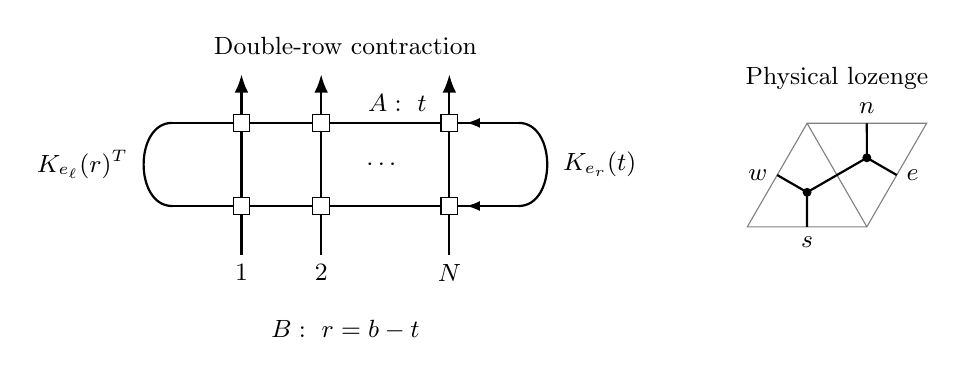
\begin{tikzpicture}[scale=.88,>=Latex,font=\small]
  \draw[thick] (0,.65) -- (5,.65);
  \draw[thick] (0,1.85) -- (5,1.85);
  \draw[->] (4.65,.65) -- (4.25,.65);
  \draw[->] (4.65,1.85) -- (4.25,1.85);
  \foreach \x/\lab in {1/1,2.15/2,4/N}{
    \draw[thick,->] (\x,-.05) -- (\x,2.55);
    \draw[fill=white] (\x-.12,.53) rectangle (\x+.12,.77);
    \draw[fill=white] (\x-.12,1.73) rectangle (\x+.12,1.97);
    \node[below] at (\x,-.05) {$\lab$};
  }
  \node at (3.05,1.25) {$\cdots$};
  \draw[thick] (0,.65) .. controls (-.55,.65) and (-.55,1.85) .. (0,1.85);
  \draw[thick] (5,.65) .. controls (5.55,.65) and (5.55,1.85) .. (5,1.85);
  \node[anchor=east,align=right] at (-.5,1.25) {$K_{e_\ell}(r)^T$};
  \node[anchor=west] at (5.5,1.25) {$K_{e_r}(t)$};
  \node[above] at (3.25,1.88) {$A:\ t$};
  \node[below] at (2.5,-.85) {$B:\ r=b-t$};
  \node[above] at (2.5,2.7) {Double-row contraction};
  \begin{scope}[shift={(8.3,.35)},scale=1.15]
    \coordinate (O) at (0,0);
    \coordinate (V) at (1.5,0);
    \coordinate (U) at (.75,1.299);
    \coordinate (UV) at (2.25,1.299);
    \coordinate (C1) at (.75,.433);
    \coordinate (C2) at (1.5,.866);
    \draw[gray] (O)--(V)--(UV)--(U)--cycle;
    \draw[gray] (U)--(V);
    \draw[thick] (.375,.6495)--(C1)--(.75,0);
    \draw[thick] (C1)--(C2);
    \draw[thick] (1.5,1.299)--(C2)--(1.875,.6495);
    \fill (C1) circle (1.6pt);
    \fill (C2) circle (1.6pt);
    \node[left] at (.375,.6495) {$w$};
    \node[below] at (.75,0) {$s$};
    \node[above] at (1.5,1.299) {$n$};
    \node[right] at (1.875,.6495) {$e$};
    \node[above] at (1.125,1.6) {Physical lozenge};
  \end{scope}
\end{tikzpicture}
\caption{The horizontal and vertical lines denote spin spaces, and the boundary curves denote the displayed tensors. The auxiliary row $B$ acts first on the site spins, then row $A$; products act from right to left. The two auxiliary ends are contracted with the displayed boundary tensors. This is a tensor schematic, whereas the inset shows the actual pair of equilateral triangles at the physical specialization. The black segments in the inset are the available honeycomb links, not one path configuration. The two dots are the centers counted by the path length: an $s$--$w$ or $e$--$n$ arc visits one center, and a single arc between the two pairs visits both.}
\label{fig:strip-double-row}
\end{figure}


We record local identities and their algebraic verification. Equalities are meromorphic (used first away from singularities). Let $P$ swap a pair of spin spaces, $F$ flip spins in a space, $J=\operatorname{diag}(-1,1,-1)$. Define
\[
 \begin{gathered}
 \Omega=\sum_p s^{-p}|p,-p\rangle,\qquad
 W|\pm\rangle=\kappa(|\pm,0\rangle+|0,\pm\rangle),\\
 W|0\rangle=|00\rangle+\kappa\sum_{p=\pm1}s^{-p}|p,-p\rangle,\quad Z=W^*=\bar W^T.
 \end{gathered}
\]
The image slots of $W$ will be indicated by a pair of labels (ordered); its input slot can then be regarded as a fused spin. We have
\begin{equation}
\begin{gathered}
 R_{21}(u)=R_{12}^T(u),\qquad R_{12}(u)R_{12}^T(-u)=I,\\
 R(u+\pi)=J_1 R(u)J_1,\qquad
 R(b-u)_{ij,kl}=s^{k-i}R(u)_{-i,l;-k,j},\\
 R(0)=P,\qquad R(b)=\Omega\bar\Omega^T,\qquad R(2L)=W Z.
\end{gathered}                                                   \label{eq:legacy-P-2}
\end{equation}
Indeed $Q(b-u)=Q(u)$, swapping $a,h$ and $c,d$ at reflected argument, which gives crossing by the displayed entries. Unitarity on the $\pm2,\pm1$ blocks uses $c(u)c(-u)=1$, $v(u)/a(u)=\sin u/S$ and $a(u)a(-u)=S^2/(S^2-\sin^2 u)$. On the zero block use additionally (prime denotes argument $-u$ here) $h+c h'=0$, $h h'+c d'+c' d=0$, by the sine products, and $s^2+s^{-2}=0$. Values in \eqref{eq:legacy-P-2} follow by substitution. Consequently
\[
 R_{23}(u-b)R_{13}(u)\Omega_{12}=\Omega_{12} I_3,
\]
where $I_3$ denotes the identity on slot 3 (by crossing, the output $(p,q,k)$ at input $j$ is $s^{-p}(R(u-b)R(b-u)^T)_{qk;-p,j}$).

The basic fusion identity and its adjoint are
\begin{equation}
 R_{23}(u-L)R_{13}(u+L)W_{12}=W_{12} R_{f3}(u),\qquad
 Z_{12} R_{13}(u+L)R_{23}(u-L)=R_{f3}(u) Z_{12},                \label{eq:legacy-P-3}
\end{equation}
where $f$ labels the fused space. Here and below adjoints can be taken at nonsingular real parameters first ($R$ Hermitian). We give details of the elementary check to fix normalizations. Multiply the first formula by $R_{32}(L-u)$ using \eqref{eq:legacy-P-2}, and write a subscript $+$ for argument $u+L$, primes for $L-u$, no decorations for $u$. Expanding on inputs $(f,3)$ gives the following sufficient equalities (spin-flipped inputs conjugate the same ones):
\[
\begin{array}{l|l}
 ++&cv'=c_+,\ cc'=v_+,\ ca'=a_+\\
 +0&v+a h'=v_+,\ vv'+aa'/\kappa=1,\ va'+av'/\kappa=a_+,\;\\
 &v h'+a d'=0,\ ac'=h_+\\
 0+&\kappa(a+v h')=a_+,\ av'+va'/\kappa=h_+,\ \kappa aa'+vv'=v_+,\;\\
 &a h'+v d'=c_+,\ vc'=d_+\\
 00&\kappa(a'+v'h)=h_+,\ v'+a'h=v_+,\ h'+\kappa h c'=\kappa a_+\\
 +-&h+\kappa c h'=\kappa h_+,\ hh'+\kappa(c d'+c'd)=0,\\
 &d v'+h a'=d_+,\;d a'+h v'=0,\text{ and the }++\text{ identities}.
\end{array}
\]
To verify, put $t_j=\sin(u+jL)$; the numerator rows and denominators are
\[
\begin{array}{c|rrrrr|l}
 &a&h&v&c&d&Q\\
 &-S t_{-3}&S t_0&-t_{-3}t_0&t_{-3}t_{-2}&t_0t_{-1}&t_2t_3\\
 '&S t_2&-S t_{-1}&-t_{-1}t_2&t_2t_1&t_{-1}t_0&-t_{-3}t_4\\
 +&-S t_{-2}&S t_1&-t_1t_{-2}&t_{-2}t_{-1}&t_1t_0&t_3t_4 .
\end{array}
\]
Thus $QQ'/Q_+=-t_{-3}t_2$. The $++$ row and $v h'+a d'=0$, $ac'=h_+$, $vc'=d_+$ follow immediately; for the other identities in rows $+0,0+$ use $t_{-2}t_2=t_0^2-S^2$, $t_{j-1}+t_{j+1}=t_j/\kappa$,
$t_{-3}t_4=t_0t_1-S^2/\kappa$, $t_3t_4=S^2/\kappa-t_0t_{-1}$, $t_0t_{-1}-t_{-2}t_1=\kappa S^2$. For the last two rows one also has
$t_2t_1-t_{-2}t_{-1}=t_0t_4/\kappa$,
$t_{-3}t_{-2}+t_2t_1=S^2/\kappa$, and can interchange primed and unprimed quantities (swaps $h_+,a_+$ and $d_+,c_+$).

These imply Yang--Baxter:
\[
 R_{12}(u-v) R_{13}(u) R_{23}(v)=R_{23}(v) R_{13}(u) R_{12}(u-v).
\]
Indeed at $u-v=0$ use the permutation; at $u-v=2L$ use $R(2L)=W Z$ and \eqref{eq:legacy-P-3}; at $u-v=b$ use \eqref{eq:legacy-P-2} and the analogous rank-one identity shown after \eqref{eq:legacy-P-2}, and its adjoint. At $u=0,2L$ reduce to the first two cases by multiplying on both sides by $R_{23}(v)^{-1}=R_{32}(-v)$ and permuting the labels (new order $1,3,2$). For generic fixed $v$ these give five values modulo $\pi$; clearing denominators, each entry has trigonometric degree $\le4$ in $u$ and is either periodic or antiperiodic by $\pi$ by \eqref{eq:legacy-P-2}, so vanishes identically.

\paragraph{Boundary fusion and reflection.}
The bulk identities are now available. The boundary identities needed to close and exchange rows (using a common variable $e$ for each equality) are, with $r=b-t$,
\[
 D_e(t)D_e(-t)=I,\qquad R(t-r) K_e(t)=P K_e(r),
\]
\begin{equation}
 \begin{split}
 D_{e,2}(t-L)R(2t)D_{e,1}(t+L)\bar W&=W D_e(t),\\
 W^T D_{e,2}(t+L)R(2t)D_{e,1}(t-L)&=D_e(t)\bar W^T .
 \end{split}                                                       \label{eq:legacy-P-4}
\end{equation}
In $D_{e,j}$ the second subscript just labels a slot. Unitarity of $D_e$ follows from $k(-t)=1/k(t)$, $l(-t)=-l(t)/k(t)$. To swap $K$, on total spin 0 and 1 the equalities reduce to $c(t-r) k(t)+h(t-r)=k(r)$ and $(v+a)(t-r)l(t)=l(r)$. Writing $y=t-\gamma$, these follow by
\[
 \sin(L-y)\sin(b-2y)+\sin(L+y)\sin(b+2y)=S\cos y,\qquad
 \cos(L\pm y)=\sin(b\mp y)
\]
on inserting the weights. For \eqref{eq:legacy-P-4}, the second identity follows from the first at real $t$ by conjugation, flipping all spins and swapping slots 1 and 2, then transposing ($J$ is not needed: $F\bar D_e F=D^T_{e/s}$ using formal real $e$). For the first, write subscripts $+,-$ on $k,l$ for $t\pm L$ and evaluate $a,h,v,c,d$ at $2t$. On expanding the three columns, the constant and linear terms in $e$ reduce respectively to
\[
 \begin{split}
 v k_+ +a=k,\qquad k_-(a k_+ +v)=k,\qquad k_-(h+\kappa c k_+)=\kappa;\\
 l_+ k_- c+k l_-=0,\qquad l_+(v+\kappa a)+\kappa l_- /k_-=\kappa l,\qquad
 l_+ k_-(a+\kappa v)+l_-=\kappa l,\\
 l_+ k_-(h+d)=l,\qquad \kappa\big((1+h)l_++k l_-/k_-\big)=l .
 \end{split}
\]
For example put $H_\pm=\sin(\gamma\pm t)$, $G_\pm=\cos(\gamma\pm t)$, $F_\pm=\sin(L/2\pm t)$, $P_\pm=\sin(2L\pm2t)$, $T_0=\sin(2t)$. Then $k_+=F_-/G_-$, $k_-=G_+/F_+$, $l_+=P_+/G_-$, $l_-=-P_-/F_+$; substitution gives the equalities by the sine products
\[
\begin{gathered}
 P_+ G_+-S G_-=T_0 F_-,\qquad P_+F_+-S F_-=T_0 G_-,\qquad
 2(H_+ F_+ P_+ -H_-F_-P_-)= S T_0/\kappa,\\
 P_- H_+-S H_-=T_0 F_-,\quad \kappa H_- -F_-=\kappa F_+,\quad H_-=\kappa(F_-+G_+),\quad
 S+\sin(2t-L)=2F_+G_-,\\
 P_+ H_+ G_+-P_- H_- G_-=\cos L\,T_0\cos(2t).
\end{gathered}
\]

We will use the reflection relation
\begin{equation}
 R(t-y) D_{e,1}(t) R(t+y)^T D_{e,2}(y)
 =D_{e,2}(y)R(t+y)D_{e,1}(t)R(t-y)^T.                            \label{eq:legacy-P-5}
\end{equation}
Here is a polynomial check using \eqref{eq:legacy-P-4}. Fix generic $y$. At $t=y,-y$ use $R(0)=P$ and $D_e(y)\allowbreak D_e(-y)=I$; at $t=0,4L$ use $D_e=I,J$ respectively, and \eqref{eq:legacy-P-2}. At $t-y=2L$ the right side is $W D_e((t+y)/2)W^T$ by \eqref{eq:legacy-P-4} and the left is the same (swap 1,2 in the second relation of \eqref{eq:legacy-P-4}, using $PW=\bar W$). This also gives \eqref{eq:legacy-P-5} at $t+y=2L$ using $y\mapsto-y$ and $D_e(y)D_e(-y)=I$. At $t-y=b$ the right side is $\Omega \Omega^T$, since
\[
 D_{e,2}(y) R(t+y)D_{e,1}(t)\bar\Omega
 =D_{e,2}(y)R(t+y)K_e(t)
 =P D_{e,1}(y)K_e(-y)=\Omega .
\]
This last equality also holds with both $D$'s transposed (flip both spins and conjugate, rescaling $e$), giving the same left side of \eqref{eq:legacy-P-5}. After clearing denominators the difference in \eqref{eq:legacy-P-5} has degree $\le 6$ in $t$, entries periodic or antiperiodic by $\pi$ (after clearing, $D_{e,1}$ transforms by conjugation by $J_1$ and a sign $-$); hence the seven checks suffice.

\subsection{Commuting and fusing double rows}\label{sec:strip-double-row-identities}
We now derive identities for $T$ by row exchange. Yang--Baxter gives
$R_{ij}(u-v) U_i(u)U_j(v)=U_j(v)U_i(u) R_{ij}(u-v)$. In particular swapping the two rows of $T$ gives $T(t)=T(r)$: the input swap uses $R(t-r)K_e(t)=P K_e(r)$ and the output swap its $r,t$ version via unitarity. Also $T(t+\pi)=T(t)$ since $K_e(t+\pi)=J_1 J_2 K_e(t)$.

For $T(t)T(y)$, take labels $A,B,C,D'$ of parameters $t,r,y,b-y$ respectively (below write $D'$ for a label). To interchange the row pairs, exchange $BC,AC,BD',AD'$ in that order, acting on the right boundary vector $V=K_e(t)_{AB}K_e(y)_{CD'}$ ($e=e_r$) by the corresponding $R$ product. Invariance of the vector reduces by \eqref{eq:legacy-P-2} to
\[
 R_{AC}(t-y)R_{BC}(b-t-y)V
 =R_{BD'}^T(t-y)R_{AD'}^T(b-t-y)V .
\]
This is \eqref{eq:legacy-P-5} by crossing. Indeed identify a vector $X$ with the matrix with entries $s^{-m-n}X_{i,-m,j,-n}$ in row $i,j$ and column $m,n$. Under this identification $R_{BC}(b-t-y)V$ is $D_{e,1}(t) R(t+y)^T D_{e,2}(y)$ and $R_{AD'}^T(b-t-y)V$ is $D_{e,2}(y) R(t+y) D_{e,1}(t)$. The remaining $R$'s act on the left and right respectively as in \eqref{eq:legacy-P-5}. On the left boundary (covector written as a transposed column), the inverse-transposed exchanges appear, exactly the analogous computation with $t,r$ exchanged and $y,b-y$ exchanged, $e=e_\ell$. Thus all $T$ commute. Further $T(0)=T(4L)=I$: at $0$ the input is $K_e(0)=\bar\Omega=P\Omega$ and the two rows act trivially on it by rank-one crossing after \eqref{eq:legacy-P-2}. The output pairing with this vector is 1. At $4L$, shift the second parameter $r$ by $\pi$ (conjugate that slot by $J$); the input becomes again $\bar\Omega$, the parameter difference again $b$ (higher parameter second), and the output pairing is 1.

For a product $T(t-L)T(t+L)$ use labels $B,C,A,D'$ with parameters $t-L,r+L,t+L,r-L$ in that order. Swap middle rows by $R_{CA}(r-t)$. We obtain product order $B A C D'$ between boundary column vectors $G_r,G_\ell$ (output transposed):
\[
 \begin{split}
 G_r &= R_{CA}(b-2t) K_{e_r}(t-L)_{BC} K_{e_r}(t+L)_{AD'},\\
 G_\ell &= R_{CA}(b-2r) K_{e_\ell}(r+L)_{BC} K_{e_\ell}(r-L)_{AD'} .
 \end{split}
\]
With fused slots $f,g'$ for $AB,C D'$ respectively, \eqref{eq:legacy-P-4} gives
\[
 (1\otimes Z_{C D'})G_r=(W_{AB}\otimes1)K_{e_r}(t)_{f g'},\qquad
 (W_{AB}^T\otimes1)G_\ell=(1\otimes Z_{C D'}^T)K_{e_\ell}(r)_{f g'} .
\]
Indeed the matrix given by $s^{-m-n} (G_r)_{p q;-m,-n}$ (slots indexed $AB;C D'$, columns ordered $n,m$) by crossing is $D_{e_r,2}(t-L) R(2t) D_{e_r,1}(t+L)$, and similarly for $G_\ell$ with $r,+L,-L$. Also $Z_{-j;-m,-n}=\bar W_{n,m;j}$ and it is zero unless $j=m+n$.

By \eqref{eq:legacy-P-3}, $U_B U_A$ preserves the $W_{AB}$ subspace acting by $U_f(t)$, and $U_C U_{D'}$ preserves $\ker Z_{C D'}$ acting on the quotient by $U_{g'}(r)$. Moreover:

\begin{itemize}

\item 

At $t=L-\xi_i$ the local product $R_{Bi}(0) R_{Ai}(2L)$ has range in $W_{AB}$, hence so does $U_B U_A$.

\item 

At $t=L+\xi_i$ the local product $R_{Ci}(b) R_{D'i}(L)$ kills $\ker Z_{C D'}$, hence so does $U_C U_{D'}$. Indeed its adjoint has range in the image of $W_{C D'}$: $R_{D'i}(L)$ maps $\Omega_{Ci}$ into this image by crossing at $u=2L$, $R(2L)=WZ$ (output $c,d,j$ for input $v$ on $D'$ has coefficient $s^{-c}R(L)_{dj;v,-c}=s^j R(2L)_{cd;-j,v}$).

\end{itemize}

Consequently at either of those values the contracted product reduces to $T(t)$. Indeed the part of $G_r$ in arbitrary slots $AB$ tensor $\ker Z_{CD'}$ is then harmless (either killed, or mapped to $W_{AB}\otimes\ker Z_{CD'}$ annihilated by the output); the rest can be lifted through $W_{AB}$ from $K_{e_r}(t)_{f g'}$, and \eqref{eq:legacy-P-3} and the formula for $G_\ell$ give precisely $T(t)$. We have shown, first for generic rapidities,
\begin{equation}
 T(t-L)T(t+L)=T(t)\quad\text{at }t=L\pm\xi_i.                     \label{eq:legacy-P-6}
\end{equation}

\subsection{The scalar crossing function}\label{sec:strip-scalar}

The row identities now have to be connected to the positive path sum. The next statement collects the scalar data that will enter the finite functional.

\begin{auxlemma}[Scalar crossing function]
At the homogeneous rapidities $\xi_1=\cdots=\xi_N=-L/2$, the double-row family determines an even, $\pi$-periodic meromorphic function $p$ with $p(0)=2B_N$. It is rational in $X=\cos(2u)$, with polynomial part $4X+\rho$ for a constant $\rho$, and denominator dividing
\[
 (X+1)^N(X+\cos 2L)^{N+1}.
\]
Moreover $p(3L/2)=p(5L/2)=0$, and
\[
 p(u-L)+p(u+L)-p(u)
\]
has a zero of order at least $2N$ at $u=0$ and of order at least $N$ at $u=L$.
\end{auxlemma}
\begin{proof}
We construct the scalar function through the physical path expansion and then verify its rational form and zero multiplicities.

\paragraph{Loop cancellation.}
The finite matrix identities alone do not identify a walk partition function. To extract the relevant eigenvalue of the commuting family, specialize first to $e_\ell=e_r=0$. Matrix products have a planar oriented-path expansion on the square tensor diagram of Figure~\ref{fig:strip-double-row}. Positive horizontal arrows are right-to-left and positive vertical arrows upward. In a tile, allowed arc configurations, with orientation ignored, are empty (weight 1), a single e-n or s-w ($a$), a single e-s or n-w ($h$), a single straight across ($v$), or both e-n, s-w ($c$) or both e-s, n-w ($d$). The entries of $R$ give these weights times phases, summed over choices: all arc phases are 1 except for e-to-s, whose phase is $s$, and n-to-w, whose phase is $s^{-1}$ (reverse arrows conjugate the phases). At the left and right boundaries $K_0$ permits empty or a U-turn between the double row's two terminals, the latter with weight $k$ and phase $s$ if the upper arrow is positive ($s^{-1}$ otherwise). These phase assignments have product $s^{\pm2}$ on any simple closed path, and product 1 on a simple bridge from a right endpoint to a left endpoint in a rectangle, with only the hard walls (no U-turns). For instance give each arc phase $\exp(i\,\Delta/4)$ where $\Delta$ is its rotation of tangent (starting and ending orthogonally to tile edges), plus $\pi/2$ at terminal vertical arrows, minus $\pi/2$ at initial vertical arrows. These corrections telescope; take quarter circles and straight lines and smooth boundary turns as needed. Bridges have total turn 0 by simplicity (close using the boundary). Thus, summing orientations, closed loops cancel. This holds for arbitrary spectral parameters at zero boundary variables. In particular every product of double rows at those variables has empty-site-to-empty-site entry 1.

At $t=\gamma$ and $\xi_i=-L/2$, the boundary weights $k$ are zero, and the tile weights are evaluated at $L$, giving $a=\kappa$, $h=v=c=\kappa^2$, $d=0$. These are precisely hard-wall honeycomb paths through triangular pairs: s-w and e-n each visit the center of one triangle, distinct when both are used; each of the other single arcs visits both centers. The square drawing is topological; the inset of Figure~\ref{fig:strip-double-row} shows the actual honeycomb geometry.

\paragraph{A signed flux bound.}\label{sec:strip-flux}
We next obtain positive path bounds at these weights. The calculation is the local parafermionic cancellation of \cite[Lemma~1]{DuminilCopinSmirnov2012}, written in our signed exit-flux convention. It uses the physical honeycomb turning angle, rather than the oriented-loop phases above. In any finite lozenge rectangle and with one starting boundary midpoint, the sum of weights of paths to the rest of the boundary is at most $1/\cos(3\pi/8)$. Indeed insert in each such path weight (including in prefixes) the factor $\exp(i\beta W_{\rm turn})$, $\beta=3/8$, $W_{\rm turn}$ total turn in actual honeycomb geometry. At each triangle center, the total signed flux of prefixes into it (ending at an incident midpoint heading toward it, including the initial flux 1 at the source) equals the flux out of it. If unvisited the two continuations sum back to the entering weight by $2\kappa\cos L=1$. The incoming terms where the vertex has been visited cancel in pairs: there is a stem into the vertex followed by the unfinished simple loop back to its third half-edge; reversing the loop, the changes of turn from the stem are $+4\pi/3$ and $-4\pi/3$. Indeed the stem arrives from outside the loop by simplicity and the boundary start; for a completed positively oriented loop the turn at this vertex would be $+\pi/3$, but departure there from the stem instead gives $-\pi/3$. (Weights in the pair have thus opposite phases.) This proves the flux rule, hence total signed exit mass 1. Turns to the boundary are in $[-\pi,\pi]$ by convexity and simplicity (close from the end to the start along the perimeter; besides the arc turn there are two turns by $\pi/2$ with common sign and the boundary direction change). This gives the bound by real parts.

\paragraph{Decay at fixed width.}
With width fixed, path weight from a fixed bottom midpoint to the opposite top boundary of taller and taller lozenge rectangles tends to 0. Indeed to each top exit append in an extra row a deterministic continuation to a lateral wall (one turn s-w and then e-w straight crossings as necessary), staying there in new triangles, at cost bounded below depending only on width. This is injective for each height and sends different heights to different endpoints. Total exit mass to the lateral boundaries in the semi-infinite rectangle is bounded by the preceding flux argument and exhaustion. All bottom arch weights in the semi-infinite rectangle (analogously top arch weights) are summable by the same bound.

\paragraph{The common eigenline.}
Now every entry of $T(\gamma)^m$ in this specialization is an oriented sum of path systems between the specified occupied top/bottom midpoints of the rectangle of height $2m$ (no detached loops). Systems containing at least one bottom-to-top path contribute vanishingly as $m\to\infty$, by bounding by products of the preceding single-path sums; the pure bottom and top arches converge to independent half-strip systems by the summability (phases included). Consequently $T(\gamma)^m$ tends to a rank-one projection with empty-empty entry 1. Writing $\mathbf0$ for the empty site-spin state, we have
\[
 T(\gamma)^m\longrightarrow P_0,\qquad \rank P_0=1,\qquad (P_0)_{\mathbf0,\mathbf0}=1.
\]
Thus $1$ is a simple eigenvalue and the rest of the spectrum lies strictly inside the unit circle.

For rapidities near this specialization we can analytically continue that simple eigenline of $T(\gamma)$ (and its eigenprojection), also over the square-zero boundary variables by expansion. At zero boundary variables the simple eigenvalue is still 1: all empty-empty entries of powers remain 1 by loop cancellation, while the other spectral part decays. The corresponding projection thus has empty-empty entry 1. 

Since all $T(t)$ commute (modulo $e_\ell^2=e_r^2=0$), this is a common eigenline, and at zero variables the eigenvalue of every $T(t)$ on it is 1 as well (take the empty-empty entries of $T(t)T(\gamma)^m$). 

The linear terms of the common-line eigenvalue vanish because at zero variables the right and dual lines of the projection are in the spin-zero site sector (by total-spin conservation and the nonzero empty-empty entry); linear terms of $T(t)$ change the site's total spin by 1 up or down. Thus the eigenvalue is of the form $1+e_\ell e_r q(t;\xi)$; here $q$ can be computed by contraction of $T(t)$ with vectors independent of $t$ (or trace against the rank-one projection including nilpotents, for instance defined by the Taylor expansion at zero boundary variables of an ordinary simple-pole resolvent projection). At the homogeneous rapidities, the spectral decomposition gives
\[
 [e_\ell e_r]\,(T(\gamma)^m)_{\mathbf0,\mathbf0}
 =m q(\gamma;\xi)+O(1).
\]
Indeed $(1+e_\ell e_rq)^m=1+m e_\ell e_rq$. The mixed coefficient of the continued eigenprojection contributes a term independent of $m$, and derivatives of the remaining spectral part decay by the gap.

There is also a direct path interpretation of this coefficient. Since $l(\gamma)=1$, it sums paths with one positive-arrow terminal on each wall of the $2m$-row rectangle, directed right-to-left and with phase one. Translation averaging and exhaustion therefore give
\[
 B_N=\lim_{m\to\infty}\frac{1}{2m}
 [e_\ell e_r]\,(T(\gamma)^m)_{\mathbf0,\mathbf0}
 =\frac12 q(\gamma;\xi).
\]
The factor two counts the rows in one transfer step.

\paragraph{Rational dependence on the spectral parameter.}
We have identified $q(\gamma)=2B_N$ at the homogeneous physical specialization. Its spectral-parameter dependence now supplies the interpolation conditions. For fixed $\xi$, $q(t;\xi)$ is invariant by $t\mapsto b-t,t+\pi$, by the identities for $T$. From $T$ its denominator thus divides, with $u=t-\gamma$ and $X=\cos(2u)$,
\[
 (X+\cos 2L)\prod_i (X+\cos(2\xi_i+L))(X+\cos(2\xi_i-L)).
\]
Indeed these factors are the paired sine denominators of $K,R$ at reflected arguments, giving polynomials in $X$ after clearing them. As $t=\gamma+iY$, $Y\to\infty$, the coefficient of growth in $q$ comes only from the $e_\ell e_r$ part of $T(t)$ since the $R$'s and $k$'s stay bounded and $l(t),l(b-t)\sim\exp(Y)$. Divided by $l(t)l(b-t)$ this part tends on total site spin 0 to twice identity. In fact the first row's $R$ has $v\to1$, $a,h\to0$, $d\to c^{-1}$ in the sense of reciprocal limiting phases, and has only the possible limiting off-diagonal transition of auxiliary spin $+1$ to $-1$ ($c+d/s^2\to0$); the other row is reversed. The auxiliary spin pairs in this coefficient must both be $+0$ or $0+$, so only diagonal elements survive and their products are 1 on the indicated sector. Hence $q\sim 4 X$.

Putting $p(u)=q(\gamma+u;\xi)$ now at homogeneous $\xi$, we have obtained a rational function of $X$ with polynomial part $4X+\rho$ and denominator dividing $(X+1)^N(X+\cos 2L)^{N+1}$. From $T(0),T(4L)$ we have $p(3L/2)=p(5L/2)=0$. From \eqref{eq:legacy-P-6}, before taking the homogeneous limit, the even function
\[
 q(\gamma+u-L;\xi)+q(\gamma+u+L;\xi)-q(\gamma+u;\xi)
\]
vanishes at $u=L/2\pm\xi_i$. It is analytic near $u=0,L$ for $\xi$ near the homogeneous point. Thus in the homogeneous limit $p(u-L)+p(u+L)-p(u)$ has a zero of multiplicity at least $2N$ at 0 and at least $N$ at $L$ (use generic distinct nodes first, including the even reflections of the ones near 0).

\end{proof}

\subsection{The finite functional}

\begin{proof}[Proof of Theorem~\ref{thm:strip-functional}]
The scalar function constructed in Section~\ref{sec:strip-scalar} can now be represented by the asserted functional. Partial fractions give, on $|\operatorname{Re}u|\le5L/2$, $p(u)=\mathcal L(C_u/D)$ for some $f\in M+\mathbf C g$ and $\rho$ as in \eqref{eq:legacy-P-1}. Indeed
\[
 \int_0^\infty\frac{\cosh(uz)\sinh(mz)}{\sinh(\pi z/2)}\,dz
 =\frac{\tan(m+u)+\tan(m-u)}2=\frac{\sin 2m}{X+\cos 2m},
\]
near $m=0,L$. The integral follows e.g. by geometric expansion of the denominator and the partial fractions for $\tan y$ (from the ordinary sine product or a rectangular residue contour); convergence is absolute. Derivatives $1,3,\ldots,2N-1$ at $m=0$ and $0,1,\ldots,N$ at $L$ span precisely the required polar parts. After division by the factor $z$ in the measure, the first family gives $1,x,\ldots,x^{N-1}$. In the second family, derivative order zero gives $g$, and orders $1,\ldots,N$ give the derivatives of $C_m$ at $m=L$ spanning the other half of $M$. The atoms at $-4$ and $0$ supply $4X$ and $\rho$, respectively.

Then
\[
 p(u-L)+p(u+L)-p(u)=\mathcal L(C_u),
\]
so the multiplicities give $\mathcal L(M)=0$, and $p(3L/2),p(5L/2)=0$ give the other vanishing conditions since $C_{3L/2}/D=C_{L/2}$ and $C_{5L/2}/D=C_{3L/2}+C_{L/2}-C_{L/2}/D$. This completes \eqref{eq:legacy-P-1}.

\end{proof}

\section{Positive interpolation and the strip exponent}\label{c6:strip-asymptotics}

Positive interpolation turns the finite strip functional into averages under a determinant density. We estimate its characteristic products and interpolation residuals to obtain $B_N\asymp N^{-1/4}$. 

\subsection{A positive determinant formula}
Retain the measure and spaces in \eqref{eq:legacy-P-1}, and put
\[
 \begin{gathered}
 c_1=C_{L/2},\quad c_3=C_{3L/2},\quad h_0=1/D,\quad h_1=c_1/D,\\
 F_0=M+\mathbf R c_1,\quad F=F_0+\mathbf R c_3,\quad G=M+\mathbf R g
 \end{gathered}
\]
(using real spans in the following). Here $N$ remains the strip width, while $d=\dim F_0=2N+1$ is the number of interpolation nodes. A complete jet at a label of multiplicity $k$ consists of derivatives of orders $0,\ldots,k-1$. Use jets of $C_{\sqrt\beta}(x)$ in $\beta$ as bases, ordered first by $\beta$, then by derivative order. Thus $M$ takes labels $0,L^2$ each with multiplicity $N$; the $g$ basis row in $G$ is inserted between. For $X=(x_1<\dots<x_d)$ in $(0,\infty)$, let $\nu$ denote the probability proportional to
\[
 \det F_0(X)\det G(X)\prod_i d\mu(x_i)
\]
(evaluation matrix with functions as rows). Indeed $g=\int_0^L C_t\,dt$, so the $G$ determinant integrates that for $G_t=M+\mathbf R C_t$, $0<t<L$. \begin{lemma}[Positive jet interpolation]\label{lemma:jet-interpolation}
All ordered jet determinants formed from complete jets of $C_{\sqrt\beta}(x)$ at nonnegative ordered labels are positive at distinct positive ordered points and remain nonnegative at confluent nonnegative points. Complete jet spaces are Chebyshev spaces on $[0,\infty)$, counting multiplicities.\end{lemma}
\begin{proof}
All ordered jet determinants are positive at ordered nonnegative points (also confluently, with derivatives at repeated points). This follows from the nonnegative Taylor minor expansion using $C_{\sqrt\beta}(x)=\sum_j \beta^j x^j/(2j)!$, with strictly positive first consecutive-degree term. Here generalized power determinants of increasing nonnegative integer powers at positive ordered points are strictly positive: a combination of $n$ powers has at most $n-1$ zeros counting multiplicity (divide by the first and differentiate successively/Rolle), and the sign is positive e.g. by coalescing near 1 (Wronskian). Confluent cases at zero are nonnegative by limits. In particular the spaces of complete jets are Chebyshev counting multiplicities on $[0,\infty)$. All Gram entries pairing a row from $F$ or $h_0,h_1$ and one from $G$ are finite (the density in $p=\sqrt{x}$ decays at rate $b=3L$).
\end{proof}

Write $e_y H=H(y)-I_{F_0,X}H(y)$ for evaluation minus interpolation at $X$ using $F_0$. Also use $E_y H=H(y)-I_{F,(0,X)}H(y)$. The determinant integrations below are instances of Andr\'eief's identity; see \cite[Equation~(1.3)]{TracyWidom1998}. We retain the interpolation calculation to fix its oblique projection and evaluation columns. Gram/Cramer identities using \eqref{eq:legacy-P-1} give, for $s_*=\rho/(4a_*)$ there,
\[
 \mathcal L(H)/(4a_*)=\nu[e_{-4}H]+s_*\nu[e_0 H].
\]
Indeed integrating a determinant product gives the determinant of the pairings by multilinearity, so the mean interpolant is the unique linear projection onto $F_0$ preserving the moments against $G$. Also
\[
 \nu[e_0 c_3]\,\nu[e_{-4}h_0]-\nu[e_{-4}c_3]\,\nu[e_0 h_0]
 =\nu[(e_0 c_3) E_{-4}h_0].
\]
For this append rows $c_3,h_0$ and evaluation columns $0,-4$ to the $F_0$ determinant and integrate against $\det G(X)$ (Schur complement). Since $d$ is odd, $e_0 c_3<0$ by ordered jet positivity. Let $\nu_3$ be the tilt of $\nu$ by $-e_0 c_3$. It will suffice to show
\begin{equation}
 \begin{gathered}
 \nu[-e_0 c_3]\gtrsim N^{-1/2},\qquad |\nu[e_0 h_i]|\le N^{-1+o(1)},\qquad
 |\nu[e_{-4}h_i]|=O(1)\quad (i=0,1),\\
 \nu_3[E_{-4} h_0]\asymp N^{-1/4}.
 \end{gathered}                                                     \label{eq:legacy-P-7}
\end{equation}
For the elimination, abbreviate
\[
 A_y=\nu[e_yc_3],\qquad H_{j,y}=\nu[e_yh_j]
 \quad(y=0,-4;\ j=0,1).
\]
The condition $\mathcal L(c_3-h_1)=0$ gives
\[
 s_*=-\frac{A_{-4}-H_{1,-4}}{A_0-H_{1,0}},
\]
whenever the denominator is nonzero. The determinant identity above, together with the definition of $\nu_3$, then gives the exact formula
\[
 \frac{\mathcal L(h_0)}{4a_*}
 =\frac{A_0\nu_3[E_{-4}h_0]
        +H_{1,-4}H_{0,0}-H_{1,0}H_{0,-4}}
       {A_0-H_{1,0}}.
\]
The estimates in \eqref{eq:legacy-P-7} imply that $|A_0|\gtrsim N^{-1/2}$ and $|H_{1,0}|\le N^{-1+o(1)}$. Hence the denominator is nonzero for large $N$, the coefficient of the positive residual is $1+O(N^{-1/2+o(1)})$, and the remaining quotient is $O(N^{-1/2+o(1)})$. The estimate for $\nu_3[E_{-4}h_0]$ therefore proves $B_N\asymp N^{-1/4}$.

\subsection{Characteristic products}

\begin{lemma}[Characteristic products]\label{lemma:characteristic-products}
The following characteristic-product estimates hold for both $\eta=\nu,\nu_3$. Put $r(x)=(x+y^2)/(x+z^2)$. We claim
\begin{equation}
 \eta\left[\prod_i r(x_i)\right]\asymp N^{b(y-z)/\pi}\qquad (0<y<z\text{ fixed}).                 \label{eq:legacy-P-8}
\end{equation}
In the separate growing-parameter regime $y^2=2z^2=2N^{3/2}$, where $1\le r\le2$, the expectation is at most $\exp(o(N))$. \end{lemma}

We isolate the elementary identity used in its proof, so that the polynomial comparison has an explicit starting point.
\begin{lemma}[Polynomial generating identity]\label{lemma:polynomial-generating}
Let $c>0$ and let $\mu_c$ be the probability measure proportional to $dp/\cosh(cp)$ on $p=\sqrt{x}>0$, and put $\alpha=\pi/(2c)$. Then
\begin{equation}
 A_m(x)=\cos(\alpha m)C_m(x),\quad w_m=\tan^2(\alpha m),\quad
 \int A_mA_n\,d\mu_c=1/(1-w_mw_n)
 \label{eq:legacy-P-9}
\end{equation}
for real $|m|+|n|<c$.
\end{lemma}
\begin{proof}
The elementary transform of $1/\cosh(cp)$ follows by integrating on the full line and shifting by $i\pi/c$, picking the simple pole. It gives
\[
 \int C_m C_n\,d\mu_c
 =\tfrac12\bigl(\sec(\alpha(m+n))+\sec(\alpha(m-n))\bigr).
\]
Multiplying by $\cos(\alpha m)\cos(\alpha n)$ and combining the two fractions gives the identity.
\end{proof}

\begin{proof}[Proof of Lemma~\ref{lemma:characteristic-products}]
We reduce the two determinant densities to symmetric pairs before evaluating their characteristic products.
\paragraph{Reduction by interlacing.}
It suffices to estimate with $g$ replaced by any $C_t$, $0<t<L$, uniformly in $t$. The row and column spaces for the point density are then respectively $(F_0,G_t)$ or $(A,G_t)$, where $A=\{f\in F:f(0)=0\}$ (the $-e_0 c_3$ factor extends the first determinant at column 0). They contain symmetric subspace pairs $(M,M)$ or $(U,U)$ respectively, $U=\{f\in M:f(0)=0\}$.

Here are details justifying comparison to the determinant-product densities of those symmetric pairs. For spaces $V,B$ of common dimension as above, consider the roots of
\[
 \det \int V B^T(x-\lambda)d\mu'(x),\qquad d\mu'=d\mu/(x+z^2)
\]
(function bases as column vectors in the Gram formula). The expectation in \eqref{eq:legacy-P-8} is $\prod_j r(\lambda_j)$. The roots for $(F_0,G_t)$ interlace those for $(M,M)$; similarly we can successively interlace along the chain
\[
 (U,U)\ \,\subset\ \, (F_0\cap\{f(0)=0\},M)\ \,\subset\ \, (A,G_t).
\]

To see this, each space along the chains is Chebyshev on the positive interval counting multiplicities, with a nested Chebyshev flag of all lower dimensions there (truncate jets, retaining constant first, then impose the zero at 0 when present). Gram determinants are nonzero by determinant integration. A nonzero real analytic function orthogonal to such a dimension-$m$ space must have at least $m$ sign changes: otherwise use the flag to put simple zeros of a test function just at its changes of sign, with no other zeros. Thus a real root $\lambda$ is positive: for such a root there is a nonzero real $a\in V$ with $(x-\lambda)a\perp B$, whereas $a$ by itself has at most $m-1$ flips ($m=\dim V=\dim B$). Non-real roots cannot occur either. Otherwise for some nonzero complexified $a\in V$, $(x-\lambda)a$ is orthogonal to $B$. For almost every phase $\theta$, its rotated real part needs at least $m$ sign changes. But averaging on any finite grid of positive points off zeros of $a$, the mean number of flips of $\operatorname{Re}(e^{i\theta}(x-\lambda)a)$ is bounded by the mean for $\operatorname{Re}(e^{i\theta}a)$ plus $\pi^{-1}$ times the variation of $\arg(x-\lambda)$ on the whole positive ray (a pair contributes its circular angle distance divided by $\pi$). This is bounded by $m-1$ plus a number strictly less than 1. Exhausting a dense grid gives a contradiction. Moreover consecutive pairs of nested spaces in the chains cannot share a positive root: take a real root function $a$ of the smaller first space and a real dual root function $h$ of the larger second space. By the same sign-change argument $h$ cannot belong to the smaller second space. But $(x-\lambda)a$ is orthogonal also to $h$, thus to the full larger second space, again impossible by signs.

Now continuously contract all positive jet labels to zero by common scaling. The spans limit to the ordinary consecutive polynomial spaces starting with 1 (or with $x$, when the vanishing at 0 was imposed). This convergence, also for Gram pairings, follows by taking Newton divided differences in $\beta$ (including at multiplicities), with exponential domination, subtracting constants where we impose vanishing. All roots are continuous as unordered multisets to that limit. At the polynomial limit interlacing is strict: the matrices give the usual positive-weight orthogonal polynomial roots for degrees equal to space dimensions, with weights $\mu'$ for the first chain and $x^2\mu',x\mu',x\mu'$ along the second. Consecutive degrees for a common weight interlace (symmetric multiplication compressions and no common roots by the sign argument); between the first and second weights of the latter chain use that the degree-$k-1$ polynomial for $x^2\mu'$ is proportional to $(p_k-\frac{p_k(0)}{p_{k-1}(0)}p_{k-1})/x$ for the $x\mu'$ polynomials $p_j$, so interlaces $p_k$. Here the compression characteristic polynomial is the orthogonal polynomial, e.g. by the sign/orthogonality relation $(x-\lambda)a\perp$ lower degrees. Throughout the deformation all roots remain real, and roots at adjacent levels cannot coincide. A root therefore cannot pass one from an adjacent level, so this interlacing persists. Since $\log r$ is monotone with bounded range in each application, products along adjacent interlacing levels differ by bounded factors, also in the growing-$z$ case. This proves the desired reduction to the symmetric pairs, uniformly.

\paragraph{Comparison with polynomial spaces.}
For the symmetric spaces $H=M$ or $U$, we now compare with ordinary polynomials in the original measure $\mu$. The product expectation is the determinant of the compression of the positive multiplication $r$ to $H$ in $L^2(\mu)$. It can be bracketed (up to constant factors) by polynomial compression determinants of orders $N$ and $CN$ for a sufficiently large fixed $C$. Indeed, if $\mathcal P_{<n}$ denotes polynomials of degree $<n$, then
\[
 \mathcal P_{<N}\cap\{f:f(0)=0\}\subset H,
\]
so the lower-dimensional comparison loses only one polynomial direction. For the comparison with the larger polynomial space, $M$ is approximable in the polynomials of degree $<CN$ with operator-norm error $\le e^{-N}$ in $L^2(\mu)$, as proved just below. Such approximation identifies $H$ almost isometrically with a subspace there, changing the determinant by a $1+o(1)$ factor since $r,r^{-1}$ are bounded uniformly. Determinants decrease under enlarging a space if $0<r\le1$, and increase if $r\ge1$, with codimension-one change bounded (e.g. by Schur complements).

For the approximation and polynomial estimates use the probability measures $\mu_c$ and the generating identity of Lemma~\ref{lemma:polynomial-generating}. Thus $A_m=\sum_{j\ge0} P_j(x)w_m^j$ near zero gives orthonormal polynomials $P_j$ of degree $j$. For $|m|<c/2$ this is the $L^2$ expansion also with derivatives (compare coefficients and norms by \eqref{eq:legacy-P-9}). Take $2L<c<b$. Elements $h\in M$ then have coefficients supported on $j<N$ plus sequences $q^j p_0(j)$ with $q=w_L<1$, polynomial $p_0$ of degree $<N$. For $\|h\|_{\mu_c}=1$, $|p_0(j)|\le q^{-j}$ at $j=N,\ldots,2N-1$. Lagrange interpolation bounds $|p_0(j)|\le q^{-2N}(C_1 j/N)^N$ at higher $j$, so beyond $D_0=C_2N$ the coefficients decay as $e^{-c_1 j}$. Polynomials $P_j(p^2)$ themselves are bounded by $C_3^{j+1} e^{cp/4}$ by taking a sufficiently small circle in the generating formula for $w_m$. Hence the polynomial projection through order $D_0$ has negligible $\mu_c$-norm tail at $p>C_4N$ for $C_4$ large; $h$ itself has a positive fraction of norm on $p\le C_4N$. There $\mu\gtrsim e^{-C_5 N}\mu_c$, while globally $\mu\lesssim\mu_c$. Projecting through degree $CN$ now with still larger $C$ gives the asserted exponentially good relative error in $L^2(\mu)$.

\paragraph{Evaluating the polynomial determinants.}
It remains to evaluate polynomial compression determinants. For polynomial space of degree $<n$, denote the product ratio/expectation by $R_{W,n}(r)$ for base weight $W$. One has
\[
 R_{W,n}(r^2)=K_{n,W'}(-y^2)/K_{n,W'}(-z^2),\quad
 K_{n,W'}(x)=\sup_{\deg h\le n}\frac{|h(x)|^2}{\int |h|^2dW'},\quad dW'=dW/(x+z^2)^2
\]
(using weights as measures). This is the Gram cofactor identity on degrees $\le n$ for the hyperplanes spanned by $(x+y^2)x^j$ and $(x+z^2)x^j$, $0\le j<n$, whose coefficient minors are evaluation vectors up to sign. For $c=b$ we have $K_{n,\mu_c}(-y^2)\asymp n^{2c y/\pi}$ when $y>0$ is fixed. Indeed sum $|P_j(-y^2)|^2$ via their even generating series in $u$ with $w_m=-u^2$,
\[
 (1-u^2)^{-1/2}\cosh(2s\operatorname{arctanh}u),\qquad s=cy/\pi.
\]
On the unit disk near $u=\pm1$ its absolute value is comparable to $|1\mp u|^{-s-1/2}$, elsewhere near the circle bounded. Thus the squared-coefficient sum with radial weights $r_0^{4j}$ grows as $(1-r_0)^{-2s}$ by circle integration. For truncation take $r_0=\exp(-1/n)$ (upper), then $r_0=\exp(-A/n)$ for a large fixed $A$ (lower, tail beyond $n$ bounded by $C n^{2s}\sum_{k\ge0}2^{2ks} e^{-4\cdot2^k A}\ll (n/A)^{2s}$ by the upper estimate).

For fixed positive $y,z$ and $W=\mu$ or $r\mu$, $W'$ is bounded between constants times $\mu_b/(x+Y^2)^2$ and $\mu_b$, for a fixed $Y>\max(y,z)$. We still have $K_{n,W'}(-v^2)\asymp n^{2s_v}$ for $v=y,z$, where $s_v=bv/\pi$. For the needed upper bound divide the polynomials of degree $\le n$ by $x+Y^2$ and use the $\mu_b$ norm on the resulting span (degrees $<n$ plus $g_Y=1/(x+Y^2)$). The coefficients $b_j$ of $g_Y$ on the orthonormal $P_j$ above ($c=b$) are
\[
 b_j=\frac1Y\int_0^\infty e^{-Ym}\frac{(-\tanh^2(\alpha m))^j}{\cosh(\alpha m)}dm,\qquad
 |b_j|\asymp (j+1)^{-1/2-s_Y}.
\]
Indeed $g_Y(x)=Y^{-1}\int_0^\infty e^{-Ym}\cos(m\sqrt x)dm$, and \eqref{eq:legacy-P-9} extends to imaginary $m$ paired against parameters near zero. The bounds follow substituting $v'=e^{-2\alpha m}$ (integral comparable to that of $v'^{s_Y-1/2}((1-v')/(1+v'))^{2j}$ over $(0,1)$, split near $v'\asymp1/(j+1)$ or use exponential decay above this scale). At $-v^2$, dyadic Cauchy--Schwarz and the polynomial kernel bound give $\sum_{j\ge n}|b_j P_j(-v^2)|=O(n^{s_v-s_Y})$. The full sum evaluates to $g_Y(-v^2)$ by inserting the integral, using this absolute bound (integral signs fixed for each coefficient) and the generating series at $u=\tanh(\alpha m)$. Thus after orthogonal projection onto degrees $<n$ the residual of $g_Y$ has evaluation $O(n^{s_v-s_Y})$ and its norm is at least $(\sum_{j\ge n}|b_j|^2)^{1/2}\gtrsim n^{-s_Y}$. This bounds the extra direction as required.

Consequently for $n=N$ or of order $CN$, $R_{W,n}(r^2)\asymp N^{2b(y-z)/\pi}$. Cauchy--Schwarz gives the upper bound for $R_{\mu,n}(r)$ with half exponent, and the matching lower since $R_{\mu,n}(r^2)=R_{\mu,n}(r)R_{r\mu,n}(r)$. When $y^2=2z^2=2N^{3/2}$, $W=\mu$, $W'\gtrsim z^{-4}\mu_{b+\varepsilon}$ for fixed $\varepsilon>0$, and $K_{n,W'}(-z^2)\gtrsim z^4$ by testing with a constant. The analogous generating series ($c=b+\varepsilon$) on $|u|=\exp(-1/n)$ gives $K_{n,\mu_{b+\varepsilon}}(-y^2)\le\exp(O((y+1)\log n))$, so $R_{\mu,n}(r)\le\exp(o(N))$. This proves all the product claims.
\end{proof}

In particular under either $\eta$ the probability of having $x_{N-1}<N^{3/2}$ is exponentially small (the growing-parameter product there is $\ge (3/2)^{N-1}$).

\subsection{Interpolation residuals}

The characteristic products will control the errors at $0$ and $-4$ once the following pointwise comparison is established.

\begin{auxlemma}[Residual product bounds] Take $e_{-a}$ for $a=0,4$, or $E_{-a}$ for $a=4$, and denote the relevant node set ($X$ or $\{0,X\}$) in increasing order by $v_i$. Write $\lambda_*=\pi/(3L)=8/3$. For large $N$ the residual is nonnegative on either $h_j$ and bounded above by
\begin{equation}
 C\prod_{i\text{ among first }N}\frac{v_i+a}{v_i+\lambda_*^2}.
                                                                    \label{eq:legacy-P-10}
\end{equation}
On $h_0$ there is also the lower bound with positive constant times the analogous product over all nodes. The constants are uniform in the ordered interpolation nodes.
\end{auxlemma}
\begin{proof}
First we reduce jet interpolation to monomial interpolation. To do so, translate to $w=x+a$ with evaluation at 0 (all interpolation nodes strictly positive after translation). In this coordinate each residual against the jet space is a convex combination of interpolation errors against monomial systems whose powers include $0,1,\ldots,N-1$, of the same size. Indeed take those powers first as basis polynomials; then in the Taylor expansion of the other basis functions the minors needed for Cauchy--Binet correspond to powers $J=(N\le j_1<j_2<\cdots)$ of size $N+1$ or $N+2$, using the nonzero labels $\beta=((L/2)^2,L^2,\ldots,L^2)$ and possibly $(3L/2)^2$. Write $D_J(x)$ for the determinant of the corresponding Taylor coefficients at $x$ (these jet rows evaluated by derivative orders $J$ in $x$ divided by factorials). All $D_J(0)>0$ by power positivity. Also $D'_J=\sum_r(j_r+1)D_{J+\mathbf 1_r}$, omitting collisions, and
\[
 \frac{D'_J(0)}{D_J(0)}\le\frac{\sum \beta_i}{2(2N+1)}.
\]
Indeed at 0 the columns are jets of $\beta^{j_r}/(2j_r)!$; for pure powers without factorials the sum of incremented determinants is exactly $\sum\beta_i$ times the old determinant (first at distinct labels by expansion, then take the confluent limit). Writing $\theta_N=\sum\beta_i/[2(2N+1)]$, the same estimate recursively bounds $D_J^{(k)}(0)$ by $\theta_N^kD_J(0)$. Hence
\[
 |D_J(-a)-D_J(0)|\le(e^{a\theta_N}-1)D_J(0)<D_J(0)
\]
for all large $N$, since $a\theta_N<\log2$. Thus the translated minors remain positive. Cauchy--Binet in the evaluation and extended error determinants, absolutely convergent, now gives the convex combination (weights proportional to these positive minors times ordered power determinants).

The translated $h_j(w-a)$ are positive constants times Laplace transforms of nonnegative random variables. In fact $D(x)$ has product with simple negative zeros $-s_k$, where $s_k$ range over squares $((2\pi n+\pi/3)/L)^2$, $n\in\mathbb Z$, the smallest $s_1=\lambda_*^2$. The numerator $c_1$ has negative zeros $-b_k$ with $b_k=((2n+1)\pi/L)^2$, $n\ge0$. Both products have no other factors after normalization (e.g. sine/cosine product after factoring $2\cosh t-1$ by $\sinh((t\pm i\pi/3)/2)$). Thus for $h_0$ the variable is a sum of independent exponentials of rates $s_k-a$. For $h_1$ pair each numerator factor with a distinct smaller $s_k$ (e.g. $n\ge0$ in its parametrization), so the corresponding summands are mixtures of the same exponential and zero; infinitely many other factors are unpaired. These sums converge and their survival probabilities are bounded by $C e^{-(\lambda_*^2-a)t}$, by splitting off the smallest rate (the remaining sum has finite exponential moment there). For $h_0$ the survival is also bounded below by $e^{-(\lambda_*^2-a)t}$.

For a completely monotone function in $w$ of this type, the error at 0 in a monomial system with nonnegative integer powers increases when we increase powers coordinatewise while keeping them ordered. Here is the determinant argument. All ordered power determinants with a Laplace transform row prepended are nonnegative: check for $e^{-tw}$ by multiplying columns by $e^{tw}$, expanding Taylor minors with first row the constant. The coefficient matrix of $e^{tw}w^j$ is totally nonnegative (exponential of the upper shift times $t$, a limit of products of nonnegative bidiagonals). Thus the coefficient at position $i$ (starting with 0) in the old interpolant has sign $(-1)^i$, allowing zero. If only that power is increased keeping its rank, the change in error is its coefficient times the new residual on the old power, whose sign is likewise $(-1)^i$ by power determinants including at node 0. This proves monotonicity. It brackets the error between that for ordinary consecutive powers of full size and for just powers $0,\ldots,N-1$ at the smallest $N$ nodes (for the upper bound send the highest powers successively to infinity, each then fitting only the largest remaining node after normalization). It remains to evaluate the consecutive-power errors. Write
\[
 h_j(w-a)=h_j(-a)\,\mathbb E[e^{-wZ_j}]
\]
for the nonnegative random variable supplied by the Laplace representation. At translated nodes $w_i=v_i+a$, let $Y$ be an independent sum of exponentials of rates $w_i$. For the input $e^{-tw}$, Lagrange interpolation and ordinary partial fractions show that the error at zero is $\mathbb P(Y\le t)$. Consequently the error on $h_j(w-a)$ is
\[
 h_j(-a)\,\mathbb P(Y\le Z_j)
 =h_j(-a)\,\mathbb E[\mathbb P(Z_j\ge Y\mid Y)].
\]
The survival bounds for $Z_j$ now give
\[
 \mathbb E[e^{-(\lambda_*^2-a)Y}]
 =\prod_i\frac{v_i+a}{v_i+\lambda_*^2}.
\]
Together with the monomial comparison, this proves \eqref{eq:legacy-P-10} and the lower bound.
\end{proof}

Under the measures needed in \eqref{eq:legacy-P-7}, the omitted factors in the upper-product truncation of \eqref{eq:legacy-P-10} have $v_i\ge N^{3/2}$ on the event $x_{N-1}\ge N^{3/2}$. There are $O(N)$ such factors, so the ratio between the truncated and full products is at most $\exp(O(N^{-1/2}))$. The complementary event has exponentially small probability by Lemma~\ref{lemma:characteristic-products}, and the pointwise upper bound is uniformly bounded there. For $a=0$ we can bound above with $a$ replaced by a small positive constant in these products, then send it to zero in the exponent estimate. Applying \eqref{eq:legacy-P-8} therefore proves all the $h_i$ estimates of \eqref{eq:legacy-P-7} ($b\lambda_*/\pi=1$, $b(\lambda_*-2)/\pi=1/4$).

\subsection{The normalizing coefficient}
Finally consider $O(X)=-e_0 c_3>0$. This is increasing in the ordered nodes by jet positivity: when just one node of rank $i$ (starting at 0) is increased without passing its neighbor, the change of $e_0 c_3$ equals the old interpolation weight at 0 of that node (sign $(-1)^i$) times the new error on $c_3$ at the old node (sign $(-1)^{d+i}$). Fix any $G_t$ as before in place of $G$. The expectation of $O$ with base weight $\mu$ is bounded below by that with $\mu_b$ of \eqref{eq:legacy-P-9}. Indeed the density ratio of the base weights is increasing: up to constants it is
\[
 \frac{z(\cosh(4z)+\cosh(2z)-\cosh(3z))}{\sinh(4z)},\qquad z=L\sqrt{x},
\]
with increasing numerator/denominator series coefficient ratios $\frac{2j+1}{4}(1+(1/4)^j-(9/16)^j)$.

\begin{lemma}[Increasing weight comparison]\label{lemma:weight-association}
For an ordered determinant-product probability density formed from the complete positive jet spaces used above, multiplying the one-particle measure by a positive increasing function increases the expectation of every bounded coordinatewise increasing function. The same holds for nonnegative functions by monotone truncation.\end{lemma}
\begin{proof}
The comparison is an ordered-density form of the continuous positive-association principle; see \cite[Theorem~2.27]{Bogso2014} for the general MTP$_2$ formulation and its attribution to Sarkar. We prove the required monotone coupling directly on the ordered support.

For clarity, this weight comparison uses positive association in the ordered determinant-product density, justified as follows. Discretize on a finite grid in a compact positive interval with strictly ordered tuples. In each coordinate the conditional law moves upwards stochastically if the other coordinates are raised and the weight tilted by an increasing positive base factor. To see it, supports are intervals with endpoints moving upwards. For two choices $s<t'$ in the overlap, the ratio of determinant factors (choice $t'$ over choice $s$) is increasing in each other coordinate: for each determinant separately, fix all columns except those of the two changing coordinates. Write $D(u,v)$ for the determinant with these fixed columns in their original order and the two displayed columns appended. The two-by-two Plücker relation is $D(s,a)D(t',b')-D(t',a)D(s,b')=D(s,t')D(a,b')$ for an increase $a\to b'$ in the other slot. Restoring ordered columns changes the same sign in each factor on a given side, so the right side is positive whenever all trial tuples are ordered. Raising coordinates one at a time, starting with the rightmost one, keeps these intermediate tuples ordered. The tilt only reinforces this ratio ordering. Thus single-coordinate heat-bath updates can be coupled monotonically between the distributions by common quantiles. The random-coordinate updates on each strict-tuple grid converge to equilibrium by finite irreducibility and positive holding, proving the expectation comparison. Compact grid approximation (confluent extension at collisions, or using bounded truncations) and exhaustion give the continuous comparison.
\end{proof}

Under $\mu_b$ the mean interpolant at 0 on $A_m$ of \eqref{eq:legacy-P-9} is rational in $w=w_m$ with denominator $Q_B(w)=\prod(1-w b_i')$, numerator degree $<d$ ($b_i'$ are $w$-labels of $G_t$ with multiplicities). This follows by preserving the pairings against $G_t$ and \eqref{eq:legacy-P-9}, taking jets. At the labels $a_i'$ of $F_0$ it matches $A_m(0)=1/\sqrt{1+w}$ with multiplicities. These facts still compute the mean residual at $w=1$, $m=3L/2$ by cross-integrability. Use the mixture of $1/(s+w)$, $s>1$, with density $1/(\pi\sqrt{s-1})$ for $1/\sqrt{1+w}$. Rational interpolation gives the absolute residual for each integrand at $w=1$ (all with sign $(-1)^d$)
\[
 \frac{1}{1+s}\prod_i\frac{1+s b_i'}{1-b_i'}\prod_i\frac{1-a_i'}{s+a_i'}.
\]
Since all labels are in $[0,1/3]$, identical between the multisets except for one, this is bounded below uniformly on $1<s<1+1/d$. Thus the mean $O(X)\gtrsim d^{-1/2}$, transferring to $\mu$ by the comparison and then to $G$ by positive mixture. This completes \eqref{eq:legacy-P-7}. Substitution into the finite functional of Theorem~\ref{thm:strip-functional} gives $B_N\asymp N^{-1/4}$, the strip-mass assertion of Theorem~\ref{thm:finite-bridges}.


\section{The periodic vacuum and its physical pairing}\label{c6:periodic-polynomial}

Polynomial exchange equations, degree bounds and special-parameter fusion have useful precedents in loop models. Di Francesco and Zinn-Justin~\cite{DiFrancescoZinnJustin2005} use a multiparameter polynomial construction in the dense $O(1)$ model. Garbali and Nienhuis~\cite{GarbaliNienhuis2017Ground,GarbaliNienhuis2017Sum} develop polynomial $q$KZ vectors for the dilute $O(1)$ model with open boundaries and derive a determinant normalization from a first fusion recurrence. Here the periodic $n=0$ vectors, their degrees and their physical pairing are proved with the normalization required for the two marked observables.


Here is a transfer calculation we will use on the honeycomb cylinder. Keep the parameters $L,b,S,\kappa,s$ and the local operators $R(u),Q,W,\Omega$ as in \eqref{eq:legacy-P-2}, \eqref{eq:legacy-P-3} (\(s=e^{2iL}\), \(\kappa=(2\cos L)^{-1}\)); put \(C=2-\sqrt 2=4\cos^2 b\). Let \(N\ge1\) be an integer and \(m,n\ge0\) integers with \(m+n=N\). Use the infinite-height lozenge-cylinder, period \(N\) in the first lattice coordinate, and choose corners \(A,B\) of tiles on the same horizontal lattice line, \(A\) just before column 1, \(B\) just after column \(m\). Let \(\mathcal Z\) sum systems of finitely many disjoint simple polygons in the cylinder (each with weight \(\kappa^{\rm length}\), length in triangle visits). All must separate \(A,B\) on the cylinder, and each gets an additional factor \(y+y^{-1}\). Include the empty system.

The finite formula uses spectral variables \(v_j\); its physical interpretation will be at their common value zero. There are two groups of sites \(1,\ldots,m\) and \(m+1,\ldots,N\). Put
\[
 \begin{gathered}
 R_s(d)=-1/[\sin(d+L)\sin(d-L)],\quad R_c(d)=\cos^2 d,\\
 D(d)=\sin(d+2L)\sin(d-2L)\sin(d+b)\sin(d-b).
 \end{gathered}
\]
Sum over site labels \(\alpha_j=+1,0,-1\), with sums of labels in the two groups equal to one another, say \(h\). Include a factor \(y^h\prod_j c_{\alpha_j}\) with \(c_\pm=\sqrt C,\ c_0=2\), and a two-body factor for each \(i<j\): write \(d=v_j-v_i\), and take \(P_{\alpha_i\alpha_j}(d)\) given by
\[
 \begin{array}{c|cccc}
 (\alpha,\alpha') &(++),(--)&(00)&(+0),(0-)& (+,-)\\ \hline
 P_{\alpha\alpha'}(d)&1&H(d)&H(d-L)&H(d-L)H(d-2L),
 \end{array}\qquad P_{\alpha\alpha'}(d)=P_{\alpha'\alpha}(-d).
\]
Here \(H=R_s\) for a same-group pair and \(R_c\) across groups. For each same-group pair also include \(D(d)\). This sum of products is \(G\), with removable singularities understood.

We define its denominator for both parities of \(N\). Put
\[
 B(u)=\frac{\sin(u+b)\sin(u-b)}{\sin u},\qquad
 h(u)=\frac{\cos u}{B(u)}.
\]
Let \(\mathsf h_N\) be the skew matrix with upper entries
\((\mathsf h_N)_{jk}=h(v_k-v_j)\), \(j<k\). For odd \(N\), append a last column of ones and a row of minus ones, with bottom-right entry zero. Define
\[
 f_N(v)=a_N\prod_{j<k}B(v_k-v_j)\,\Pf\mathsf h_N,
 \qquad a_{2l}=2^l/\sqrt2,\quad a_{2l+1}=(-2)^l.
\]
The empty product and empty Pfaffian are 1, so \(f_0=1/\sqrt2\) and \(f_1=1\). The proof below shows that the apparent singularities are removable and that \(f_N\) is a trigonometric polynomial. For even size this definition gives
\[
 2f_{2m'}^2=4^{m'}\prod_{i<j}B(v_j-v_i)^2
       \det[h(v_j-v_i)]_{i,j=1}^{2m'}.
\]

\begin{proposition}[Homogeneous physical pairing]\label{prop:physical-pairing}
For the cylinder, corners and polygon weights just defined, and for \(y>0\),
\[
 \mathcal Z=\left.\frac{G}{2f_N^2}\right|_{v_1=\cdots=v_N=0}.
\]
The denominator is nonzero there. The equality also holds as a Laurent-polynomial identity in \(y\), with the stated even and odd conventions for \(f_N\).
\end{proposition}

The proof first bounds the denominators of the periodic eigenvectors and then uses their wheel zeros to determine their degrees and fusion rules. These bounds reduce the pairing formula to a polynomial identity fixed by fusions and one balanced residual test; the final orientation calculation identifies its homogeneous value with the physical partition.
\subsection{Periodic eigenlines}\label{c6:subheading-04}

Write \(K(\xi)_{pp}=\xi^p\) for the diagonal spin twist, \(p=+,0,-\). In this calculation transfer is single-row, on site spins, and we use the sector of total spin zero:
\[
 T_\xi(t)=\operatorname{Tr}_a K_a(\xi)\,R_{a1}(t+v_1)\cdots R_{aN}(t+v_N),\qquad \xi=i\ \text{or }-i.
\]
We use the empty site vector (all zeros), denoted by index \(\varnothing\). Site order is as displayed even though operator action is from the right. By trigonometric degree at most \(D\) we mean Laurent exponents between \(-D\) and \(D\) in \(e^{iv_j}\). If the parity under \(v_j\mapsto v_j+\pi\) is \((-1)^D\), multiplication by \(e^{iDv_j}\) gives a polynomial of degree at most \(D\) in \(e^{2iv_j}\); hence \(D+1\) distinct zeros modulo \(\pi\) force it to vanish.

\begin{auxlemma}[Polynomial vacuum]
For \(N\ge1\) and generic rapidities, the family \(T_i(t)\) has a simple common eigenline with eigenvalue 1. Normalize its vector by \(w^i_\varnothing=1\), and put \(\Psi_N=f_Nw^i\), with \(\Psi_0=f_0=1/\sqrt2\). Then \(\Psi_N\) is a trigonometric polynomial of degree at most \(N-1\) in each rapidity. On a component of site spin \(p_j\), its parity in \(v_j\) is \((-1)^{N-1+p_j}\).

For an adjacent pair at the beginning of the indicated order, with remaining list \(U\), its exact fusions are
\[
\begin{aligned}
 \Psi_N(u,u+2L,U)
 &=\prod_{z\in U}\cos(z-u-L)\,
       W_{12}\Psi_{N-1}(u+L,U),\\
 \Psi_N(u,u+b,U)
 &=2\cos b\prod_{z\in U}\cos(z-u-L)\cos(z-u-2L)\,
       \Omega_{12}\Psi_{N-2}(U).
\end{aligned}
\]
At either imaginary infinity of the last rapidity,
\[
 \frac{\Psi_N(v)}{\prod_{j<N}\cos(v_N-v_j)}
 \longrightarrow \sqrt2\,\Psi_{N-1}(v_1,\ldots,v_{N-1})\otimes|0\rangle_N.
\]
\end{auxlemma}

\begin{proof}[Proof of the polynomial vacuum lemma]
We first construct rational normalized eigenvectors for both twists. The denominator bound and wheel calculation will show that \(f_N\) clears the twist-\(i\) vector with exactly the degree in the statement. All equalities in spectral variables are used first at generic values.

The operators at common twist commute by Yang--Baxter and spin conservation (interchange two rows by the invertible auxiliary crossing \(R(t-t')\) under the traces). Also, writing \(T_j=T_\xi(-v_p+jL)\) at any site \(p\),
\begin{equation}
 T_0T_2=T_1,\qquad T_0T_3=I,\qquad T_1T_3=T_2.                 \label{eq:legacy-P-11}
\end{equation}
Indeed in the two traced spaces (second row parameter lower than first by \(2L\)), each site's product preserves the image of \(W\) by \eqref{eq:legacy-P-3}, acting there by the center-parameter row. At site \(p\), the two factors are \(R_{2p}(0)R_{1p}(2L)\) (1 and 2 here label traced spaces), with entire range in that image. The two twists preserve the subspace and restrict there to the same twist. This proves the first identity. The second follows identically with difference \(b\), using \(\Omega\) and \eqref{eq:legacy-P-2}, and the third follows from the first two.

Any finite product at common twist has \(\varnothing,\varnothing\) entry 1. Indeed draw the path expansion as for \(R\) above, with positive arrows right to left and bottom to top, and include the twist for seam crossings (positive crossing for motion towards the left). The tangent-turn phase on each loop in the square drawing is \(\exp(i\,{\rm turn}/4)\), with arc corrections telescoping as before. A contractible simple loop has turn \(\pm2\pi\), an essential simple loop has turn 0 and horizontal winding \(\pm1\), so both cancel between orientations. For instance for the essential turn, start at a highest point and follow many repeated periods of the simple lift, closing above by segments from the highest endpoints; the planar turn bound forces turn per period 0. Simplicity of a noncontractible circle implies primitive winding: its two-way infinite lift divides its containing band into an upper and a lower component by planar separation, so the disjoint component lifts (if several) would be vertically ordered, permuted transitively with order preserved by horizontal period translation. They are finite in number (the absolute winding), hence just one. These arguments do not require positive tile weights. In particular the tuple taking value 1 on every \(T_\xi(t)\) (the vacuum eigenvalue) occurs on total spin zero: the entry gives evaluation at 1 on the commuting operator polynomials, a character. By joint generalized eigenspace decomposition of commuting matrices it must occur, and the corresponding spectral projection \(P^\xi\) has \(P^\xi_{\varnothing,\varnothing}=1\). Indeed, take finitely many ordinary row parameters spanning the family, and decompose into joint generalized eigenspaces (successive ordinary primary decompositions). A generic linear combination separates their tuples from one another and from the proposed character if distinct. Its minimal polynomial must vanish at the character by the entry property, so the character occurs. The projection onto it is a polynomial in this combination taking value 1 there.

This eigenvalue is joint algebraically simple for generic rapidities, and we will need simplicity also at generic points of the pair hyperplanes \(v_j-v_k=rL\bmod\pi,\ r=0,\pm1,\pm2,\pm3\). Here and below joint algebraic simplicity means that a generic finite linear combination at ordinary parameter values has the vacuum-line eigenvalue simple. First, one can increase the number of sites by adding a site with \(v_N\) (or similarly any \(v_j\)) near positive or negative imaginary infinity. For definiteness at positive imaginary infinity, its \(R\) tends to a matrix block triangular with respect to that site's spin \(p\), with diagonal blocks \(K_a(s^{-3p})\), and only a possible off-diagonal transition from \(-1\) to \(+1\); the spin-zero block of that site decouples. This follows from the displayed weights of \(R\) (at negative imaginary infinity all signs reverse). In the decoupled block the smaller operator is unchanged. Neither of the two nonzero-spin blocks can give eigenvalue identically 1: send test \(t\) to \emph{opposite} imaginary infinity in the limiting operator. All the other \(R\)'s are triangular in the auxiliary space in a common direction, and the traced result on the reduced spin sector is scalar \(1+\xi s^{-6p}+\xi^{-1}s^{6p}\ne1\) (reverse exponents in the opposite case). Thus simplicity persists, by taking a linear combination simple at the limit. The normalized projection and vectors also extend there. This gives generic simplicity by induction starting with at most one site.

For the indicated pair hyperplanes start instead with just the two sites. Shifts by \(\pi\) are harmless by \eqref{eq:legacy-P-2}. For positive differences \(r=1,2,3\), sample with a zero argument at the rapidity followed by the other at distance \(rL\) (whichever their slot order), to get on the two sites a copy of \(R(rL)\) multiplied by a one-site twist (slot order or multiplication order immaterial here). On total spin zero this has one eigenvalue 1, trace 1 and trace of the square \(1+2c(rL)^2\), using the entry notation for \(R\) in \eqref{eq:legacy-P-2}; \(|c(rL)|<1\), so 1 is simple. For difference 0 sample at common tile value \(L\). The submatrix deleting the empty site state has diagonals \(v(L)^2=\kappa^4\) (here \(v(\cdot)\) is the straight-tile coefficient) and off-diagonals of absolute value \(\kappa^4\), by direct multiplication (\(d(L)=0\)). Its spectral radius is less than 1. The resolvent entry on the empty state is \(1/(z-1)\) since all power entries are 1; the principal cofactor formula gives simplicity. This proves the assertions by adding ordinary sites as above.

Normalize the resulting right column \(w^\xi=P^\xi|\varnothing\rangle\), left row \(\ell^\xi=\langle\varnothing|P^\xi\), so both empty entries are 1 and \(P^\xi=w^\xi\ell^\xi\). These are rational functions of the variables \(e^{iv_j}\), by the eigen-equations. They are regular at generic points of the just-treated hyperplanes, and at either single-site imaginary infinity they tend to the lower vectors with that site empty. By crossing in \eqref{eq:legacy-P-2},
\[
 \ell^\xi(v)=w^{\xi^{-1}}(-v)^T.
\]
Indeed the site transpose of a row also reverses all rapidities about \(b\) in the tile arguments by crossing, flipping auxiliary spins and telescoping phases \(s^{k-i}\).

Here are exchange and fusion rules for the normalized vectors (permuted orders are written with site labels traveling with rapidities). For consecutive sites \(p,q\), with \(p\) then \(q\), \(u=v_q-v_p\),
\[
 w(\cdots,p,q,\cdots)=R_{pq}(u)w(\cdots,q,p,\cdots),\quad
 w(2,\ldots,N,1)=K_1(\xi)w(1,2,\ldots,N).
\]
Yang--Baxter and moving a slot under the trace give the intertwiners (use spin conservation in moving the twist). To see the scalar normalizations, in any indicated order take the two-nonzero entries for sites \(p',q'\) with \(p'\) to the left of \(q'\), all others empty. They are in the fixed proportion \(s^{-1},s\) for spins \(+-,-+\) respectively. In fact this holds after any finite sequence of common-twist rows on the empty input, hence for the projection: the sole arch at the top, drawn from \(p'\) heading down to \(q'\) heading up (case \(-+\)), has turn \(+\pi\) for a lift exiting to its right, or \(-\pi\) for one exiting to its left, by closing at the top. Its lift endpoint displacement has magnitude less than one period by simplicity and noninterlacing with its translates. Thus phases including seam are \(s\) or \(s^{-1}\xi=\pm s\), respectively, and reversing gives \(s^{-1}\) or \(\pm s^{-1}\) with the same sign. In the reversed-order vector of the exchange formula the two contributions to the empty entry after applying \(R_{pq}\) thus cancel. Cyclic movement plainly preserves the empty entry.

For order \(p,q\), at difference \(+2L\) the right vector is \(W_{pq}\) applied to the lower vector with these sites fused to one at \(v_p+L\); at difference \(b\) it is \(\Omega_{pq}\) times the vector with both deleted. Indeed the exchange formula and regularity give the image restriction, and the row acts there as claimed by \eqref{eq:legacy-P-2}, \eqref{eq:legacy-P-3}. To see the latter slot conventions, swap 1 and 2 and flip all spins in the right fusion formulas (spin flip on a pair interchanges \(R_{ij},R_{ji}\), and the simultaneous transformations preserve the embeddings). The empty entry fixes the scalar. The left row at the same respective differences, multiplied on the right by \(W_{pq}\) or by the insertion of \(\Omega_{pq}\), likewise gives the lower row by intertwining and uniqueness. Its normalization follows from crossing and the two-entry phase rule; the extra terms cancel. All these fusion statements concern generic points of the indicated hyperplanes.

\subsection{Denominator bound}\label{c6:subheading-05}

\paragraph{Possible pole divisors.}
We include details because degree control for these rational vectors is important in interpolating the observable. For each sign of twist let \(F_N^\xi\) clear the minimal common denominator of \(w^\xi\), in centered trigonometric convention. More precisely, pole divisors on the complex torus in \(e^{iv_j}\), with their maximum orders among entries, are unchanged under \(v_j\mapsto v_j+\pi\) at each site (the one-site spin sign conjugates the row). Form the product of the corresponding prime Laurent factors to these maximum orders, normalized by a monomial shift so it is polynomial in \(e^{iv_j}\) with no variable as a factor. It transforms proportionally to itself under the individual sign changes, hence evenly in each variable (otherwise divisible by the variable). Thus this minimal clearing factor is a polynomial in \(z_j=e^{2iv_j}\). The divisors are symmetric by exchange and invertibility, away from \(v_j-v_p=\pm2L,\pm b\bmod\pi\), where there are no divisor poles by the simplicity above. They are invariant under simultaneous translations. Thus this polynomial is symmetric (alternation impossible by regularity at coincidences), has equal degrees \(d_N^\xi\) in the variables, and is homogeneous. Conjugation for real rapidities just flips all spins in \(T\); thus the denominator is invariant as a divisor under \(z_j\mapsto1/\bar z_j\) simultaneously. Its total homogeneous degree is consequently \(N d_N^\xi/2\). Multiply it by \(e^{-i d_N^\xi\sum v_j}\) to get \(F_N^\xi\), translation invariant and of trigonometric degree \(d_N^\xi\) in each variable, of definite parity under shifts by \(\pi\). Also \(F_N^\xi w^\xi\) is trigonometric polynomial of degrees at most \(d_N^\xi\), by regularity of the normalized vector at single-site infinities. All these divisor arguments can equivalently be made by factorization in Laurent polynomial rings.

We claim
\begin{equation}
 d_N^i+d_N^{-i}\le 3(N-1)\qquad(N\ge 2).                           \label{eq:legacy-P-12}
\end{equation}
Use for now \(N\ge3\). On total spin zero the row is \(\pi\)-periodic in \(t\) and tends at both imaginary infinities in \(t\) to identity (triangular auxiliary matrices as above). Thus generically
\[
 T_\xi(t)=I+\sum_k [A_k\cot(t+v_k+2L)+B_k'\cot(t+v_k+3L)],\qquad
 \sum_k(A_k+B_k')=0
\]
with commuting residue operators; primes on \(B_k'\) just distinguish notation. Write their column as \(\mathcal R=(A_1,B'_1,\ldots,A_N,B'_N)^t\). At a fixed site \(p\), let \(c_j\) be the scalar row for which \(X_j=T_\xi(-v_p+jL)-I=c_j\mathcal R\); its two entries at site \(q\) are
\[
 (c_j)_{q,A}=\cot(v_q-v_p+(j+2)L),\qquad
 (c_j)_{q,B}=\cot(v_q-v_p+(j+3)L).
\]
The two fusion equations give commuting-operator rows annihilating \(\mathcal R\):
\[
 \mathcal A_{p,0}=c_0-c_1+c_2+X_0c_2,\qquad
 \mathcal A_{p,1}=c_1-c_2+c_3+X_1c_3.
\]
Indeed these are respectively \(X_0-X_1+X_2+X_0X_2=0\) and \(X_1-X_2+X_3+X_1X_3=0\). On the vacuum line the operator coefficients \(X_j\) vanish. With rows \(\mathcal A_{p,1},\mathcal A_{p,0}\) in site order, the resulting scalar matrix is skew:
\[
 H_{JK}=r(y_K-y_J),\quad y=(v_1,v_1+L,\ldots,v_N,v_N+L),\quad
 r(u)=\cot(u+3L)-\cot(u+4L)+\cot(u+5L).
\]
There is also the sum row \({\bf1}^t\), since \(\sum_k(A_k+B'_k)=0\). For the \(2N\) operator rows, or after replacing any row by this sum row, let \(\mathcal A\) denote the operator matrix and \(H_{\mathcal A}\) its scalar restriction to the vacuum. Then
\[
 \det\mathcal A=(\det H_{\mathcal A})P^\xi.
\]
To see this, apply the adjugate to \(\mathcal A\mathcal R=0\): the determinant kills every residue operator. On each nonvacuum joint primary block some residue has nonzero eigenvalue, since its row eigenvalue is not identically 1. A generic linear combination of the residues is therefore invertible on the sum of these blocks, so \(\det\mathcal A\) vanishes there. On the simple vacuum line its value is \(\det H_{\mathcal A}\). This proves the identity and reduces pole control of \(P^\xi\) to scalar determinants.

Outside the pair hyperplanes \(v_k-v_j=r'L\bmod\pi\) at integer \(r'\), the operator entries here are analytic in rapidities. We analyze the scalar Pfaffian cleared as
\[
 J_N=\operatorname{Pf}(H)\prod_{j<k}p(v_k-v_j),\qquad
 p(u)=\frac{\sin(u+2L)\sin(u-2L)\cos u\, [\sin(u+b)\sin(u-b)]^2}
 {\sin^2u\,\sin(u+L)\sin(u-L)} .
\]
Here the Pfaffian uses upper entries in slot order. Recall that its pairing expansion is the coefficient of the ordered top wedge in \(\omega^N/N!\) for the two-form of the skew matrix. Thus it changes by the determinant under simultaneous row and column transformation and squares to the determinant (reduce a nonsingular skew form to independent paired slots by elimination, then extend by polynomial identity). By this expansion \(\operatorname{Pf}(H) H^{-1}{\bf1}\) likewise has entries given up to sign by Pfaffians with the corresponding node replaced by one with constant coupling 1 (expand along that node, or use Pfaffian row replacement and multiply by \(H\)). Then \(J_N\) is a polynomial of definite trigonometric parity and degree at most \(3(N-1)\) per variable. Indeed coincidence of sites causes two coinciding row pairs, giving a double zero, and difference \(\pm L\) gives a simple zero at least. At difference \(2L\) there is only one singular entry between the two pairs of rows, at \(3L\) at most two poles in a matching, and similarly at negatives. At \(4L\) all entries between those pairs have a residue block proportional to \(\left(\begin{smallmatrix}-1&1\\1&-1\end{smallmatrix}\right)\), so double-pole terms cancel. The bounds at infinity then give the degree.

\paragraph{Simple poles and nondegeneracy.}
Here are useful nondegeneracy details. For two sites of difference \(u\), with \(t_*=r(L)=-1/(1+S)\),
\[
 J_2=p(u)[t_*^2-r(u)^2+r(u+L)r(u-L)]
     =\cos u\, [S t_*-(t_*^2/2)\cos 2u].
\]
Indeed the bracket is regular at \(4L\) (even locally and at most a simple pole), leaving an even polynomial of degree 2 after removing \(\cos u\). Writing \(x=\cos 2u\), \(p(u)/\cos u=x(x+S)^2/[2(1-x)(x-S)]\); at infinity this gives the leading term, and at \(u=2L\) the value follows from the simple pole of \(r(u+L)\). The three roots modulo \(\pi\) are simple. Moreover at each of these roots some component of \(J_2 H^{-1}{\bf1}\) is analytic and nonzero. After removing \(p\), Pfaffian cofactors here have first entries \(r(u)-r(u-L)-t_*\), \(r(u)-r(u+L)+t_*\). At \(4L\) they have nonzero residue. At \(x=2S/t_*=-1-\sqrt2\) they cannot both vanish: \(r(u-L)+r(u+L)-2r(u)\) there is
\[
 \sin(2u)\,[-2/x+6/(x+S)-4/(x+1)]\ne0.
\]

For generic fixed other variables, \(J_N\), as a function of \(v_N\), likewise has simple zeros; at each, outside the special differences, \(J_N H^{-1}{\bf1}\) is nonzero. To verify the generic assertion one can take the other imaginary parts very widely separated. Near each \(v_N=v_j+u\) with \(u\) in a fixed bounded region, the two nodes of every distant site have identical limiting couplings to all other nodes (constants from \(r\) at imaginary infinity). They eliminate as a pair with internal upper entry \(t_*\), leaving the remaining skew matrix unchanged in the limit. This works also for Pfaffian cofactors summed against \({\bf1}\), i.e. Pfaffians with one node omitted (taken in the near cluster) and a constant coupling node appended. Thus, up to common nonzero scalar renormalizations and nonvanishing exponential factors from the \(p\)'s, the Pfaffian expression and the indicated cofactor expressions on near-cluster nodes tend to the two-site expressions. This convergence is locally uniform near their roots including \(4L\), since multiplying by \(\cos u\) removes possible poles there also in the cofactor expressions (same rank-one residue). Small circles around the three two-site roots therefore give three distinct simple roots per near cluster, exhausting the degree bound; the nonvanishing assertion persists. This open-set test suffices for generic pole counting in one variable.

\paragraph{The exceptional difference \(4L\).}
For \(N\ge3\), \(J_N\) at \(v_N-v_j=4L\) is itself generically nonzero. For three sites tending to \(0,4L,e\), consider the pole of the Pfaffian before multiplying by the pair factors. Terms using both matchings between the first two pairs (i.e. contracting their cross block twice) have cancelling pole part by the two-site computation. The remaining residue from a single cross contraction with the rank-one block is up to sign the determinant of couplings from the \emph{sums} of nodes of those two pairs to the last pair. Its rows are
\[
 \begin{pmatrix}
 \cot(e+2L)+\cot(e+5L)&\cot(e+3L)+\cot(e+6L)\\
 \cot(e-2L)+\cot(e+L)&\cot(e-L)+\cot(e+2L)
 \end{pmatrix}.
\]
The determinant is not identically zero (pole at \(e=3L\)). Adding distant sites as above preserves nonvanishing after normalization. At this difference \(4L\), where sampling rows could have singularities, use at each of the two involved sites \(T_0T_3=I\) instead of \(T_1T_3=T_2\), and multiply the retained equation \(X_0-X_1+X_2+X_0X_2=0\) by the vanishing difference \(v_N-v_j-4L\). The replacement operator row is \(c_0+c_3+X_0c_3\); its scalar restriction is the sum of the former two scalar rows. In the retained row use \(X_0\) as the coefficient of \(c_2\). Now the operator rows are analytic there (at these two sites \(X_0,X_3\) are regular and the cotangent rows for \(X_1,X_2\) have at most simple poles). Their scalar determinant is up to sign \((v_N-v_j-4L)^2\det H\), since the replacement tangent row is the sum of the former two. It is nonzero at generic points there. This excludes a pole divisor of \(P^\xi\) at this difference, and at its translates by periodicity.

Now outside the integer-\(L\) differences, the determinant identities show that \(P^\xi\) can have poles only at roots of \(J_N\) and of order at most one along the generic test just used: at a simple Pfaffian zero replace a row by the sum row, choosing a nonzero component of \(J_NH^{-1}{\bf1}\) so the new determinant has just a simple zero. The remaining integer-\(L\) differences besides \(4L\) were treated by simplicity earlier. Thus the common pole denominator of \(P^\xi\) has degree at most \(3(N-1)\) in one \(z\)-variable (each root modulo \(\pi\) counted once). Since its entries are the outer products of entries of \(w^\xi(v), w^{\xi^{-1}}(-v)\), both with empty entry 1, their maximum pole orders are exactly the sums of maximum pole orders of the two vectors. This proves \eqref{eq:legacy-P-12}. For two sites with difference \(u\), use the known phase rule to write the zero-spin column in slot order \(+-,00,-+\) as \((s^{-1}E,1,s E)^T\). The eigen-equation at zero first tile argument (\(R_{12}(u)K_1(\xi)\)) gives
\[
 E=\frac{S\sin u}{Q(u)- (s^2/\xi)\sin(b-u)\sin(2L-u)}.
\]
At \(\xi=i\) its denominator after cancellation is proportional to \(\cos u\); at \(\xi=-i\) it is proportional to \(\cos L+\sin L\cos 2u\) without further cancellation. Thus the degrees are 1 and 2 in this case.

\subsection{Wheel zeros}\label{c6:subheading-06}

Let \(a=1\) for \(\xi=i\), \(a=2\) for \(\xi=-i\). The polynomial column \(\Psi=F_N^\xi w^\xi\), with sites in order \(1,2,3,Y\) (remaining list \(Y\)), vanishes at the wheel \((v_1,v_2,v_3)=(u,u+2L,u+5L)\); for \(\xi=-i\) it vanishes to second order at least. Here the other values may be generic. Indeed perturb \(v_2,v_3\) by \(z,z'\) keeping \(v_1=u\). On \(z=0\) the column belongs to the image of \(W_{12}\). On \(z'=z\) it is a scalar times \(b_0=\Omega_{23} w_{1,Y}\), and on \(z'=0\) it is a scalar times
\[
 c_0=\left(\prod_{j\in Y}^{\rm order}R_{3j}(v_j-v_3)\right) K_3(\xi) J_1^{\rm spin}\Omega_{31}\,w_{2,Y},
 \qquad J^{\rm spin}_{pp}=(-1)^p.
\]
Here the subscripts of \(w\) give the smaller list. Indeed move site 3 through \(Y\), use cyclic covariance and \(v_1-v_3=b-\pi\) for the ordered pair \(3,1\). The scalar multipliers are \(F_N^\xi\), and these smaller columns and intertwiners are regular at the wheel point generically. Modulo the image of \(W_{12}\), \(b_0\) at that point is nonzero, and for twist \(-i\), \(b_0,c_0\) are independent there, generically. One checks by sending the other sites successively to imaginary infinity, decoupling as before. On their empty entries the limiting columns are \(|0\rangle_1\Omega_{23}\) and \(K_3 J_1^{\rm spin}\Omega_{31}|0\rangle_2\). For a combination \(\gamma b_0-\alpha c_0\) of those columns to be in the image, at spin \(p=\pm1\) on site 3 the equal coefficients required at spins \(0,-p\) and \(-p,0\) on sites 1,2 give \(\gamma s^p=\alpha(\xi/s)^p\). At spin 0 the image requirement gives \(\gamma=\alpha\). This proves the assertions. Thus \(\Psi\) vanishes at the intersection, and for twist \(-i\) its derivatives along \(z'=z\) and \(z'=0\) there give \(\gamma b_0,\alpha c_0\) with difference in the image of \(W_{12}\), so both zero. In particular the symmetric scalar \(F_N^\xi=\Psi_\varnothing\) has the stated orders, also at permutations and translates modulo \(\pi\).

Restrict \(F_N^\xi\) to \(v_1=u,\ v_2=u+b\), not an identical zero. It clears the denominator for the remaining list, by vector fusion. Also for each remaining variable \(v_j\) it has wheel factors \([\sin(v_j-u+2L)\sin(v_j-u+3L)]^a\). They are independent of the smaller-list denominator factors. Counting degrees in the third variable for \(N\ge3\) gives \(d_N^\xi\ge d_{N-2}^\xi+2a\). The base degrees are \(d_1^i=d_1^{-i}=0\), \(d_2^i=1\) and \(d_2^{-i}=2\). Induction therefore gives
\[
 d_N^i\ge N-1,\qquad d_N^{-i}\ge2(N-1).
\]
Their sum reaches the upper bound \eqref{eq:legacy-P-12}, so both inequalities are equalities. Temporarily write \(\widetilde f_N=F_N^i\), with scale unspecified. Saturation of degrees in all remaining variables gives the exact scalar fusion, up to a nonzero constant:
\[
 \widetilde f_N(u,u+b,U)\ \propto\ \widetilde f_{N-2}(U)\prod_{z\in U}\cos(z-u-L)\cos(z-u-2L).
\]
Indeed there is no remaining Laurent degree span in those variables after dividing the factors, no monomial shift by the centered degree bounds, and simultaneous translation removes any dependence on \(u\). Similarly at \(v_2=u+2L\) there is the denominator for the list \((u+L,U)\), by injectivity of \(W\), and a wheel factor \(\cos(z-u-L)\) per remaining variable. For \(N\ge4\) the smaller-list denominator does not already contain any such factor (absence of the difference-\(4L\) divisor above). This gives
\[
 \widetilde f_N(u,u+2L,U)\ \propto\ \widetilde f_{N-1}(u+L,U)\prod_{z\in U}\cos(z-u-L).
\]

Set \(\widetilde f_0=1/\sqrt2, \widetilde f_1=1, \widetilde f_2(v_1,v_2)=\sqrt2\cos(v_1-v_2)\). For \(N=3\) symmetry, parity and translation invariance give a constant plus a multiple of \(\sum_{j<k}\cos 2(v_k-v_j)\). Matching the difference-\(b\) fusion fixes their ratio; take
\[
 \widetilde f_3=1/\sqrt2+\tfrac12\sum_{j<k}\cos 2(v_k-v_j).
\]
It gives the stated difference-\(2L\) fusion as well, with coefficient 1 as for \(\widetilde f_2\). Take coefficient 1 in that fusion thereafter by scaling. Then the coefficient in the difference-\(b\) fusion is \(2\cos b\) for all \(N\): this holds for \(2,3\) by the formulas, and for higher \(N\) it is the same as for \(N-1\), by commuting the two fusions on disjoint pairs. Indeed for pairs at \((x,x+b)\) and \((u,u+2L)\) the cross factors in each computation multiply to \(\cos(r-L)\cos(r-2L)\cos(r+L)\cos r,\ r=u-x\).

The Pfaffian expression defining \(f_N\) has these same properties. Coincidence poles from \(B\) are removed by coinciding nodes in the Pfaffian, and poles of \(h\) also cancel. Its degrees, parity and symmetry are as required. At \((u,u+b,U)\) only the paired term survives; the identity
\[
 B(d)B(d-b)=-\cos(d-L)\cos(d-2L)
\]
gives the required \(b\)-fusion with the stated coefficients \(a_N\). Starting with sizes 0 and 1, this fusion and symmetry characterize the polynomial: in one variable the difference has degree at most \(N-1\) with fixed parity and vanishes at \(2(N-1)\) distinct prescribed values modulo \(\pi\). Hence \(f_N=\widetilde f_N\). In particular \(f_N(-v)=f_N(v)\).

At either imaginary infinity in \(v_N\), the same Pfaffian gives
\[
 f_N/\prod_{j<N}\cos(v_N-v_j)\longrightarrow\sqrt2 f_{N-1}.
\]
Indeed \(B/\cos\) and \(h\) in the last-site column tend to \(\pm i\) and \(\mp i\), respectively. For odd size the constant couplings of this last site to the others eliminate against the appended node. Combining this scalar rule with the normalized vector's empty-site limit proves the asserted limit for \(\Psi_N\). The degree bound for \(F_N^iw^i\), the scalar fusions just proved and the normalized vector fusions give all remaining claims of the lemma. Its component parity follows from the one-site spin-sign covariance and the parity \((-1)^{N-1}\) of \(f_N\).
\end{proof}

\subsection{Interpolation of the two-point function}\label{c6:subheading-07}

\begin{proof}[Proof of Proposition~\ref{prop:physical-pairing}]
The polynomial vacuum lemma now supplies the finite-degree space in which to identify the pairing. Crossing gives \(\ell^{-i}(v)=w^i(-v)^T\), so \(f_N^2\) clears its two vector factors. At general rapidities consider
\[
 Z=\ell^{-i}(v)\left(\prod_{j\le m}K_j(\delta)\right) w^i(v),\qquad
 \delta=i y,\qquad U=2 f_N^2 Z.
\]
Thus \(U\) is polynomial of degrees \(\le 2(N-1)\), \(\pi\)-periodic in each variable by spin-sign covariance. It is separately symmetric in the two groups by spin conservation and exchange (the exchanged row of the projection transforms with the inverse crossing, by \eqref{eq:legacy-P-2} and reversed arguments). Within either group, on a pair \((x,x+2L)\) or \((x,x+b)\), \(Z\) reduces to \(Z\) of the smaller list without prefactors (by embedding the right column, passing any spin twists through the embedding, and using left fusion). At imaginary infinity of one variable it also limits to \(Z\) with that variable removed.

We show \(G=U\). First \(G\) too is a separately symmetric, \(\pi\)-periodic trigonometric polynomial. At a same-group difference 0 the possible simple residues cancel under label exchange. At difference \(+L\) the only residues are from \(00\) and \(+,-\), cancelling by opposite residues of \(R_s\) at \(\pm L\), \(C R_s(0)=4\), and the identity
\[
 P_{+a}(u)P_{-a}(u-L)=P_{0a}(u)P_{0a}(u-L)
\]
for either kernel. Other poles are removed by symmetry or by \(D\). For growth of a summand in the \(i\)-th variable, each \(P_{a a'}\) has \(1-aa'\) kernel factors. Counting growth degree \(-2\) per same-group and 2 per opposite-group kernel, with degree 4 per \(D\), gives at most \(2(N-1)-2\alpha_i^2\) by label neutrality. Divided by \(\prod_{j\ne i}\cos^2(v_i-v_j)\), the limit therefore comes from \(\alpha_i=0\); since \(P_{0a}(d)=H(d+a L)\), the leading phases from the shifts cancel by neutrality and this limit is 2 times \(G\) for the remaining list. This is also the rule for \(U\).

Within a group \(G\) has the same fusions as \(2 f_N^2 Z\). Here are details. At the pair \((x,x+2L)\) only \(+0,0-,+,-\) survive and reduce to \(+, -,0\) respectively at the fused site. The common pair multiplier including site coefficients (relative to the fused site) is \(2\lim_{d\to2L} D(d)R_s(d-L)=1\), using \(C R_s(0)=4\). For any surviving pair \(a,a'\) the ratio of external factors to another site, of label \(c'\) at \(x+u\), uses
\[
 P_{a c'}(u)P_{a' c'}(u-2L)/P_{a+a',c'}(u-L)=H(u-L)
\]
directly by the table. Including \(D(u)D(u-2L)/D(u-L)\) for the same-group case this multiplier is \(\cos^2(u-L)\) in both cases. At \((x,x+b)\) only \(+,-\) remains, of net pair multiplier \(C\); the external kernel factors multiply to \(H(u-L)H(u-2L)\). Including \(D(u)D(u-b)\) within-group gives \(\cos^2(u-L)\cos^2(u-2L)\) in both cases. All constants here follow by \(8L=\pi\) in the displayed kernel and sine products.

The initial sizes 0,1 give equality directly. By induction the difference \(G-U\) is divisible by the product of within-group \(D\)'s and has degrees at most \(2(N-1)-2\) by the infinity rule. After division by that product, the degree bounds are
\[
 2(N-1)-2-4(m-1)=2(n-m)\quad\text{on the first group},
\]
with \(2(m-n)\) on the second. One is negative when \(m\ne n\), so the difference vanishes. When \(m=n\), only a constant multiple of the product is possible. Evaluate in this case at
\[
 (x_1,\ldots,x_m,x_m+b,\ldots,x_1+b)
\]
with generic values. Scalar \(b\)-fusions give \(2 f_N^2=C^m\prod_{j<k\le m} D(x_k-x_j)^2\), nonzero, so the normalized columns specialize regularly. The right column \(w^i(v)\) fuses from the inner pairs out as a product of \(\Omega_{A_j B_j}\), subscripts here labeling partners of values \(x_j,x_j+b\). For \(w^i(-v)\) move the last site to the front and fuse from the outer pairs in; by cyclic covariance this gives a product of \(K_{B_j}(i)\Omega_{B_j A_j}\). Consequently \(Z=(1+y+y^{-1})^m\). In \(G\), a nonzero summand requires \(\alpha_{A_j}\ge\alpha_{B_j}\) at each partner pair by \(R_c(b+L)=0\); neutrality forces equality. Each pair then gives multiplier \(C\) for each of the three choices before the \(y\)-weight. Between any two pairs the remaining kernel factors multiply to 1 by \(R_s(d)^2 R_c(d+b)R_c(d-b)=1\). Thus \(G=U\) there also, proving the identity.

\paragraph{The homogeneous physical contraction.}
Finally set \(v=0,t=L\). Then \(T_\xi(L)^H\) as \(H\to\infty\) converges to a rank-one projection: in the path expansion with loops cancelled, through-lines to height \(H\) have vanishing weight by lifting to the planar honeycomb strip and using the strip asymptotic \(B_H\asymp H^{-1/4}\) from Section~\ref{c6:strip-asymptotics} (coordinate axes interchanged), and arch weights are summable by the same lifting and half-plane exit bound proved by rectangles in the strip argument. Indeed lift each strand separately starting from a fixed preimage of an endpoint, ignoring joint avoidance for an upper bound. Absolute weights factor by visited triangles (a two-arc tile at \(L\) visits two distinct ones), and seam and turn phases are unitary. Systems without through-lines hence converge to independent half-cylinder arch systems at the two ends. The empty entry is still 1.

This convergence makes 1 a simple eigenvalue of the physical row. Its normalized spectral projection is therefore analytic throughout a neighborhood of the homogeneous rapidities. Since \(f_N\) is the minimal common denominator of the normalized vector, \(f_N(0)\ne0\): any divisor component through that neighborhood would give genuine poles arbitrarily nearby. Thus the finite pairing can be evaluated at the physical point.

The sandwich defining \(Z\) is then the infinite-height limit of empty contractions with twist \(i\) below the horizontal line, twist \(-i\) above, and insertion of \(K(\delta)\)'s along segment \(AB\). A contractible oriented polygon, taken with interior on its left, gets phase \(i\) before the switch and insertion. Likewise an essential simple polygon with its lower side on its left, moving net towards the left, gets phase \(i\) before the switch. In either case, calling the left side \(D'\), the switch on the upward seam from \(A\) multiplies this by \((-1)^{1_{A\in D'}}\), and the insertion contributes \(\delta^{1_{A\in D'}-1_{B\in D'}}\) by oriented crossing count. Reversing orientation inverts the factor; the two sum to 0 unless the points are separated, when they sum to \(y+y^{-1}\). Tile weights without phases are precisely the honeycomb weights. For positive \(y\), exhaustion proves the stated \(\mathcal Z\) identity, and hence also as a Laurent polynomial (separating polygons bounded in number by disjoint crossings of the segment).
\end{proof}

\section{A current expansion with controlled contours}\label{c6:gas}

We estimate the homogeneous Laurent polynomial \(G\) in Proposition~\ref{prop:physical-pairing}, with \(m\) sites of each color. Write \(L=\pi/8,\ b=3L,\ C=2-\sqrt2\), and divide \(G\) by its coefficient at \(y^m\), namely \(C^mD(0)^{m(m-1)}\). Denote the normalized polynomial by \(P_m\), and put \(y=e^r\).

We normalize the real-line Fourier transform and its inversion by
\[
 \widehat f(p)=\int_{\mathbb R}f(s)e^{ips}\,ds,\qquad
 f(s)=\int_{\mathbb R}\widehat f(p)e^{-ips}\,\frac{dp}{2\pi}.
\]
For a function of real period \(T>0\), with \(p_n=2\pi n/T\), the same hat denotes the period integral:
\[
 \widehat f(p_n)=\int_{-T/2}^{T/2}f(s)e^{ip_ns}\,ds,\qquad
 f(s)=\frac1T\sum_{n\in\mathbb Z}\widehat f(p_n)e^{-ip_ns}.
\]
The regularized and finite-part transforms below retain this normalization. Define
\[
 \begin{gathered}
 R_s(z)=-1/(\sin(z-L)\sin(z+L)),\quad R_c(z)=\cos^2 z,\\
 e^{V(w)}=R_s(iw)R_c(iw),\quad
 \widehat\rho(p)=1/(2\cosh Lp-1)
 \end{gathered}
\]
On the real axis, take \(V(s)\) to be the real logarithm of the positive
quantity \(R_s(is)R_c(is)\); analytic branches below are continued from
this choice. Let \(\rho\) be the inverse transform of
\(\widehat\rho\), and put \(I=\int_{\mathbb R}V(s)\rho(s)\,ds\).

\begin{proposition}[Homogeneous gas upper bound]\label{prop:gas-upper}
With this normalization, as \(m\to\infty\),
\[
 \log|P_m(e^r)|\le m^2I+
 \left(\frac38+\frac{2}{3\pi^2}\Re(r^2)\right)\log m+o(\log m),
 \qquad |\Im r|<.54\pi,
\]
locally uniformly from above in \(r\).
\end{proposition}

Lowering a site label creates one or two residue particles; summing their
residues recovers the finite polynomial. The current reflection replaces
one group of these particles by inverse currents. We will first identify
the resulting sum, including its integer constraint and constant phases,
then prove a spatial energy bound for arbitrary particle configurations.
That bound is independent of \(m\); adding the external potential will
then localize the final sum.
\begin{proof}
We keep the exact phases while deriving the representation and discard
them only when estimating its absolute value.
\paragraph{Residue particles.}
Color signs \(q_g\) are \(+1,-1\); the subscript \(s\) (same), \(c\) (cross), or \(g h\) refers to these two colors.

Use spectral coordinates \(z=iw\). An elementary integration has potential \(e^{m V(w)}\), and pair weights
\[
 t_{gh}(w)=R_{gh}(iw)/[R_{gh}(iw+L)R_{gh}(iw-L)].
\]
Its measure is \(\tau dz/(2\pi i)\), \(\tau=2\sin(2L)/\sqrt C\). There are singles and doubles; a double is the residue binding two ordered particles of one color, the second at \(z-L\) relative to first coordinate \(z\) (so internally carries \(\tau\operatorname{res}_{u=-L}t_s(u/i)\) times the additional potential etc.). Other interactions multiply. Integrate centers around \(-L\) positively, divide by factorials of multiplicities of each type and color, and multiply by \(e^{(m-K)r}\) where both colors must have equal \emph{elementary} counts \(K\); sum over all nonnegative multiplicities subject to this constraint. This is the residue representation of \(P_m\). Indeed split the \(m\) poles by tiny common displacements of the \(m\) rapidities in both colors (site \(x\) contributing \(R_{gh}(z-x)\) to the potential). Between singles/doubles centered there the same-color interactions have zeros at coincidence (orders \(2,\ge1,2\) respectively). Thus each pole in each color receives at most one center. If \(A=\operatorname{res}_{z=-L}R_s(z)\), the on-site factors are \(\tau A=2/\sqrt C,\ \tau^2 A R_s(-2L)\operatorname{res}_{u=-L}t_s(u/i)=1\), corresponding to labels \(0,-1\) starting with all \(+1\). Products belonging to different sites telescope to the indicated label weights by the quotient defining \(t\) (the elementary positions bound to \(x\) are \(x-jL,\ 1\le j\le1-\alpha_x\)). Splitting can be removed by contour analyticity.

\paragraph{Periodization and mode rules.}
We periodize to put the current calculation on a finite circle, retaining an analytic nome parameter. At the end, maximum modulus in that parameter will return the bound to the original polynomial.

Use a variable \(T\) with large positive real part. Modify every sinh factor (with argument \(w+ijL\)) in \(t\) and \(e^V\) by using \(\frac12 S_T\) instead, where
\[
 S_T(w)=2\sinh w\prod_{n\ge1}(1-e^{-2nT+2w})(1-e^{-2nT-2w}).
\]
Use shifts symmetric about zero (e.g. \(\cosh^2 w\) uses \(\pm4L\)). Their multiplicities modulo 8 are respectively
\[
 t_s:(2,-1,1,0,0,0,1,-1),\quad t_c:(0,0,0,-2,2,-2,0,0),\quad
 e^V:(0,-1,0,0,2,0,0,-1).
\]
Also replace \(\tau\) by \(\tau_T\) with \(\tau_T^2=\lim_{w\to0}t_{s,T}(w)/w^2,\ \tau_\infty=\tau\), and multiply the integrand by
\(\sum_l e^{-2Tl^2+4l\sum_j q_j w_j}\).
These changes respect residues (apply before taking them). Resulting center differentials are periodic with period \(T\), by \(S_T(w+T)=-e^{2w+T}S_T(w)\). Denote the resulting Laurent polynomial by \(P_{m,T}(y)\). Its coefficients are analytic at \(e^{-2T}=0\), where they equal those of \(P_m(y)\); finiteness follows by splitting the poles as before.

First take \(T\) real. In each coefficient open the cycles into horizontal
period contours of elementary positions \(w=s+ia\). Each of the following
species occurs in both colors. The signs refer to the orientation of
the opened contour, independently of the color charge \(q_g\):
\[
\begin{array}{c|c|c}
 \text{species}&\text{contour orientation}&\text{elementary offsets}\\\hline
 R\ \text{(single)}&+&0\\
 S\ \text{(single)}&-&5L/2\\
 D\ \text{(double)}&-&31L/20,\ 51L/20
\end{array}
\]

Indeed by periodicity one starts each center on the line just below \(a=L\) minus the line just above, say at \(L\pm\varepsilon\). First move positive double centers down to \(\varepsilon\). Move the positive singles to \(0\); each crosses a same-color pole at \(w=w_{\rm neg}-iL\) (negative single at height \(L+\varepsilon\)). The residue has the opposite sign to a positive double centered at \(\varepsilon\) (top minus bottom orientation, negative partner, and the residue at \(+L\) in \(z\)-difference instead of \(-L\)). Interactions between bound particles and others cause no obstruction (same-color products \(t_s(w)t_s(w+iL),t_s(w)t_s(w-iL),t_s(w)^2t_s(w+iL)t_s(w-iL)\) have no poles, equally with the nome modification; cross poles are outside the shifts used here). Thus only disjoint pair matchings occur; dividing by factorials leaves the inverse factorials of the unpaired multiplicities and of the number of pairs. Binomial cancellation with the positive doubles removes all these bound contours. Remaining negative lines move as stated without pole crossings (zeros do not matter).

Write \(p=2\pi n/T,\ c_*=2\pi/T\). We specify mode rules carefully. For a pair \(i,j\) at offsets differing by \(A=a_i-a_j\), multiplicities \(h\) as in the arrays, put \(u=A+j'L,\ U=u\bmod\pi\in[0,\pi)\) for each shift \(j'\), and use
\[
 \begin{gathered}
 K_{ij}(p)=\frac{2\pi}{p}\sum h\left(\frac{e^{pU}}{e^{\pi p}-1}+\frac12{\bf1}_{U=0}\right),\\
 2\pi W_{ij}=\sum h(2u-2U+\pi{\bf1}_{U>0}),\quad
 k_{ij}=\sum h(U^2-\pi U+\pi^2/6).
 \end{gathered}
\]
For potentials use the last array with \(A=a_i\), writing \(V_i(p)=-K_{i,E}(p)\), \(W^V_i=W_{i,E}\). Thus
\[
 K_{ij}=4q_iq_j/p^2+(4q_iq_j A-2\pi W_{ij})/p+k_{ij}+O(p).
\]
Exact-zero arguments in the formula use an averaged branch for log absolute value; at an actual simple pole undergoing fusion one can instead take one-sided branches first (unit constant phases).

Indeed Poisson summation of the center factor gives
\(\sqrt{\pi/(2T)}\sum_l e^{2X^2/T-\pi^2 l^2/(2T)+i c_*l X}\), \(X=\sum q_i w_i\). Distribute \(2X^2\) into the pairs by neutrality. Then the log pair on each contour, up to constant phase branch, is
\[
 q_iq_j(T/3-2\log2)+(2q_iq_j A^2-k_{ij})/T+
 2\pi i W_{ij}(1/2-(s_i-s_j)/T)
 -T^{-1}\sum_{p\ne0}K_{ij}(p)e^{-ip(s_i-s_j)} .
\]
Constants here are as displayed for pairs involving \(R\) (thus no unspecified phase depending on their count). Same formula setting charge product to 0 applies to the potential. Indeed all factors are products of \(\sinh(w+iu)\) in symmetric shifts with no constant (by inspection, positive at generic real \(w\)), then of \(S_T(w+iu)/2\). On \(0<d<T\) the log of \(S_T(d+iu)\) uses leading log \(d+iu\) and periodic images of \(\log(1-e^{-2|d|-2iu\,{\rm sgn}(d)})\). Remove \((d^2+2iud)/T\) and the indicated linear phase. The remaining saw in the imaginary part, before image logs, is \(i(2U-\pi)(1/2-d/T)\) (0 instead at \(U=0\)). The means follow since the integrated image logs total \(-(U^2-\pi U+\pi^2/6)\) by the Fourier series of a quadratic. For \(p\ne0\) the negative transformed coefficient before \(1/T\) at \(0<U<\pi\) is
\[
 \frac{2}{p^2}+\frac{2U-\pi}{p}
 +\sum_{j>0}\left(\frac{e^{-2ijU}}{j(2j-ip)}+\frac{e^{2ijU}}{j(2j+ip)}\right)
 =\frac{2\pi}{p}\frac{e^{pU}}{e^{\pi p}-1},
\]
by Fourier series in \(U\), with mid-jump at 0. Combined shifts give the formula on both sides by periodicity (\(W\) integral for pairs between species here, summing both slots of a bound species); for the internal simple-pole residue use \(d\to0^+\) extracting the pole by its regular part. This latter rule can include a unit phase.

On the two \(R\) lines the matrix symbol \(K=K_{RR}\) and potential simplify to
\[
 \begin{gathered}
 K=(1-e(p))K_0,\quad e(p)=(\sinh(3Lp)-\sinh(2Lp))/\sinh(4Lp),\\
 K_0=\frac{2\pi}{p}\begin{pmatrix}\coth(bp)&-\operatorname{csch}(bp)\\-\operatorname{csch}(bp)&\coth(bp)\end{pmatrix},\quad
 V_R=K{\bf1}\widehat\rho.
 \end{gathered}
\]
In particular \(0< e(p)<1\). Put \(Q=K^{-1},\ h_*=3\pi b/4=K_+(0)\) where plus means the common-color eigenvalue.

On the preliminary contours the left block \(L'\) consists of \(S,D\)
in both colors. The inverse block has species \(I'=(g,t)\),
\(t=+,-\), shifted by \(a_+=5L/12\), \(a_-=-L/4\) from the
corresponding right lines. Introduce the larger mode matrix with blocks
\(R,L',I'\):
\[
 \begin{gathered}
 {\cal M}=\begin{pmatrix}K&K_{RL'}&-d(-p)^t\\
 K_{L'R}&K_{L'L'}&0\\
 -d(p)&0&B(p)\end{pmatrix},\quad
 d_{i}(p)= -\frac{2\pi}{p} t_i e^{a_i p}{\bf e}_{g_i}^t,\\
 B_{ij}=-\frac{2\pi}{p}\operatorname{sgn}(a_i-a_j)t_i t_j\,{\bf1}_{g_i=g_j}e^{(a_i-a_j)p}.
 \end{gathered}
\]
Use multiplication/summation over both elementary members for left doubles. Let \(J={\cal M}_{R,(L'I')}\), \(Z\) be the Schur complement removing \(K\), and 
\[
 \mu=(V_{L'}-K_{L'R}{\bf1}\widehat\rho,\ d{\bf1}\widehat\rho).
\]
Write \(n_\alpha(p)=\sum_{j\text{ of type }\alpha}e^{ip s_j}\),
and write \(\nu=n(0)\) for the vector of nonnegative integer
multiplicities. Species indices here include the color. The allowed
multiplicities satisfy
\begin{equation}\label{eq:gas-preliminary-winding}
 W_{RL'}n_{L'}+\left(\sum_{i:g_i=g}t_i n_i\right)_g=l q_R,\qquad l\in{\mathbb Z}.
\end{equation}
Here the unadorned \(n_i\) denote the counts \(n_i(0)=\nu_i\).
Equivalently total winding is zero (and \(l\) determined). Define
\(u_*=-\frac1{2h_*}\lim_{p\to0}{\bf1}^t J(p)n(p)\),
and \(L_g\) the elementary count in block \(L'\) of color \(g\); bars denote two-color averages.

Two regularizations enter the formula. At the zero Fourier mode we take
the Laurent finite part of the whole expression, including all positional
exponentials \(n_\alpha(p)\). At a particle's self-interaction we instead
take the constant remaining after subtracting the contact singularity
\(-2\log|d|\). The latter is a regular diagonal value in position space;
it does not replace the Laurent prescription at \(p=0\).

The scalar in the transform is
\begin{equation}\label{eq:gas-transform-scalar}
 {\cal P}= \sqrt{\pi/(2T)}\sqrt{\pi T/h_*}\,
 \prod_{p>0}(1-e(p))^{-2}\,
 \exp\left[\frac{m^2}{2T}\sum_p {\bf1}^t K(p){\bf1}\widehat\rho(p)^2\right],
\end{equation}
and, for a configuration of the remaining particles, write its exponent as
\begin{equation}
 \begin{aligned}
 \Phi_{m,T,r,j}(\mathbf s)&=
 \frac1T\sum_p\big(m n(-p)^t\mu(p)-\tfrac12 n(-p)^t Z(p)n(p)\big)
 \\
 &\quad+\frac{T r_j^2}{4h_*}-r_j(u_*+\bar L),
 \qquad r_j=r+2\pi i j,\quad j\in{\mathbb Z}.
 \end{aligned}
 \label{eq:legacy-P-star}
\end{equation}
The sum to be identified has the form
\begin{equation}\label{eq:gas-grand-sum}
 {\cal P}\sum_{\nu}\frac{\varepsilon_m(\nu)}{\prod_\alpha\nu_\alpha!}
 \int_{[-T/2,T/2]^{|\nu|}}
 \sum_{j\in\mathbb Z}e^{\Phi_{m,T,r,j}(\mathbf s)}
 \prod_{d=1}^{|\nu|}\frac{ds_d}{2\pi}.
\end{equation}
On the preliminary contours, \(\nu\) ranges over the multiplicities in
\(L'\cup I'\) satisfying \eqref{eq:gas-preliminary-winding}.
The unit factor \(\varepsilon_m(\nu)\) is the product of the
contour-orientation signs and constant phases from the logarithms,
current reflection, and residues. It is fixed by the derivation, rather
than replaced by its absolute value. We will show that it is independent
of the positions, \(T\), \(r\), and the integer summed before Poisson
summation, so it also lies outside the \(j\)-sum. Dependence on \(m\)
is retained.

At this stage the identity is read coefficientwise in \(y=e^r\), with
the original left counts and \(l\) fixed. We first prove absolute
convergence of that inverse-current expansion. Moving the remaining
\(D\) contours then changes the species and the factors
\(\varepsilon_m(\nu)\); the resulting full sum will be proved
absolutely convergent before it is identified with \(P_{m,T}(e^r)\).

\subsection{Current reflection and the zero modes}
We now derive the transformed sum. The nonzero modes determine a Schur complement, while the integer charge constraint determines the remaining Gaussian sum. Both are needed to fix the normalization.

\paragraph{Oscillators and the current normalization.}
For the nonzero modes use a two-component real periodic centered Gaussian field with covariance \(T^{-1}\sum_{p\ne0}(K-K_0)(p)(-1)e^{-ips}\). This implements the change from right kernel \(K\) to \(K_0\) by real exponentials. Call \(\phi_g\) the resulting right potentials of zero mean (also containing \(m V_R-K_{RL'}n_{L'}\), nonzero modes). They are analytic out to the indicated inverse contours. All zero terms are kept separate.

The current calculation uses the classical level-one lattice realization of the affine algebra~\cite{FrenkelKac1980,Segal1981,Frenkel1985}. We give the mode calculation in our normalization, including the action of the Weyl element on momentum vacua. These signs determine the reflected interaction and its scalar normalization.

Here are details of the current manipulation implementing this Gaussian integral. Use the level-one boson with modes \([H_n,H_m]=2n\delta_{n,-m}\), creation operators \(H_{-n}\), \(n>0\), momentum \(H_0=h\in{\mathbb Z}\), oscillator degree \(N\), and orthonormal momentum shifts \(\sigma_q|h\rangle=|h+2q\rangle\), commuting with oscillators. Concretely the oscillator space is polynomials in commuting \(H_{-n}\) on a unit vector, \(H_n=2n\,\partial_{H_{-n}}=H_{-n}^*\). Write \(\zeta=e^{ic_* s}\),
\[
 E_q(\zeta)=\exp(q\sum_{\nu>0}H_{-\nu}\zeta^\nu/\nu)
             \exp(-q\sum_{\nu>0}H_\nu\zeta^{-\nu}/\nu)
             \sigma_q \zeta^{qH_0+1},\qquad H(\zeta)=\sum H_n \zeta^{-n}.
\]
Notation \(E_q[f],H[f]\) means integration against \(f(s)ds/T\). The modes satisfy \([H[f],E_q(\zeta)]=2q f(\zeta)E_q(\zeta)\),
\([E_{+,n},E_{-,m}]=H_{n+m}+n\delta_{n,-m}\), \(E_{q,n}^*=E_{-q,-n}\). Indeed multiplication and normal ordering gives the factor \((1-\eta/\zeta)^{-2}\) in \(E_+(\zeta)E_-(\eta)\); the pole terms are \(\zeta\eta/(\zeta-\eta)^2+\eta H(\eta)/(\zeta-\eta)\); reversing the mode expansion takes the residue. Same-sign products have no commutator. Thus constant modes act by ordinary \(\mathfrak{sl}_2\) on each finite-dimensional space of fixed \(N+H_0^2/4\). Their Weyl rotation \(W_q=\exp E_q[1]\exp(-E_{-q}[1])\exp E_q[1]\) flips \(H_n\) and sends \(|h\rangle\) to \((-1)^{\lfloor(1+q h)/2\rfloor}|-h\rangle\). For the sign, it is \(+\) on \(|0\rangle,|-q\rangle\), and alternates in steps of 2 by conjugating \(E_q\) to \(-E_{-q}\). The ordinary \(2\times2\) identity (or the finite-dimensional \(\mathfrak{sl}_2\) action) conjugated by \(\exp(qH[\phi]/2)\) gives
\begin{equation}
 \exp E_q[e^\phi]=\exp E_{-q}[e^{-\phi}]\,\exp(qH[\phi]) W_q\,\exp E_{-q}[e^{-\phi}].
 \label{eq:legacy-P-P1}
\end{equation}

Take the normalized \emph{oscillator} trace of the two insertions \(\exp E_{q_g}[e^{\phi_g}]\), \(+\) to left of \(-\), separated on both sides by \(\exp(-bc_* N)\). At each insertion take separately its zero-mode matrix element with
\[
 h_{\rm in}=H_g-q_g k_g,\qquad h_{\rm out}=H_g+q_g k_g,\qquad
 H_g=l-q_g P_g,\quad P_g=\sum_{L'}W_{g j}n_j,\quad k_g=K_{\rm count}-L_g .
\]
(Here \(K_{\rm count}\) denotes the earlier integer \(K\), distinct from the symbol.) Wick contraction produces exactly \(k_g\) currents of type \(g\), the nonzero kernel \(K_0\), signs \((-1)^{\binom{k_g}2}\), and phase coefficients \(q_g H_g\) multiplying \(i c_*s\). The phases follow by replacing \((1-\eta/\zeta)^2\) between currents on the same line by the positive square times \(-\eta/\zeta\). Thermal oscillator contraction uses \(\langle H_n H_{-n}\rangle=2n/(1-e^{-2bc_*n})\) (\(n>0\)); the exponential contraction formula follows by summing the diagonal power series on each one-variable oscillator, or moving positive modes through the trace by geometric series. The right normalizations are exact: if \({\cal L}^*\) denotes the regular diagonal of \(T^{-1}\sum_{p\ne0}K_{gg}(p)e^{-ips}\), then
\[
 2e^{-T/6} e^{k_{gg}/(2T)}\exp({\cal L}^*/2)\tau_T=1
\]
by the collision limit defining \(\tau_T\). Thus one uses the \textbf{full} quadratic energy including regularized diagonal and measure \(ds/(2\pi)\). For the oscillator kernel alone that same convention gives precisely its single-current thermal contraction with measure \(ds/T\) (the vacuum collision slope from \(1-\eta/\zeta\) is \(2\pi/T\)). These rules apply also to unfused left and inverse charges. At a fusion simple pole the self constants add with the regular part of the mutual interaction (whose exponential singularity has unit residue before the regular part is included); the diagonal regularization for the combined species thus gives exactly the local residue up to a unit phase.

In detail, \(\sum_{i<j}q_iq_j\) is minus one half the elementary count. On adding regular self terms to both the nonzero kernel and \(k_{ij}\), the remaining one-body normalizations therefore cancel by the displayed collision limit. For \(K_0\), the regular diagonal is \(-2\log(2\pi/T)+4\sum_{\nu>0} h/(\nu(1-h))\), \(h=e^{-2bc_*\nu}\), yielding the normalized measure and thermal self directly.

Now apply \eqref{eq:legacy-P-P1} and move the left/right inverse currents to \(s+ia_-,s+ia_+\), respectively. Passing the two reflections through the oscillators changes inverse charges to \(t=-,+\) on both lines and Cartan sources to \(\phi_g\) with positive sign. Wick then gives:

\begin{itemize}

\item 

Cartan quadratic covariance \(K_0^{-1}\);

\item 

net linear evaluation on inverse current \(d K_0^{-1}\phi\), including the factor \(e^{-\phi_g(s+ia_i)}\);

\item 

inverse kernel \(B-d K_0^{-1}d(-p)^t\).
These are identities harmonic by harmonic with the preceding trace contractions. For example the same-line positive-\(p\) Cartan-inverse multiplier on including \(-\phi_g\) is \(-t e^{a_i p}\coth(bp)\), the other line gives \(-t e^{a_i p}\operatorname{csch}(bp)\); in the inverse-inverse multiplier the ordering of unequal offsets on one line subtracts \(\operatorname{sgn}(a_i-a_j)\) from \(\coth(bp)\). Gaussian integration replaces \(K_0^{-1}\) by \(K^{-1}\) in these formulas, since the covariance of the field added to \(\phi\) is \(K_0-K\). This gives the nonzero-mode Schur energy, potential, and determinant in \eqref{eq:legacy-P-star}.

\end{itemize}

Indeed for \(p=c_*\nu>0\) the Cartan contraction of \(H_\nu,H_{-\nu}\), within a single Cartan exponential (thus symmetrized) or to the other exponential, is respectively \(\nu\coth(bp),\nu\,{\rm csch}(bp)\). Against an earlier inverse insertion the same-line unsigned factor instead uses \(2\nu/(1-e^{-2bp})\) for the positive mode on the insertion, and against a later insertion this has the extra factor \(e^{-2bp}\); negative modes have reversed rules. This gives the stated multipliers by the mode coefficients of \(E_t\).

\paragraph{Charge matching and zero modes.}
Zero-mode matching matters here. Conservation at \eqref{eq:legacy-P-P1} requires \(\sum_{i:g_i=g}t_i n_i=q_g H_g\), the stated winding constraint. The Weyl sign contributes exponent \(\lfloor(1-k_g-\sum_{i:g_i=g}n_i)/2\rfloor\) to \((-1)\); together with \(k_gP_g+\binom{k_g}2\) this gives a total sign independent of the common integer \(K_{\rm count}\) by the constraint. Inverse phases after same-side symmetrization at group \(g\) have coefficients \(t(k_g+n_{g,-t})\) multiplying \(i c_*(s+i a_i)\). All zero terms linear or quadratic in \(m\) now combine into the displayed finite-part scalar and chemical potentials, on writing \(v=(k_g)_g-m{\bf1}\).

For clarity the rest of the zero energy (before \(r\)) is exactly
\[
 \frac{-1}{2T}\operatorname{FP}_{p=0}\gamma(-p)^t{\cal M}(p)\gamma(p),\qquad
 \gamma(p)=(v+p v',n(p)),\qquad q^t\gamma'(0)=A_L+\pi l/2
\]
where \(q=(q_R,q_{L'},0)\) (counts summed over a double), \(A_L=\sum_{L'}q_j a_j n_j\) and \(v'\) can be complex. Indeed neutrality gives \(q^t\gamma(0)=0\); the two leading pole matrices of \({\cal M}\) are \(4qq^t\) and \(4(qa\,q^t-q(qa)^t)-2\pi{\cal W}\), with \({\cal W}\) given by \(W\) on \(R,L'\), \({\cal W}_{R,i}={\bf e}_{g_i}t_i\), \({\cal W}_{ij}={\bf1}_{g_i=g_j}\operatorname{sgn}(a_i-a_j)t_i t_j\) for inverses. Writing \(\beta=q^t\gamma'(0)\), this contributes (in units \(1/T\))
\[
 2\beta^2-4A_L\beta-2\pi l\beta
 +2\pi i l\sum_{L'}q_j n_j s_j-2\pi i\sum_{L',I'} n_j s_j({\cal W}\gamma)_j .
\]
We write sums schematically treating each individual position. The first
three terms are the shifted center Gaussian \(-(2A_L+\pi l)^2/2\);
the others are exactly the pair/center phases including inverse phases.
The constant matrix supplies \(k_{ij}\) and the corresponding inverse
offsets. The Laurent saddle \(v_*(p)=-QJn(p)\) is regular by the winding
constraint. Matching its leading powers gives the same two conditions,
\[
 q^t(v_*(0),n)=0,\qquad
 q^t(v_*'(0),n'(0))=A_L+\pi l/2.
\]
Thus completion of the square leaves the finite-part Schur term and
\(-h_*(\bar v-u_*)^2/T\). Since
\(\bar v=K_{\rm count}-m-\bar L\), the remaining sum is explicitly
\begin{equation}\label{eq:gas-zero-poisson}
\begin{split}
 &\sum_{K_{\rm count}\in\mathbb Z}
 e^{-h_*(\bar v-u_*)^2/T-r(\bar v+\bar L)}\\
 &\hspace{1em}=\sqrt{\frac{\pi T}{h_*}}
 \sum_{j\in\mathbb Z}
 e^{T(r+2\pi i j)^2/(4h_*)-(r+2\pi i j)(u_*+\bar L)}.
\end{split}
\end{equation}
The integer shift by \(m\) contributes only
\(e^{-2\pi i j m}=1\). This gives both the second square root in
\eqref{eq:gas-transform-scalar} and the last two terms in
\eqref{eq:legacy-P-star}; extracting a fixed Fourier coefficient reverses
this Poisson summation.

More explicitly first use \(\gamma_{\rm raw}=\gamma+(m{\bf1},0)\) (right value \(k\)). Include the source \(m\,\gamma_{\rm raw}(-p)^t\allowbreak(V_R,V_{L'},0)\) inside the Laurent prescription, in \(1/T\) units. Its pole gives the phase slopes \(-2\pi i m W^V_i s_i\) on the left (\(W^V_R=0\)); its constants supply the potential means. The preceding quadratic calculation applies unchanged to \(\gamma_{\rm raw}\); in particular \(({\cal W}\gamma_{\rm raw})_i=-t_i(k_g+n_{g,-t_i})\) on inverses, and the constant right-inverse and inverse-inverse entries at fixed group are \(2\pi t_i a_i,-2\pi|a_i-a_j|t_i t_j\), giving the rest of their offset phases. Completing the square with \(V_R=K{\bf1}\widehat\rho\) now separates the scalar and chemical zero modes as asserted, leaving \(\gamma\) here (\(m\widehat\rho\,{\bf1}\) can be subtracted instead of \(m{\bf1}\), with the same finite part since the rows against \({\bf1}\) in the right block have at worst a simple pole). For the saddle, the common projection of \(Jn(p)\) has no pole by the constraint, while the difference channel of \(K\) has eigenvalue \(8/p^2+O(1)\); matching leading two orders gives \(q^t(v_*(0),n)=0,\ q^t(v_*'(0),n'(0))=A_L+\pi l/2\). The sign independence used here follows also by incrementing \(k_g\) at both insertions: the change at each is \(P_g+\sum_{i:g_i=g}n_i=l q_g\bmod 2\).

\subsection{Convergence of the current identity}
The preceding mode computation must hold for actual analytic tests, not only formal series. We establish absolute convergence before moving the remaining contours.

Here are further details justifying the trace argument. Work first with fixed integer coefficient (fixed \(K_{\rm count}\)), fixed \(l,L'\) counts and left positions, and real \(T\). We can also do this for \(k_g<0\), taking the original right coefficient as zero via its zero-mode matrix element. The right mean-zero Gaussian field has almost surely analytic samples on closed strips of width less than \(L/2\) on either side, by summability of the square roots of its Fourier variances with exponential weights. The deterministic terms of \(\phi\) are also analytic on strips reaching strictly past the inverse contours: in the displayed shifted factors coupling to the preliminary left contours each noncancelled zero or pole has distance at least \(9L/20\), and the potential is analytic there. One can therefore first do the trace identity for trigonometric polynomial \(\phi\), inserting a formal scalar multiple \(\lambda\phi\).

Indeed coefficients at fixed order in \(\lambda\) connect only bounded ranges of differences in the level \(N+h^2/4\) (since \([N+h^2/4,E_{q,n}]=-n E_{q,n}\) for the coefficient of \(\zeta^{-n}\)). The constant modes are mutually adjoint raising/lowering operators of norm \(O(\sqrt{1+N+h^2})\) on each level by the finite-dimensional unitary spin representation (the weights of \(H_0\) there are bounded by twice the square root of the level). Fixed modes likewise have polynomially bounded norms: \(E_{+,n}, E_{-,-n}\) generate the same adjoint relations with weight \(H_0+n\) on finite-dimensional eigenspaces of \(N+h^2/4+nH_0/2\), and the oscillator modes act by differentiation and multiplication. These bounds follow also from the ordinary raising/lowering norm recursion on each highest-weight string, \(\|E f\|^2-\|F f\|^2=-\langle f,H f\rangle\) for weight commutator \([E,F]=H\), \(F=E^*\). Thus the coefficient identities obtained by conjugation as above can be used under the projected thermal trace, including termwise expansion of constant-mode exponentials (norm sums on energy \(d\) bounded by \(C(1+d)^C\exp(C\sqrt{d+1})\) at each fixed Taylor order, by summing the unperturbed runs of constant modes in the exponential series; momentum projections between the two rays reset only fixed endpoint momenta). The oscillator multiplicities are subexponential by the convergent generating function at any positive damping. At each fixed number of currents the Wick calculation gives precisely these mode integrals: use first slightly separated radii in cyclic radial order, then identify same-side radii (zeros not poles). Termwise traces of normal-ordered oscillator series at strictly separated radii within the thermal period converge absolutely, for finitely many insertions and Cartan coefficients: replacing all oscillator coefficients by absolute values on the occupation basis still gives summable geometric-series contractions by strict separation. Radius displacements preserve the integrated mode products. This proves the claimed trace transform coefficientwise in \(\lambda\).

We detail the convergence bound allowing actual evaluation of this identity. In summing the inverse integrals with fixed other data, even averaging termwise \emph{absolute} values over the Gaussian after Wick is allowed. The real symmetric nonzero-mode inverse block controlling this sum (Cartan real quadratic HS tilt completed by the Gaussian) is, omitting the positive factor \(2\pi/p\), in each color eigenspace for \(p>0\),
\[
 \begin{gathered}
 t t'\left[\Lambda\cosh((a_t-a_{t'})p)-\sinh(|a_t-a_{t'}|p)
 -\frac e{1-e}\Lambda\sinh(a_t p)\sinh(a_{t'}p)\right],\\
 \Lambda\in\{\coth(bp/2),\tanh(bp/2)\}.
 \end{gathered}
\]
Indeed only the even part of \(d\), with rows \(-(2\pi/p)t\sinh(a_t p){\bf e}_{g}^t\), couples in real part (times \(K_0^{-1}\)) to the real field, whose covariance after quadratic tilt is \((e/(1-e))K_0\). The first two terms are the symmetrized \(B-dK_0^{-1}d(-p)^t\). Deterministic linear sources cost at most linear growth in inverse counts plus constants (fixed other data), by Fourier decay. For a deterministic \(\lambda\phi\) without Gaussian integration simply omit the last block term, uniformly on compact \(\lambda\) sets.

This matrix is positive definite. Write \(x=Lp,\ A=5x/12,B'=-x/4,U=A-B'=2x/3\). We have \(e/(1-e)\le e^{-x}\), equivalently \((1+e^x)(\sinh3x-\sinh2x)\le\sinh4x\). Diagonals are then positive. The determinant divided by \(\Lambda\sinh U\) is
\[
 2\sinh(3x-U)/\sinh(3x)-
 (e/(1-e))\,[\Lambda\sinh U-\cosh U+\cosh(A+B')].
\]
Here \(\Lambda\sinh U<\cosh U\), and \(2\sinh(3x-U)/\sinh(3x)\ge(14/9)e^{-2x/3}\) dominates the required term. At high frequency the matrix tends to identity with exponential error. Thus the regularized full nonzero-mode real energy contributes at most \(O_T(M\log(M+2))\) to log absolute weights for \(M\) inverse particles. Indeed smooth with a factor \(e^{-|p|/(1+M)}\) and keep also the diagonals in the nonnegative quadratic form. Undoing the smoothing costs at most \(O_T(1/(1+M))\) per off-diagonal pair in log upper bound: the decaying remainder is smooth and the only singular log interactions are repulsive \(2\log|1-e^{ic_* s}|\), using \(|1-e^{i\theta}|\le e^{\epsilon/2}|1-e^{-\epsilon+i\theta}|\). The regularized self discrepancy is logarithmic. On the other hand the inverse offset zero-mode phases give
\[
 -c_*(a_+-a_-)\sum_g n_{g,+}n_{g,-}+O(M+1)
\]
with fixed other data and fixed \(n_{g,+}-n_{g,-}\). This is strictly quadratically negative. This proves absolute convergence, entireness in the deterministic test multiplier used above, and also convergence under trigonometric approximation of analytic \(\phi\) on the indicated strips (before HS averaging). Wick Gaussian completions of the convergent modes follow by finite cutoffs and uniform Gaussian integrability (the tilt eigenvalues \(e(p)\) are strictly below 1 and summable); the same absolute estimate gives Fubini for the averaged sum. For fixed counts, coefficient and \(l\), the deterministic bounds here on the initial lines can be taken uniformly in the left positions (bound the right-left couplings on a closed analytic strip containing the needed offsets; the purely left weights themselves have no uncancelled poles on the integration torus after initial double bindings).

\subsection{The final contours and their coercive kernel}
\paragraph{Contour continuation and fusion.}
The next contour move creates one additional bound species. We give its exact symbol before proving the real quadratic estimate that controls the grand sum.

For estimates we continue the \(D\) line upward, collecting additional residues. Here are explicit final mode rules for \eqref{eq:legacy-P-star}; \(p\) remains in physical length units. The species in each color are indexed \(i=0,1,2,3,4\) (respectively \(S,D,I'_+,I'_-,F\), with \(F\) a bound same-color \(D,I'_-\) pair). Set
\[
 x=Lp,\quad z=e^x,\quad
 \delta=(6,1,5,-3,-1)/12,\quad w=(1,1,-1,1,2)^t,\qquad b_0=(2),\ b_1=(2,3).
\]
Thus \(\delta L\) are the imaginary offsets in the center coordinates, whose physical elementary offsets are obtained by adding \(b_i L\) on \(S,D\) (and the constituent \(b_1L\) on the \(D\) member of \(F\)). In formulas for color matrices we give the scalar rules for the two color eigenspaces \((1,c)\), \(c=1,-1\). Define
\[
 H(a;\sigma)=\sum_{j=0}^7 h_j\frac{z^{[a+j]_8}}{z^8-1}+\tfrac{1-\sigma}{2}h_{[-a]_8},
 \quad h=(2,-1,1,-2c,2c,-2c,1,-1)
\]
at integer \(a\), using standard residues \(0,\ldots,7\) for the brackets. Write \(H_*=H(0;0)\), and set
\[
 A_0=\sum_{a\in b_0}H(a;1),\quad A_1=\sum_{a\in b_1}H(a;-1),
 \quad A_2=1,\quad A_3=-1,\quad A_4=A_1+A_3 .
\]
For \(0\le i,j<4\) let \(P_{ij}\) be
\[
 \begin{cases}\displaystyle\sum_{a\in b_i,k\in b_j}H(a-k;\operatorname{sgn}(j-i)),& i,j<2,\\
 \operatorname{sgn}(j-i),&i,j\ge2,\\0,&\text{otherwise}.\end{cases}
\]
Then put
\[
 \begin{split}
 F_{ij}^{(c)}(z)&=P_{ij}(z)+A_i(z)A_j(z^{-1})/H_*(z)
 +(-1+2c)\operatorname{sgn}(i-j){\bf1}_{\{i,j\}=\{1,3\}},\qquad i,j<4,\\
 F_{i4}&=F_{i1}+F_{i3}+{\bf1}_{i=3}-{\bf1}_{i=1},\qquad
 F_{4i}(z)=-F_{i4}(z^{-1}),\qquad F_{44}=F_{11}+F_{13}+F_{31}+F_{33}.
 \end{split}
\]
The final kernel is
\begin{equation}\label{eq:gas-final-kernel}
 Z^{(c)}_{ij}(p)=(2\pi/p)e^{(\delta_i-\delta_j)x}F^{(c)}_{ij}(z).
\end{equation}
Other final rules (\(A_i\) here at \(c=1\)) are
\begin{equation}\label{eq:gas-final-rules}
 \begin{split}
 &\sum w_i=0,\qquad
 u_*=\frac{\pi}{h_*}\lim_{p\to0}\sum \frac1p A_i(z^{-1})e^{-\delta_i x+i p s},\qquad
 2\bar L=\sum (1,2,0,0,2)_i,\\
 &\mu_i(p)=-\frac{2\pi}{p} (0,1,1,-1,0)_i e^{\delta_i x}\widehat\rho(p).
 \end{split}
\end{equation}
The sums in the first line are over particles. In particular \(A_i(1)=-w_i\). The chemical rule follows by substituting the potential array in the mode formulas before fusion and \(\widehat\rho=1/(z+z^{-1}-1)\).

Here is the continuation check. Initially omit species 4, take \(\delta_1=-9/20\) only changed entry, and omit the correction supported on \(\{1,3\}\). The formulas then give exactly the Schur kernel and other terms above, by extracting the offset exponentials in \(\mathcal M\). All the rational functions after offset extraction in the kernel are bounded at \(z=0,\infty\), with skew reflection \(F_{ji}(z)=-F_{ij}(1/z)\). For instance at the \emph{final} branches on \(i,j<4\) their matrix at \(\infty\) by the displayed formulas is
\[
 \begin{pmatrix}
 1&0&0&0\\2c&1&1-2c&0\\-1&0&1&0\\1&-1+2c&-2&1
 \end{pmatrix}.
\]
To see the initial extraction, the row against the right block after pulling out \((2\pi/p)e^{\delta_i x}\) is precisely \(A_i\): a shift at an integer multiple of 8 in the sum defining \(H\) approached with a negative offset has exponent index 8 rather than 0, giving the extra term for sign \(-1\). The column then uses \(-A_i(z^{-1})\), and the same shift prescription between left constituents gives \(P\). In the common projection only, \(A_i(1)\) is also the column sum of the right winding entries, so their integrality (from the shifted arrays with no exact boundaries against \(R\)) gives equivalence of \(\sum w_i=0\) to the constraint including integral \(l\). For the chemical term replacing \(h\) in the two left sums defining \(A_i\) by the potential array gives \(((0,1)_i-A_i)\widehat\rho\) at \(c=1\), by substitution.

Thus after removing the high-frequency constants the pair series are analytic throughout the contour moves (offset differences strictly between \(-1,1\)). For offsets initially strictly ordered, say \(\delta_i<\delta_j\), the high-frequency logarithm with coefficient \(\nu\) in the unsplit color basis gives a factor
\((1-e^{-ic_*d})^\nu\), where \(d=s-s'+iL(\delta_i-\delta_j)\). In carrying the lower contour to above the other, subtract \(\nu\) from the ordered coefficient function \(F_{ij}\), adding to \(F_{ji}\), times the given color matrix unit(s). The resulting expansion uses \((1-e^{ic_*d})^\nu\) instead. Their ratio is compensated up to a unit constant phase by the change at Laurent finite part zero (from the coefficient \(2\pi\nu/p\) times \(e^{-ipd}\)). Equal-offset logarithms of even order can likewise use the averaged branch, with the regularized diagonal as before. All such phase choices here are independent of \(K_{\rm count}\).

In moving \(D\) up the crossed interaction \(D,I'_-\) thus has order \(-1\) in the same color, 2 across colors. Other crossed interactions from moving multiple lines of a given species relative to each other do not give poles. Each resulting simple-pole residue is \(F\). Its interactions have positive orders with \(D,I'_-\) (summing the constituent orders including the same-color same-species squares) and between residues, so only disjoint matchings contribute and the bound species itself moves freely to the indicated contour. The correction on \(\{1,3\}\), and the formulas with 4 (summing the constituent entries, adjusting for the \(F\) offset intermediate between \(D,I'_-\) for formerly equal-offset pairs), give precisely the resulting branch prescription. Its self term and measure follow by regularized collision as for the earlier fusion, and the matchings leave the factorial measures in final species. These deformations can all be made termwise with fixed integer coefficient before Poisson summation in \(K_{\rm count}\): each integrand then is periodic before taking residues, as also clear from the integer current/winding phases before compressing the Laurent zero term. The adjustments concern only the Schur log pair functions, not the transported \(u_*\), and bring no integer-coefficient-dependent phase. Consequently, once absolute convergence of the final sum \eqref{eq:gas-grand-sum} on a full imaginary \(r\)-period has been shown, its identity follows by integrating against each Fourier monomial. Indeed this recovers the fixed-coefficient Gaussian with its unchanged phases. Group by the original left counts (a bound particle uses one \(D\)) and \(l\); for each such group the preliminary inverse expansion was absolutely convergent and contour deformation agrees term by term, and groups with negative required right counts integrate to zero. Remaining groups recover precisely the opened original coefficients.

In detail the poles being bound are at equality of the \emph{shifted center} coordinates (mod period); the one-body symbols have no singular crossings here. The orders with the exterior \(1,3\) are then 1 (same color) and 2 (other), and between two bound particles are 2 and 4. Thus contours can for example be moved successively. For \(F_{14}\) the unadjusted positive-frequency constant of the constituent sum is 1 which must now go to zero (row above column); for \(F_{34}\) it is the corresponding \emph{transposed} constant which must go from 1 to zero, giving the other adjustment. No adjustment of the constituent sum in \(F_{44}\) is needed. Its regular diagonal in same color adds both old regular diagonals and twice the pole regular part (up to phase if evaluating from one side); indeed the logarithmic singular terms add with orders \(2+2-2=2\), and the regular constants from opposite determinations of the simple pole differ at most by a fixed imaginary phase, as seen from \(1-e^{\pm i c_*d}\) at 0. The residue with the relative-coordinate measure \(dd/(2\pi)\) therefore realizes this prescription, with at most a fixed unit phase. Branch changes on exterior factors likewise have only the fixed phase after finite-part compensation (the exact ratio of the two geometric arguments is \(-e^{-ic_*d}\)). Thus all phase choices here can be made independently of \(T\) as well as of \(K_{\rm count}\).

There is no additional phase depending on the real ordering of the
particles. Different final species have distinct offsets, so exchanging
their real positions crosses no contact singularity. At a common offset,
the nonzero contact orders are 2 for the same species and color, and 4
for \(F\) in opposite colors; these are even. Reversing the real order
therefore introduces no further branch sign. The remaining contour,
Weyl, and fusion constants depend only on the multiplicities (and
possibly on \(m\)).

We can now specify the complete representation whose absolute value will
be estimated. Its phase factors are the ones just transported through
the contour moves.

\begin{auxproposition}[Current representation on the final contours]
For every integer \(m\ge1\) and all sufficiently large real \(T\),
\(P_{m,T}(e^r)\) equals \eqref{eq:gas-grand-sum}, with
\(\alpha=(g,i)\) ranging over the five final species in both colors and
\[
 \nu_{g,i}\in\mathbb Z_{\ge0},\qquad
 \sum_g\sum_{i=0}^4w_i\nu_{g,i}=0.
\]
The exponent uses \eqref{eq:gas-final-kernel} and
\eqref{eq:gas-final-rules}, with the Laurent and regular-diagonal
conventions preceding \eqref{eq:gas-transform-scalar}. The scalar is
\eqref{eq:gas-transform-scalar}; the factorial measures and the sum over
\(j\in\mathbb Z\) are exactly those in \eqref{eq:gas-grand-sum}.
For the fixed branches in the derivation,
\(|\varepsilon_m(\nu)|=1\), and these factors depend only on \(m\)
and the multiplicities, not on the positions, \(T\), \(r\), or \(j\).
The sum and integrals converge absolutely, locally uniformly in \(r\).
\end{auxproposition}

The coefficient identity and phase dependence have been established
above. To complete this proposition, we next prove the energy estimate
that permits summing all multiplicities and all \(j\). We will then
continue the representation in \(T\) and localize the particles near
the period ends.

\paragraph{The real kernel bound.}
Put \(\eta=.55,\ \alpha=2\pi^2/h_*\). In full species-color space
(index color first), write \(W=(w,w)^t\) as one column, and
\(Z_{\rm s}=(Z+Z^t)/2\).

\begin{auxlemma}[Coercivity and frequency behavior of the final kernel]
There is \(\epsilon_0>0\) such that, for every real \(p\ne0\),
\begin{equation}
 Z_{\rm s}(p)\ \succeq\ \eta\alpha\, WW^t/p^2 + P_{\times}(p) + \epsilon_0(1+p^2)^{-1}{\bf I}
 \label{eq:legacy-P-P2}
\end{equation}
where \(P_{\times}\) has just equal off-diagonal color blocks given by
\[
 \frac{2\pi}{p}\left(\frac{11}{12}\frac{2\sinh(x/2)}{2\cosh x-1}hh^t
       +\tfrac32\tanh(x/4) f f^t\right),\quad
 h=(4,5,0,4,9)^t/5,\quad f={\bf e}_4 .
\]
Moreover,
\begin{equation}\label{eq:gas-kernel-zero}
 Z(p)=\alpha WW^t/p^2+M_*/p+O(1)\qquad(p\to0),
\end{equation}
where \(M_*\) is real and skew. At high real frequency, \(Z(p)\) is
\(2\pi/|p|\) times the identity plus the off-diagonal color coupling
\(2ff^t\) in the same units, up to exponentially decaying error.
\end{auxlemma}

We prove the coercive bound by reducing it to two finite polynomial
matrix inequalities; the frequency assertions follow directly from the
same rational symbols. Use \(p>0,\ t=e^{x/12}\) (the symmetric kernels
in \eqref{eq:legacy-P-P2} are even). Form the symmetric \(5\times5\)
matrix \(Y_c\) from
\(t^{12(\delta_i-\delta_j)}F^{(c)}_{ij}(t^{12})\) by averaging with
its transpose, then subtract
\[
 c\,[p_1hh^t+p_2ff^t]+{\bf1}_{c=1}p_3ww^t,
 \quad p_1=\tfrac{11}{12}\frac{t^6(t^{12}-1)}{t^{24}-t^{12}+1},
 \quad p_2=\tfrac32\frac{t^6-1}{t^6+1},\quad p_3=\frac{t^6+1}{8(t^6-1)} .
\]
\paragraph{The matrix positivity certificate.}
Use the positive multipliers given by
\[
 \begin{gathered}
 d_+(z)=(z-1)(z^2-z+1)(z^2+z+1)^2,\qquad
 d_-(z)=(z+1)(z^2-z+1)^3,\\
 N=(1+t^6)^{(1-c)/2}d_c(t^{12}),\qquad M=\deg(N)/2
 \end{gathered}
\]
(so \(M=42,45\) respectively). Then \(N Y_c\) is polynomial with its matrices of coefficients at indices \(M\pm j\) related by parity \(c\). Write \(B_j=[t^{M+j}]N Y_c\), \(0\le j\le M\), with the sole modification of \textbf{halving} \(B_0\) when \(c=+1\). Put
\[
 v=\tfrac{M}{6}\log t,\quad a=2\cosh(v)-2,\quad \beta_j=6j/M .
\]
Thus \(Nt^{-M}Y_+\) or \(Nt^{-M}Y_-/(2\sinh v)\), respectively, is \(\sum_j B_j\) times the respective weights (term by term)
\[
 2\cosh(\beta_j v),\qquad \sinh(\beta_j v)/\sinh v .
\]

Use the following short polynomial comparison. For \(c=+1\) take \(K=6\), and for \(c=-1\) take \(K=5\). Define coefficients \(g_k\) at \(\beta\) by
\[
 g_k^+(\beta)=\frac{2}{(2k)!}\prod_{r=0}^{k-1}(\beta^2-r^2),\qquad
 g_k^-(\beta)=\frac{\beta}{(2k+1)!}\prod_{r=1}^{k}(\beta^2-r^2).
\]
For integer \(0\le\beta\le6\) each weight is exactly \(\sum_{k=0}^K g_k(\beta)a^k\). For instance the differential equations in \(a\) for the two functions are \(a(4+a)y''+(2+a)y'=\beta^2 y\) and \(a(4+a)y''+3(2+a)y'=(\beta^2-1)y\); Taylor recurrence gives the formulas, terminating at integers. For other \(0<\beta<6\) the true value lies between the two truncations at \(K-1\) and \(K\) for every \(v>0\). Indeed at fixed \(v\) these are interpolation in \(\beta^2\) at the squares of successive integers starting from 0, or for minus at squares starting from 1 after division by \(\beta\). All derivatives of the interpolated function are positive by its series. Hence the remainder has sign of the node product by repeated Rolle, and the last node \(6^2\) changes its sign.

This proves the lower bound \(\sum_{k=0}^K U_k a^k\) (in positive semidefinite order) for the respective cleared matrix, with
\[
 \begin{split}
 U_k&=\sum_{j=0}^M g_k(\beta_j) B_j\qquad(k<K),\\
 U_K&=\sum_{j=0}^M g_K(\beta_j) B_j-
 \tfrac12\sum_{\beta_j\notin\mathbb Z}
 \left[g_K(\beta_j)B_j+|g_K(\beta_j)|\operatorname{diag}_i\Big(\sum_n |(B_j)_{in}|\Big)\right].
 \end{split}
\]
This uses the ordinary row-sum diagonal bound to either side of a symmetric matrix, allowing half the last term as midpoint when nonintegral.

For clarity the small coefficient inequalities used next are given explicitly below, with details for verifying them. In the plus case \(U_0=(7/2)ww^t\). For the other coefficients the following symmetric matrices \(J_k\) approximate \(100 U_k\) with elementwise error \(<1\) (successive upper-triangle rows separated here by semicolons).

{\scriptsize
\begin{verbatim}
c=+1
k=1: 1745 410 -2105 1011 1062; 1460 -783 -863 238; 3885 -2644 -3508; 2333 1111; 1402
k=2: 6082 977 -4261 2809 2141; 4542 -882 -2052 941; 9684 -4638 -5401; 6393 2792; 4079
k=3: 7166 829 -3563 2893 1521; 5808 -433 -1507 2090; 9655 -3094 -3107; 7193 3475; 6340
k=4: 3787 176 -1414 1213 197; 3355 -48 -554 1401; 4554 -784 -520; 3786 1833; 3948
k=5: 927 -26 -265 202 -92; 877 27 -106 358; 1016 -37 76; 927 408; 1046
k=6: 50 -11 -3 -3 -23; 45 10 -11 1; 63 10 24; 37 1; 32
\end{verbatim}
}

{\scriptsize
\begin{verbatim}
c=-1
k=0: 188 48 27 -52 102; 933 747 -619 208; 640 -427 160; 828 102; 430
k=1: 1435 187 -198 -522 556; 5710 4260 -4101 954; 4109 -2744 464; 5134 377; 2433
k=2: 3840 126 -1127 -1441 902; 9533 6247 -6689 1216; 6906 -4144 192; 8587 271; 4310
k=3: 4041 -132 -1354 -1314 397; 5635 3085 -3271 284; 4430 -1835 14; 5201 -150; 2516
k=4: 1229 -63 -421 -360 50; 1331 544 -538 -61; 1161 -267 -1; 1269 -122; 594
k=5: 55 -2 -17 -12 0; 53 10 -9 -8; 66 -3 0; 53 -8; 15
\end{verbatim}
}

Here is one arithmetic recipe for the table. The upper entries of \(D_{ij}=d_c F_{ij}^{(c)}\) for \(i,j<4\) by direct substitution are polynomials with these coefficient strings (ascending, triangular rows):

{\scriptsize
\begin{verbatim}
c=+1
1 1 0 2 2 0 1 1; 2 0 2 1 2 0 1 0; -1 0 -2 -1 -2 0 -2 0; 1 0 2 1 2 0 2 0
1 1 1 1 1 1 1 1; 0 0 -1 -2 -2 -1 -1 -1; 1 0 2 1 3 0 1 0
1 1 1 1 1 1 1 1; -2 -1 -2 0 -2 0 -1 0
1 1 1 1 1 1 1 1
\end{verbatim}
}

{\scriptsize
\begin{verbatim}
c=-1
-1 5 -12 18 -18 12 -5 1; 2 -4 6 -5 4 -2 1 0; 1 -2 4 -5 6 -4 2 0; -1 2 -4 5 -6 4 -2 0
-1 1 -1 1 -1 1 -1 1; 0 0 1 0 0 3 -3 3; 3 -6 8 -3 -3 6 -3 0
-1 1 -1 1 -1 1 -1 1; 2 -3 4 -2 0 2 -1 0
-1 1 -1 1 -1 1 -1 1
\end{verbatim}
}

Fill the rest by \(D_{ji}(z)=c z^7 D_{ij}(z^{-1})\), and extend to index 4 by the same addition rules as for \(F\) (the added constants multiplied by \(d_c\)). These strings also show the claimed degree bounds after offset multiplication. To reproduce the entry bounds put \(o_{in}=12(\delta_i-\delta_n)\). For each entry take the successive coefficients at powers \(M+j\), \(0\le j\le M\), in
\[
 \frac{(1+t^6)^{(1-c)/2}}{2}
 (t^{o_{in}}D_{in}(t^{12})+t^{-o_{in}}D_{ni}(t^{12}))-
 N[c h_i h_n p_1+c f_i f_n p_2+{\bf1}_{c=1}w_i w_n p_3],
\]
with \(j=0\) halved for plus; products of \(p_r\) in use are polynomial after cancellation with factors of \(N\). Weight this row of numbers at \(j\) by \(100 g_k(6j/M)\) and sum; for \(k=K\) halve the nonintegral-node weights and on diagonal entries also subtract the corresponding absolute row-sums with absolute half weights. These sums rounded to within 1 give the displayed arrays (successive weights \(g_{k+1}/g_k\) when nonzero are \(((6j/M)^2-(k+(1-c)/2)^2)/[(2k+1+(1-c)/2)(2k+2+(1-c)/2)]\)).

Write \(H_k=(J_k-5{\bf I})/100\), except in the plus case take \(H_0=U_0\). Thus always \(U_k\succeq H_k\). The positive-definite checks on the displayed matrices are summarized here as strict lower bounds on \textbf{each} successive leading elimination pivot (starting with entry \(00\)):
\[
\begin{array}{c|l|l}
 c&\text{matrix}&\text{bound}\\\hline
 -&H_0,H_1,\ldots,H_5& 6/100\\
 +&H_2,\ldots,H_6&2/100\\
 +&\displaystyle\sum_{k=0}^i \binom{i}{k}\binom4k^{-1}4^{-k}H_k,\quad i=1,2,3,4&5/100\\
 +&\displaystyle\sum_{k=1}^4 k4^{1-k}H_k&1
\end{array}
\]
These bounds just use the preceding integer arrays with diagonal correction: e.g. starting with the indicated linear sums as \(b_{in}\), take \(b_{dd}\) in order \(d=0,\ldots,4\), replacing the remaining entries by \(b_{in}-b_{id}b_{dn}/b_{dd}\) before the next bound. The matrices with binomial factors are the nonconstant-index Bernstein coefficients of \(\sum_{k=0}^4 H_k a^k\) on \([0,1/4]\) (expand in \(\binom4i(4a)^i(1-4a)^{4-i}\)); the remaining coefficient there is \(H_0\). At \(1/4\) the derivative is positive definite by the last check, increasing thereafter since \(H_2,H_3,H_4\) are positive. This gives strict positivity of the comparison throughout \(a>0\).

Thus \(Y_c\) are strictly positive, with smallest eigenvalue at least constant times \(\tanh x\) (use the linear-order Bernstein bound near zero for plus, \(H_0>0\) there for minus, and the top coefficient near infinity in both). In the plus sector the amount needed inside the dimensionless matrix for the winding term of \eqref{eq:legacy-P-P2} is \((8\eta/9)ww^t/x\), covered by the displayed subtraction since \(\coth(x/4)\ge4/x\). This proves \eqref{eq:legacy-P-P2}.

For \eqref{eq:gas-kernel-zero}, the common-color symbol satisfies
\(H_*=h_*p/(2\pi)+O(p^3)\), the unfactored \(P_{ij}\) terms in
\(F\) are bounded, and the difference-color entries \(F^{(-)}\) are
regular because \(d_-(1)\ne0\). The skew-reflection rule makes the
coefficient \(M_*\) real and skew. At high frequency the displayed
branch constants give the identity and the off-diagonal color coupling
\(2ff^t\); the remaining rational terms decay exponentially. This
completes the kernel bound, including the asymptotics needed to control
contact singularities and to continue the period.

\subsection{Stability, continuation, and the size estimate}
The matrix bound now becomes a spatial energy inequality for every
finite winding-neutral configuration. This estimate has no site-number
parameter or external potential; the interval operators in
Section~\ref{u:interval-operator} will use that independence. We then
add the \(m\)-dependent potential and choose a logarithmic period.

\paragraph{Spatial stability.}
Let \(T=T'\) be any sufficiently large real period, and let
\(s_d\in[-T'/2,T'/2]\) be the positions of \(N_0\) particles of the
final species, with \(W_d=w_{i_d}\) and \(\sum_dW_d=0\).
Define
\[
 \mathcal E_Z=\frac1{T'}\sum_p n(-p)^tZ(p)n(p),
\]
using the Laurent finite part at zero and the regular diagonal at
contact. The same conventions apply to other kernel subscripts.
Distinct-particle coincidences can be omitted as null sets. Put
\[
 {\cal D}(t)=\sum_{s_d>t} W_d,\qquad S_w=\int{\cal D}=\sum W_d s_d,\qquad
 {\cal Q}=\sum_{d,e}\sum_{\nu\in\mathbb Z}(1+|s_d-s_e+\nu T'|^2)^{-1},
\]
where integrals are over the centered period interval.

\begin{auxlemma}[Spatial stability at a real period]
There are absolute constants \(c_1>0\) and \(C_0<\infty\) such that,
for every sufficiently large real \(T'\), every configuration just
defined, and every \(j\in\mathbb Z\),
\begin{equation}
 \Re{\cal E}_Z+\alpha(2jS_w+j^2T')\ \ge\
 \alpha\eta\int({\cal D}+j)^2+c_1{\cal Q}-C_0N_0.
 \label{eq:legacy-P-P3}
\end{equation}
The constants are independent of the period, the particle counts and
positions, and \(j\).
\end{auxlemma}

To prove the lemma, at the zero Laurent mode only shift \(n(p)\)
formally by \(ipjT'v_0\), where \(v_0\) is a real species-color
vector with \(W^tv_0=1\). Write the resulting energy with
superscript \([j]\). Then
\[
 {\cal E}_{Z_{\rm s}}^{[j]}={\cal E}_{Z_{\rm s}}+\alpha(2j S_w+j^2T'),\qquad
 {\cal E}_{WW^t/p^2}^{[j]}=\int({\cal D}+j)^2
\]
by winding neutrality and Fourier series (nonzero coefficients obtained by differentiating \({\cal D}\)). Indeed the finite part of the winding form comes just from its first-order terms in each factor, giving \((S_w+jT')^2/T'\), the constant harmonic contribution on the centered period interval. The real part for the unshifted raw energy is just that of \(Z_{\rm s}\).

The \(P_{\times}\) term has nonnegative energy pointwise: each entry of its off-diagonal color blocks has a nonnegative spatial kernel by periodization. Indeed \({\rm sech}(\lambda p)\) transforms to a positive density proportional to another sech (shift the contour by \(i\pi/\lambda\) and take the one pole), also its square thus has nonnegative transform, and \(\tanh(\lambda p)/p=\int_0^\lambda{\rm sech}^2(up)\,du\). Products transform by convolution. Also \(\sinh(x/2)/x=\int_0^{1/2}\cosh(u x)du\), and \(1/(2\cosh x-1)=\sum_{n\ge1}(2\cosh x)^{-n}\); \(\cosh(ux)/\cosh x\) has positive transform since the two shifted sech transforms are conjugates of positive real part for \(0\le u\le1/2\). This series against \(\cosh(ux)\) converges in integral norm. The resulting periodic kernels with at most logarithmic singularity are evaluated off contact only. The last term in \eqref{eq:legacy-P-P2}, using the inverse kernel \(e^{-|s|}/2\) periodized, has energy at least \(c_0{\cal Q}\), \(c_0>0\). Indeed divide the circle into intervals of lengths between \(1/2\) and 1. The sum of squared interval counts in each species then controls \({\cal Q}\) by summability and Cauchy-Schwarz.

After these subtractions the symbol \(Y_0\) on the left of \eqref{eq:legacy-P-P2} (i.e. the difference of the two sides) is positive semidefinite. It is even, with at most the rank-one \(WW^t\) leading double pole, so neutrality also ensures finite-part positivity (apply positivity at real \(p\to0\), even with the indicated \([j]\) shift). To control the diagonal convention, smooth \(Y_0\) by multiplication by \(m_\lambda(p)=\exp(-\lambda(\sqrt{1+p^2}-1))\), with \(\lambda>0\) small fixed. The smoothed \emph{full} quadratic form is nonnegative. In undoing the smoothing write
\[
 (1-m_\lambda)Y_0
 =2\pi B_0(1-e^{-\lambda|p|})/|p|+E_\lambda(p);
\]
\(B_0\) is identity plus the off-diagonal color coupling \(\tfrac12 ff^t\) (in particular entrywise nonnegative). \(E_\lambda\) has \(L^1\) norm and distributional second derivative total variation both \(o(1)\) as \(\lambda\downarrow0\). Indeed on \(|p|\le1\), \((1-m_\lambda)/p^2\) is analytic smooth of size \(O(\lambda)\) also with two derivatives, and the cusp from \((1-e^{-\lambda|p|})/|p|\) has slope jump \(O(\lambda^2)\). On \(|p|\ge1\) subtract \(2\pi B_0/|p|\) first in \(Y_0\), leaving \(O(1/|p|^2)\) with decaying derivatives by the displayed symbols; multiplying by \(1-m_\lambda\) gives the claimed norm bounds there. The mismatch in cutoff on the leading term is \(O(\lambda e^{-\lambda |p|}/|p|)\), also with two derivatives, since \(\sqrt{1+p^2}-|p|=O(1/|p|)\). Hence periodized \(E_\lambda\) costs \(o(1){\cal Q}\). The other term gives the periodization of \(B_0\log(1+\lambda^2/s^2)\) by elementary Fourier transformation. It is nonnegative off contact; its regularized diagonal is bounded below by \(2\log\lambda\). These periodizations include exact ordinary zero means as required for the discrepancy, which has no pole. Choose \(\lambda\) small enough to absorb the \(o(1){\cal Q}\) term. Its fixed regular-diagonal cost is at most a constant per particle, proving \eqref{eq:legacy-P-P3} uniformly in \(T'\).

This also completes the real-period current representation. For fixed
\(m,T'\), the chemical potential is bounded above by a constant per
particle. From \eqref{eq:gas-final-rules},
\(\Im u_*=-(\pi/h_*)S_w\) and \(\Re u_*=O(N_0)\).
Combining the tilt with \eqref{eq:legacy-P-P3} and completing a square
in \({\cal D}+j\) therefore bounds the logarithm of the absolute
integrand by
\[
 -c\int({\cal D}+j)^2+C_{m,T',r}(N_0+1),
\]
locally uniformly in \(r\). Since \(|{\cal D}|\le2N_0\), the
\(j\)-sum of the first factor is at most \(C_{T'}(N_0+1)\).
The finite-volume factorial measures then sum the remaining exponential
in \(N_0\). Thus the final sum converges absolutely on a full imaginary
\(r\)-period, and the coefficient argument above identifies it with
\(P_{m,T'}(e^r)\).

\paragraph{Continuation in the complex period.}
For the size estimate, now set
\(a_0=\pi/b\), \(g=\sqrt{\log m}\), and
\(R=2a_0^{-1}\log m+g\). We describe continuation to
\(|T-R|<2\pi\), writing \(T'=\Re T\). Take all center contours in \eqref{eq:gas-grand-sum} (with offsets already absorbed into symbols) as the same period curve, a graph over the real period interval of length \(T'\) with Lipschitz constant of the imaginary displacement \(O(1/g)\), zero displacement except at \(|\Re s|>a_0^{-1}\log m+g/4\); impose this Lipschitz bound on the periodic translates taken together. This can be parametrized holomorphically in \(T\), for instance \(s=t+(T-R)\chi(t)\), \(\chi(t+R)=\chi(t)+1,\ \chi(\pm R/2)=\pm1/2,\ |\chi'|\le C/g\), with \(\chi=0\) throughout a suitable slightly wider central interval than specified. The curve is kept in a bounded imaginary strip on the central period. In \({\cal D},S_w,{\cal Q}\) now use the \textbf{real projections} of positions. Estimate \eqref{eq:legacy-P-P3} continues to hold for \(\Re{\cal E}_Z\) computed by analytic transport, with possibly smaller \(c_1\).

Here is the justification, which avoids using divergent oscillatory series on displaced curves. Decompose the raw symbol as \(\alpha WW^t/p^2+M_*e^{-p^2}/p+Y_1(p)\). The Laurent rule gives exactly \(T/12-\operatorname{sgn}(\Re d)d/2\) as the pair kernel for \(1/p^2\) (\(d=s-s'\) in the period, by the Fourier series for the quadratic Bernoulli polynomial, including the exponential's finite part). Thus its real part is unchanged from the comparison at \(T'\). The \(e^{-p^2}/p\) term is likewise the kernel \(-i\,\operatorname{sgn}(\Re d)/2\) plus periodized short smoothing correction: explicitly multiply \(-i/2\) by
\[
 \operatorname{sgn}(\Re d)+\sum_\nu
 [\operatorname{erf}((d+\nu T)/2)-\operatorname{sgn}(\Re(d+\nu T))].
\]
This follows by differentiating (the derivative uses the periodized Gaussian) and oddness. Here and below \(|\Im(d+\nu T)|\le Cg^{-1}|\Re(d+\nu T)|\), so displacement on this term costs \(O(g^{-1}{\cal Q})\).

Finally \(Y_1\) is regular, hence uses ordinary periodization of its inverse Fourier transform. Away from contact that transform has derivative \(O((1+1/|\Re s|)e^{-\gamma|\Re s|})\) continuing into sectors \(|\Im s|\le\theta|\Re s|\) for some \(\theta,\gamma>0\). Indeed for \(\Re s>0\) shift the inverse Fourier integral into the lower half-plane a small fixed distance near the origin, bending both tails further downward at a small fixed slope. The displayed rational functions in \(e^{Lp/12}\) have no intervening poles (take a sufficiently small shift near the axis), and \(Y_1=O((1+|p|)^{-1})\) on the tails. This gives the estimate, and similarly in the upper half-plane for \(\Re s<0\). Contour rotation agrees with inverse transformation on the real line by damping or truncation (for the undifferentiated integral the end segments vanish off the origin). The transform has just integrable logarithmic behavior there, given by the high-frequency terms. Consequently the displacement again costs \(O(g^{-1}{\cal Q})\) by the derivative bound on each translate. For self terms the image with no shift evaluates the regular diagonal independent of \(T\); the remaining translates obey the same estimate. These periodizations at real period follow equally by ordinary Fourier coefficients of the resulting locally integrable functions. Together they give the claimed analytic prescription and \eqref{eq:legacy-P-P3}.

For the linear term the final chemical rule gives per particle of type \(i\) exactly
\[
 i\,2\pi m\,\sigma_i\int_0^{s+i\delta_i L}
       \sum_{\nu\in\mathbb Z}\rho(d+\nu T)\,dd,\qquad
 \sigma=(0,1,1,-1,0).
\]
Indeed the primitive has this zero by oddness about 0, and uses all modes including the density's mean by the finite-part rule. Here
\[
 \rho(d)=\frac1{\sqrt3 L}\frac{\sinh(2a_0 d)}{\sinh(3a_0 d)}
\]
by summing the geometric progression of residues of \(\widehat\rho\) (poles at \((6k\pm1)i a_0\)). On \(|\Im d|\le 5L/12\) its real part is bounded below by \(c e^{-a_0|\Re d|}\): multiplying numerator by conjugate denominator shows strict positivity (both cosines positive and sines of the same sign), with the limits given by the formula. Each nonzero-\(\sigma\) linear real part per particle therefore satisfies
\[
 \le -c_2 m e^{-a_0|\Re s|}+O(1),\qquad c_2>0.
\]
In fact integrate along the real line then vertically, using \(\sigma_i\delta_i>0\) on those species. Contributions due to imaginary displacement of \(s\) itself, which is away from the core, and to images \(\nu\ne0\) throughout both integration legs, cost \(O(1)\) after multiplying by \(m\), by the exponential decay also along these deformations.

Write \(r/(2\pi)=u+i v\) with \(r\) in a compact set. From the final formula for \(u_*\), \(\Im u_*=-(\pi/h_*)S_w,\ \Re u_*=O(N_0)\). Combining \eqref{eq:legacy-P-P3}, the tilt and the \(T r_j^2\) term now bounds log absolute weights (excluding \({\cal P}\) and the factorial differentials) by
\[
 \frac{\pi^2}{h_*}
 \left[T'(u^2-v^2)-\int\big(\eta({\cal D}+j)^2+2v({\cal D}+j)\big)\right]
 + C(N_0+|j|+1) - c_2\sum_{\sigma\ne0}m e^{-a_0|\Re s|}.
\]
When \(2|v|<.54\), the integral dominates \(c\int({\cal D}+j)^2\) since \({\cal D}+j\) is integer valued. For general bounded \(r\) the same holds with loss \(O(T')\), sufficient for absolute convergence on a full period. The term \(O(|j|)\) is harmless since \(|j|\le 2N_0+(\int({\cal D}+j)^2/T')^{1/2}\).

\paragraph{Localization of the grand sum.}
\label{gas:grand-localization}
For localization put \(f_0(t)=(T'/2-g-|t|)_+\) periodically on the real projection. This is 1-Lipschitz, so \(|\sum W_d f_0(\Re s_d)|\le\int|{\cal D}+j|\le\int({\cal D}+j)^2\). The only negative \(W_d\) has \(\sigma\ne0\); on the support of \(f_0\) the function \(m e^{-a_0|t|}\) dominates \(f_0(t)\). Thus we retain suppression \(\exp[-c\sum f_0(\Re s_d)-c\int({\cal D}+j)^2+C N_0]\) for constants \(C<\infty,\ c>0\). The \(j\)-sum of the staircase suppression is bounded by completing a square, and the one-particle integral of \(e^{-c f_0}\) is \(O(g)\) including the bounded Jacobians. The factorial grand sum thus costs just \(\exp(O(g))\).

The localization estimates also justify analytic continuation: the indicated parametrizations, periodized pieces, and regular diagonal constants give holomorphic integrands in \(T\) off null coincidences, with uniformly summable majorants just established on compact subdisks. (For mere local uniform convergence at fixed \(m\), discard localization and use \(\int({\cal D}+j)^2\ge T'[(|j|-2N_0)_+]^2\) uniformly.) The constant phase conventions in the transform can all be kept fixed (branch factors from the logarithms/normal ordering, Weyl signs and contour/residue orientations, independent of \(T\)); equivalently continue each real-period factor on this parametrization. Thus \eqref{eq:gas-grand-sum} equals \(P_{m,T}(e^r)\) throughout the complex-period disk, by its identity on real \(T\).

\paragraph{The scalar factor and maximum modulus.}
It remains to track \({\cal P}\). The part multiplied by \(m^2\) in its log is the all-mode sample sum with \(1/T\) for the regular symbol
\begin{equation}\label{eq:gas-bulk-symbol}
 \widehat V(p)\widehat\rho(p),\qquad \widehat V(p)=\frac{2\pi}{p}\frac{\cosh(3Lp)-1}{\sinh(4Lp)} .
\end{equation}
Here \(\widehat V(p)\) denotes the transform of the function in the definition of \(I\); this follows also from the potential array, since its lifted log at offset 0 is precisely the periodization of \(V(s)\). Periodizing \(\widehat V(p)\widehat\rho(p)\) in dual space thus gives \(I\) for the unshifted term. For positive translates \(\nu T\) its inverse has expansion
\[
 A e^{-2\nu T}+O(e^{-a_0\nu T'})
\]
from the simple poles at \(-2i,-a_0 i\), and similarly at negative translates by evenness. This estimate and continuation follow by shifting slightly beyond these poles and bending tails as above. Therefore
\begin{equation}\label{eq:gas-bulk-period-correction}
 \frac1T\sum_p\widehat V(p)\widehat\rho(p)
 =I+2A e^{-2T}+O(e^{-a_0T'}),
\end{equation}
with \(m^2 e^{-a_0T'}=o(1)\) for the present growing buffer.
The log modulus from the determinant product is
\begin{equation}\label{eq:gas-determinant-rate}
 -\frac{T'}{\pi L}\int_0^\infty
 \log\big[(1-e^{-x}+e^{-2x})(1-e^{-6x})/(1-e^{-8x})\big]\,dx
 +o(T')=\frac{\pi T'}{16L}+o(T').
\end{equation}
Indeed these are converging Riemann sums (also for the periods with bounded imaginary parts, by analyticity near the ray and exponential decay). Expand the logs using \(1-t+t^2=(1+t^3)/(1+t)\) and \(\sum n^{-2}=\pi^2/6\).

Finally at fixed \(r\) multiply \(P_{m,T}(e^r)\) by
\(\exp(-2A m^2 e^{-2T})\) before using maximum modulus on
\(|e^{-2T}|\le e^{-2R}\). Analyticity near zero here has radius bounded below independently of large \(m\) by the original small residue cycles: take all centers close to the indicated pole with their internal residues already taken (no remaining pair poles there), so all product arguments stay bounded and translated image factors are analytic and nonzero. Its value at the center is exactly \(P_m(e^r)\). The estimates on the circle (using \(|\Im T|\le\pi/2\)) now give the upper bound. Indeed
\(a_0=8/3\), \(h_*=9\pi^2/32\), and
\(T'=R=(3/4)\log m+g\): the determinant contributes
\((3/8)\log m+o(\log m)\), the Gaussian tilt contributes
\(2\Re(r^2)\log m/(3\pi^2)+o(\log m)\), and the localized
grand sum costs only \(O(g)=o(\log m)\).
\end{proof}

The upper bound leaves the physical normalization undetermined. The next section supplies a saturation point; its nonvanishing will also be needed when Section~\ref{sec:uniform-nesting} sharpens the logarithmic error to a bounded one.

\section{Saturation of the physical normalization}\label{c6:subheading-09}


We now show that the upper bound of Proposition~\ref{prop:gas-upper}
has the correct logarithmic exponent at two parameters. The physical
partition is exactly one at \(y=i\), which makes its normalization
accessible through a determinant. Saturation there propagates to
\(y=1\) by subharmonicity and positivity. Section~\ref{c6:uniform-analytic}
will use both individual asymptotics to exclude zero limits when
sharpening the error to bounded factors.

\begin{auxproposition}[Saturation at the two physical parameters]
For the normalized homogeneous polynomial \(P_m\) and bulk constant
\(I\) of Section~\ref{c6:gas},
\begin{equation}\label{eq:gas-individual-saturation}
\begin{split}
 \log P_m(1)&=Im^2+\frac38\log m+o(\log m),\\
 \log P_m(i)&=Im^2+\frac5{24}\log m+o(\log m).
\end{split}
\end{equation}
Consequently,
\begin{equation}\label{eq:saturation-nesting}
 \mathcal Z_{m,m}(1)=P_m(1)/P_m(i)=m^{1/6+o(1)}.
\end{equation}
\end{auxproposition}

\begin{proof}
We first prove saturation at \(y=i\) by a positive determinant comparison,
then transfer it to \(y=1\).
\paragraph{A reference determinant at zero loop weight.}

At \(y=i\) we have \(G=2f_N^2\), since only the empty polygon system contributes. In its determinantal expression, replace \(h(d)=(\cot(d+b)+\cot(d-b))/2\) by \(h_0(d)=-\lambda\tan(\lambda d)/2\), \(\lambda=\pi/(2b)=4/3\). Denote the resulting normalized homogeneous value (same prefactors as \(P_m(i)\)) by \(P_0\) in this comparison. Then
\[
 P_0=\left[\lambda^4\sin^8(b)/D(0)\right]^{m^2}=e^{I m^2}.
\]
The reference evaluation uses Schur's Pfaffian identity, recorded for example in \cite[Equation~(1.2)]{IshikawaOkadaTagawaZeng2006}. Indeed the Schur Pfaffian of \((X_j-X_i)/(X_j+X_i)\) equals the product over \(i<j\) (clearing denominators gives an alternating polynomial of precisely Vandermonde degree, with coefficient fixed recursively at \(X_2=-X_1\)). Take \(X_j=e^{2i\lambda v_j}\); the determinant with tan thus gives the squared product of tans up to a unit phase. At coincidence use \(B(u)\tan(\lambda u)\to-\lambda\sin^2 b\) and \(D(0)=C\sin^4 b\). All signs give positive value (real Pfaffian squared).

For the second equality Fourier integration with
\(\widehat V(p)\) from \eqref{eq:gas-bulk-symbol} gives
\[
 I=2\int_0^\infty \frac{\cosh(3x)-1}{(2\cosh x-1)\sinh(4x)}\frac{dx}{x}.
\]
The multiplier of \(dx/x\), with \(q=e^{-x}\), is \(\sum_{j=1}^{23}c_j q^j/(1-q^{24})\), with \(c_{24-j}=c_j\) and list \(c_j\) up to \(j=12\):
\((0,2,2,0,-6,-6,0,8,8,2,-6,-8)\).
Expand the geometric series (nonnegative grouped terms), integrate differences of exponentials, and pair symmetric indices using the sine product. This gives
\[
 e^I=\prod_{j=1}^{11}\sin(\pi j/24)^{-c_j}=\lambda^4\sin^8(b)/D(0),
\]
by the listed exponents and ordinary angle formulas. Indeed \(\sum c_j=0\), so the products of \((n+j/24)(n+1-j/24)\) can be taken relative to \((n+1/2)^2\), giving exactly the sine ratios. Here and below the elementary identities for cotangent and sine products follow for example by integrating \(\cot z/(z^2-w^2)\) around expanding squares avoiding its poles (giving the symmetric partial fractions), then integrating the resulting log derivative.

\paragraph{The confluent Gram comparison.}
We compare the true determinant with the reference one before estimating
their ratio. Coalescing the rapidities by Taylor row and column
differences replaces the two determinant kernels by matrices
\((-1)^a h^{(a+d)}(0)/(a!d!)\), \(0\le a,d<2m\), and similarly
for \(h_0\); the common squared Vandermonde cancels. Indeed these are the leading alternating terms in the row and column variables treated separately. Even-even and odd-odd blocks vanish. By cotangent partial fractions, the positive poles of \(h\) are \(b+k\pi,\pi-b+k\pi\), and of \(h_0\) are \((2k+1)b\), \(k\ge0\), all with residue \(1/2\) as for their reflections. Thus the negative odd derivatives of order \(2l+1\) (that is, \(-h^{(2l+1)}(0)\), etc.) are integrals of \(p^{2l+1}\) against the sum of \(e^{-p\cdot\text{pole}}\) over positive poles on \(p>0\). Consequently
\[
 P_m(i)/P_0=\det\!\left[\Pi_m R(p)\Pi_m\big|_{\operatorname{ran}\Pi_m}\right]^2,
 \qquad R(p)=\frac{(1+e^{-2L|p|})(1-e^{-6L|p|})}{1-e^{-8L|p|}}\ge1
\]
where \(\Pi_m\) projects to even polynomials of degree \(\le2m-2\) on the real line with density proportional to \(p/\sinh(bp)\). Indeed these are Gram determinants from the even-odd blocks, positive and nondegenerate.

In coordinates \(x=bp/\pi\) take the density \(w(x)=x/\sinh(\pi x)\). Orthogonal polynomials of degrees \(n\) are given by the Taylor coefficients \(A_n(x)\) of
\[
 F(t,x)=(1+it)^{-1-i x}(1-it)^{-1+i x}.
\]
Their squared norms are \((n+1)/2\) because \(\int w(x)F(t,x)F(u,x)dx=1/[2(1-tu)^2]\) near zero, using \(\int w e^{d x}dx=\tfrac12\sec^2(d/2)\) by geometric series and the cotangent fractions. They have the parity of their degree. At each fixed real \(x\),
\[
 A_{2n}(x)=(-1)^n 2\Re\left[2^{-1+i x}(2n)^{i x}\,a(x)\right]+o(1),\qquad
 |a(x)|^2=\sinh(\pi x)/(\pi x).
\]
Indeed subtract \(2^{-1+i x}(1+it)^{-1-i x}\) and the conjugated-coefficient term: the remainder is bounded analytic inside the unit disk (near each of \(\pm i\) by first-order cancellation), hence has square summable coefficients. The binomial coefficients of the singular factors use \(\prod_{k\le n}(1+i x/k)=n^{i x}(a(x)+o(1))\) by summable log remainders and the sine product. Thus for \(x\ne0\)
\[
 \frac{w(x)}{\log m}\sum_{n<m}\frac{2 A_{2n}(x)^2}{2n+1}\ \longrightarrow\ \frac{1}{2\pi},
\]
since \(\sum_{n=1}^m n^{-1+2ix}\) is bounded by integral comparison.

The log determinant is at least the compressed trace of \(\log R\), by scalar Jensen on each orthonormal eigenvector. Applying Fatou with the nonnegative log yields
\[
 \liminf_m\frac{\log P_m(i)-I m^2}{\log m}
 \ge \frac1\pi\int_{\mathbb R}\log R(\pi x/b)\,dx
 =\frac5{24}
\]
by expanding the three logs as before. This saturates the upper bound at \(r=i\pi/2\).

\paragraph{Propagation from \(y=i\) to \(y=1\).}
The subharmonic functions
\[
 f_m(r)=\frac{\log|P_m(e^r)|-I m^2}{\log m}-\left(3/8+2\Re(r^2)/(3\pi^2)\right)
\]
are bounded above locally by \(o(1)\), with
\(f_m(i\pi/2)\to0\); hence they converge to 0 in local \(L^1\)
throughout \(|\Im r|<.54\pi\). To see the propagation, apply the area
mean inequality on disks centered at a saturating point. The same
argument works at a limit of saturating sequences, by comparing with
slightly larger disks centered on those sequences. Integral convergence
then supplies saturating sequences in overlapping disks, so a finite
chain of disks reaches every compact subset of the strip. In particular
we may choose \(r_m\to0\) with \(f_m(r_m)\to0\).

It remains to pass from these nearby complex points to the real point
zero. Define
\[
 g_m(x)=\frac{\log P_m(e^x)-Im^2}{\log m},\qquad x_m=\Re r_m.
\]
The positive Laurent coefficients supplied by the polygon representation
make \(g_m\) convex, and the triangle inequality gives
\(g_m(x_m)\ge(\log|P_m(e^{r_m})|-Im^2)/\log m\).
Together with Proposition~\ref{prop:gas-upper}, this yields
\(g_m(x_m)\to3/8\). Fix \(a>0\). If \(0\le x_m<a\), convexity
gives
\[
 g_m(x_m)\le(1-x_m/a)g_m(0)+(x_m/a)g_m(a).
\]
Use the analogous inequality with \(-a\) when \(x_m<0\). The upper
bounds at \(a\) and \(-a\), together with \(x_m\to0\), imply
\(\liminf g_m(0)\ge3/8\). The gas upper bound supplies the reverse
limsup. This proves the first asymptotic in
\eqref{eq:gas-individual-saturation}; the determinant comparison and the
upper bound at \(r=i\pi/2\) proved the second. Their difference is
\eqref{eq:saturation-nesting}.
\end{proof}

\section{Crossings, cylinder barriers, and positive nesting}\label{c6:geometry}

The strip estimate supplies the mass of a crossing with one endpoint fixed. We first turn it into boundary escape and confined-crossing estimates. Averaging the cuts of several such crossings then produces essential polygons of positive mass on a cylinder. These polygons give height barriers; a separate cut-link identity transfers positive polygon nesting to the number of links used by free-boundary paths.

We use ordinary honeycomb paths at weight \(x^{\#\text{ triangle centers visited}}\), usually \(x=\kappa\), as well as unoriented unrooted simple polygons with the same weight. Put \(d_0=\sqrt3/2\). Take a horizontal side direction of the triangular lattice, \(n_0\) vertically up and \(n_j\) obtained from \(n_0\) by clockwise rotations through \(j\pi/3\). Lines normal to \(n_j\) which bound triangular rows have level spacing \(d_0\); crossing them is through midpoints of edges of the tiling in these lines (a visit at a midpoint is transverse). A strip of height \(k d_0\) normal to any \(n_j\) has the boundary-to-boundary mass \(B_k\) from each fixed midpoint on one rim. Thus the strip estimate above gives \(B_k\asymp(k+1)^{-1/4}\) (we put \(B_0=1\) for zero bridge gaps).

\paragraph{Criticality with the boundary-port convention.}
We adapt the Hammersley--Welsh bridge decomposition, as used in \cite[Section~3]{DuminilCopinSmirnov2012}, to the present strip and endpoint convention. In particular \(\kappa\) really is the critical single-walk weight (radius of convergence of the usual length series from a fixed honeycomb vertex). Here are details to account for the change of boundary conventions. At \(x=\kappa\), summing \(B_k\) over heights diverges, with starting triangle fixed, hence also the unrestricted susceptibility (each walk with its initial and final triangles specified incurs at most bounded multiplicity). At \(x<\kappa\), measure heights of triangle centers in units \(d_0/3\). A path starting from a fixed center and making a weak bridge (staying inclusively between the heights of its initial and final vertices, whose difference has absolute value \(k>0\)) has total mass at most \(C_x e^{-c_x k}\), using here \(x^{\#\text{steps}}\). Indeed for the increasing direction one can attach a bottom end on the bottom line of the initial vertex's row, and a top end on the top line of the last vertex's row. This uses no extra triangles if the triangle already has a ray in that boundary direction, and otherwise uses just an adjacent triangle strictly below or strictly above in its row, with a deterministic choice. The resulting walk is simple and a strip bridge, with known start and bounded multiplicity; thus the mass at \(\kappa\) was bounded, and there is exponential suppression by the minimal length. The decreasing case is reflected. A weak upward half-space walk from its lowest endpoint splits into such bridges by taking its last highest vertex, then in the remainder its last lowest vertex, and so on until exhausted. Their positive spans are decreasing strictly except possibly equality of the first two (consecutive heights along any single step differ). The total half-space mass is therefore finite by summability of the bridge bounds and \(\prod_{k\ge1}(1+C_xe^{-c_xk})^2<\infty\). Any unrestricted walk splits at a lowest vertex into two weak half-space walks rooted there; one may translate that vertex to fixed representatives of the two types, recovering the translation by the prescribed original start. This proves convergence. The two triangle types used here are equivalent by symmetry.

\subsection{Flat and turned crossings}\label{c6:subheading-11}

\begin{proposition}[Boundary crossings]\label{prop:crossings}
For a fixed boundary port of a convex pure-sided tiled domain, including a straight strip or half-plane by exhaustion, the critical mass of completed paths with diameter at least $r$ is at most $C(1+r)^{-1/4}$. In a pure half-plane the mass $K_l$ between two boundary ports at lattice distance $l\ge1$ is decreasing in $l$ and satisfies $K_l\asymp l^{-5/4}$. All constants are independent of the domain and the chosen port.
\end{proposition}
\begin{proof}
We first derive escape estimates from the contour identity, then obtain the two-sided half-plane bound.

\paragraph{Positive contour comparison.}
The local cancellation in Section~\ref{sec:strip-flux} applies in every finite convex tiled polygon. A path from a boundary-edge midpoint has phase \(e^{i\beta W}\), where \(\beta=3/8\) and \(W\) is its total turn. Convexity bounds the completed turn by \(|W|\le\pi\), so the signed exit identity gives
\[
 \sum_{\gamma:\,p\to\partial D}\kappa^{\ell(\gamma)}
       \cos(\beta W(\gamma))=1,
 \qquad c\le\cos(\beta W(\gamma))\le1,
 \qquad c=\cos(\beta\pi)>0.
\] Thus cutting down to a convex subdomain sharing the source with unchanged initial direction, the mass of complete paths lost (those not themselves paths to a shared exit inside the subdomain) is at most \(c^{-1}\) times the mass from the source to the new sides in the subdomain, by subtraction. Such upper bounds apply by exhaustion if the large domain is unbounded.

\paragraph{Triangle escape.}
Let
\[
 T(p,n_j,t)=\{n_j\cdot(z-p)\ge0,\quad n_{j\pm1}\cdot(z-p)\le t\},
 \qquad t/d_0\in\mathbb Z_{\ge0}+1/2
\]
be a centered triangle based at a midpoint \(p\) (of a tiling edge normal to \(n_j\), i.e., in the base line with inward normal \(n_j\)). Exit mass from \(p\) to each sloping side is the same, say \(S(t)\). If \(A_T\) is the base-return mass, \(2\cos(\beta\pi/3)S=1-cA_T\); thus \(S\) decreases. We have
\begin{equation}\label{eq:triangle-escape}
 S(t)\asymp(1+t)^{-1/4}.
\end{equation}
Indeed embed the triangle in a strip of height a larger multiple of order \(t\) to see \(B_k\lesssim S(t)\) by contour comparison. Conversely allow all midpoints \(p'\) in the central half of the base as source in that same triangle. Their exit mass to the sloping sides is at least \(2 S(t')\) where \(t'\) is a common fixed-factor enlargement of \(t\) (rounded) that would contain this triangle when centered at \(p'\), by the base-return identity. Reverse and sum: from each side endpoint the mass to those central sources is \(O(B_k)\) for a strip width \(k d_0\asymp t\), by cutting the triangle parallel to that side strictly before all central targets. There are \(O(t)\) side endpoints and order \(t\) sources, proving the other bound by monotonicity. Consequently in convex polygons (also straight strips or the half-plane), the mass from a boundary source of completed paths of diameter \(\ge r\) is \(O((1+r)^{-1/4})\): intersect with a centered \(T\) of small comparable size and bound new-side mass by its triangle sum. Also in a straight half-plane the base-return mass is exactly \(1/c\), by the exhaustion \(T\).

\paragraph{Monotonicity along a flat boundary.}
Write \(K_l\) for half-plane mass from a base midpoint to another at distance \(l>0\). It decreases with \(l\). For details take midpoints \(a<P<Q=P+1\) along the base of an upper half-plane, and put an artificial arc \(P Q\) below, a semicircle tangent to the normal rays. Sum the prefix fluxes from \(a\) through a large truncating triangle, taking just terms using the artificial arc once (with its turn included and modulus weight 1). At triangle centers the flux rule still holds: unfinished loops can be reversed, preserving the arc count; the source is outside any loop even with that arc, so turn increments are again opposite \(\pm4\pi/3\). Thus the entering flux supplied at the end of an arc traversal (before further continuation) equals in total the flux through outer exits of paths using the arc. No such path exits afterwards at either arc anchor (the incident vertex needed there has already been visited). Contributions ending on the distant sides vanish in the limit, bounded by products of an ordinary path mass to an anchor and the ordinary distant-side escape mass from the other anchor. Put \(z=e^{i\beta\pi}\). Entering flux at \(Q\) and \(P\) therefore gives
\[
 K_{P-a}+z^{-2}K_{Q-a}=z D_1+z^{-1}D_2,
\]
with \(D_1\ge0\) the mass using \(a\to P\), the arc, then \(Q\to b\) for \(b<a\); \(D_2\ge0\) consists of the others, namely that first traversal ending at \(b>Q\), or \(a\to Q\) then via \(P\) ending \(a<b<P\). These choices follow by non-crossing and adjacency, with each half-plane strand turning \(\pm\pi\) according to order. In these coordinates \(a\to P,a\to Q\) turn clockwise by total \(-\pi\), the arc from \(P\) to \(Q\) gives \(+\pi\) (opposite in reverse). Loops using the arc have their interior on the base line only between the two anchors, hence cannot contain the source. Taking imaginary parts after multiplication by \(z\) gives the precise sign comparison
\[
 (K_{P-a}-K_{Q-a})\sin(\beta\pi)
   =D_1\sin(2\beta\pi)\ge0.
\]
This proves monotonicity. The diameter bound applied to endpoints in a window of order \(l\), followed by monotonicity, gives \(K_l\lesssim l^{-5/4}\).

\paragraph{Averaged deep exits.}
We record the triangle estimate needed both here and in the later collar and sewing constructions. All averages over lattice levels below are uniform averages over the admissible levels in the indicated interval. For an exit from \(T(a,n_0,t)\) through the side with outward normal \(n_1\), let \(k(t,q)\) be its mass when the exit port \(p_1\) has depth \(q=n_0\cdot(p_1-a)\). For fixed \(0<\alpha<A\) and sufficiently large \(R\),
\begin{equation}\label{eq:triangle-marginal}
 \sum_{t\in[\alpha R,AR]}k(t,q)\le C_{\alpha,A}R^{-1/4}
\end{equation}
uniformly in \(q\). To prove this, translate along the base by lattice steps to align the exit ports and their side lines, then reverse the paths. The translated starts are distinct and lie on the base at distance at least \(\alpha R\) from the common side line. In the convex wedge between that line and the base, cut parallel to the side strictly before all those starts. Contour comparison bounds the resulting mass by a strip crossing of width comparable to \(R\), proving \eqref{eq:triangle-marginal}.

Since \(S(t)\asymp R^{-1/4}\) throughout this window, the mass of exits of depth below \(\delta R\), averaged over \(t\), is at most \(C_{\alpha,A}\delta R^{-1/4}\). Consequently, for sufficiently small fixed \(\delta>0\),
\begin{equation}\label{eq:deep-triangle-exit}
 \mathop{\mathrm{average}}_{t\in[\alpha R,AR]}
       \sum_{q\ge\delta R}k(t,q)\ge c_{\alpha,A}R^{-1/4}.
\end{equation}
The threshold and constants may depend on the fixed window. In particular the same statement applies to a small fixed window of scales relative to a later construction.

\paragraph{Three exits and the lower half-plane bound.}
Triangle concatenations and averaging over renewal cuts have precedents in \cite{GlazmanManolescu2017,KrachunPanagiotis2026}. Here the deep-exit restriction gives the unique-crossing order needed for a second moment on one fixed path measure.
Starting at \(a\), make a deep exit from \(T(a,n_0,t)\) at \(p_1\), then exit \(T(p_1,n_1,q)\) through its side of normal \(n_2\), at \(p_2\). Put \(X=n_1\cdot(p_2-p_1)\), and finally exit \(T(p_2,n_2,X)\) through the side of normal \(n_3=-n_0\). Both \(q,X\) are admissible half-odd sizes. The identities \(n_2=n_1-n_0\) give
\[
 n_2\cdot(p_2-a)=t,\qquad n_0\cdot(p_2-a)=X;
\]
thus the final side is on the original base. Figure~\ref{fig:geometry-three-exits} shows the three domains and the two intermediate lines.
\begin{figure}[htbp]
\centering
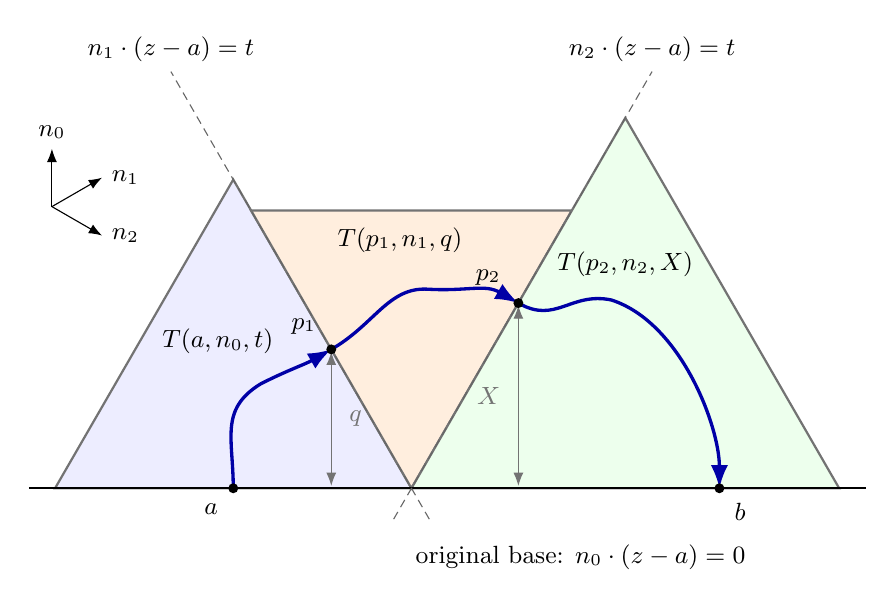
\begin{tikzpicture}[x=.98cm,y=.98cm,>=Latex,font=\small,
  region/.style={draw=black!55,thick},
  walk/.style={draw=blue!65!black,very thick},
  cut/.style={draw=black!60,densely dashed}]
  \coordinate (a) at (0,0);
  \coordinate (r) at (2.30940,0);
  \coordinate (p1) at (1.27017,1.8);
  \coordinate (p2) at (3.69504,2.4);
  \coordinate (b) at (6.3,0);

  \path[region,fill=blue!7] (-2.30940,0)--(r)--(0,4)--cycle;
  \path[region,fill=orange!13] (r)--(.23094,3.6)--(4.38786,3.6)--cycle;
  \path[region,fill=green!7] (r)--(7.85196,0)--(5.08068,4.8)--cycle;
  \draw[thick] (-2.65,0)--(8.2,0);
  \node[anchor=north] at (4.5,-.60) {original base: $n_0\cdot(z-a)=0$};

  \draw[cut] (2.54034,-.4)--(-.80829,5.4)
    node[above] {$n_1\cdot(z-a)=t$};
  \draw[cut] (2.07846,-.4)--(5.42709,5.4)
    node[above] {$n_2\cdot(z-a)=t$};

  \draw[<->,black!55,thin] (1.27017,.03)--(1.27017,1.77)
    node[midway,right=3pt] {$q$};
  \draw[<->,black!55,thin] (3.69504,.03)--(3.69504,2.37)
    node[midway,left=3pt] {$X$};

  \draw[walk,->] (a) .. controls (0,.65) and (-.18,1.02) .. (.35,1.35)
    .. controls (.68,1.52) and (.94,1.61) .. (p1);
  \draw[walk,->] (p1) .. controls (1.83,2.12) and (2.01,2.61) .. (2.52,2.58)
    .. controls (3.03,2.55) and (3.26,2.65) .. (p2);
  \draw[walk,->] (p2) .. controls (4.18,2.12) and (4.37,2.55) .. (4.9,2.44)
    .. controls (5.8,2.15) and (6.3,.8) .. (b);

  \node[align=center] at (-.2,1.9) {$T(a,n_0,t)$};
  \node[align=center] at (2.16,3.22) {$T(p_1,n_1,q)$};
  \node[align=center] at (5.08,2.9) {$T(p_2,n_2,X)$};
  \fill (a) circle (1.8pt) node[below left=2pt] {$a$};
  \fill (p1) circle (1.8pt) node[above left=2pt] {$p_1$};
  \fill (p2) circle (1.8pt) node[above left=3pt] {$p_2$};
  \fill (b) circle (1.8pt) node[below right=2pt] {$b$};
  \draw[->] (-2.35,3.65)--(-2.35,4.4) node[above] {$n_0$};
  \draw[->] (-2.35,3.65)--(-1.7,4.025) node[right] {$n_1$};
  \draw[->] (-2.35,3.65)--(-1.7,3.275) node[right] {$n_2$};
\end{tikzpicture}
\caption{The three exits producing a half-plane return from $a$ to $b$.
The depths are $q=n_0\cdot(p_1-a)$ and $X=n_0\cdot(p_2-a)$.
The first triangle lies before the first dashed line, the second lies
after that line and before the second, and the third lies after the
second line and above the original base. Thus their interiors are
disjoint, and each dashed line is crossed once by the concatenation.
The triangle boundaries have the indicated directions; the blue paths
are schematic and the lattice is omitted.}
\label{fig:geometry-three-exits}
\end{figure}


The interiors are disjoint. The second triangle satisfies
\(n_1\cdot(z-a)\ge t\), \(n_2\cdot(z-a)\le t\), while the third satisfies
\(n_2\cdot(z-a)\ge t\), \(n_0\cdot(z-a)\ge0\), and remains on or after the first line. Each of the lines \(n_1\cdot(z-a)=t\) and \(n_2\cdot(z-a)=t\) is crossed exactly once. Hence the concatenation is simple and recoverable for a fixed \(t\).

Average first over \(t\in[R,2R]\). Equation~\eqref{eq:deep-triangle-exit} retains first-exit mass \(\gtrsim R^{-1/4}\) at \(q\ge\delta R\). The second triangle then gives total two-exit mass \(\gtrsim R^{-1/2}\). The part with \(X<\eta R\) is at most
\[
 O(R^{-5/4})\sum_{\delta R\le q\le4R}\sum_{X<\eta R}k(q,X)
       \lesssim_\delta\eta R^{-1/2},
\]
by \eqref{eq:triangle-marginal} twice. Choose \(\eta>0\) small enough. The final triangle escape therefore gives averaged mass \(\gtrsim R^{-3/4}\) of these three-exit paths with \(q\ge\delta R\) and \(X\ge\eta R\).

Partition \([R,2R]\) into a fixed number of windows shorter than
\(\min(\delta,\eta)R/2\), and retain one window \(J\) with the same lower average. On the fixed measure \(\mu\) of all half-plane returns from \(a\), weighted by \(\kappa^{\ell}\), let \(E_t\) be the deep three-exit event just constructed and put
\[
 Y(\gamma)=\mathop{\mathrm{average}}_{t\in J}{\bf1}_{E_t}(\gamma).
\]
Thus \(\int Y\,d\mu\gtrsim R^{-3/4}\). If \(t<t'\) in \(J\), the simultaneous event has crossings in the order
\[
 (n_1,t),\quad(n_1,t'),\quad(n_2,t),\quad(n_2,t').
\]
Indeed the depth restrictions put \(p_1(t')\) before the \((n_2,t)\) line and \(p_2(t)\) after the \((n_1,t')\) line. Splitting at these unique crossings leaves a prefix, a middle link and a suffix, each of cost \(O(R^{-1/4})\) by triangle escape or the convex diameter bound, and two difference bridges. Therefore
\[
 \mu(E_t\cap E_{t'})\le C R^{-3/4}B_{|t-t'|/d_0}^{2},
 \qquad
 \int Y^2\,d\mu\le C R^{-5/4}.
\]
The convention \(B_0=1\) includes ties. Cauchy--Schwarz now gives
\(\mu\{Y>0\}\gtrsim R^{-1/4}\). All these returns end at a distance between fixed positive multiples of \(R\) from \(a\); monotonicity of \(K_l\) gives \(K_l\gtrsim l^{-5/4}\), completing the proof.

\end{proof}

The following confinement estimate will keep the connectors in the cylinder construction and the later sewing argument inside prescribed channels.

\begin{lemma}[Narrow-channel bridges]\label{lem:narrow-channel-bridges}
Fix an absolute constant $A$ sufficiently large. There are constants $C,R_0>0$ such that, for every strip of height $H\in d_0\mathbb Z_{>0}$ with row-boundary caps normal to one of the directions $n_j$, every starting port on one cap, and every integer $M\ge1$ with $H/M\ge R_0$, the critical mass of bridges whose transverse displacement from the starting port stays at most $4AH/M$ throughout is at least
\[
 e^{-C M} (H/M)^{-1/4}.
\]
In particular, for every fixed transverse tolerance $\tau>0$, restricting the displacement to at most $\tau H$ retains mass comparable to $H^{-1/4}$ for all sufficiently large admissible $H$, with constants allowed to depend on $\tau$.
\end{lemma}
\begin{proof}
Put \(s=H/M\). Choose the \(M-1\) internal cap levels independently in windows of length comparable to \(s\) around the equally spaced levels, so every piece has height between \(s/2\) and \(2s\). At each piece require transverse excursion at most \(A\) times its height and an endpoint shift directed towards the original axis. Reflection retains at least half the mass after the excursion restriction; the diameter tail and the two-sided strip bound make the retained mass at least \(c s^{-1/4}\) when \(A\) is large. Successive starting offsets have absolute value at most \(2As\): each shift points towards zero and has magnitude at most \(2As\). Every point of the concatenation therefore has offset at most \(4As\).

Let \(\mu\) be critical weight on bridges from the prescribed starting port between the two fixed outer caps. For a list \(\mathbf t\) of internal levels let \(E_{\mathbf t}\) be the event that the bridge has the prescribed confined pieces, and define
\[
 Y(\gamma)=\mathop{\mathrm{average}}_{\mathbf t}
           {\bf1}_{E_{\mathbf t}}(\gamma).
\]
Each level is crossed uniquely, so decomposition at a fixed list is injective and
\[
 \int Y\,d\mu\ge c^M s^{-M/4}.
\]
For two lists, split at both levels in each internal window. There are \(M\) intervening pieces of height comparable to \(s\), and \(M-1\) difference bridges within the windows. Dropping the confinement and avoidance constraints bounds the former by strip masses; averaging each latter factor \(B_{|t_i-t_i'|/d_0}\) costs at most \(Cs^{-1/4}\). Consequently
\[
 \int Y^2\,d\mu\le C^M s^{-(2M-1)/4}.
\]
This also covers \(M=1\), when there are no internal levels. Cauchy--Schwarz gives
\(\mu\{Y>0\}\ge e^{-CM}s^{-1/4}\), as claimed. For a fixed tolerance choose a fixed integer \(M\ge4A/\tau\) and combine the lower bound with the strip upper bound.

\end{proof}

\subsection{A barrier estimate on the cylinder}\label{c6:subheading-12}

Take the quotient by \(N\) horizontal lattice steps. We first construct essential polygons in slabs whose height is proportional to the period. Their positive mass will then control the vertical extent of other polygons and arches.

\begin{proposition}[Essential polygons in a slab]\label{prop:slab-essential-polygons}
There are absolute constants $c,C>0$ such that, for every sufficiently large integer $N$ and every horizontal slab $S$ of height $CN$ in the cylinder obtained by quotienting by $N$ horizontal lattice steps,
\[
 \sum_{\substack{\gamma\subset S\\ \gamma\text{ simple essential polygon}}}
       \kappa^{\ell(\gamma)}\ge c.
\]
Here essential means noncontractible in the cylinder, and the polygons are unoriented and unrooted.
\end{proposition}
\begin{proof}
Each endpoint of an arch will first exit a triangle, then cross a narrow tilted strip, and finally exit a second triangle at a common top level. We join these two endpoint collars above that level. A second moment estimate over the collar cuts gives confined arches; joining an upper and a lower arch and averaging over their base level gives the slab bound.

\paragraph{Collars.}

We give the construction with details of aperture restrictions because long-arch confinement in the periodic direction matters here. At a horizontal row boundary of level \(y_0\) in the middle region, take two midpoints \(p,q\) with horizontal separation \(D\in[N/2-\epsilon N,N/2+\epsilon N]\), \(q\) to the right in the lift. We build an arch from \(p\) to \(q\) above the line, of height \(O(N)\) and horizontal span \(<N\). The construction has symmetric independent collars at the endpoints. At \(p\):

\begin{itemize}

\item 

Exit \(T(p,n_0,s_1)\) at \(p_1\) on the side normal to \(n_1\), requiring \(n_0\cdot(p_1-p)\ge\eta N\).

\item 

Make a bridge along \(n_1\) to level \(s_2\) relative to \(p\), ending at \(p_2\), in a narrow tube transversely around the \(n_1\)-line from \(p_1\).

\item 

Exit \(T(p_2,n_1,h-n_0\cdot(p_2-p))\) at \(p_h\) on the side normal to \(n_0\) (level \(y_0+h\)). This size is half-odd in units of \(d_0\) since \(p_2\) is a midpoint in the tilted line.

\end{itemize}

Reflect these instructions at \(q\) to obtain \(q_h\). Figure~\ref{fig:geometry-collars} shows the two collars, their tilted renewal cuts and the common top line.
\begin{figure}[htbp]
\centering
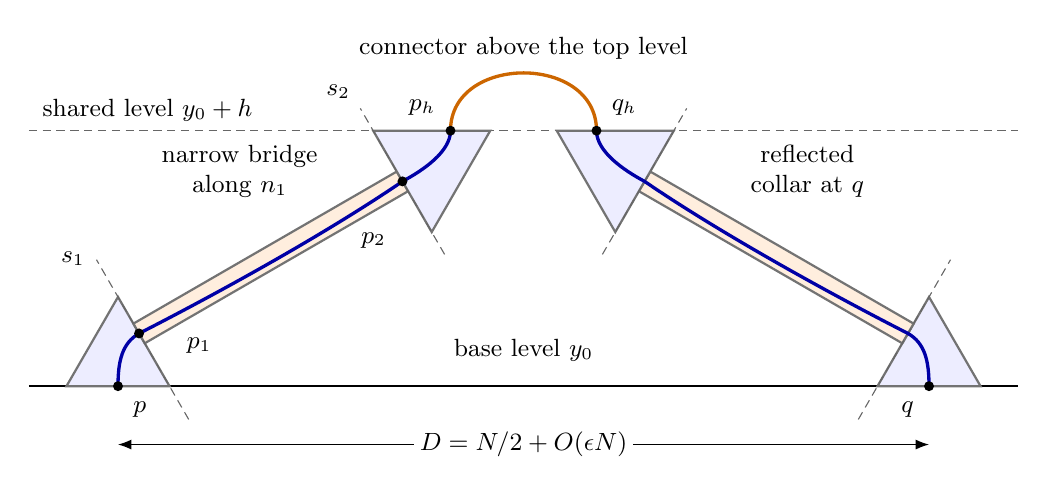
\begin{tikzpicture}[x=1.03cm,y=1.03cm,>=Latex,font=\small,
  region/.style={draw=black!55,thick},
  walk/.style={draw=blue!65!black,very thick},
  cut/.style={draw=black!60,densely dashed}]
  \draw[thick] (-1.1,0)--(11.1,0);
  \draw[cut] (-1.1,3.15)--(11.1,3.15);
  \node[anchor=west] at (-1.05,3.4) {shared level $y_0+h$};
  \node[anchor=south] at (5,.18) {base level $y_0$};

  \path[region,fill=blue!7] (-.63509,0)--(.63509,0)--(0,1.1)--cycle;
  \path[region,fill=orange!13]
    (.18981,.77124)--(.32981,.52876)--(3.57740,2.40376)
    --(3.43740,2.64624)--cycle;
  \path[region,fill=blue!7]
    (3.86824,1.9)--(3.14656,3.15)--(4.58993,3.15)--cycle;
  \draw[cut] (.87203,-.41038)--(-.26519,1.55933);
  \node[anchor=east] at (-.29,1.57) {$s_1$};
  \draw[cut] (4.02702,1.625)--(2.98778,3.425);
  \node[anchor=south east] at (2.98,3.43) {$s_2$};
  \draw[walk] (0,0) .. controls (0,.31) and (.05,.53) .. (.25981,.65)
    .. controls (1.2,1.13) and (2.55,1.87) .. (3.50740,2.525)
    .. controls (3.76,2.66) and (4.1,2.89) .. (4.1,3.15);

  \begin{scope}[xshift=10.3cm,xscale=-1]
    \path[region,fill=blue!7] (-.63509,0)--(.63509,0)--(0,1.1)--cycle;
    \path[region,fill=orange!13]
      (.18981,.77124)--(.32981,.52876)--(3.57740,2.40376)
      --(3.43740,2.64624)--cycle;
    \path[region,fill=blue!7]
      (3.86824,1.9)--(3.14656,3.15)--(4.58993,3.15)--cycle;
    \draw[cut] (.87203,-.41038)--(-.26519,1.55933);
    \draw[cut] (4.02702,1.625)--(2.98778,3.425);
    \draw[walk] (0,0) .. controls (0,.31) and (.05,.53) .. (.25981,.65)
      .. controls (1.2,1.13) and (2.55,1.87) .. (3.50740,2.525)
      .. controls (3.76,2.66) and (4.1,2.89) .. (4.1,3.15);
  \end{scope}

  \draw[very thick,orange!80!black]
    (4.1,3.15) .. controls (4.1,4.1) and (5.9,4.1) .. (5.9,3.15);
  \node at (5,4.17) {connector above the top level};
  \fill (0,0) circle (1.8pt) node[below right=2pt] {$p$};
  \fill (10,0) circle (1.8pt) node[below left=2pt] {$q$};
  \fill (.25981,.65) circle (1.8pt);
  \node at (1,.5) {$p_1$};
  \fill (3.50740,2.525) circle (1.8pt);
  \node at (3.15,1.8) {$p_2$};
  \fill (4.1,3.15) circle (1.8pt) node[above left=2pt] {$p_h$};
  \fill (5.9,3.15) circle (1.8pt) node[above right=2pt] {$q_h$};
  \node[align=center] at (1.5,2.65) {narrow bridge\\along $n_1$};
  \node[align=center] at (8.5,2.65) {reflected\\collar at $q$};
  \draw[<->] (0,-.72)--(10,-.72)
    node[midway,fill=white,inner sep=2pt] {$D=N/2+O(\epsilon N)$};
\end{tikzpicture}
\caption{The two endpoint collars and their completion, shown in the
planar lift. Each collar first exits a small triangle, crosses a narrow
tilted strip between the cuts $s_1,s_2$, and exits a final triangle at
the common height $h$. The tilted cuts are chosen independently at the
two endpoints; only $h$ is shared. The first triangles and the bridges
stay below every allowed top level, and the connector stays above the
chosen top level. These separations recover the pieces at the unique
tilted crossings and the two top crossings. Paths are schematic;
collar widths and vertical clearances are exaggerated.}
\label{fig:geometry-collars}
\end{figure}

Use the following independent windows (except that \(h\) is shared by both collars). Put \(t_*=(1/4-2\epsilon)/d_0\); choose \(s_2/N\) in a small window about \(t_*\), \(h/N\) in \(t_*/2+[0.9,1.1]\delta_h\), \(s_1/N\in[\delta_1,2\delta_1]\), on admissible levels (\(s_1,s_2\) half-odd multiples, \(h\) integer multiple of \(d_0\)). Here \(\epsilon>0\) is small, then \(\delta_h\) sufficiently small compared with \(\epsilon\); the half-width of the \(s_2/N\) window and \(\delta_1\) are both sufficiently small compared with \(\delta_h\). Choose \(\eta>0\) sufficiently small given these, and tube radius a sufficiently small fixed multiple of \(N\) compared with \(\eta N\).

Thus the bridge after the deep exit stays above \(y_0\), and both it and the first triangle stay below the lowest available top level \(y_0+h_{\min}\) by a margin comparable to \(\delta_h N\). Indeed before the last triangle the maximal vertical rise from \(p\) is at most \(s_2/2+O(\delta_1 N+\text{tube radius})\), and \(p_2\)'s height is within this error of \(y_0+s_2/2\). The left collar has horizontal displacements from \(p\) between \(-O(\delta_h N)\) and \((1/4-2\epsilon)N+O(\delta_h N)\), the endpoint near the latter within \(O(\delta_h N)\), by \(n_1=(d_0,1/2)\); similarly on the right. Thus collars are separated, themselves simple by the transversal renewals, and each last triangle still stays strictly above the base (its diameter is \(O(\delta_h N)\)), and terminal horizontal separation is in \([\epsilon N,7\epsilon N]\).

\paragraph{Completion.}
Complete by a half-plane arch joining \(p_h,q_h\) above, with diameter \(\le N/10\). This has no unwanted contacts and the whole arch projects simply.

Averaged over the parameters the product mass \(M_0\) of collars before completion is \(\gtrsim N^{-6/4}\): for each, the averaged deep first exit is \eqref{eq:deep-triangle-exit}, the narrow bridge is supplied by Lemma~\ref{lem:narrow-channel-bridges}, and the last triangle uses \eqref{eq:triangle-escape}. This mass is independent of \(D\).

Without truncating the connector diameter, the sum of product weights including the connector is at least \(c_0(\epsilon N)^{-5/4}M_0\) for each \(D\), with absolute \(c_0>0\), by \(K_l\). The loss by truncation, summed over the integer \(D\)'s, is at most \(C_0 N^{-1/4} M_0\), also with an absolute constant, since for fixed collars varying \(D\) just translates the right endpoint, and we have the completed-path diameter bound. Hence for \(\epsilon\) chosen sufficiently small, at least three quarters of the choices of \(D\) retain averaged mass \(\gtrsim N^{-11/4}\). The concatenation (truncated) is injective for fixed parameters: the top level is crossed precisely twice and on each collar the tilted levels have unique crossings.

\paragraph{Second moment over collar cuts.}
Fix one of the retained separations \(D\) and the endpoints \(p,q\). Let \(\mu_{p,q}\) be critical weight on all simple half-plane arches from \(p\) to \(q\). A cut list is
\(\vartheta=(s_1^p,s_2^p,s_1^q,s_2^q,h)\), with the five independent window laws above. Write \(E_\vartheta\) for the event that an arch admits the prescribed collar decomposition and truncated connector, and set
\[
 Y(\gamma)=\mathop{\mathrm{average}}_\vartheta
            {\bf1}_{E_\vartheta}(\gamma).
\]
The recovery observation gives \(\int Y\,d\mu_{p,q}\gtrsim N^{-11/4}\). To bound its second moment, compare two lists on this same arch measure. Their joint mass is at most
\[
 C N^{-11/4} B_{|h-h'|/d_0}^2
 \prod_{\rm both\ collars} B_{|s_1-s'_1|/d_0}\, B_{|s_2-s'_2|/d_0}.
\]
In fact before the first crossing of the lower of the two top levels, both tilted levels of each list on the \(p\) collar were already crossed uniquely (they are reached strictly below all possible top levels, in the first two pieces, then not crossed again on the collar). Thus chronologically split at these four tilted lines. Prefix to the lowest costs \(O(N^{-1/4})\); from the larger first to the smaller second another \(O(N^{-1/4})\); from the largest to the lower top level, start with normal \(n_1\) and end with normal \(n_0\) within the convex wedge on the proper side of both lines, costing \(O(N^{-1/4})\) by the diameter bound (vertical gap \(\gtrsim N\)). The small intervening bridges yield the indicated difference factors.

Similarly split from \(q\), leaving two vertical bridges of gap \(|h-h'|\) and a top connector bounded by \(K_l=O(N^{-5/4})\) using endpoint separation for the higher-top choice. This proves the bound including ties. Each of the four tilted difference factors averages to \(O(N^{-1/4})\); the shared top-level pair averages to \(O(N^{-1/2})\). Thus
\[
 \int Y^2\,d\mu_{p,q}\le C N^{-17/4},
 \qquad
 \mu_{p,q}\{Y>0\}\ge
 \frac{(\int Y\,d\mu_{p,q})^2}{\int Y^2\,d\mu_{p,q}}
 \gtrsim N^{-5/4}.
\]
This is the confined arch mass on each retained choice of \(D\).

\paragraph{Slab barrier.}
The confined arches can now be joined across a base level and averaged over that level. At least three quarters of the choices of \(D\) are retained for the upper arch. The same holds, after \(D\mapsto N-D\), for the lower arch joining \(q\) to \(p+N\). Their intersection therefore contains a positive fraction of all choices. Joining and projecting, summing over both points with at most bounded overcount, gives mass \(\gtrsim N^{-1/2}\) for polygons crossing the specified \(y_0\) exactly twice at such separated points and staying in our slab.

Let \(\nu\) be critical weight on unoriented unrooted simple essential polygons in the fixed slab. For a base level \(y_0\) in the middle window, let \(F_{y_0}\) be the event just constructed, including its upper and lower arch restrictions. We have \(\nu(F_{y_0})\gtrsim N^{-1/2}\). For two levels \(y_0,y'_0\) the joint mass is \(\lesssim N^{-1/2} B_{|y_0-y'_0|/d_0}^2\): split into upper and lower arches at the higher and lower levels respectively (each costing \(O(N^{-5/4})\) with endpoints given), and two intervening bridges, summing over \(O(N^2)\) endpoint pairs on one level and then bounding bridges separately with other ends free. Each simple arch in the cylinder lifts with endpoint displacement at most \(N\) (larger gives interleaving and intersection with its translate), so has at most two endpoint choices given the start and projected end. For \(Y_0=\mathop{\mathrm{average}}_{y_0}{\bf1}_{F_{y_0}}\), averaging over the window of order \(N\) therefore gives
\[
 \int Y_0\,d\nu\gtrsim N^{-1/2},\qquad
 \int Y_0^2\,d\nu\lesssim N^{-1}.
\]
Cauchy--Schwarz yields \(\nu\{Y_0>0\}\gtrsim1\), proving the slab bound.

\end{proof}

\paragraph{Positivity of the negative polymer polynomial.}
We next obtain a partition-function comparison that turns the slab mass into a penalty for large height. The positivity statement below holds for every integer period, including the smallest ones. Let $D$ be the finite cylinder between horizontal row-boundary caps. Write its height as $H=h d_0$, with $h\ge1$ an integer, and retain distinct edges in the quotient by $N\ge1$ horizontal lattice steps. A simple polygon is an embedded closed curve in this cylinder; it may therefore have two edges when the quotient has parallel edges. Let $\mathcal P$ be the finite set of these polygons. For $0\le\beta'\le3/8$, put
\[
 \alpha=\pi\beta'/3,\qquad x=(2\cos\alpha)^{-1},\qquad
 \omega(L)=x^{|L|}\begin{cases}
 -2\cos(4\alpha),&L\text{ contractible},\\
 -2\cos(2\alpha),&L\text{ essential}.
 \end{cases}
\]
For every $\mathcal A\subseteq\mathcal P$, define
\[
 Q(\mathcal A)=\sum_{\substack{\mathcal F\subseteq\mathcal A\\
                         \text{polygons in }\mathcal F\text{ mutually disjoint}}}
                  \prod_{L\in\mathcal F}\omega(L).
\]
The empty system contributes $1$. We will use positivity not only for the full cylinder but for every set of available polygons.

\begin{auxproposition}[Positivity on all polygon subsets]
For every integer period $N\ge1$, every finite height $h\ge1$, every $0\le\beta'\le3/8$, and every $\mathcal A\subseteq\mathcal P$, the polynomial above satisfies $Q(\mathcal A)>0$.
\end{auxproposition}
\begin{proof}

We first describe the quotient at the short periods. After a lattice translation put the bottom cap at level zero. Set $a=(1,0)$ and $b=(1/2,d_0)$, and denote the centers of the triangles
\[
 \begin{split}
 U_{i,j}&=[ia+jb,(i+1)a+jb,ia+(j+1)b],\\
 D_{i,j}&=[(i+1)a+jb,ia+(j+1)b,(i+1)a+(j+1)b]
 \end{split}
\]
by the same letters. Here $i$ is taken modulo $N$ and $0\le j<h$. The links inside row $j$ are $U_{i,j}D_{i,j}$ and $D_{i,j}U_{i+1,j}$; the links between rows are $D_{i,j}U_{i,j+1}$ for $j<h-1$.

If $N=1$, the two links in each row are distinct parallel edges between its two centers. Each link between rows is a bridge of the finite graph, so no polygon uses it. Consequently the only polygons are the $h$ mutually disjoint essential two-edge row cycles. For any subset $\mathcal A$,
\[
 Q(\mathcal A)=\bigl(1-2\cos(2\alpha)x^2\bigr)^{|\mathcal A|}
             =\left(\frac1{2\cos^2\alpha}\right)^{|\mathcal A|}>0.
\]
This proves the assertion at period one, including both parameter endpoints.

If $h=1$ at any period $N$, the graph is just one essential $2N$-edge row cycle. The only nonempty polymer subset therefore has polynomial
\[
 1-2\cos(2\alpha)x^{2N}\ge 1-2\cos(2\alpha)x^2
 =\frac1{2\cos^2\alpha}>0,
\]
since $0<x\le\kappa<1$ and $\cos(2\alpha)>0$.

Suppose henceforth that $N,h\ge2$. The elementary polygon about the interior lattice point $ia+jb$, $1\le j<h$, has successive centers
\[
 U_{i,j},\ D_{i-1,j},\ U_{i-1,j},\ D_{i-1,j-1},\ U_{i,j-1},\ D_{i,j-1}.
\]
These six centers are distinct modulo $N$, even when $N=2$. The polygon and its enclosed disk have horizontal width $1<N$, so their projection is embedded and contractible. Elementary polygons about adjacent points on an interior horizontal row share centers, and those about $ia+jb$ and $ia+(j+1)b$ share centers when both exist. They therefore form a connected overlap family. Every triangle in the cylinder has a corner on an interior row because $h\ge2$, so every polygon meets at least one member of this family. Thus the incompatibility graph of all polygons, in which two polygons are adjacent when they share a center, is connected for every $N\ge2$.

We recall the flux identity with detached polygons. Start at a bottom boundary port $p$ and assign a path the phase $e^{i\beta' W}$, where $W$ is its total turn. At a previously unvisited center the two outgoing turns are $\pm\pi/3$, and $2x\cos\alpha=1$. If an incoming prefix returns to a center previously reached by a stem, pair the two orientations of the unfinished loop there. They cancel the term stopped at the stem with the corresponding detached polygon occupying that center. The incremental turns from the stem are $\pm4\pi/3$ for a contractible loop, whose source is outside, and $\pm2\pi/3$ for an essential loop. To see the latter value, an essential simple loop has total turn zero in flat cylinder coordinates: under the exponential map to the punctured plane its Jordan-curve turn $\pm2\pi$ is supplied by the winding of the frame. In either case subtract twice the closing turn at the center from the loop's total turn, since departure from the stem turns oppositely. This gives exactly the two cosine factors in $\omega(L)$.

Summing these cancellations gives the signed exit identity
\[
 Q(\mathcal P)=\sum_{\gamma:\,p\to\partial D}
 x^{|\gamma|}e^{i\beta'W(\gamma)}
 Q\bigl(\{L\in\mathcal P:L\cap\gamma=\varnothing\}\bigr).
\]
Here paths stop at their first boundary exit, and length counts visited centers. The real coefficients of all path terms are positive: lifted bridges have turn $0$, and lifted same-cap arches have turn $\pm\pi$. At $\beta'=0$ and $0\le x\le1/2$, the same calculation includes additional defect terms on the right, each with factor $1-2x$ times an incoming prefix weight and the polynomial of its available detached polygons. These terms are nonnegative whenever all subset polynomials are nonnegative.

Continue first from $x=0$ to $x=1/2$ at $\beta'=0$, and then along the critical parameters up to but excluding $\beta'=3/8$. If some subset polynomial first became zero, all subset polynomials would be nonnegative at that parameter. Choose an inclusion-minimal zero subset $\mathcal A$. It is nonempty and all its proper subset polynomials are positive. Every individual polygon weight is strictly negative at this first zero. If $L\notin\mathcal A$ conflicts with some member of $\mathcal A$, the deletion identity gives
\[
 Q(\mathcal A\cup\{L\})
 =Q(\mathcal A)+\omega(L)Q\bigl(\mathcal A\setminus\mathcal N(L)\bigr)<0,
\]
where $\mathcal N(L)$ is the set of polygons meeting $L$. Connectedness of the incompatibility graph therefore forces $\mathcal A=\mathcal P$. In the real flux identity all terms are then nonnegative. A bridge obtained by successively visiting $U_{i,j},D_{i,j}$ in every row has positive weight and deletes at least one elementary polygon. Its residual polynomial is a proper-subset polynomial and hence positive, contradicting $Q(\mathcal P)=0$.

At $\beta'=3/8$, all subset polynomials are nonnegative by continuity, contractible polygon weights are zero, and essential polygon weights are $-\sqrt2\kappa^{|L|}$. Adding a polygon can only decrease a subset polynomial, by the same deletion identity. Thus a zero subset would force $Q(\mathcal P)=0$. In the real flux identity the displayed bridge excludes every essential polygon by separation of the two caps. Its residual polynomial is exactly $1$, since the remaining contractible polygons have zero weight. Its strictly positive contribution again contradicts $Q(\mathcal P)=0$. This completes the proof of strict positivity at every period and on the entire closed interval.
\end{proof}

\paragraph{Deletion ratios and the free-energy bound.}
With positivity on all subsets established, we compare the full partition with the partition obtained by deleting polygons that hit a given path or polygon. At the endpoint parameters let \(Z_H(t)\) use essential polygons only, with factor \(-t\), \(0\le t\le\sqrt2\). Positivity for all subsets continues to hold by multiaffinity (average over deletions). If \(H_H(\gamma;t)\) denotes the polynomial restricted to polymers not hitting \(\gamma\), divided by \(Z_H(t)\), then the following bound measures the cost of the deletion:
\begin{equation}\label{eq:cylinder-deletion-ratio}
 H_H(\gamma;t)\ge\exp\left(t\sum_{\ell\ \mathrm{essential},\ \ell\cap\gamma\ne\varnothing}
                 \kappa^{|\ell|}\right).
\end{equation}
Indeed insert the missing polymers one by one; at each insertion the polynomial decreases by \(t\kappa^{|\ell|}\) times a compatible subpartition, at least \(t\kappa^{|\ell|}\) times the current polynomial, by positivity on all subsets. With one starting point at the bottom the real flux identity becomes
\[
 1=B^{\rm cy}_H/Z_H(\sqrt2)+ c\sum_{\gamma\ \mathrm{arch}}\kappa^{|\gamma|} H_H(\gamma;\sqrt2)
\]
where \(B^{\rm cy}_H\) sums cylinder bridges. For \(H\ge N\), the arch part includes ordinary base returns in a small centered triangle of size comparable to \(N\), so \(B^{\rm cy}_H/Z_H\lesssim N^{-1/4}\) by \(S\).

The bridges themselves have mass at least \(e^{-C H/N}N^{-1/4}\) by Lemma~\ref{lem:narrow-channel-bridges} with \(M\) of order \(H/N\) chosen to fit strictly inside the period. Therefore
\begin{equation}\label{eq:cylinder-free-energy}
 -\log Z_H(\sqrt2)\le CH/N,\qquad H\ge N.
\end{equation}

For the bounded set of periods below the threshold needed by the narrow-channel construction, the explicit bridge above gives $Z_H(\sqrt2)\ge\kappa^{2h}$ when $N,h\ge2$. The same inequality for $N=1$ or $h=1$ follows directly from the displayed row-cycle formulas. Thus the same bound $-\log Z_H(\sqrt2)\le CH/N$ holds after enlarging the absolute constant. The endpoint positivity and deletion monotonicity give the same upper bound for $-\log Z_H(t)$ when $0\le t\le\sqrt2$.

Differentiation gives
\begin{equation}\label{eq:cylinder-integrated-ratio}
 \int_1^{\sqrt2}\sum_{\ell\ \mathrm{essential}}\kappa^{|\ell|}H_H(\ell;t)\,dt
 \le C H/N.
\end{equation}
\paragraph{Height tails.}
The bounded periods also have a uniform slab lower bound: each triangular strip contains the essential $2N$-edge row cycle, of weight $\kappa^{2N}$, whose minimum over these finitely many periods is positive. Taking the slab-height constant large enough to contain a full triangular strip therefore extends the barrier lower bound to them. Consequently the following height estimates use constants independent of the period.

The following consequences will be used in the nesting comparison. They also hold in either other lattice-axis orientation.
\begin{auxproposition}[Cylinder barriers and height tails]
On the infinite cylinder of period $N$, the individual critical weights of essential polygons meeting a fixed horizontal level have bounded sum. From a fixed bottom port in a semi-infinite cylinder, arches reaching height $s$ have mass at most $Ce^{-cs/N}$. For $s\ge1$, all polygons meeting a fixed level and with height span in $[s,2s]$ have total mass at most $\operatorname{poly}(N,s)e^{-cs/N}$, with a fixed polynomial bound.
\end{auxproposition}
\begin{proof}
We combine \eqref{eq:cylinder-deletion-ratio} with Proposition~\ref{prop:slab-essential-polygons} to control vertical span. An essential polygon with vertical height span \(s\), or an arch from the bottom reaching up by \(s\), must hit all short essential polygons in each slab completely traversed. Using order \(s/(CN)\) disjoint slabs and the slab mass bound gives \(H_H(\gamma;t)\gtrsim \exp(c' s/N)\) for \(t\ge1\), \(c'>0\).

Consequently the unadorned mass of essential polygons meeting a given horizontal line on the infinite cylinder is \(O(1)\): sum by spans between \(jN,(j+1)N\), each time using a containing cylinder of height \(O((j+1)N)\) and the last integral bound. The unadorned arch mass from a fixed base midpoint reaching \(s\) in a semi-infinite cylinder is \(\lesssim e^{-c' s/N}\) by the arch flux bound and exhaustion.

We explain also the height-tail bound for unmarked polygons. For $N\ge3$ a polygon of large height can be opened into such an arch at the bottom of its lowest occupied triangle row by bounded-cost surgery.

In that row an upward triangle center \(v\) must occur (any downward triangle there needs a tilted connection to such a center), using both tilted neighbors \(w_\pm\). If one such neighbor uses its other tilted connection to another upward center \(u\), cut that segment \(v,w,u\) (remove \(w\)) and attach \(v,u\) to the base line directly.

Otherwise both neighbors continue north and the upward centers across their other tilted connections are unoccupied (being occupied would force both slants there). Remove \(v\) and attach \(w_\pm\) to the base via these free centers.

In either case the surgery yields a simple arch, still reaching within bounded distance of the same height, with bounded multiplicity given the local surgery site.

For $N=2$, every polygon occupying more than one triangular strip uses exactly one of the two upward centers in its lowest strip. Indeed both upward centers would each have to use both tilted links, forcing the polygon to be the four-edge row cycle. Thus both downward centers are used and continue into the next strip, while the other upward center is unoccupied. Replace the two-link segment through the occupied upward center by the two-link segment through the other one. This gives a simple polygon of the same length and exactly the same minimum and maximum heights. The two alternative segments together form the essential four-edge row cycle, so the replacement changes the winding number by $1$ or $-1$ and takes a contractible polygon to an essential one. The operation is an involution, recovered from the lowest strip, and hence is injective. The already established essential-polygon tail therefore bounds these contractible polygons as well. At $N=1$ every polygon is a row digon and has bounded height span. These two cases complete the height-tail argument at the remaining periods.

Thus polygons meeting a given level with span between \(s\) and \(2s\) have mass \(\le\operatorname{poly}(N,s)e^{-c' s/N}\), by summing arch bounds and surgery locations. Rotation gives the same argument in either other lattice-axis orientation.
\end{proof}
These tails allow the nesting comparison in the next subsection to discard separators with excessive vertical or horizontal span.

\subsection{Passing to local nesting and bulk length}\label{c6:subheading-13}

In the plane let \(Z(R)\) be the positive partition function (including empty) of mutually disjoint simple polygons surrounding a given triangular lattice point, within radius \(R\) of it, factor 2 per polygon, activity \(\kappa^{\rm length}\). We claim
\[
 Z(R)=R^{1/12+o(1)}.
\]
Indeed on the even cylinder with antipodal marked points on the same level we computed \(\mathcal Z=N^{1/6+o(1)}\) for factor 2 on separating polygons. It bounds \(Z(c_1 N)^2\) above for sufficiently small \(c_1>0\) (that is, \(\mathcal Z\ge Z(c_1 N)^2\)). Conversely we can disregard essential polygons at bounded multiplicative cost in an upper bound for \(\mathcal Z\), since they must meet the joining segment and the sum of their single-loop weights is bounded. A contractible separator lifts uniquely around a specified preimage of the marked point on its inside, by simplicity (translated lifts have disjoint interiors). Hence its vertical extent straddles the common level. Those with vertical span above \(N^{1+\xi}\), for any fixed \(\xi>0\), are negligible in individual weight sum by the height tail. For the rest, if horizontal span in the lift exceeds \(N^{1+2\xi}\), project the specified lift around its marked point instead onto a cylinder tilted by \(60^\circ\) with integer period length between \(4 N^{1+\xi}\) and \(5 N^{1+\xi}\). It projects injectively even including the disk inside, by its narrow vertical span, and can be recovered from this polygon by the mark; it meets the level there of the mark and its span normal to the new period is of order at least \(N^{1+2\xi}\). The same height tail discards these as well. Disregarding all discarded polygons costs at most the exponential of twice the sum of their individual weights. All others split into the two types by the point inside, lifting to disjoint plane polygons within each type and supported up to radius \(C N^{1+2\xi}\); systems inject accordingly. Thus
\(
 \mathcal Z\lesssim Z(C N^{1+2\xi})^2
\).
Both comparisons, monotonicity and then \(\xi\downarrow0\) give the claim.

\begin{proposition}[Boundary occupancy]\label{prop:occupancy}
Let $D$ be a finite convex tiled domain and let $e$ be an internal honeycomb link crossing a tiling edge $[y,z]$. If $U_D(e)$ is the critical mass of paths using $e$ with ordered free boundary ports, and $Z_D(y),Z_D(z)$ are the positive enclosing-polygon partitions with factor $2$, then
\[U_D(e)\asymp Z_D(y)+Z_D(z).\]
The comparison constants are absolute.\end{proposition}
\begin{proof}
We compare the two enclosing-polygon partitions with a signed exit sum from the cut link, then recover the complete chords using that link.

\paragraph{Cut-link identity.}
Let \(D\) be a finite convex tiled domain, \(e\) an interior link (identified with the midpoint of a tiling edge \([y,z]\)). Cut \(e\), producing two boundary ends at the same midpoint. Let \(Z_e\) count detached systems of pairwise disjoint simple polygons in this cut domain surrounding that midpoint, factor 2 and critical weight as above. For either choice of cut end as source, the total signed exit mass to the \emph{outer} boundary in the cut domain has real part
\[
 S_e= Z_e+\tfrac1{\sqrt2}(M_y+M_z).
\]
Here \(M_y\) sums a polygon using \(e\) (unoriented, weight without factor 2), having \(y\) inside, together with an exterior system of detached polygons as for \(Z_e\), avoiding that polygon; and similarly for \(M_z\).

Indeed transport prefix flux \(\kappa^{|\eta|}\exp(i\beta W(\eta))\) from this source with any disjoint detached polygons of the specified kind allowed. At a free next triangle center, not previously visited and not occupied by a detached polygon, the two continuations conserve flux with these same polygons. Incoming prefixes returning toward a previously visited center pair by reversing the unfinished polygon there, going back to the first visit. Their turn increments beyond the incoming stem before first visit are total turn of the polygon minus twice its closing turn there (the departure from the stem turns oppositely instead). Thus they are \(\pm4\pi/3\) if the stem came from outside (closing turns convex), \(\pm8\pi/3\) if from inside (closing turns concave); indeed the stem is attached along the unique unused ray and cannot intersect the polygon, so its side is determined by whether the polygon surrounds the cut source. The phases sum to zero outside, and inside both equal \(-1\), canceling the term with the prefix stopped at the incoming stem and that same polygon detached instead, of relative weight 2 times the polygon weight. This partitions the blocked arrivals (at previously visited centers or centers occupied by detached polygons), establishing the exit identity with initial value \(Z_e\). Paths to the outer boundary admit no detached polygons by separation. The other exits end at the opposite cut end and close a polygon once with turn \(\pm2\pi\), real phase \(-1/\sqrt2\) and allowed detached systems necessarily exterior to it. This proves the formula. Also the centered partition functions at \(y,z\) in \(D\) are respectively \(Z_D(y)=Z_e+2M_y,\ Z_D(z)=Z_e+2M_z\) by testing crossings of \([y,z]\). Indeed disjoint polygons about \(y\) either all avoid \(e\), hence all surround the midpoint, or just one uses it (the only possible crossing of this segment), and this one must be innermost since it encloses \(y\) but not \(z\).

\paragraph{Recovering complete chords.}
For an ordinary outer source \(a\), in the cut domain \emph{without} detached loops the same contour works with initial value 1 (stem never inside). Subtract the uncut exit identity to see that the signed mass of complete outer paths from \(a\) using \(e\) equals the signed exit to the cut ends. Summing over all boundary sources and reversing these prefixes, the real mass becomes \(2S_e\). All real weights on complete chords are comparable to unsigned ones. Consequently for free boundary endpoints the unsigned mass of complete paths using \(e\) satisfies
\[
 U_D(e)\asymp Z_D(y)+Z_D(z)
\]
with absolute constants.
\end{proof}

The bounded-factor nesting estimate in the next section will turn this identity into the sharp first-length mass used in the exterior sewing argument.

\section{Bounded-factor nesting estimates}\label{sec:uniform-nesting}

The exponent-level saturation proved above identifies a nonzero normalization. We now strengthen both the comparison between plane and cylinder and the analytic estimate. The first removes large polygons at bounded cost; the second proves convergence of the normalized edge contributions. Together they prove the first assertion of Theorem~\ref{thm:nesting}.

\subsection{Uniform geometric comparison}\label{c6:uniform-geometry}

The height tails of the preceding section discard polygons much larger than the period, but their polynomial prefactor does not yet give a bounded cost at scale $N$. We first bound the individual polygon mass in each planar diameter annulus. A refinement of the cylinder free-energy estimate will then leave only a uniformly bounded number of exceptional annuli.

Keep $\beta=3/8$. Let $D$ be a finite cylinder between flat caps, or a finite convex tiled polygon in the plane. Write $Q_D=Z_H(\sqrt2)$ in the cylinder and $Q_D=1$ in the plane, and use the same notation for restrictions of the available essential polygons. All these polynomials are positive. For a set $K$ of occupied centers put
\[
 H_D(K)=Q_{D\setminus K}/Q_D,
\]
where the numerator removes the essential polygons hitting $K$. These ratios increase as the available polygon set grows. Indeed, for one deleted polygon $v$ in a set $P$,
\[
 \frac{Q_P}{Q_{P\setminus v}}
 =1-t\kappa^{|v|}\frac{Q_{P\setminus N[v]}}{Q_{P\setminus v}},
\]
where $N[v]$ is its closed conflict neighborhood. Induction on $|P|$, deleting its neighbors successively in the smaller set, gives the claim; extra neighbors only increase the deletion ratio. Products give the assertion for several deletions. The same reasoning applies for $0\le t\le\sqrt2$.

Write $\mathcal Y(y)$ for the partition with these essential polygons and, in addition, mutually disjoint contractible polygons enclosing the triangular lattice vertex $y$, each with factor $2$. Expanding in the enclosing polygons leaves positive restricted essential partitions, so $\mathcal Y(y)\ge Q_D$, including when $y$ lies on a cap.

For a simple polygon $L\subset D$ and a boundary source $a$, let $P(a,L)$ be the real part of the normalized signed mass of stems first hitting $L$. Stop a stem at the incoming midpoint before visiting its first center of $L$; include all essential polygons disjoint from the stem and $L$, and divide by $Q_{D\setminus L}$. The contour identity identifies this with $1$ minus the real normalized mass exiting to the original boundary in the domain with $L$ removed. This convention gives $P(a,L)=1$ if the first center towards which $a$ points has been removed. Since outer-exit real phases are positive and the deletion ratios increase before removal,
\begin{equation}\label{eq:first-hit-comparison}
 1\ge P(a,L)\ge
 \sum_{\substack{\gamma:\,a\to\partial D\\\gamma\cap L\ne\varnothing}}
 \kappa^{|\gamma|}\cos(\beta W(\gamma))H_D(\gamma)\ge0.
\end{equation}

\begin{auxlemma}[A primitive of the boundary flux]
Choose a dual-edge chain $\Gamma$ from a boundary lattice vertex $y_0$ to an interior lattice vertex $y$. For an oriented honeycomb link, count a crossing of $\Gamma$ positively when the chain goes from its right face to its left face. Let $\operatorname{cr}_\Gamma(\gamma)$ be the sum of these signs along a completed path and set
\[
 I=\Im\sum_{a\in\partial D}\sum_{\gamma:\,a\to\partial D}
   \operatorname{cr}_\Gamma(\gamma)\,
   \kappa^{|\gamma|}e^{i\beta W(\gamma)}H_D(\gamma).
\]
The sum over $a$ is over all ordinary boundary ports. Then
\begin{equation}
 2\!\!\sum_{L\text{ contractible enclosing }y}
       \kappa^{|L|}H_D(L)\sum_aP(a,L)
 \le |I|+\sqrt2\!\sum_{L\text{ essential}}
       \kappa^{|L|}H_D(L)\sum_aP(a,L).
 \label{eq:legacy-P-G1}
\end{equation}
The essential sum is absent in the plane.
\end{auxlemma}
\begin{proof}
We compute the same prefix current in two ways. For a prefix $\eta$ from $a$ to an oriented internal-link midpoint $e$, write $\epsilon_\Gamma(e)$ for the crossing sign just specified, or zero if the chain does not cross $e$. Define
\[
 J=\Im\sum_{a\in\partial D}\sum_{e,\eta:\,a\to e}
     \epsilon_\Gamma(e)\,
     \kappa^{|\eta|}e^{i\beta W(\eta)}H_D(\eta).
\]
Only centers already visited by $\eta$ are deleted in $H_D(\eta)$. Repeated chain crossings, if present, are counted with their signed multiplicities. Figure~\ref{fig:geometry-current} records the orientation convention.
\begin{figure}[htbp]
\centering
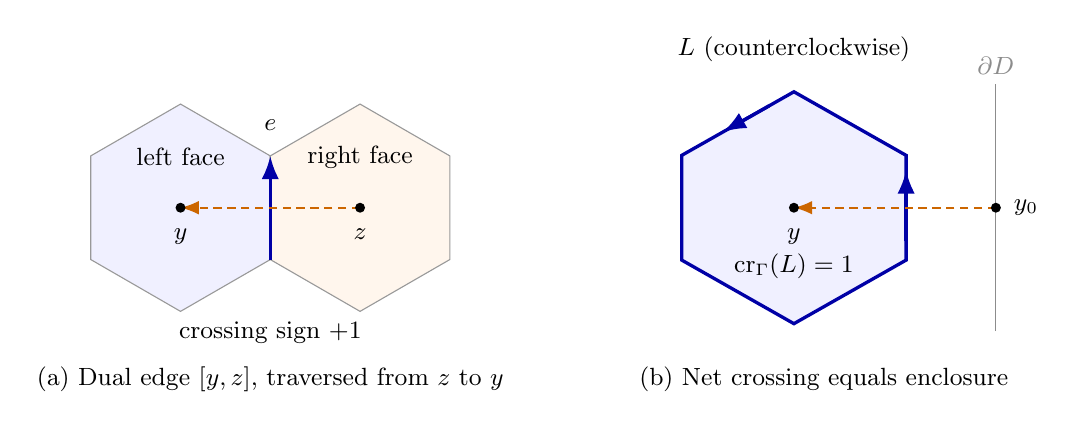
\begin{tikzpicture}[x=.95cm,y=.95cm,>=Latex,font=\small,
  primal/.style={draw=blue!65!black,very thick},
  dual/.style={draw=orange!80!black,thick,densely dashed}]
  \path[draw=black!40,fill=blue!6]
    (0,-.69282)--(0,.69282)--(-1.2,1.38564)--(-2.4,.69282)
    --(-2.4,-.69282)--(-1.2,-1.38564)--cycle;
  \path[draw=black!40,fill=orange!7]
    (0,-.69282)--(1.2,-1.38564)--(2.4,-.69282)--(2.4,.69282)
    --(1.2,1.38564)--(0,.69282)--cycle;
  \draw[primal,->] (0,-.69282)--(0,.69282);
  \node[anchor=south] at (0,.90) {$e$};
  \draw[dual,->] (1.2,0)--(-1.2,0);
  \fill (-1.2,0) circle (1.8pt) node[below=4pt] {$y$};
  \fill (1.2,0) circle (1.8pt) node[below=4pt] {$z$};
  \node at (-1.2,.68) {left face};
  \node at (1.2,.68) {right face};
  \node at (0,-1.67) {crossing sign $+1$};
  \node at (0,-2.3) {(a) Dual edge $[y,z]$, traversed from $z$ to $y$};

  \begin{scope}[xshift=6.65cm]
    \path[fill=blue!6]
      (1.5,-.7)--(1.5,.7)--(0,1.55)--(-1.5,.7)
      --(-1.5,-.7)--(0,-1.55)--cycle;
    \draw[primal]
      (1.5,-.7)--(1.5,.7)--(0,1.55)--(-1.5,.7)
      --(-1.5,-.7)--(0,-1.55)--cycle;
    \draw[primal,->] (1.5,-.45)--(1.5,.5);
    \draw[primal,->] (-.33,1.363)--(-.95,1.012);
    \node[anchor=south] at (0,1.82) {$L$ (counterclockwise)};
    \draw[black!45] (2.7,-1.65)--(2.7,1.65)
      node[above] {$\partial D$};
    \draw[dual,->] (2.7,0)--(0,0);
    \fill (2.7,0) circle (1.8pt) node[right=3pt] {$y_0$};
    \fill (0,0) circle (1.8pt) node[below=4pt] {$y$};
    \node at (0,-.78) {$\operatorname{cr}_\Gamma(L)=1$};
    \node at (.4,-2.3) {(b) Net crossing equals enclosure};
  \end{scope}
\end{tikzpicture}
\caption{The crossing convention for the current primitive.
(a) The oriented honeycomb link $e$ crosses the tiling edge $[y,z]$;
the dual traversal from its right face to its left face has sign $+1$.
Reversing either orientation reverses this sign.
(b) For a counterclockwise contractible polygon, the interior lies to
the left. Hence a dual chain from the exterior boundary gap $y_0$ to
$y$ has net crossing $1$ if the polygon encloses $y$, and $0$ otherwise.
The global polygon and chain are schematic. These are topological
crossing signs; the imaginary prefix-current coefficient is computed
separately in the proof.}
\label{fig:geometry-current}
\end{figure}


\paragraph{Reverse at the cut link.}
Reverse the prefixes ending at $e$ and apply the cut-link calculation from Proposition~\ref{prop:occupancy}. Permit contractible detached polygons about the cut midpoint with factor $2$, and retain the essential detached polygons. The essential blocked-loop turns are still $\pm2\pi/3$, irrespective of the stem side, so their cancellation is unchanged. A return through the cut along an essential polygon has turn zero. A contractible return has turn $\pm2\pi$; reversal conjugates the phase and exchanges the two link directions. Thus the imaginary current across a dual edge is $-1/\sqrt2$ times the left-minus-right difference of the centered partitions, divided by $Q_D$. Each enclosing polygon crossing that dual edge is counted once with its factor $2$. Along outer exits from the cut no enclosing contractible polygon remains. Telescoping from $y_0$ to $y$ therefore gives
\begin{equation}\label{eq:prefix-current-potential}
 J=-\frac{\mathcal Y(y)/Q_D-1}{\sqrt2}.
\end{equation}
Here $\mathcal Y(y_0)=Q_D$ because a contractible polygon in $D$ cannot enclose a boundary vertex.

\paragraph{Continue the prefixes.}
Instead continue each prefix to its first exit, treating its past centers as additional deleted boundary. The starting residual partition is exactly the one already attached to the prefix. A loop in this continuation cannot surround its source, which remains accessible along the past. The exits are either completed boundary paths, giving $I$, or blocked returns to a past center. Each blocked return consists uniquely of a first-hitting stem followed by an incomplete simple polygon; all detached polygons avoid both pieces.

Pair the two orientations of this polygon, including their opposite link-crossing signs. The coefficients of their circulation are
\[
\begin{array}{c|c|c}
 \text{polygon}&\text{additional turns}&\text{oriented phase difference}\\ \hline
 \text{contractible}&\pm4\pi/3&e^{i\pi/2}-e^{-i\pi/2}=2i\\
 \text{essential}&\pm2\pi/3&\pm(e^{i\pi/4}-e^{-i\pi/4})=\pm i\sqrt2.
\end{array}
\]
For a contractible polygon, the counterclockwise integrated crossing equals its enclosure indicator at $y$. The imaginary part of $2i$ times its signed stem weight is twice the real stem weight, namely the factor $P(a,L)$ after normalization. An essential polygon has integrated crossing of modulus at most one. Consequently, with
\[
 A=\sum_{L\text{ contractible enclosing }y}
       \kappa^{|L|}H_D(L)\sum_aP(a,L),
\]
this second computation reads
\begin{equation}\label{eq:prefix-current-circulation}
 J=I+2A+E,\qquad
 |E|\le\sqrt2\sum_{L\text{ essential}}
       \kappa^{|L|}H_D(L)\sum_aP(a,L).
\end{equation}
Combining the two computations gives
\[
 2A+\frac{\mathcal Y(y)/Q_D-1}{\sqrt2}=-I-E.
\]
The additional term on the left is nonnegative, proving \eqref{eq:legacy-P-G1}.
\end{proof}

\paragraph{A planar annular bound.}
For $s\ge1$, take a regular lattice hexagon of inradius comparable to $s$ about $y$. Only chords separating $y$ from $y_0$ contribute to $I$, with net crossing of modulus one. From a source $a$ such a chord has diameter at least a constant times $\min(s,|a-y_0|)$. Summing the boundary diameter estimate over the ports gives $|I|\le Cs^{3/4}$.

Enlarge the hexagon by a fixed factor. A polygon enclosing $y$ with diameter in $[s,2s]$ lies inside it and has transverse span at least $cs$ in one pure direction. For order $s$ sources on the corresponding cap, choose parallel tubes of width a sufficiently small multiple of $s$, with axes in the central part of that transverse span. The polygon has a subarc crossing each tube from one lateral side to the other. Every confined path between the two caps in that tube must therefore hit the polygon. Lemma~\ref{lem:narrow-channel-bridges} and \eqref{eq:first-hit-comparison} give $\sum_aP(a,L)\ge cs^{3/4}$. Applying \eqref{eq:legacy-P-G1} in the plane yields
\begin{equation}
 \sum_{L\supset_{\rm int}y:\,\operatorname{diam}(L)\in[s,2s]}
       \kappa^{|L|}\le C.
 \label{eq:legacy-P-G2}
\end{equation}

\paragraph{Cap-source bounds on a cylinder.}
If $y$ is at distance at least a fixed positive multiple of $N$ from both caps, the same current satisfies $|I|\le CN^{3/4}$. Bridges have real phase and give no imaginary contribution. A same-cap path separates the cylinder after closure along its cap, so its net contribution has modulus at most its mass and requires lifted diameter at least a constant times $\min(N,\operatorname{dist}(a,y_0))$.

For $r\le c_1N$, the real normalized completed mass from one cap source with diameter above $r$ is $O(r^{-1/4})$. Indeed its complement contains the base returns in a centered triangle of size comparable to $r$, with deletion ratios at least one; subtract their mass from the positive contour identity. The same comparison in the domain with $L$ removed gives
\begin{equation}\label{eq:cap-first-hit}
 P(a,L)\le C\bigl(1+\min(N,\operatorname{dist}(L,\text{cap of }a))\bigr)^{-1/4}.
\end{equation}
These bounds will control the source sums in \eqref{eq:legacy-P-G1}.

\begin{auxlemma}[All but boundedly many dyadic heights]
For each $u>0$ there is $C_u<\infty$, independent of $N$, such that all but at most $C_u$ heights $H_j=d_0N2^j$, $j\ge0$, satisfy
\begin{equation}
 \sum_{L\text{ essential in the }H_j\text{-slab}}
       \kappa^{|L|}H_{\rm slab}(L)\le e^{uH_j/N}.
 \label{eq:legacy-P-g}
\end{equation}
The property is unchanged by admissible translation of the caps. We call these heights good; the exceptional indices need not lie in a bounded interval.
\end{auxlemma}
\begin{proof}
Put $F_H(t)=-\log Z_H(t)$. Restricting to disjoint subslabs and using deletion monotonicity shows that $F_H$ is superadditive in height. The free-energy bound \eqref{eq:cylinder-free-energy} makes
\[
 a_j=\frac{N F_{H_j}(\sqrt2)}{H_j}
\]
a nondecreasing sequence in $[0,C]$, apart from a fixed initial range which can be included among the exceptions. Fix a sufficiently large dyadic integer $k=2^r$, depending on $u$. Since
\[
 \sum_{j\ge r}(a_j-a_{j-r})\le rC,
\]
at most $4rC/u$ indices violate
\[
 F_H(\sqrt2)-kF_{H/k}(\sqrt2)\le uH/(4N).
\]
This proves the required uniform count at the first step.

For $h=H/k\gg N$, \eqref{eq:cylinder-integrated-ratio} bounds the unadorned essential-polygon mass by $Ch/N$. Restricted partition polynomials are at most $1$, and $Z_h(t)\ge e^{-Ch/N}$. Hence
\[
 0\le F'_h(t)\le C(h/N)e^{Ch/N},\qquad 0\le t\le\sqrt2.
\]
For $t\in[\sqrt2-e^{-2Ch/N},\sqrt2]$, superadditivity and the preceding increment bound give
\[
 F_H(\sqrt2)-F_H(t)\le uH/(3N)
\]
after adding a bounded initial set of indices to the exceptions. Each deletion-ratio numerator increases as $t$ decreases. Every summand of $F'_H(t)$ in this interval is therefore at least its endpoint value times $e^{-uH/(3N)}$. Integrating and using \eqref{eq:cylinder-integrated-ratio} gives
\[
 \sum_{L\text{ essential}}\kappa^{|L|}H_{\rm slab}(L)
 \le C(H/N)e^{(u/3+2C/k)H/N}\le e^{uH/N}.
\]
Choose $k$ large enough and again include the bounded initial range among the exceptions. All bounds are invariant under row translations.
\end{proof}

\paragraph{Contractible polygons at a good height.}
Choose $u>0$ small enough for the barrier comparison below. For a good height $H$, contractible polygons enclosing $y$ with vertical span in $[H/4,H/2]$ have total mass at most $Ce^{-cH/N}$. To prove this, bin their minimum levels into intervals of width $\delta N$. Since each polygon encloses $y$, there are $O_\delta(1+H/N)$ bins. For one bin take an encompassing slab of height $H$, starting just below it. Inside this slab vary the two caps of a smaller containing cylinder in windows of length comparable to $\delta N$, so each polygon remains at a lower-cap distance between $\delta N$ and $5\delta N$.

Apply \eqref{eq:legacy-P-G1} and average over the caps. On its right, enlarge the deletion ratios to those of the encompassing slab. For each included essential polygon, the averaged sum of $P(a,L)$ over cap sources is $O_\delta(N^{3/4})$ by \eqref{eq:cap-first-hit}; give excluded polygons contribution zero. The good-height bound controls the remaining essential sum by $e^{uH/N}$, while $|I|=O_\delta(N^{3/4})$.

On the left, the slab barriers give each polygon a deletion ratio at least $ce^{c_0H/N}$. Its source sum is at least $c_\delta N^{3/4}$. For the latter assertion use the confined upper arches from the slab construction, between ports near horizontal offsets $-N/4,+N/4$ from a minimum point of the polygon. Their separations lie in $N/2\pm\epsilon N$. For sufficiently small $\delta$, the part of each arch below height $6\delta N$ stays within $N/10$ horizontally of these two endpoints: the initial triangle is small, the tilted tube rises above that height after its deep exit, and all subsequent pieces stay higher. Closing along the base interval therefore surrounds the minimum point but not the maximum, forcing intersection. The construction gives mass $\gtrsim N^{-5/4}$ on order $N^2$ endpoint pairs, hence the stated source sum by \eqref{eq:first-hit-comparison}.

Taking $u<c_0$ bounds the polygon mass in the bin exponentially. The number of bins is polynomial in $H/N$ and is absorbed by reducing the exponential rate. Thus
\begin{equation}\label{eq:good-contractible-span}
 \sum_{\substack{L\text{ contractible enclosing }y\\
        \operatorname{span}_{\rm vert}(L)\in[H/4,H/2]}}
       \kappa^{|L|}\le Ce^{-cH/N}
\end{equation}
for every good sufficiently large height.

\begin{auxproposition}[Bounded cost of large specified lifts]
Fix $c_2>0$. On a cylinder of period $N$, the total individual critical weight of contractible polygons enclosing a fixed mark $y$ whose specified lifts about a fixed preimage of $y$ have diameter greater than $c_2N$ is bounded by $C_{c_2}$, independently of $N$.
\end{auxproposition}
\begin{proof}
The good vertical-span bands have summable total weight by \eqref{eq:good-contractible-span}. A uniformly bounded number of exceptional bands remain, together with the band of vertical spans $O(N)$.

Consider one exceptional band with upper scale $S\gtrsim N$. Its original vertical span is both at most and at least fixed positive multiples of $S$. For the initial $O(N)$ band put $S\asymp N$ instead; its lift diameter is bounded below by $c_2N$. Choose a lattice period tilted by $60^\circ$, of length comparable to $S$ and with vertical component greater than twice the original span upper bound. The specified lift and its enclosed disk lie in a horizontal strip of that bounded width. They therefore project injectively onto this tilted cylinder, since distinct period translates of the strip are disjoint. The image is contractible and determines the original lift uniquely as the lift whose disk contains the prescribed preimage of $y$. This map preserves weights and is injective on the class being counted.

Write $s'$ for the span normal to the tilted period and $d$ for the lift diameter. If $d$ is a sufficiently large multiple of $S$, then $s'\asymp d$: two nonparallel projections control diameter, and the original vertical projection is $O(S)$. Apply the good-height estimate on the tilted cylinder. Its good $s'$-bands again have summable weight. It has only a uniformly bounded number of exceptional $s'$-bands, each corresponding to a diameter interval with bounded ratio of endpoints, so \eqref{eq:legacy-P-G2} bounds each by a constant.

The remaining class $s'=O(S)$ has $d=O(S)$. In an original exceptional band it also has $d\gtrsim S$ by the original lower span bound. In the initial band its lower bound $d>c_2N$ is likewise a fixed multiple of $S$. Thus this class is covered by a bounded number of planar diameter annuli, with constants depending only on $c_2$. Summing over the uniformly bounded number of original exceptional bands proves the proposition. For the finitely many periods below the confinement threshold, a simple polygon in a slab of height $s$ uses at most $O(N(1+s))$ centers, so its lift diameter is bounded by the same quantity. The cylinder height tails and the finite bounded-height graphs therefore cover these periods after increasing the constant.
\end{proof}

Discarding polygons from a positive separating-polygon partition costs at most the exponential of their total individual weight times the loop factor: simply forget all avoidance restrictions involving a discarded polygon. Every essential separator meets the horizontal segment between the antipodal marks, so the essential-polygon bound applies to this family. Together with the proposition, it therefore allows us to discard all essential polygons and all contractible lifts of diameter greater than $c_2N$ at bounded multiplicative cost, for any fixed bounded positive loop factor. The planar annular bound also makes a fixed change of $c_2$ harmless. The remaining polygons lift to local systems about one of the two antipodal marks. For loop factor $2$, this is the plane/cylinder comparison written explicitly in \eqref{eq:disk-cylinder-comparison} below, where we specify the disk convention.

\subsection{Uniform analytic comparison}\label{c6:uniform-analytic}

Return to the notation of Section~\ref{c6:gas}; in particular $I=\int_{\mathbb R}V(s)\rho(s)\,ds$ again denotes the bulk constant, not the complete-path current of the preceding subsection. We now sharpen the analytic estimate at the two values needed for the physical ratio. The precise output is convergence of normalized center values along finitely many residue classes. Saturation will make each of their limits positive.

\begin{auxproposition}[Classwise convergence of the normalization]
For $r\in\{0,i\pi/2\}$ put
\[
 \sigma(r)=\frac38+\frac{2r^2}{3\pi^2},\qquad
 A_m(r)=e^{-Im^2}m^{-\sigma(r)}P_m(e^r).
\]
There are a fixed integer $Q\ge1$, a number $\delta>0$, and positive constants $\mathfrak a_b(r)$, $0\le b<Q$, such that, as $m\to\infty$,
\begin{equation}\label{eq:classwise-normalization}
 A_m(r)=\mathfrak a_{m\bmod Q}(r)+O(m^{-\delta}).
\end{equation}
In particular,
\begin{equation}\label{eq:uniform-cylinder-normalization}
 \mathcal Z_{m,m}(1)=P_m(1)/P_m(i)\asymp m^{1/6}.
\end{equation}
By lattice rotation the same bound holds in either other pure period direction.
\end{auxproposition}
\begin{proof}
Use the transformed sum \eqref{eq:gas-grand-sum}, whose exponent is \eqref{eq:legacy-P-star}. Choose a sufficiently large \emph{fixed} $g$ and put
\[
 T=2a_0^{-1}\log m+g+i\theta=T'+i\theta,
 \qquad |\theta|\le\pi/2.
\]
The stability estimate \eqref{eq:legacy-P-P3} and the \hyperref[gas:grand-localization]{localization bound} continue to hold with this choice. The coercivity error is $O(1/g)\mathcal Q$, absorbed by taking $g$ large, and images and contour displacements cost only $O(1)$ per particle in the linear term. Choose the period graph with a fixed cutoff profile in the real distance from either edge $\pm T'/2$. In coordinates relative to $\pm T/2$, its shape is then independent of $m$ on the corresponding half interval.

Multiply the lifted polynomial on this nome circle by
\[
 e^{-2Am^2e^{-2T}}e^{-Im^2}m^{-\sigma(r)},
\]
and denote its value by $F_m(\theta,r)$. The factor $\exp(-2Am^2e^{-2T})$ is analytic in the nome and equals one at its center, so the circle mean is exactly
\begin{equation}\label{eq:normalization-circle-mean}
 A_m(r)=\frac1\pi\int_{-\pi/2}^{\pi/2}F_m(\theta,r)\,d\theta.
\end{equation}
We prove uniform exponentially fast convergence of $F_m$ along each class; the same convergence then holds for this average.

\paragraph{The scalar factor.}
Include $\exp(Tr^2/(4h_*))$ from \eqref{eq:legacy-P-star} with the scalar prefactor \eqref{eq:gas-transform-scalar}. For the quadratic bulk term, retain both the residue at the pole $-a_0i$ and its reflection in the sampling calculation \eqref{eq:gas-bulk-symbol}--\eqref{eq:gas-bulk-period-correction}. After the displayed subtractions, the additional term is a constant multiple of
\[
 m^2e^{-a_0T}=e^{-a_0(g+i\theta)},
\]
with error exponentially small in $T'$. For the logarithmic determinant in \eqref{eq:gas-determinant-rate}, use the complete all-mode sum of $-\log(1-e(p))$ and subtract its value at zero. The symbol is even and regular in a strip, decays exponentially, and continues to sectors of small slope about the real rays. Shifting the inverse Fourier contour and bending its tails therefore makes the nonzero period translates exponentially small. Its contribution is $\pi T/(16L)$ plus a constant and an exponentially small error. The square-root factors have constant product. The powers of $m$ from these terms are exactly $m^{\sigma(r)}$, so the normalized scalar converges to a bounded function of $\theta,r$, uniformly with exponentially small error.

\paragraph{The edge integrals.}
Compare $m$ with any larger $m'$ in the same residue class, at the same $\theta$. In both sums retain only particles whose real positions lie within $\epsilon T'$ of an edge, where $T'$ is the smaller period, retain at most $T'$ particles, and set $j$ equal to minus the total $W$-charge of the right edge. The omitted part has exponentially small integrated absolute weight. A particle away from the edges pays the localization factor $f_0$; large counts are suppressed by the factorials; and any other $j$ leaves $\mathcal D+j\ne0$ throughout a central interval of length comparable to $T'$. Since $g$ is fixed, the bound on the full integrated absolute weight is uniform in $m$.

Parameterize the retained integrals by positions relative to their own period edges. For sufficiently small fixed $\epsilon$, the two integrands agree up to an exponent error $O(e^{-cT'})$. Here are the components of that comparison.

\begin{itemize}

\item 

The \(\alpha WW^t/p^2\) Schur energy combined with \(j\)-terms completes exactly to \(\alpha\int({\cal D}+j)^2 ds\) in the quadratic form, where the staircase follows real order and integration is along the complex graph. Also the \(r\) term involving positions uses only \(\sum W_d s_d+jT\), by the given formula for \(u_*\). Both are unchanged in edge coordinates since \({\cal D}+j=0\) between edges. The residual tilt terms (after extracting the bulk above) involve only counts, \(j\), and kernel constants independent of positions and period.

\item 

In the skew pole keep its sign part and the nearest translate in its smoothing correction, and in the regular symbol keep the nearest translate alone, with the same regularization on self terms. These prescriptions coincide for both sizes (sign of the original difference unchanged); all other images cost exponentially small times squared particle count by the sector decay already proved.

\item 

In each chemical primitive the integral from 0 to the relevant edge \(\pm T/2\) equals \(\pm1/2\) before multiplying by \(i2\pi m\sigma_i\) (even periodized density of mass one, analytically continued). Between there and the particle, \(m\) times the density equals
\[
 (\sqrt3 L)^{-1} e^{-a_0(g+i\theta)/2}
 \left(e^{a_0 v}+e^{-a_0 v}\right)
\]
up to uniform exponentially small additive error, \(v\) the coordinate of integration relative to the edge. This follows by expanding the two nearest images of the sinh quotient, all remaining ones exponentially suppressed; take \(\epsilon\) small and include the fixed offset at the endpoint.

\item

Retain the discrete phase $\varepsilon_m(\nu)$ of each term in \eqref{eq:gas-grand-sum}. It depends on the species counts and winding data, not on the positions or on $T$. The signs were independent of $K_{\rm count}$, so shifting its Poisson sum by the integer $m$ introduces no new sign. The remaining $m$-dependent phases come from fixed logarithm branches raised to the power $m$ and from the half-period chemical primitives. Every branch multiplier is a root of unity: the shifts and offsets are rational multiples of $\pi$, with fixed rational coefficients in the logarithmic factors. The sinh image products, the fixed powers of $i$ from the trigonometric substitutions, and the integer branch jumps give only finitely many types of such coefficients. Write each such multiplier as $e^{2\pi i\rho}$ with $\rho\in\mathbb Q$, and choose $Q$ to be a common multiple of these denominators and of the parity modulus. Multiplying these coefficients by arbitrary integer particle counts or windings introduces no new denominator. Hence the entire discrete phase agrees for $m,m'$ in the same class modulo $Q$. We do not require it to be independent of $m$ across different classes.
\end{itemize}

The image errors above are at most an exponentially small quantity times the square of the particle count. The retained count is at most $T'$, so they remain exponentially small after reducing the exponent $c$. The uniform integrated absolute bound now proves that $F_m(\theta,r)$ is Cauchy at exponential speed in $T'$ along each residue class. Equation~\eqref{eq:normalization-circle-mean} gives \eqref{eq:classwise-normalization} with limits not yet known to be nonzero, since $T'\asymp\log m$.

\paragraph{Saturation excludes a zero averaged limit.}
The individual saturation estimates \eqref{eq:gas-individual-saturation} have exponents $3/8$ at $r=0$ and $5/24$ at $r=i\pi/2$. Thus $\log A_m(r)=o(\log m)$ at both values. If the averaged limit on a residue class were zero, the convergence rate would give $A_m(r)=O(m^{-\delta})$ on that class, a contradiction. Both center values are positive, so every nonzero class limit is positive. There are finitely many classes; taking their minimum and maximum gives bounded factors at both values. Finally $\sigma(0)-\sigma(i\pi/2)=1/6$, proving \eqref{eq:uniform-cylinder-normalization}.
\end{proof}

We next transfer this bounded normalization to plane domains with explicit radius and lattice conventions.

\subsection{Hexagon radii, offsets, and the chord estimate}\label{sec:hexagon-completion}

First consider the Euclidean disk partition $\mathcal W_y(t)$: every polygon surrounds the triangular lattice vertex $y$ and is contained in the open disk $B(y,t)$, with factor $2$ per polygon and the usual critical activity. This partition includes the empty system. For a fixed sufficiently small $c>0$, the uniform geometric comparison gives
\begin{equation}\label{eq:disk-cylinder-comparison}
 \mathcal Z_{m,m}(1)\asymp\mathcal W_y(cN)^2,
 \qquad N=2m.
\end{equation}
Here the cylinder has horizontal period $N$ and its marks are separated by $N/2$. To spell out the comparison, two disk systems of radius $cN$ about the two marks are disjoint and project injectively, giving the lower bound for the cylinder partition. For the upper bound, discard essential polygons and contractible polygons whose specified lifts have diameter at least $cN$. The individual-weight bounds of Section~\ref{c6:uniform-geometry} show that this costs at most a fixed factor: forgetting all avoidance involving a discarded polygon bounds the cost by $\exp(2\sum_L\kappa^{|L|})$. Every remaining polygon lies in the disk of radius $cN$ about the mark it encloses. Indeed a point inside a simple polygon belongs to its convex hull, so its distance from any point of the polygon is at most the polygon's diameter. Separating the two marked types and dropping any avoidance between them gives the upper bound in \eqref{eq:disk-cylinder-comparison}. Changing $c$ by a fixed factor changes only the constants, by the annular bound \eqref{eq:legacy-P-G2}.

Combining \eqref{eq:disk-cylinder-comparison} with the analytic estimate and interpolating monotonically between consecutive sufficiently large even periods gives
\begin{equation}\label{eq:disk-nesting-uniform}
 \mathcal W_y(t)\asymp(1+t)^{1/12}\qquad(t>0),
\end{equation}
uniformly in $y$. For bounded $t$ the lower bound follows from the empty system and the upper bound from a single fixed containing disk. Translation by a triangular lattice vector preserves all weights.

For clarity, the exact pure-sided regular geometry has no unspecified offset. In coordinates
\[
 n_0=(0,1),\quad n_1=(\sqrt3/2,1/2),\quad
 n_2=(\sqrt3/2,-1/2),\quad n_{j+3}=-n_j,
\]
pure lines have levels $d_0\mathbb Z$. If a regular hexagon has center $v$ and inradius $r$, its three support levels $n_j\cdot v+r$ for $j=0,1,2$ must belong to $d_0\mathbb Z$. Since $n_1=n_0+n_2$, the first and third levels minus the second give $r\in d_0\mathbb Z$. Then $n_0\cdot v,n_2\cdot v\in d_0\mathbb Z$, which says exactly that $v$ is a vertex of the triangular lattice. Conversely every $H(y;r)$ in the introduction has all six sides on pure cuts. Its inradius is $r$ and its circumradius is $2r/\sqrt3$.

The disk estimate gives a comparison that also covers nonregular roundings. If $0<a\le b$ are fixed and $B(y,aR)\subset D\subset B(y,bR)$, then positivity gives
\[
 \mathcal W_y(aR)\le Z_D(y)\le\mathcal W_y(bR).
\]
Thus $Z_D(y)\asymp_{a,b}R^{1/12}$ for $R\ge1$. In particular it applies to every pure-support domain
\begin{equation}\label{eq:pure-support-domain}
 D(y;\mathbf b)=\{z:n_j\cdot(z-y)\le b_j,\ 0\le j\le5\},
 \quad b_j\in d_0\mathbb Z,
 \quad aR\le b_j\le bR,
\end{equation}
since it contains $B(y,aR)$ and is contained in $B(y,2bR)$. Some support inequalities can be redundant; the comparison does not require six active sides. Constants depend only on $a,b$, not on the six support levels or the lattice translation. The marked point must remain a fixed fraction of the scale from the boundary for this two-sided bulk estimate.

Here is also the precise effect of translating and rounding a template. Suppose its center is $v$ and its nominal support distances are $r_j$. Replace each absolute level $n_j\cdot v+r_j$ by any $A_j\in d_0\mathbb Z$ with error at most $K d_0$, where $K$ is fixed. Relative to a marked lattice vertex $y$, the resulting levels satisfy
\[
 \bigl|b_j-\bigl(r_j+n_j\cdot(v-y)\bigr)\bigr|\le Kd_0.
\]
Whenever these levels satisfy the fixed inner and outer bounds in \eqref{eq:pure-support-domain}, the same comparison applies, uniformly over all the rounding choices. Thus a size parameter $s$ can replace the actual radius $r$ when $a\le r/s\le b$ for fixed positive $a,b$; equality of the two scales is not needed. The chord threshold below, however, uses the actual inradius.


\begin{proof}[Completion of Theorem~\ref{thm:nesting}]
The nesting assertions follow from \eqref{eq:disk-nesting-uniform} and the domain comparison. We give the chord argument for $H(y;R)$, with $R$ its actual inradius. Proposition~\ref{prop:crossings}, summed over the $O(R)$ boundary ports, bounds the mass of chords with diameter at least $R/2$ by $CR^{3/4}$.

For a lower bound, translate $y$ to zero and use the horizontal caps at heights $-R,R$. Start at the order $R$ ports on the lower cap with horizontal coordinate of absolute value at most $R/10$. Lemma~\ref{lem:narrow-channel-bridges} gives mass at least $cR^{-1/4}$ from each such port for bridges with horizontal displacement at most $R/10$. Their whole trace has $|x|\le R/5$ and $|z_2|\le R$. Consequently its projections on the other four support normals are at most
\[
 (1/2+\sqrt3/10)R<R,
\]
so these bridges lie in the hexagon. Their endpoints are separated vertically by $2R$, hence they are macroscopic. This proves the matching mass lower bound for all sufficiently large admissible $R$.

Every internal link has occupancy mass at most $CR^{1/12}$: the entire hexagon lies in a disk of radius $CR$ around either endpoint of its crossed tiling edge, and Proposition~\ref{prop:occupancy} applies. For a link whose midpoint is in $B(y,R/4)$, both endpoints of that tiling edge lie within $R/4+1/2$ of $y$. For large $R$, disks of radius $R/2$ around them are contained in the hexagon. The same proposition and \eqref{eq:disk-nesting-uniform} therefore give occupancy at least $cR^{1/12}$ at each of the order $R^2$ such links. Every chord using one of them is macroscopic: that midpoint has distance at least $3R/4$ from every boundary point, including its terminal ports.

Sum occupancies over internal links. The upper bound uses all $O(R^2)$ links; the lower bound uses just the central links, all of whose occupying chords meet the diameter restriction. Since a chord with $\ell$ centers uses exactly $\ell-1$ internal links, the first-length mass of the macroscopic chords is comparable to $R^{25/12}$; adding the chord mass accounts for the one-center difference. Dividing by their mass $\asymp R^{3/4}$ proves the claimed mean.

The bounded admissible radii require no asymptotic exception. There are only finitely many such hexagons up to lattice symmetry. Their honeycomb graphs of triangle centers are connected: a segment through the interior between two triangle centers, perturbed to miss tiling vertices, crosses adjacent triangles within the convex hexagon. In particular a shortest dual path from a triangle incident to the lower cap to one incident to the upper cap, with the terminal half-edges added, is a simple chord of diameter at least $2R$. Each small hexagon thus has finite positive macroscopic mass and finite positive first-length mass. Enlarging the constants over these finitely many cases proves the stated bounds for every admissible $R\ge1$.
\end{proof}

The same quantitative argument explains the offset latitude needed later. If the six pure supports satisfy $|b_j-R|\le R/20$, the horizontal cap height is between $19R/10$ and $21R/10$. The preceding tubes satisfy
\[
 n_j\cdot(z-y)\le(21/40+\sqrt3/10)R<19R/20
\]
for the four tilted normals, so the lower chord mass remains uniform. Links with midpoints in $B(y,R/4)$ are at distance at least $7R/10$ from the boundary, while both adjacent lattice vertices have centered disks of radius $R/2$ inside for large $R$. The occupancy and first-length arguments are unchanged. These estimates cover the independent small relative support displacements and bounded row roundings in the sewing construction. They also hold with diameter threshold one half of the domain's actual inradius, which is at most $(b_0+b_3)/2\le21R/20$. For bounded $R\ge1$ there are only finitely many admissible support vectors after translating $y$ to zero. The domain is convex and tiled, and both horizontal caps contain boundary ports. The same connected-dual-graph argument gives an opposite-cap chord of diameter at least $b_0+b_3\ge19R/10$, so its mass and first-length mass are positive for either threshold. Taking the minimum over these finitely many domains extends the estimates to all such bounded scales as well.


\begin{corollary}[Uniform finite chord length]\label{cor:convex-first-length}
Let $D$ be any finite convex pure-sided tiled domain of diameter at most $R\ge1$. Sum over all paths in $D$ with ordered free boundary ports. Then
\[
 \sum_{\gamma\subset D}\ell(\gamma)w(\gamma)\le CR^{25/12},
\]
with an absolute constant, independently of the shape of $D$ and the positions of its ports.
\end{corollary}
\begin{proof}
For every lattice point $y$ incident to $D$, a regular lattice hexagon centered at $y$ of size $CR$ contains $D$. Positivity of polygon weights and Theorem~\ref{thm:nesting} imply $Z_D(y)\le CR^{1/12}$, uniformly even when $y$ is close to the boundary. Proposition~\ref{prop:occupancy}, summed over the $O(R^2)$ internal links, bounds the mass weighted by $\ell-1$ by $CR^{25/12}$. The mass of all chords is at most $CR$: there are $O(R)$ boundary ports, and the positive contour identity bounds the total exit mass from each port by an absolute constant. Adding this mass accounts for the extra center in $\ell$.
\end{proof}

\section{Uniform correlations of two prescribed edges}\label{c6:subheading-14}
\label{u:marked-uniform}

We prove Theorem~\ref{u:two-edge-theorem}.  Keep its triangular-lattice
directions $e_1,e_2$, identical translated marks $E,E+P$, and
$P=P_1e_1+P_2e_2$ with $P_1,P_2>0$.  Thus $d=P_1+P_2$ is even,
the cylinder period is $kP$ with $k\ge2$, and $N=kd$.  The polygon
weight counts visited triangle centres.  Our goal is a bound uniform
both in the staircase direction and in the ratio $N/d$.

The two restrictions on the marked edge and displacement let us place
both marks on a monotone staircase of period $P$.  The parity condition
makes both intervals between the marks have even lengths in staircase steps.
It is used in the phases of the magnetic transform, rather than in an
estimate of Euclidean distance.

We first identify the two-edge observable by polynomial interpolation.
Its balanced specialization has a short direct estimate, which also
explains the magnetic insertion.  For unequal intervals we retain the
ordered integer height in the gas representation.  A local transfer
operator then controls the two long intervals outside the smaller core;
its strict spectral bound is the step that permits arbitrary $N/d$.
Finally a comparison of the shifted Pfaffian denominators supplies the
normalization uniformly in the staircase direction.

\subsection{The polynomial for marked edges}\label{c6:magnetic}

The aim of this subsection is to represent the positive mass of individual
polygons through the two prescribed row edges as a contraction of the
polynomial columns from Section~\ref{c6:periodic-polynomial}.  There is one
extra fixed-spin slot at each mark in each column: in the notation below,
the physical choice is $k=2$, $l=h=1$, and $\delta=i$.  At zero physical
rapidities, the contraction divided by $f_{m+n+2}^2$ will count each such
polygon once.  Here the interpolation parameter $k$ counts the extra
slots in each marked gap across the two columns; it is independent of
the cylinder-period multiplier.

The fusion proof also needs the other distributions of these extra slots
between the columns.  Fusing an extra slot with a common slot removes
both on that side and turns the partner common slot on the other side
into an extra slot of opposite spin.  Thus $l$ or $h$ changes by one,
while $k$ stays fixed.  The closed family with $k=2$ suffices for the
two-edge application.  We state the same identity for arbitrary $k$ to
give an exact contraction formula for larger fixed-spin lists; its proof
uses the same recursion.

Write \(\Psi({\bf u})= f_{|{\bf u}|}({\bf u})w^i({\bf u})\) in its indicated site order, with \(\Psi(\varnothing)=1/\sqrt2\). Fix integers \(k\ge1\), \(0\le l,h\le k\) and \(m,n\ge0\). Take two orders ("below", "above")
\[
 E_b, A, H_b, B;\qquad E_t, A, H_t, B
\]
where here \(A,B\) denote common lists of sizes \(m,n\), and the extra lists \(E_b,H_b,E_t,H_t\) have respective sizes \(l,h,k-l,k-h\). Each slot has a rapidity (physical variable), the same on common slots of course. Take the product of columns \(\Psi_b,\Psi_t\) evaluated on physical variables below and \textbf{negatives} of physical variables above. Contract common slots at equal spin \(p_j\), inserting \(\delta^{\sum_{j\in A} p_j}\) (\(\delta\ne0\)). Fix every spin on the four extra lists respectively to \(-,+,+,-\). The column lengths are \(m+n+l+h\) below and \(m+n+2k-l-h\) above. Denote the scalar thus obtained by \(Y\), with empty lists and products allowed.

We now give its finite sum explicitly.  The common sites carry labels
$a\in\{-1,0,1\}$ and weights $c_{\pm1}=\sqrt C$, $c_0=2$.  For an
ordered common pair of rapidity difference $u$ use the same-list or
cross-list factor $P_{aa'}(u)$ of
Section~\ref{c6:periodic-polynomial}, respectively; for a same-list pair
also multiply by
\[
 D(u)=\sin(u+2L)\sin(u-2L)\sin(u+b)\sin(u-b).
\]
Thus the pair and site factors have exactly the normalization of the
unmarked polynomial. Sum labels \(a_j\) there subject to \(\sum_A a_j-\sum_B a_j=h-l\), and include the factor \((i/\delta)^{\sum_A a_j}\). Put
\[
 J(u)=\cos(u+L)\cos(u+2L),\qquad
 (M^1_+,M^1_0,M^1_-)=(1,\cos(u+L),J(u)),\quad M^2_a(u)=M^1_{-a}(-u).
\]
For a common site of label \(a\) with value \(v\) and extra slot with value \(x\) include the factor \(M_a^{d}(x-v)\); on list \(A\) use \(d=1\) for positive extra spins, \(2\) for negative extra spins, and vice versa on \(B\). Outside the sum include
\[
 Q_{lh}=\tfrac12 C^{k/2}s^{-k}(-s^{-1})^l s^{-h}
\]
and \(J(x_j-x_i)\) for each ordered-forward pair \(i<j\) in one of the extra lists below, or \(J(x_i-x_j)\) within either extra list above. Denote this product of within-extra-list factors by \(\mathcal J_{\rm ext}\).

For clarity, write the common site and pair product as
\[
 \mathcal W(a)=\prod_j c_{a_j}\prod_{j<j'}P_{a_ja_{j'}}(v_{j'}-v_j)
    \prod_{\substack{j<j'\\j,j'\text{ in the same list}}}D(v_{j'}-v_j),
\]
where the common order is \(A,B\) and the kernel in \(P\) is selected by the two lists. Let \(d(j,e)\in\{1,2\}\) be the type just specified for common slot \(j\) and extra slot \(e\), and put
\[
 \mathcal M(a)=\prod_{j\text{ common}}\prod_{e\text{ extra}}
       M^{d(j,e)}_{a_j}(x_e-v_j).
\]
\begin{auxproposition}[Finite marked contraction]
For these lists and \(\delta\ne0\), the contraction of the two polynomial columns is
\begin{equation}\label{eq:finite-marked-contraction}
 Y=Q_{lh}\mathcal J_{\rm ext}
   \sum_{\substack{a_j\in\{-1,0,1\}\\\sum_Aa_j-\sum_Ba_j=h-l}}
       (i/\delta)^{\sum_Aa_j}\,\mathcal W(a)\mathcal M(a).
\end{equation}
The identity holds at all rapidities, with the apparent singularities of the finite sum interpreted by removal.
\end{auxproposition}

\begin{proof}
We compare the two polynomials using cap specializations. Unequal extra-list sizes leave more specializations than the degree permits; the balanced case leaves one scalar, which a paired-list specialization determines.

\paragraph{Degree and divisibility.}
To verify, divide both expressions by the within-extra-list \(J\)-products. For the actual polynomial this gives a regular polynomial symmetric in each extra list: exchange at equal fixed extremal spins acts simply by \(c(u)=J(u)/J(-u)\); the coprime factors force divisibility as asserted (to test a nonadjacent pair, exchange past intervening sites at generic values first). There are no denominator factors in the columns before this division, by the polynomial result above. There is also symmetry within each common list (exchange R-matrices in the two columns cancel by unitarity). Growth degrees in each remaining extra variable in the four lists are at most respectively
\[
 m+n+h-l,\quad m+n+l-h,\quad m+n+l-h,\quad m+n+h-l
\]
and have the corresponding definite parity. Indeed the uncleared normalized column decouples to empty at that site's imaginary infinity, so the nonzero fixed spin costs a power off the degree of \(f\) (also changes parity, by the one-site spin sign under a \(\pi\)-shift). Each divided-out \(J\) then subtracts two powers.

In the proposed expression these degrees follow from the label constraint and the degrees of \(M\). It too is polynomial: spurious simple pole residues at coincidence within a list of common sites cancel by symmetry; for a difference \(L\) the old \(00\) and \(+,-\) cancellation still works since \(M_+(u)M_-(u-L)=M_0(u)M_0(u-L)\) for both types.

At a common site degree is bounded by \(2(m+n-1)+2k\) with even parity. Indeed at an \(A\)-site the common interactions add degree at most \(2(m+n-1)+2a(h-l-a)\), and the extra factors \(2k-2a(h-l)\); the calculation on \(B\) is reversed.

\paragraph{Cap recursion.}
Induct on \(m+n\). Each extra variable has \(m+n\) specifications modulo \(\pi\) reducing the expression, using symmetry: make the slot adjacent to any chosen common slot in either neighboring list and specialize that pair to the right-column cap (difference \(+b\) in signed rapidities in cyclic order). Remove both slots there; on the opposite side turn the formerly common slot into an adjoining extra of spin opposite to the one just removed. This gives a problem with the same \(k\) and fewer common slots by column fusion.

Here is the check that the formula shares this recursion. Use physical variables \(x,v\) for the extra and common slots and first bring the slots to the stated adjoining edges of their lists. We may check with the within-list products restored there. In the following table the order of rows uses the list of the removed slot; \(p\) of the frozen common spin is of course fixed by the cap. Entries on each common-list column are \((v-x,a,\text{phase})\), the last being the cap and cyclic-transport factor \emph{including} the common insertion (not including the positive-denominator convention's scalar fusion factors).
\[
\begin{array}{c|cc}
 & A&B\\\hline
 E_b &(b,-,s\delta)&(-b,+,-s^{-1})\\
 H_b &(-b,+,s\delta^{-1})&(b,-,s^{-1})\\
 E_t &(-b,+,s^{-1}\delta^{-1})&(b,-,-s)\\
 H_t &(b,-,s^{-1}\delta)&(-b,+,s)
\end{array}
\]
Indeed at \(E,B\) one seam rotation in each column contributes jointly \(-1\); otherwise just use \(\Omega\) in the adjoining order. All labels except the indicated \(a\) vanish by the \(M\)-factor on this pair. The scalar and twist powers in the formula have ratio \(\sqrt C\) times exactly the phase shown after conversion to the reduced lists (\(l\) or \(h\) moves by a unit), including the removed label weight. For example in the first entry the cap has spins \(-,+\), and \((-s^{-1})(i/\delta)^{-1}=s\delta\) as needed. In the \(E,B\) entries, move the first \(E\)-slot concerned from first to last on the fusing side (to follow \(B\)), and move the last \(B\)-slot on the other side from last to first (to join \(E\)); the opposite powers of twist for opposite spins have product \(-1\).

The remaining ratio is \(J(a(y-x))\) for each other slot \(y\) \emph{on the side of removal} (including common ones there), exactly scalar \(b\)-fusion. Indeed another extra on that side in the same gap uses its \(J\) pair with \(x\), and one in the other gap uses its \(M\) with \(v\); on the reversed side the latter kind of factor either is 1 or supplies the new within-gap \(J\). Here \(J(u-b)=J(-u)\), \(v-x=-a b\). For a remaining common slot with label \(j\), write \(u=v-y\). For the case \(a=-1\), the ratios for same or opposite list are, respectively,
\[
 D(u)P^{s}_{j,-}(u) M^2_j(u-b)/M^1_j(u),\qquad
 P^c_{j,-}(u) M^1_j(u-b)/M^2_j(u).
\]
Both equal \(J(-u)\) by the displayed factors, using \(D(u)=J(u)J(-u)\); simultaneous sign and argument reversal gives the other case.

Thus if \(h>l\) there is an extra slot in \(H_b\) whose degree after division is below the number of prescribed values, proving equality; similarly use \(E_b\) for \(l>h\).

\paragraph{The balanced residual.}
In the remaining case \(l=h\), the difference is divisible by all these cap zero factors (one degree per common-extra pair), exhausting its extra degrees. On each common list it is also divisible by all within-list \(D\)'s from the original two common fusions: the common insertion passes through a cap or \(W\) below by charge conservation and the projected top row fuses as before. For the formula the old check (including same-list kernels \(D P^s\) and cross-list kernels \(P^c\)) is unchanged except for each \(M\), using, with \(M_a^\pm=M_a(u\pm L)\) of either fixed type,
\[
 \begin{gathered}
 M_+^+M_0^-=\cos u\,M_+(u),\quad M_0^+M_-^-=\cos u\,M_-(u),\\
 M_+^+M_-^-=\cos u\,M_0(u),\quad M_+(u)M_-(u-b)=J(-u).
 \end{gathered}
\]

At common-site imaginary infinity the difference loses two powers: divide by one cosine of difference per other slot on both sides; each column loses the site with multiplier \(\sqrt2\). The formula has relative decay unless \(a=0\); then the leading phases from shifts in \(P_{0j}\) and in \(M_0\) cancel by common-label balance and by the equal counts of extra types, leaving multiplier 2. These common reductions use induction for \(m+n>0\). After the infinity cancellation, the degree at a common site is at most \(2(m+n-1)+2k-2\). Its cap zeros against the \(2k\) extra slots and its within-list \(D\)'s therefore leave, when \(m+n>0\),
\[
 2(m+n-1)+2k-2-2k-4(m-1)=2(n-m)
\]
on \(A\), and \(2(m-n)\) on \(B\). The only residual in the balanced case \(m=n\) is a constant (also when \(m=n=0\)).

With no common sites and \(l=h\), each individual extreme column component \((-^l,+^l)\) after the within-list factor division is constant by saturation. Its value is \((\sqrt C\,s)^l/\sqrt2\) by specializing the middle pair to a \(b\)-fusion and iterating down to \(f_0\); similarly use \((\sqrt C/s)^{k-l}/\sqrt2\) above. Their product equals \(Q_{ll}\).

Otherwise with \(l=h,m=n\), specialize \(B\) to the reverse of \(A+b\), all other values generic (the already divided factors nonzero). Below, use exchange to pass \(H_b\) through \(B\) to the right; in the resulting order all matched pairs fuse to caps. Above pass \(E_t\) through \(A\) to the right; matched pairs fuse in reverse through the seam. Thus the columns in original order are products of crossings applied to these fused columns, crossing each \(B\)-site with \(H_b\) below (in action rightmost to leftmost) and each \(A\)-site with \(E_t\) above (also rightmost to leftmost). Since these are opposite partner orders, charge conservation and common-site contraction preserve the \emph{total} spin on the two passing lists between successive pairs, taking progress in one array and reverse progress in the other.

Indeed label partners by increasing slot number in \(A\): from the fused columns back to the original ones, pairs are processed in increasing order below, decreasing above. If the contracted spins at a partner pair (\(A,B\)) are \(r,q\), then the spins before crossings are \(r,-r\) below and \(-q,q\) above by the caps. Thus each passing list has total-spin change \(-r-q\) at this pair in its own forward computation.

The two opposite orders force every passing spin to remain positive. To make this constraint explicit, number partner pairs in \(A\)-order, put \(\Delta_a=-r_a-q_a\), and let \(S_j=\sum_{a\le j}\Delta_a\). At the unfused ends the passing spins are fixed positive. At the fused ends the remaining unpassed extra spins are fixed negative, so total-spin conservation again forces the passing spins to be positive. Thus each full process ends at its initial maximum and \(S_m=0\).

Compare the lower list after pairs \(1,\ldots,j\) with the upper list after pairs \(m,\ldots,j+1\). Their total spins are respectively
\[
 L_j=l+S_j\le l,\qquad
 U_j=(k-l)+(S_m-S_j)=(k-l)-S_j\le k-l.
\]
Their sum is \(k\), so both inequalities must be equalities. Hence all passing spins are \(+1\) at each cut. Every crossing uses a diagonal element, since a single common leg passes each list site with that site's input and output spin fixed to \(+1\).

At a matched pair of values \(v,v+b\) the spins are then \(p,-p\); the two caps and seam rotation give \(i^{-p}\). Write \(d=x-v\) at any passing extra, and \(g(q,u)=R(u)_{+,q;+,q}\). Its diagonal factor below is \(g(-p,b-d)\), above \(g(p,d)\), identical by \eqref{eq:legacy-P-2}. Scalar fusion on its side brings additionally \(J(-d)\); their product equals
\(M^1_{-p}(d) M^2_{-p}(d-b)\), by the three diagonal entries. An unpassed extra instead receives just \(J(-d)=M^2_{-p}(d)M^1_{-p}(d-b)\).

This is exactly the formula: as in the unmarked balanced test only equal partner labels survive by the cross-pair inequality and label balance, take both to be \(-p\). Their site and pair factors (and twist powers) supply the two scalar cap coefficients and \(i^{-p}\delta^p\).

Here the two vectors after swaps are fused by the innermost pairs first below, by moving each successive last \(B\)-site to the front and taking the first \(A\)-site above (so each upper cap carries \(K_B(i)\), on the individual \(B\)-leg). We can fuse the polynomial columns directly, hence only the exchanges at generic unmatched differences require regularity.

Factors between matched pairs collapse independently of labels to \(D^2\) as before. The remaining columns evaluate to the no-common-sites case. This eliminates the last possible residual, proving \eqref{eq:finite-marked-contraction}.
\end{proof}

\begin{auxproposition}[Physical two-edge mass]
For \(k=2,l=h=1,\delta=i\) at zero physical rapidities, \(Y/f_{m+n+2}^2\) is the critical mass of individual polygons through the two prescribed row edges on the cylinder: the \(E,H\) slots separated by lists \(A,B\). Each simple, unoriented, unrooted polygon is counted once.
\end{auxproposition}

\begin{proof}
Take the empty projections by row powers as in the cylinder calculation (\(w^i(-v)^T=\ell^{-i}(v)\), with the rapidities zero and all tile arguments \(L\)). The fixed spins make both cut ends at \(E\) outgoing and both at \(H\) incoming. There are therefore two oriented arcs from \(E\) to \(H\). Name arc 1 by its upward departure at \(E\), and arc 2 by its downward departure. These choices give exactly one pair of oriented arcs for each unoriented polygon through the marks.

All detached loops cancel between orientations: they cannot separate the corners just before the marks, since those corners can be connected off the detached loops by moving to the marked midpoints and following an arc. Their extra segment-crossing total is therefore zero, and the upper seam-twist switch only multiplies their two orientations by a common real sign.

Figure~\ref{fig:marked-phase} records the cuts used in the remaining phase calculation. Draw vertical tangents in the square diagram. The two arcs start with signs \(a_1=+,a_2=-\) and end with \(t_1=t,t_2=-t\). Write \(W_j\) for their turns, \(h_j\) for signed leftward seam crossings, and \(X_j\) for signed upward crossings of the open joining segment. Close each arc by the horizontal leftward segment through the first list. The resulting immersed circles have turn degrees
\[
 n_j=\frac{W_j+(t_j-a_j)\pi/2}{2\pi}.
\]
Smoothing each transverse crossing with orientation preserved makes opposite short turns, preserving total degree and winding while toggling component-count parity. Each final simple component contributes odd parity, so \(n_j+h_j=1+X_j\pmod2\).

\begin{figure}[tb]
\centering
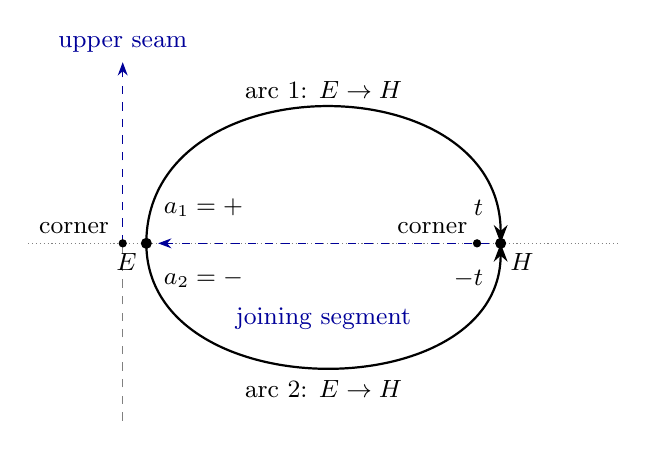
\begin{tikzpicture}[x=1cm,y=1cm,>=Stealth,font=\small]
 \draw[gray,densely dotted] (-.5,0)--(7,0);
 \draw[thick,->] (1,0) .. controls (1,2.3) and (5.5,2.3) .. (5.5,0);
 \draw[thick,->] (1,0) .. controls (1,-2.1) and (5.5,-2.1) .. (5.5,0);
 \draw[gray,dashed] (.7,-2.25)--(.7,0);
 \draw[blue!60!black,dashed,->] (.7,0)--(.7,2.3)
   node[above] {upper seam};
 \draw[blue!60!black,dashed,->] (5.35,0)--(1.15,0)
   node[midway,below=7mm] {joining segment};
 \fill (1,0) circle (2pt) node[below left] {$E$};
 \fill (5.5,0) circle (2pt) node[below right] {$H$};
 \fill (.7,0) circle (1.5pt);
 \fill (5.2,0) circle (1.5pt);
 \node[above left] at (.65,0) {corner};
 \node[above left] at (5.2,0) {corner};
 \node at (3.25,1.95) {arc 1: $E\to H$};
 \node at (3.25,-1.85) {arc 2: $E\to H$};
 \node[right] at (1.1,.45) {$a_1=+$};
 \node[right] at (1.1,-.45) {$a_2=-$};
 \node[left] at (5.4,.45) {$t$};
 \node[left] at (5.4,-.45) {$-t$};
\end{tikzpicture}
\caption{Cuts and orientations for the marked pairing, drawn schematically in the square-tile coordinates. The displayed contractible example has $t=-1$; the argument also permits essential polygons and arbitrary segment crossings. Both arcs are oriented from $E$ to $H$, so the actual polygon is arc 1 followed by the reverse of arc 2. Only the upper part of the seam changes twist, starting at the corner just before $E$; closing along the dashed horizontal segment defines the turn degrees $n_j$.}
\label{fig:marked-phase}
\end{figure}

For the simple actual polygon oriented by arc 1 followed by reverse arc 2, turn degree plus leftward winding is \(\epsilon=\pm1\), positive if its bounded or lower side lies on its left. Its turn and winding are \((W_1-W_2)/(2\pi)\) (in revolutions) and \(h_1-h_2\). Also \(X_1-X_2=-(1+t)/2\) by testing its left side just east of the first mark and just west of the second (indicators 0 and \((1+t)/2\), respectively, decreasing by one at upward crossings in moving eastward).

Hence \(D_j=n_j+h_j+X_j\) are odd with \(D_1-D_2=\epsilon-1\). Before switching the upper twist, the turn, seam and insertion phases have product
\[
 \exp\!\left(\frac{i(W_1+W_2)}4\right)
       i^{h_1+h_2}i^{X_1+X_2}=i^{D_1+D_2},
\]
since the endpoint corrections cancel in \(n_1+n_2\). This phase is \(-1\) exactly when \(\epsilon=1\). The switch of twist upstairs toggles sign exactly in that case: its crossing parity is odd precisely when the corner just west of \(E\) lies in the bounded or lower side. The resulting weight is therefore positive. The unique arc orientations identified at the start show that each polygon contributes once; height exhaustion proves the assertion.
\end{proof}

\subsection{A direct estimate when the marks are antipodal}\label{c6:subheading-16}

The homogeneous antipodal case gives a direct route from the physical
pairing to the correlation exponent using the two-line gas already
constructed.  It displays the quotient by the zero separating-loop
partition and derives the magnetic test potential, its scalar
normalization, and the contour estimates reused below.  We retain this
calculation for those identities and for its independent homogeneous
estimate, stated here at exponent-level precision.  The later argument
treats varying staircase rapidities and unequal intervals with uniform
constants: when $d\ll N$, two long intervals lie outside the short
magnetic core, and their open operator product requires control that
this homogeneous calculation does not provide.

On the homogeneous cylinder of even period with antipodal row sites, the polygon mass just identified satisfies
\[
 K_2 \le (m+1)^{-4/3+o(1)}\qquad\text{(period }2m+2\text{)} .
\]

\paragraph{Normalization and magnetic potential.}
We detail the changes in the two-line gas estimate (notation \(\eqref{eq:legacy-P-star}\) there). Start with all common labels \(+\). In the residue representation for \(k=2,l=h=1,n=m,\delta=i\), at homogeneous extra rapidities, the extra-slot factors supply \(J(v)^2\) at an unlowered common site of rapidity \(v\), then multiply by \(\cos^2 z/\cos^2(z+b)\) per lowering concentrated at \(z=v-L\) or \(v-2L\), by the \(M\)-table. They therefore just supply that latter factor as additional potential (one can still split the common poles keeping all extra variables at zero). Normalize off the all-positive coefficient product \(Q_{11} C^m D(0)^{m(m-1)}J(0)^{4m}\), calling the remaining residue sum \(P'_m\). Put \(M=m+1\). Since \(D(0)=J(0)^2\) and \(Q_{11}=C/2\), the two prefactors agree exactly:
\[
\begin{aligned}
 Y&=\frac{C^M D(0)^{M(M-1)}}2\,P'_m,\\
 f_{2M}(0)^2&=\frac{C^M D(0)^{M(M-1)}}2\,P_M(i).
\end{aligned}
\]
The second identity is the cylinder formula at zero separating-loop weight. Thus the physical mass is \(P'_m/P_M(i)\).

The elementary potential at \(z=iw\) is now \(e^{M V(w)} [-\sin(z+L)/\sin(z-L)]\). In the residue lift use the periodized first factor from the gas argument (with \(M\) replacing \(m\)), and replace the bracket by
\[
 U_T(w)=-\frac{S_T(w-iL)}{S_T(w+iL)}
   \left(e^{-3iL}\frac{S_T(w-T/2+iL)}{S_T(w-T/2+4iL)}\right)^2 .
\]
Indeed \(U_T\) is periodic with period \(T\), tends to the bracket and is analytic in \(e^{-T}\) near zero there in the sense of local germs at the finite contours. Its zero at \(w=iL\) also restores pole multiplicity \(m\). The lifted residue calculation is a finite grand sum analytic near the nome disk down to its center, by splitting poles as before (same zeros enforcing exclusion on center deposits). There is no new pole crossing in opening contours. On the right use \(a(w)=\log U_T(w)\), branch close at 0 to zero, analytic and periodic on the right strip reaching any width \(<L\) on either side (real large period for now). Indeed the first ratio's continuous log increases by \(12iL\) over a period, the edge ratios together compensate by \(-12iL\); equivalently use the coth differences for the logarithmic derivative or the defining products, continued along the real line. Write \(\bar a\) for its period mean, and use hats for the period integrals in the convention fixed at the start of Section~\ref{c6:gas}.

\paragraph{Transforming the magnetic test.}
Here are details of carrying this factor through the previous transform. First separate \(\exp\allowbreak(2K_{\rm count}\bar a)\): thus use \(r=-2\bar a\) in \(\eqref{eq:legacy-P-star}\), with external factor \(\exp(2M\bar a)\). On each original left elementary member retain \(e^{-\bar a}U_T\); on the right add \(a-\bar a\) to each color's Cartan test potential. Winding phases and zero-mode constraints are unchanged. Thus in addition to replacing \(m,r\) as indicated, and retaining the original-left factors and external factor, add to the exponent
\[
 \frac1T\sum_{p\ne0}
 \left[2M\widehat\rho(p)\widehat a(p)+Q_+(p)\widehat a(-p)\widehat a(p)
 -\sum_{d} e^{-ip s_d}\frac{2\pi}{p}e^{\delta_{i_d} x} A_{i_d}(z_*) Q_+(p)\widehat a(p)\right],
 \quad z_*=e^x,\ x=Lp ,
\]
where \(Q_+\) denotes the common-color eigenvalue of \(Q=K^{-1}\) in the mode calculation, and \(A_i\) likewise the common-color coupling functions there. Indeed this is exactly the nonzero-mode Cartan completion described above.

The analyticity for moving inverse currents and convergence for fixed left data are unchanged by the mean-zero test. The extra Schur linear term permits the prescribed subsequent contour moves as well (\(A_i\) are bounded on both high-frequency ends by the given rational functions, \(|\delta_i|\le1/2\) throughout, whereas the test has decay out to any width less than \(L\)). For the original-left multipliers one uses the larger meromorphic strip rather than the logarithm's strip. The nearest pole boundaries of \(U_T\), in imaginary-offset units, are
\[
 \begin{array}{c|c}
 \text{center}&\text{pole-free interval}\\\hline
 0&(-L,7L)\\
 T/2&(-4L,4L)
 \end{array}
\]
modulo the imaginary period \(8L=\pi\). The original elementary offsets used in the deformation lie between 0 and \(37L/12\), strictly inside both intervals. Thus no additional residues occur; on fusion the linear sources add. These arguments can first be made at fixed Fourier coefficient in the common fugacity and identified as in the justification of \(\eqref{eq:legacy-P-star}\), using absolute convergence (also on any full fugacity period, with weaker bulk bounds) as verified below.

Recall \(a_0=\pi/b=8/3\) and \(h_*=3\pi b/4=9\pi^2/32\). Use \(T'=\Re T=(2/a_0)\log M+g\), with large fixed \(g\), allowing bounded nearby perturbation in real part and \(|\Im T|<\pi+1\). We record estimates on the continued graph from the gas argument, taken antisymmetric and passing through \(\pm T/2\); as before it can be varied holomorphically about the real central period, with zero displacement in the indicated core. Constants can depend on \(g\). On this curve
\[
 a(w)=i\,6L\operatorname{sgn}(\Re w)
   + O(e^{-c|\Re w|}+e^{-c(T'/2-|\Re w|)}) ,
 \qquad \bar a=O(1/T')
\]
in the central interval. Indeed this follows from the defining products; the transition profiles remain bounded, also on small strip neighborhoods reached by displacements of any fixed width strictly below \(L\) when the curve stays close to 0 or the corresponding period edge (use the small Lipschitz slope relative to these centers). Direct original-left factors have bounded modulus too: their elementary offsets above the graph are between 0 and \(37L/12\), lying strictly inside the relevant pole boundaries \((-L,7L)\) at 0 and \((-4L,4L)\) at the period edge. Imaginary deviations near those centers are controlled relatively by the small slope.

The quadratic added scalar then equals
\[
 -\frac{(6L)^2}{h_*}\,T+O(1).
\]
To see this one may use the straight complex period just for the scalar. Integration by parts and small parallel displacements give \(|\widehat a(p)|\le C e^{-c|p|}/|p|\) off zero by localized derivative bounds. Replacing \(Q_+\) by \(1/h_*\) thus costs \(O(1)\), by even regularity at zero and at-most-polynomial high-frequency growth, and the remaining term integrates \((a-\bar a)^2/h_*\).

The cross scalar with \(M\) including \(2M\bar a\) is \(c_3 M e^{-T}+O(1)\) for a constant \(c_3\). Indeed it integrates \(2M a\) against the periodization of \(\rho\). The core ratio has odd log in the central interval, with the specified branch. The normalized squared edge ratio there has log with first term \(e^{-T}(d_1 e^{2w}+d_2 e^{-2w})\), with constant \(d_1,d_2\), and bounded error \(C e^{-2T'+4|\Re w|}\), directly expanding the products away from the edges, using boundedness near them. Keep just the unshifted density on this first term and extend the resulting integral to the whole real line by analyticity; image terms, tails and product errors after integration cost \(O(M e^{-a_0 T'/2})\), using \(2<a_0=8/3<4\) and the explicit density. Continued integrals have the same estimates.

Finally the added Schur per-particle term (the term with \(A_i\)) has real part
\[
 \frac{2\pi\cdot6L}{h_*}\,W_d |\Re s_d|+O(1).
\]
Indeed \(A_i(1)=-W_d\); retaining the pole \(2\pi W_d/(p h_*)\) gives this mean-zero primitive of \(-i(a-\bar a)\) times \(2\pi W_d/h_*\), up to an additive centering constant independent of particle except for the factor \(W_d\). Here and in this display such a constant is discarded by winding neutrality. The sign profile estimate proves the formula for that primitive. The remainder multiplier at zero is regular. Its constant value there applied to \(a-\bar a\) costs \(O(1)\). After subtracting that too, it acts boundedly throughout analytic transport.

For detail, \(a'\) is the periodization of two localized coth differences, translated by 0 and \(T/2\). Their whole-line transforms separately are regular at zero, decay with any exponential weight of rate \(<L\), and have the same bounds (measuring rate in \(|\Re p|\)) along tails of small sector slope; indeed integrate the coth differences across one vertical period \(i\pi\), obtaining finite sums of pole exponentials divided by \(1-e^{-\pi |p|}\) on each real ray before continuation. Thus after the pole and constant subtractions the products of these transforms with the remaining multiplier divided by \(-ip\) are regular near zero and decay exponentially on slightly bent, shifted Fourier contours (allowing also the factors with shifts \(\delta_i L\)). Their inverse transforms decay exponentially about each respective center along the small-slope complex graphs, by the same contour shift and tail bending used for the regular energy symbols. Ordinary periodization gives the asserted bounded continued remainder, with the ordinary zero mode removable (the two derivative masses sum to zero).

By neutrality the linear bias just estimated can be written, in real part and up to \(O(N_0)\), as
\(- (12\pi L/h_*)\sum_d W_d(T'/2-|\Re s_d|)\). Its unfavorable terms all have \(\sigma\ne0\); thus a fraction of the original suppression \(-c M e^{-a_0 |\Re s|}\) absorbs them at bounded cost per particle (fixed \(g\)). Since \(r=O(1/T')\), the coercivity, tilt and localization estimates \eqref{eq:legacy-P-P2},\eqref{eq:legacy-P-P3} and factorial summation now give total cost \(O(1)\) in log from particles and the Poisson sum, apart from the already retained scalars. For verifying convergence with an independent fugacity test on a full Fourier period one can as before lose \(O(T')\) to the bounded tilt. The same estimates justify analytic transport termwise on the small-slope graph as in the uninserted calculation.

\paragraph{The scalar bound and maximum modulus.}
The original bulk scalar with \(M\) has log real part
\[
 M^2 I+2 M^2\Re(A e^{-2T})+(3/8)\log M+O(1)
\]
by the scalar estimates for the gas (here \(M^2 e^{-a_0T'}=O(1)\), and the Riemann sum for the log determinant has bounded additive error by exponential decay and integrable derivative, also replacing \(T\) by \(T'\) there at bounded cost). Multiply the analytic residue sum by \(\exp(-2 A M^2 e^{-2T}-c_3 M e^{-T})\) and apply maximum modulus in the nome \(e^{-T}\); the multiplier is 1 at the desired center. We conclude
\[
 \log|P'_m|\le M^2 I+\left(\tfrac38-\tfrac32\right)\log M+O(1),
\]
since \((6L)^2(2/a_0)/h_*=3/2\). Equation~\eqref{eq:gas-individual-saturation} gives
\(\log P_M(i)\ge M^2I+(5/24+o(1))\log M\). Dividing the two estimates leaves
\[
 \left(\frac38-\frac32\right)-\frac5{24}=-\frac43,
\]
which proves the stated exponent-level bound.

\subsection{Staircases and the two background lists}\label{c6:unequal-marks}



We now prove Theorem~\ref{u:two-edge-theorem}.  Keep its notation $P,d,k,N$ and the two marked edges.  The insertion identity \eqref{eq:finite-marked-contraction} is unchanged, but its two lists now have different lengths.  The proof must keep the resulting two scales separate: a core of logarithmic length proportional to $\log d$, and the whole period of length proportional to $\log N$.  All constants below are independent of $P_1,P_2$ and $k$.



\begin{figure}[htbp]
\centering
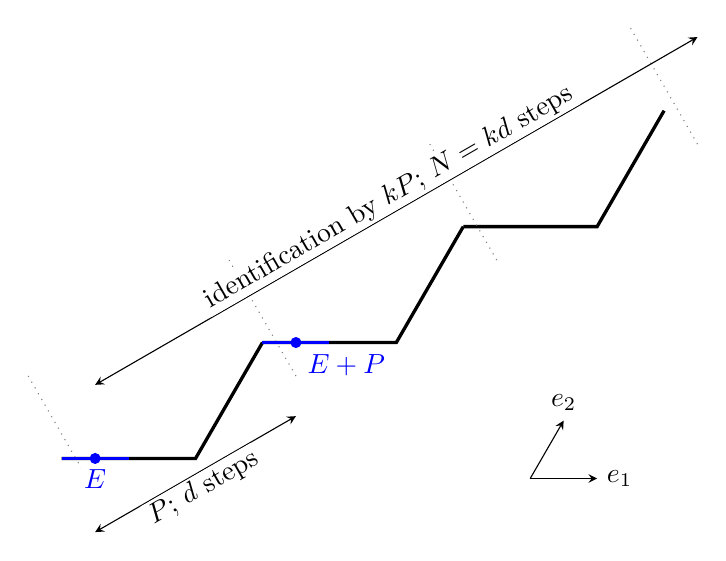
\begin{tikzpicture}[x=0.85cm,y=0.85cm,>=stealth]
  \foreach \j in {0,1,2} {
    \draw[very thick] ({3*\j},{1.73205*\j})
      -- ({3*\j+2},{1.73205*\j})
      -- ({3*\j+3},{1.73205*\j+1.73205});
    \draw[gray,dotted] ({3*\j+0.5},{1.73205*\j-0.5})
      -- ({3*\j-0.5},{1.73205*\j+1.23205});
  }
  \draw[gray,dotted] (9.5,4.69615)--(8.5,6.42820);
  \draw[very thick,blue] (0,0)--(1,0);
  \draw[very thick,blue] (3,1.73205)--(4,1.73205);
  \fill[blue] (0.5,0) circle (2pt) node[below=3pt,fill=white,inner sep=1pt] {$E$};
  \fill[blue] (3.5,1.73205) circle (2pt) node[below right=3pt,fill=white,inner sep=1pt] {$E+P$};
  \draw[<->] (0.5,-1.1)--(3.5,0.63205)
      node[midway,below,sloped,fill=white,inner sep=1pt] {$P$; $d$ steps};
  \draw[<->] (0.5,1.1)--(9.5,6.29615)
      node[midway,above,sloped,fill=white,inner sep=1pt] {identification by $kP$; $N=kd$ steps};
  \draw[->] (7,-0.3)--(8,-0.3) node[right] {$e_1$};
  \draw[->] (7,-0.3)--(7.5,0.56603) node[above] {$e_2$};
\end{tikzpicture}
\caption{A monotone staircase carrying the two identical translated marks.
The example has $P_1=P_2=2$ and $k=3$.  Translating the staircase in the
third edge direction produces the lozenge rows; the dotted segments
indicate that transverse direction.  The two background lists have
lengths $d$ and $N-d$ after adjoining one marked site to each.}
\label{u:staircase-figure}
\end{figure}


Use a row cut obtained by a periodic monotone staircase in \(e_1,e_2\) (period \(P\), passing through the marks), and translate it in the third lattice-edge direction to make rows. This tiles by lozenges with acute or obtuse angle at the corner between the increasing row and the transverse vector; drawing as square tiles, the same honeycomb path weights are given by \(R(t+v_i)\) at argument \(L\) or \(2L\), respectively (the two choices reflect the base angle, interchanging \(a,h\) and \(c,d\) in the tile notation). By lattice reflection if necessary take the majority steps to have argument \(2L\). The infinite-height projection and orientation argument for the two marks in the flip formula therefore apply verbatim to these physical column parameters (above, their negatives in the formula by crossing). For the use of the projection, lifted individual arches have summable mass and through-lines to height tending to infinity have vanishing mass at fixed \(N\). Indeed in the planar lifted slab or half-plane bounded by these stairs the contour from a fixed boundary source has a common rotated real coefficient bounded positively: turns to other boundary exits are given by cyclic outward-normal differences minus \(\pi\), with a single consecutive pair of lattice normals for the rounding, so only one sign of excess up to \(\pi/3\) is possible. Transversal pure cuts can truncate the sides. For decay cut further by a pure hexagon of radius comparable to height. Mass to the hexagon cuts is \(O_N(r^{-1/4})\): average over order \(r/N\) translations by whole periods putting the starts at distinct positions in the central part of a common smaller hexagon (contour subtraction before translating), and reverse at the pure sides to use their escape bound in a positive contour, with order \(r\) such exits. This is the flat-side argument of the geometric estimates. Thus through-line systems disappear by absolute single-path bounds and empty projections have the same limits.



For detail use lattice coordinates \((X,Y)\) along \(e_1,e_2\), with transverse step \(e_2-e_1\). Between transverse truncations (bounds on \(X+Y\)) and the two periodic stairs this domain has lower and upper bounds on \(Y\) as functions of \(X+Y\), both with slopes 0 or 1. Intersecting with pure hexagons or parallel pure half-planes (bounds on \(X,Y,X+Y\) at lattice levels) retains that same form: the bounds use maxima/minima, with feasible section on an interval since comparison with each affine bound uses monotonicity (of both stair coordinates). The CCW tangent directions thus occur in a lower block alternating directions 0,1, then possibly direction 2, upper block using 3,4, possibly direction 5 (units \(\pi/3\)). The cyclic tangent increase to exits from a given boundary midpoint therefore stays in either \([-\pi/3,2\pi]\) or \([0,2\pi+\pi/3]\), depending on the starting direction. Subtract \(\pi\) to get the path turn by boundary closure. This gives the asserted rotated positivity since \((3/8)(2\pi+\pi/3)<\pi\), and applies to subtraction of signed contours as before (terms on shared exits which stay inside agree). The planar flux rule still applies in these simply connected regions. To bound through mass from one stair in a wide truncation at fixed period, take a common lattice hexagon centered near that start of radius comparable to slab height but small enough not to reach the opposite stair. Start also at its period translates in the central part, and subtract the contour in the intersection to bound the individual through masses by the mass to the hexagon cuts. Upon reversal from each such new exit, cut again parallel to its pure side before the central targets; subtraction bounds their mass by that to the new line, at most a constant times the straight strip bridge sum at comparable scale. Letting the transverse truncations recede, the through masses are equal by periodicity. This gives the bound stated above. Arch sums themselves are bounded just by the positive contour, using exhaustion.



Both extra rapidities in each column now have the same value, denoted \(x_e\). The two common lists have sizes \(m=d-1,n=N-d-1\). Augment each for the plasma calculation by one site at \(x_e\), forming background lists of sizes \(M_A=d,M_B=N-d\), both even, now having identical proportions of the two possible values. In this section use \(\lambda_b=\pi/(2b)\); write \(\lambda\) for the proportion of minority steps, \(0<\lambda\le1/2\). By translation of rapidities we take the majority value to be \(r_0 L\) and the minority \((r_0-1)L\), where \(r_0=1/4+\lambda/2\).



The residue calculation starts from all common labels positive (whether neutral then or not), using its product as prefactor. Exactly as in the balanced two-leg case the potentials are now one copy of \(R_{g h}(i(w+i v_e))\) per augmented-list site \(e\) of color \(h\), value \(v_e\), and the common magnetic factor \(-\sinh(w+i x_e-iL)/\sinh(w+i x_e+iL)\); this follows by translation in each extra-slot factor of that calculation. Denote the remaining residue sum by \(P'\). The prefactor divided by \(f_N^2\) in the observable is
\begin{equation}
 \frac{C^{N/2}\prod_{e<f:\ g_e=g_f}D(v_e-v_f)}{2 f_N^2}
 \prod_{e\text{ common}} \frac{J(v_e-x_e)}{J(x_e-v_e)}
 \label{eq:legacy-P-23}
\end{equation}
by \(D(y)=J(y)J(-y)\), \(Q_{11}=C/2\). Elementary lowering counts satisfy \(K_g=M_g+u\) with common integer \(u\).



Periodize as before, using magnetic factor
\[
 U_T(w)=-\frac{S_T(w+i x_e-iL)}{S_T(w+i x_e+iL)}
 \left(e^{-3iL}\frac{S_T(w-T/2+iL)}{S_T(w-T/2+4iL)}\right)^2,
\]
and in the central theta sum include background charges \(q_e=-q_{g_e}\) at offsets \(a_e=-v_e\) (to avoid confusion, \(q_{g_e}\) itself denotes the color sign as for a particle). Thus \(X\) in the center Gaussian includes \(\sum_e q_e i a_e\). This ensures periodic differentials. Initially use rapidities near zero, so all contour openings and deformations work by continuation. The lift is still a finite sum analytic near nome zero, by split poles as before. At final rapidities differences \(L\) in the site lists one uses limits: before opening, the individual residue terms obtained by splitting have only denominators from the displayed shifted \(S_T\)'s and constants, independent of counts of sites except via multiplicities. Possible singularities at exact differences stay on the very same pair hyperplanes independently of nome on the small disk. Removability there for the lifted sum will also follow below by analytic continuation in rapidities of the final integral bounds (identity first for real periods). Thus maximum modulus at those values is permitted.



\subsection{The ordered magnetic gas}
\label{u:ordered-gas}

The staircase determines the background lists.  We next express their
residue sum as an ordered gas whose integer height records the winding.
Keeping the phases in this step is essential: the interval estimate below
uses the resulting transfer operator, not the absolute value of an
unidentified periodic partition function.

Here are details of extending the mode calculation. Put \(E(p)=\sum_e e^{-p a_e}{\bf e}_{g_e}\). In the mode matrix include extra background slots \(E_e\) with count-mode 1, pair entries from the potential factors (so \({\cal M}_{R,E}n_E=-K\widehat\rho E\)), inverse couplings to them initially zero. Their mutual block is zero except that formally at Laurent zero assign the pole terms
\(4q_eq_f/p^2+4q_e q_f(a_e-a_f)/p\), of zero finite part. Then:


\begin{itemize}

\item 

The bulk term in log is
\begin{equation}
 S(T)=\frac1{2T}\sum_p E(-p)^t K(p) E(p)\widehat\rho(p)^2
 -\frac12(T/3-2\log2)(M_A-M_B)^2.
 \label{eq:legacy-P-24}
\end{equation}
Determinants and measure conventions in \(\eqref{eq:legacy-P-star}\) are unchanged.



\item 

Chemical potentials per final particle (before adding the magnetic test) are
\begin{equation}
 2\pi i\,\sigma_i\sum_{e:g_e=g_i}
 \int_0^{s+i(v_e+\delta_i L)}\sum_{\nu\in\mathbb Z}\rho(z+\nu T)\,dz ,
 \qquad \sigma=(0,1,1,-1,0).
 \label{eq:legacy-P-25}
\end{equation}
Fugacity \(e^{-u r}\) if used still brings \(T r_j^2/(4h_*)-r_j(u_*+\bar L)\).
Indeed distribute \(2X^2\) into all pairs including background-background. The terms with \((a_i-a_j)^2\) in units of \(1/T\) again sum to \(-2 A_{\rm tot}^2\) with all charged offsets included; the missing constant logs from the background block give just the second term of \eqref{eq:legacy-P-24}. Thus the same verification by \(\gamma\) and its two charge conditions works with the extended block, including the center terms with \(l\); the Laurent saddle adds \(\widehat\rho E\) to the earlier residual saddle, giving the same common-integer Poisson sum and \eqref{eq:legacy-P-24}. In the chemical calculation the old simplifications apply in both color sectors individually: with \(H_V\) defined like \(H\) using multipliers \((0,-1,0,0,2c,0,0,-1)\), one has \((H_V+H\widehat\rho)(a;t)\) at \((0;0),(2;1),(2;-1),(3;-1)\) respectively \(0,0,\widehat\rho,0\). Insert the rapidity shift exponent to obtain \eqref{eq:legacy-P-25}. These formulas are for analytic continuation, so \(\sigma=0\) terms stay absent even beyond a primitive strip.



\end{itemize}


More explicitly at zero take the raw right count vector with left and inverse modes as before, appending background modes identically 1, and prescribe the same derivative condition \(q^t\gamma'_{\rm raw}=A_L+\sum_e q_e a_e+\pi l/2\). Then the second-order and first-order poles of the extended matrix still have the displayed charge/offset/winding form of the gas proof, so evaluation gives the actual center Gaussian and winding phases (including phase slopes from the potentials on left contours). The sum of charge products for pairs including real charges but not background-background alone is \(-\tfrac12(M_A-M_B)^2\) minus half the elementary count; regular diagonals treat the latter part as before. The additional saddle term \(\widehat\rho E\) neutralizes the appended charges at 0 and contributes exactly \(\sum_e q_e a_e\) to the derivative charge sum, while its count value \((M_A,M_B)\) leaves the free integer and Gaussian shift unchanged. The assigned background block has zero contracted finite part of its own. For \eqref{eq:legacy-P-25} the remaining linear symbol at a particle against each same-color site is \(-2\pi\sigma_i e^{(v_e+\delta_i L)p}\widehat\rho(p)/p\), yielding that primitive including the finite part at zero.



We describe the ordered-position form of the residual sum. Let \(\ell_{gi}\) count original left elementary members of species-color index \(i\) belonging to \(g\), write \(\ell_{\Sigma i}=\sum_g\ell_{gi}\). For particles in increasing order of real contours, write \(H(s)=j+\sum_{\Re s_d>\Re s} W_d\), \(j\) the Poisson integer; at a jump use its mid-value \(H_m\). Winding neutrality closes this integer path. Set the real row \(c^t\) by
\[
 {\bf1}^t(J(p)-K(p)\ell)=2\pi W^t/p-2h_* c^t+O(p).
\]
(In this expression \(J\) is the coupling block of the transform, transported on the final constituents, not the site function in \eqref{eq:legacy-P-23}.) Thus \(u_*+\bar L=c^t n-(\pi i/h_*)\sum W_d s_d\). At zero,
\begin{equation}
 Z=\alpha WW^t/p^2+M_*/p+O(1),\qquad
 M_*=-2\pi(\widetilde{\cal W}+W c^t-c W^t),
 \label{eq:legacy-P-26}
\end{equation}
where \(\widetilde{\cal W}\) is an integral skew matrix. Indeed change right variables by \(-\ell n\) in the block matrix before Schur. The non-right charges are now zero, its non-right block has simple coefficient \(-2\pi\widetilde{\cal W}\) from the shifted winding matrix (\({\cal W}_{nn}-\ell^t{\cal W}_{Rn}-{\cal W}_{nR}\ell\) before subsequent branch corrections). The remaining poles after Schur come just from the common channel as shown. Exact-offset averages for free left clusters give integral windings here (symmetric shifts for same offset clusters; otherwise all off singular offsets, even sum of multiplicities).



Apart from the explicit terms of \(\eqref{eq:legacy-P-star}\) and site/test couplings the constant phases, when \emph{combined} with the ordered factor from \(M_*/p\) and the term \(-2\pi i j c^t n\), reduce up to a single unit prefactor to
\begin{equation}
 \prod_d \eta_{i_d} \exp[-2\pi i c_{i_d} H_m(s_d)]
 \label{eq:legacy-P-27}
\end{equation}
for fixed unit constants per species, the same for every choice of even \(M_A,M_B\), including 0. Here and below indices in such products include the color. To check this, the \(1/p\) kernel at ordered separation is \(-i/2\) (positive separation), so neutrality gives the stated mid-value term and an unordered sign \((-1)^{\widetilde{\cal W}_{ab}}\) per pair. Before branch moves, original log constants have signs \((-1)^{{\cal W}_{ab}}\) on pairs of left particles, plus \((-1)^{\sum k_g P_g}\) from right-left pairs, where \(k_g=M_g+u-\sum_i\ell_{gi} n_i\) and \(P_g=({\cal W}_{R,L'} n_{L'})_g\); backgrounds contribute no sign (zero right winding, integral left windings and even counts near zero rapidities). Indeed for each shifted product of sinhs the positive-separation leading logs have just the offsets times \(i\), without extra signs before taking the indicated means and jump, since the products use symmetric shifts. Residue orientations can add single-cluster phases only. Original right and inverse same-side symmetrization gives exponents \(\sum_g\binom{k_g}2+\sum_{g,t}\binom{n_{gt}}2\), and the Weyl exponent adds \(\sum_g\lfloor(1-k_g-n_{I,g})/2\rfloor\), with \(n_{gt}\) inverse counts, \(n_{I,g}=\sum_t n_{gt}\). These are exactly the constant-mode signs in the trace calculation of \(\eqref{eq:legacy-P-star}\) (between different ordered oscillator radii the geometric log has zero constant phase). Dependence on \(u\) cancels since each simultaneous unit increment flips \(\sum_g(P_g+n_{I,g})=0\bmod2\). At \(u=0\) changing \(M_g\) by 2 also has no effect. Now on count space all second differences of this total sign exponent, mod 2, are precisely \(\widetilde{\cal W}\): in addition to the left-left and right-left terms, the binomials and floors (using \(\lfloor(1-h)/2\rfloor=\binom h2\bmod 2\) for integral \(h\)) contribute per group the polarization entries of shift type
\(\ell_g\otimes n_{I,g}+n_{I,g}\otimes\ell_g+n_{g+}\otimes n_{g-}+n_{g-}\otimes n_{g+}\) (symbols here denote linear count functions). These give the inverse-inverse and shifted right-inverse windings. This cancels the unordered signs from \eqref{eq:legacy-P-26}, leaving just single-particle phases. Each subsequent branch change of order \(\nu\) shifts \(\widetilde{\cal W}\) correspondingly and brings the matching constant sign \((-1)^\nu\) between the pair by the ratio of geometric factors as in the mode calculation. Fusion restricts to sums of constituents (self-residue has only a local extra phase), with the same compensation for exterior pair branch changes. This proves \eqref{eq:legacy-P-27}.



For the short part of pair energy we use the periodization of \(G_{ab}(s)\) for ordered positive separations (target to the right, source to the left), with the usual regular diagonal at contact and both periodic continuations counted, once per positively separated pair up to translations. This denotes the inverse Fourier kernel after removing exactly the two pole kernels in \eqref{eq:legacy-P-26}, with transpose at negative separations. Thus the off-contact exponent in the gas is minus one copy of \(G\) per such pair, including pairs with translated particles, and the regular contact self term with half weight. For \(\Re s>0\) we have
\begin{equation}
 G_{ab}(s)=\sum_{l\ge1}\sum_{k=0}^{r_*} C_{ab,l,k}s^k e^{-\omega_l s},
 \label{eq:legacy-P-28}
\end{equation}
where \(\omega_l>0\) increase at least linearly, \(C\) grow at most polynomially and \(r_*\) is fixed. Indeed the rational functions in the final symbols of the two-line calculation have only unit-circle poles in \(e^{Lp}\), of uniformly bounded order (the extra denominators after Schur come from \(H_*\), proportional in the channel symbol to \((1-e)(\coth(bp)-c\,{\rm csch}(bp))\), and use the earlier factorization of \(1-e\)). Shifting the inverse contour downwards in imaginary-period multiples picks these residues apart from the already separated zero pole terms. The horizontal ends can be bent down at small slope (symbols subtracted at zero are bounded or \(O(1/p)\) there); equivalently for the unsubtracted meromorphic symbol use a principal finite-part integral, whose zero pole contributes just the two displayed long kernels. Along deep level shifts chosen a fixed distance from poles the tail rotation yields exponentially vanishing remainder. This agrees at real periods with the ordinary periodized short kernel by Fourier inversion (at contact the one-sided short parts can have a jump; for the self entry there is no jump), and then by the continuation of \(\eqref{eq:legacy-P-star}\). More explicitly removing \(\alpha WW^t/p^2+M_*/p\) gives a symbol regular at zero, \(O(1/|p|)\) at either end, with inverse integrable at zero (log plus bounded terms). Its ordinary periodization includes the exact zero harmonic; the pole kernels separately are as in \eqref{eq:legacy-P-P3}.



\subsection{From periodic gas estimates to interval operators}
\label{u:interval-operator}

We next construct an operator whose products describe intervals of the
ordered gas.  This construction is needed because the magnetic core and
the two exterior intervals have different particle potentials.  A bound
on homogeneous closed periods would not by itself control their product.

Here is the required transfer estimate. Fix a large cell length \(S_0\); consider first a homogeneous gas with no magnetic functions or \eqref{eq:legacy-P-25}, but take \(r=-2a_0'\) constant, \(a_0'=+6Li\) or \(-6Li\), and allow all five species of color \(A\), only \(S,F\) of color \(B\). In addition to \(G\) and \eqref{eq:legacy-P-27} this has exponent
\begin{equation}
 -h_*^{-1}\int(\pi H+i a_0')^2\,ds
 + 2a_0' c^t n.
 \label{eq:legacy-P-29}
\end{equation}
The construction below will give a common state space for the two tilts; Lemma~\ref{lem:u-homogeneous-operator} then states the strict spectral bound.



\paragraph{Coercive gauge and nearest cells.}
We specify the operator since a pressure comparison on closed periods, without controlling intervals, would not suffice. A cell state \(x\) consists of the incoming integer height and indistinguishable points of each species/color in an open interval of length \(S_0\), with their factorial Lebesgue measure using the particle normalization of \(\eqref{eq:legacy-P-star}\). Include all species of both colors in the ambient space even if some are suppressed by zero point weights. Along an edge \(x\to y\) require outgoing height of \(x\) equals incoming of \(y\).

Use the real reference energy at zero tilt, no extra particle potentials: \(A(x,y)\) is half each of the two cell self energies (including \(\pi^2/h_*\int H^2\)), plus the real adjacent pair energy from \eqref{eq:legacy-P-28}. Cyclic sums omit just separations of at least two cells in \eqref{eq:legacy-P-28}. By \eqref{eq:legacy-P-P3}, for large fixed \(S_0\) they satisfy
\begin{equation}
 \sum A(x_i,x_{i+1})\ge 4\epsilon_S\sum_i |x_i|_0^2-C_S n_{\rm cells},
 \qquad |x|_0^2=N_x^2+H_{x,\rm in}^2 ,
 \label{eq:legacy-P-30}
\end{equation}
where \(N_x\) is total particle count, \(\epsilon_S>0\) at least inverse-polynomially small in \(S_0\). Indeed omitted terms cost exponentially small times \(\sum N_x^2\); interval counts in \eqref{eq:legacy-P-P3} control \(\sum N_x^2/(1+S_0)\), and incoming height is controlled by within-cell heights and counts. Here \eqref{eq:legacy-P-P3} at real large period is independent of the number of site sources; its proof holds for every large period. One may repeat a short cycle before applying it. Coincident points inside cells need not be used.



There is then a finite Borel real function \(\phi(x)\) on these states away from coincidences such that
\[
 A(x,y)\ge 2\epsilon_S(|x|_0^2+|y|_0^2)-C_S+\phi(y)-\phi(x).
\]
Indeed take the infimum of corrected path sums (subtract the count squares, add \(C_S\)) from an empty cell of height zero. There are finite paths both from the empty state to any prescribed
state and back, because jumps of both unit signs are available.  A fixed
return path and \eqref{eq:legacy-P-30} bound all corrected forward path costs from below;
a fixed forward path bounds their infimum from above.  The infimum is
therefore finite.  On each component with prescribed particle counts
and height, the energy is continuous away from coincidences.  Taking
intermediate positions in fixed countable dense subsets consequently
leaves the infimum unchanged and makes it a Borel function of the terminal state.

Gauge every forward transfer edge by \(\exp(\phi(y)-\phi(x))\). The gauge cancels on cycles. Complex nearest-cell weights use the same split into halves on self terms including the real reference height square, and all adjacent interactions as above; other point, height and oriented phase terms can be assigned wholly to the first cell on its outgoing edge. The gauge provides Gaussian margins in both endpoint states.

It still does so for small-slope complex deformations of the cells (holomorphic off null sets). Specifically compare curves parametrized over the same real intervals with derivative within a sufficiently small constant of 1 and with differences of successive position shifts Lipschitz-small, including across ends. The derivative of the short kernel away from 0 on that sector is bounded by \(C(1+1/|\Re s|)e^{-\gamma|\Re s|}\) by contour rotation as in \eqref{eq:legacy-P-P3}; self regular diagonal does not move. Thus local short comparison costs \(O_S(\text{slope error})(N_x^2+N_y^2)\). The height square has the same type of bound with also incoming heights; Jacobians can go into point weights.



\paragraph{Fock encoding of longer interactions.}
Encoding decaying pair interactions in a bosonic transfer space and recovering
periodic partitions from determinant-corrected traces has precedents in
one-dimensional spin systems~\cite[Sections~4--6]{HilgertRilke2008}.
Here the preceding gauge supplies the bounds needed for the unbounded
particle counts and integer heights.

For interactions of range at least two cells add a boson symmetric Fock space over countably many finite propagation blocks. They use semigroups \(D_d\) with each block generated by \(-\omega_l+\text{nilpotent}\), the nilpotent a bounded Jordan shift. Choose finitely many blocks per \(l\) and creation/detection arrays \(u_a,v_b\), with bilinear pairing in each block, so that
\[
 v_b D_d u_a=-G_{ba}(d)
\]
term by term in \eqref{eq:legacy-P-28}. The entries of these arrays need grow only polynomially in \(l\) before a rescaling; the unpropagated arrays need not be Hilbert-space vectors. Only the propagated sums below enter the Fock operators, and their square-summability will follow from the exponential decay. At edge \(x_i\to x_{i+1}\) the Fock state is passed from their common boundary to the next one; annihilate against \(V=\sum_{b\in x_{i+1}} v_b D_{d_b^L}\), where \(d_b^L\) is displacement within that cell from its left boundary. Propagate by \(D_{\ell'}\), \(\ell'\) the length (complex displacement) of \(x_{i+1}\); then create \(U=\sum_{a\in x_i}D_{\ell'+d_a^R}u_a\), \(d_a^R\) displacement from particle to right edge in \(x_i\). More precisely the Fock operator in forward order is
\[
 \exp a^\dagger(U)\ \Gamma(D_{\ell'})\ \exp a(V),
\]
with creation and annihilation in exponential-vector normalization, \([a(V),a^\dagger(U)]=VU\), and \(\Gamma\) symmetric tensor powers including vacuum.

By the rescaling \(u_a\mapsto e^{\omega_l S_0/3} u_a,\ v_b\mapsto e^{-\omega_l S_0/3}v_b\) modewise, \(\|U\|+\|V\|\le Ce^{-\epsilon S_0}(N_x+N_y)\). This Fock operator has trace norm at most \(C\exp(C\|U\|^2+C\|V\|^2)\). Indeed one can split \(\Gamma(D_{\ell'})=\Gamma(\tfrac12 I)\Gamma(4D_{\ell'})\Gamma(\tfrac12 I)\), with middle trace norm bounded by the convergent boson product of singular-value factors by strict summable contraction. Creation exponential times \(\Gamma(\tfrac12 I)\) is bounded as stated by its series (the \(k\)th power on degree \(m\) has norm at most \(\|U\|^k\sqrt{(m+k)!/m!}\)); likewise adjoint. Thus this cost is allowed within the Gaussian margins.

The resulting integral operators including the classical state on \(L^2\) are Hilbert-Schmidt. This remains true uniformly with bounded-above point log moduli per particle and bounded linear and constant perturbations of the volume height energies.



\begin{lemma}[Homogeneous interval operators]\label{lem:u-homogeneous-operator}
Choose $S_0$ sufficiently large and keep it fixed.  On the common
ambient cell space with Fock fibers constructed above, let
$\mathcal T_\pm$ be the homogeneous cell operators with all five species
of color $A$ and only $S,F$ of color $B$, the other species having zero
outgoing point weight.  There are no magnetic functions or potentials
\eqref{eq:legacy-P-25}; the constant tilt is $a_0'=\pm6Li$, $r=-2a_0'$,
and the weights consist of $G$, the phases \eqref{eq:legacy-P-27}, and
the exponent \eqref{eq:legacy-P-29}.  Then $\mathcal T_\pm$ are
Hilbert--Schmidt and their spectral radii satisfy
\[
 \operatorname{spr}(\mathcal T_\pm)<\exp(S_0/2).
\]
\end{lemma}
\begin{proof}
The construction proves the Hilbert--Schmidt assertion.  We prove the
spectral bound by identifying the cyclic traces and comparing two
representations of the same residue sum.

\paragraph{Cyclic traces and spectrum.}
Their ordinary traces of cyclic products (at least two edges) give exactly the ordered periodic gas times \(\det(I-D_T)^{-1}\), with \(T\) the whole period, this scalar tending to 1 at large period. In fact tracing the Fock product gives, besides this determinant, all contractions from previously propagated creations (also on earlier translates) into detections, hence sums precisely \eqref{eq:legacy-P-28} at positive separations of two or more cells, no others.

This identity follows simply by commuting exponentials, or Taylor-expanding on the occupation basis in finite blocks with the convergent geometric trace. In detail after multiplying into normal form \(e^{a^\dagger(P)}\Gamma(D_T)e^{a(B)}\) times its internal contractions, the normalized trace is \(\exp(B(I-D_T)^{-1}P)\). This follows by summing on each oscillator for diagonal \(D_T\), then for general strict contractions in finite dimension by conjugation on tensor powers and continuity; mode cutoffs converge by the bounds above. Internal and cyclic contractions then have the indicated time order.

The classical kernel trace formula with Fock fibers follows by Hilbert-Schmidt approximation, or composition and the Hilbert-Schmidt pairing (absolute kernel bounds Gaussian). For a homogeneous restriction suppressing species only by a point factor on outgoing sites the nonzero spectrum agrees with the restriction to allowed cell states, by block triangularity.



It suffices to bound homogeneous logarithmic trace per unit length on periods \(T=m_0S_0\), \(m_0\to\infty\). Indeed for a compact Hilbert-Schmidt operator the limsup root of absolute traces of powers is the spectral radius. For positive spectral radius one can split off by spectral projection the finite-dimensional outer eigenvalues with algebraic multiplicities; on the complementary invariant space smaller radius bounds even the power traces since two initial powers provide trace class. Leading eigenvalue powers cannot cancel at exponential scale along all integers (take simultaneous subsequences of phases tending to 1). We use here just the usual compact-operator spectral and spectral-radius facts (nonzero spectrum isolated poles of finite rank, \(\lim\|A^n\|^{1/n}\) equals spectral radius).



To bound those closed periods first fix real \(T\) large, and apply the two-line residue transform with \emph{no} magnetic potential, \(r=-2a_0'\), to backgrounds \(M_A=0,\ M_B\to\infty\) even with all variables zero. The original sum has no \(A\) particles because their original small residue contours have no site poles, and in particular only \(u=0\). Nevertheless opening and transforming both lines is still valid (coefficientwise proof as for \(\eqref{eq:legacy-P-star}\)). After removing \eqref{eq:legacy-P-24} the limit of the transformed gas keeps exactly the permitted species above, since nonzero \eqref{eq:legacy-P-25} on \(B\) have real part strictly negative proportional to \(M_B\) uniformly around this fixed real period. Dominated convergence follows from \eqref{eq:legacy-P-P3}. By \eqref{eq:legacy-P-26},\eqref{eq:legacy-P-27} and Coulomb integration the remaining exponent indeed has \eqref{eq:legacy-P-29}, since \(\int (H-j)=\sum W_d s_d\). Its determinant scalar per unit length in log is \(1/2+o(1)\).



\paragraph{The one-line comparison.}
The very same residue sum (without opening \(A\)) admits the one-right-line version of the current calculation on \(B\). Here are verification details. Use the heat period \(2bc_*\) with just one insertion in the normalized oscillator trace, \(K_{0,BB}=(2\pi/p)\coth(bp)\) and dressing factor \(1-e\) as before. A single Weyl reflection twists oscillator trace by oscillator sign, contributing the additional scalar \(\prod_{p>0}(1-e^{-2bp})/(1+e^{-2bp})\) and replacing Cartan covariance by \((p/2\pi)\tanh(bp)=K_{0,BB}^{-1}\). Indeed contractions run around with negative multiplier each time; the two inverse sides with the Cartan exponential then have evaluation multipliers \(-t e^{a_t p}\tanh(bp)\) including their own \(e^{-\phi}\), and the ordered inverse kernel uses this same \(\tanh(bp)\) in place of the reciprocal-channel multiplier, keeping the order subtraction in \(B(p)\). Equivalently these follow in \eqref{eq:legacy-P-P1} by moving the reflection to the end and replacing the oscillator occupation ratio in the one-line Wick contraction by \(-e^{-2bp}\) for \(p>0\). Gaussian integration again changes the reciprocal to that of \(K_{BB}\).

Zero momentum matching fixes \(q_B l=P_B+\sum t n_t\), allowing every choice of residual counts; the Laurent Schur saddle satisfies both charge conditions and no remaining mean Gaussian occurs (\(k_B=M_B-L_B\) fixed, \(Q\) vanishes quadratically at zero). Thus scalar \eqref{eq:legacy-P-24} is exactly the same; \eqref{eq:legacy-P-25} applies, and pair symbols through final fusion are precisely the given formulas with color entry \(c=0\), directly restricting original interactions to same color before Schur. Other zero factors have only polynomial growth in \(T\). All constant phase ambiguities here have unit modulus.



In slightly more detail, after moving the single reflection past the right inverse insertion the Cartan source has sign \(q_B\); relative to this sign the outer and inner inverse sources have signs \(-1,1\). Along the twisted oscillator trace the Cartan symmetric self contraction at harmonic \(\nu>0\) is \(\nu(1-h)/(1+h)\), \(h=e^{-2bc_*\nu}\), and ordered contractions use \(2\nu/(1+h)\), \(-2\nu h/(1+h)\); the momentum calculation at the insertion itself is unchanged. Thus even the inverse self terms have the same regular-diagonal convention (ordering singularity unchanged). Before the Schur step the Laurent pole matrices with winding are just restrictions of the earlier ones; the \(BB\) density block has leading \(4/p^2\), so its scalar equation at orders \(p^{-2},p^{-1}\) exactly enforces the count and derivative conditions against charge, leaving no order-zero quadratic correction. The twist product comes solely from the oscillator vacuum partition factor. No positivity of the twisted trace is being used.



For the analytic trace justification the preliminary inverse quadratic test from the two-line proof now has \(\Lambda=\tanh(bp)\), between the two tested values (the inequality is affine); all fixed-left convergence and subsequent termwise contour deformations therefore apply as there. The final same-color symmetric kernel is strictly positive with lower symbol bound \(\epsilon/(1+|p|)\), bounded real part at zero and high asymptotic \(2\pi I/|p|\).

We include the coefficient verification of positivity, since the one-line estimate is needed to control the operator on intervals. Take \(D_0(z)=(z^2-z+1)(z^4-z^2+1)\), \(t=e^{x/12}\), and \(H_{ij}=t^{-36+12(\delta_i-\delta_j)}D_0(t^{12})F_{ij}^{(0)}(t^{12})\), using \(x=Lp>0\). Clearing by positive scalars we want positivity of \((H+H^t)/(4\sinh x)\). Here \((H+H^t)/2\) is Laurent of degree at most 36 with coefficients at opposite powers negatives of one another (by substitution in the mode rules above). Let \(B_j\) denote its coefficient of \(t^j\), \(1\le j\le36\). Thus the matrix being tested is the sum of these with multipliers \(\sinh(\beta x)/\sinh x\), \(\beta=j/12\). As in the interpolation argument of \eqref{eq:legacy-P-P2}, with \(a=2\cosh x-2\) and nodes \(1,4,9\) the coefficients are
\[
 u_0=\beta,\quad u_1=\beta(\beta^2-1)/6,\quad u_2=\beta(\beta^2-1)(\beta^2-4)/120.
\]

For noninteger \(\beta\) the multiplier is between \(u_0+u_1a\) and \(u_0+u_1a+u_2a^2\) (divided differences of \(\sinh(\sqrt u x)/\sqrt u\) are positive by the power series); at integer arguments the latter is exact. Thus a Loewner lower polynomial has first two coefficients \(U_k=\sum_j u_k B_j\); its last is
\[
 U_2=\sum_j u_2 B_j-\tfrac12\sum_{12\nmid j}\left(u_2 B_j+|u_2|\operatorname{diag}(|B_j|_{\rm ent}{\bf1})\right),
\]
where absolute values inside diag are entrywise.



The finite coefficient check is as follows: multiplying by 1000, entries to nearest integers (error at most \(1/2\)) by substitution are, upper rows in succession separated by semicolons,
\[
\begin{array}{c|l}
0&1000,708,-958,625,1500;\quad2000,167,-667,1333;\\
 &2000,-1667,-1750;\quad2000,1333;\quad3000\\
 1&2000,827,-1385,684,1818;\quad4000,1327,-1920,1673;\\
 &4000,-2809,-2031;\quad4000,1673;\quad4000\\
 2&565,54,-210,26,146;\quad511,105,-146,166;\\
 &359,-175,-130;\quad468,166;\quad388
\end{array}
\]
For example one rule to obtain the entries is to clear each \(F^{(0)}_{il}\) by \(D_0\); place half each resulting coefficient at degree \(h\) in the bins \(j=12(h+\delta_i-\delta_l)-36>0\) of entry \(il\), adding the same with indices exchanged, before using the three displayed polynomials in \(j/12\).

Subtracting \(3I\) from each displayed integer matrix gives positive
successive leading determinants by rational elimination.  Each rounding
error has magnitude at most $1/2$, so its $5\times5$ matrix has operator
norm at most $5/2$.  Thus the exact matrices $1000U_k$ are positive
definite as well.  This proves positivity of all three $U_k$ without
using the rounded entries as exact coefficients. This yields the asserted bound near zero and strict positivity throughout; the limit after multiplying by \(p/(2\pi)\) at infinity is identity directly from the branch constants. The same smoothing/removal of regular diagonals used for \eqref{eq:legacy-P-P3} now gives absolute convergence and uniform domination for the limit in \(M_B\) at fixed period.



Again only \(S,F\) survive. Their symmetric entries, omitting \(2\pi/p\), on the diagonal are
\((\sinh3x+\sinh x\mp\sinh2x)/\cosh3x\) respectively, and off-diagonal
\((\sinh(5x/2)+\sinh(x/2))\cosh(x/12)/\cosh3x\).
Spatial real kernels are nonnegative off contact (each divided by \(p\) is a nonnegative mixture of \(\cosh(h p)/\cosh(bp)\) for \(0\le h<b\), with positive inverse transforms).

Regular diagonal of each whole-line kernel is at least \(2\log L\), since the diagonal multipliers \(F\) are both at least \(1-e^{-x}\) for positive \(x\) by substitution, and the regular value is \(2\int_0^\infty(F(e^x)-1+e^{-x/L})\,dx/x\) in notation where \(F\)'s argument is \(e^x\). Periodization only improves it. Hence the total real pressure from particles is at most \(1/(\pi L)\).

The one-line determinant per length gives \(1/4-1/6+o(1)=1/12+o(1)\) (expand the logarithms of the product above and one copy of \((1-e)^{-1}\)). Comparing both limiting expressions, the desired homogeneous log trace per unit length is at most
\[
 1/(\pi L)+1/12-1/2+o(1)<1/2.
\]
This proves the strict spectral bound for either sign of the tilt.
Indeed $L=\pi/8$ and $\pi>3$ give
\[
 \frac1{\pi L}+\frac1{12}-\frac12
 =\frac8{\pi^2}-\frac5{12}
 <\frac{17}{36}<\frac12.
\]
Thus the comparison has a fixed positive margin for both choices of
the tilt.
\end{proof}

For later use, the spectral-radius formula gives a fixed block length
$q$ and $\varepsilon>0$ for which both homogeneous operators satisfy
$\|\mathcal T_\pm^q\|\le\exp[(1/2-\varepsilon)qS_0]$.
Continuity of a finite ordered product in operator norm then preserves
the bound $\exp(qS_0/2)$ for sufficiently close $q$-blocks in the same
state space and gauge.  Section~\ref{u:core-product} will prove this
closeness for the actual tail kernels; the core requires its separate
product estimate.



\subsection{Localization of the magnetic source}
\label{u:magnetic-localization}

The homogeneous interval operator is now controlled.  We turn to the
actual magnetic source, prove the uniform one-particle estimates needed
to compare its tails with that operator, and retain the suppression
inside the shorter core.  Write \(a(s)=\log U_T(s)\) on the right contours, using the branch whose bulk core log comes from the odd primitive in the centered argument \(s+i x_e\); its total winding around the period is zero as in the balanced calculation of Section~\ref{c6:subheading-16}. All logarithms in exponents are continued along the stated graphs. As there, the right mean of \(a\) gives \(r=-2\bar a\) and scalar \((M_A+M_B)\bar a\); on the left retain direct \(U_T\) factors and subtract the mean, on the right transform insert \(a-\bar a\). Completing Cartan nonzero modes exactly as in the balanced case gives the following additional external scalar (in addition to \eqref{eq:legacy-P-24}, with the squared linear-primitive effect assigned below):
\begin{equation}
 S_a(T)=\frac1T\sum_p \widehat\rho(p){\bf1}^t E(-p)\widehat a(p)
 +\frac1T\sum_{p\ne0}\big(Q_+(p)-1/h_*\big)\widehat a(-p)\widehat a(p).
 \label{eq:legacy-P-31}
\end{equation}
The local height-square exponent is now again
\begin{equation}
 -h_*^{-1}\int (\pi H+i a(s))^2\,ds .
 \label{eq:legacy-P-32}
\end{equation}
Indeed the added particle-source nonzero-mode multiplier is 
\[
 -J(-p)^t{\bf1}Q_+(p);
\]
 its simple pole \(+2\pi W/(p h_*)\) acting on \(a-\bar a\) provides the corresponding mean-zero primitive of \(-i(a-\bar a)\). Summing jumps evaluates it by parts against \(H\); remaining terms here are exactly the long quadratic from \eqref{eq:legacy-P-26}, mean/fugacity tilt and the part of the test variance not kept in \eqref{eq:legacy-P-31}. The extra exponent at each particle, besides \eqref{eq:legacy-P-27}, consists of:
\begin{equation}
 (2c_i-\ell_{\Sigma i}) a(s)+\sum_{\text{orig. left members there}} \log U_T(s+i(\delta_i+b_{i'})L)+ b_i'(s).
 \label{eq:legacy-P-33}
\end{equation}
Here offsets \(b_{i'}\) denote the indicated individual physical integer additions. The short source \(b_i'\) is the Fourier action on \(a'\) of
\[
 [-J(-p)^t\allowbreak{\bf1}Q_+(p)-2\pi W/(p h_*)-(2c-\ell_\Sigma)]_i/(-ip),
\]
regular at 0. Indeed the definition just before \eqref{eq:legacy-P-26} gives the indicated constant coefficient \(2c-\ell_\Sigma\) using \(Q_+=1/h_*+O(p^2)\). Its mean times the counts comes from \(-\bar a \ell_\Sigma^t n+2\bar a c^t n\) in the left and fugacity terms; likewise the tilt with the mean of \(a\) in \eqref{eq:legacy-P-32} uses \(\int(H-j)=\sum W_d s_d\). Direct left log terms just mean products with their integer multiplicities.



Keep the cell length $S_0$, block length $q$, and spectral margin chosen above fixed. Choose the bend size $\theta_0$ sufficiently small, then the transition length $A$ and buffer $g\gg S_0$ sufficiently large to meet the slope bounds below. The fixed boundary layers used in the product estimate may depend on these choices, but none of these constants depends on $d,N$, or $\lambda$.

Take nominal period \(R=2a_0^{-1}\log N+g+O(S_0)\), a multiple of \(2S_0\), with \(a_0=\pi/b\) as in the gas calculation. Allow \(|T-R|<\pi+1\). Use a common curve for the positions parameterized by
\(s=t+i y(t)+(T-R)\chi(t)\), \( -R/2\le t\le R/2\), with the analytic period adjustment \(\chi\) as in \eqref{eq:legacy-P-P3}, derivative \(O(1/g)\), supported near the ends within \(g/3\), \(\chi(\pm R/2)=\pm1/2\). Use the periodic, real, Lipschitz-small displacement \(y(t)\) zero for \(|t|\le A\), decreasing in \(|t|\) to a fixed tiny negative constant \(-\theta_0 L\) by \(|t|=2A\), then flat (\(A\) large absolute, \(\theta_0>0\) sufficiently small). Slopes meet all earlier smallness requirements.



Here are uniform bounds on site sources on this graph:


\begin{enumerate}

\item 

\(a(s)\) tends exponentially to \(a_\pm=\pm6Li\) away from 0 and the period edges, on \(\pm t>0\), and is bounded. Logs in \eqref{eq:legacy-P-33} from direct multipliers likewise tend to these phases modulo \(2\pi i\), with multipliers bounded. The short \(b_i'\) tends exponentially to 0 there with \(\exp(\Re b_i')\) bounded throughout.



\item 

For \(D,I'_+\) the real exponent in \eqref{eq:legacy-P-25} is bounded above by \(-c_0 M_g e^{-a_0|t|}+O(1)\) with \(c_0>0\); the same estimate holds for \(I'_-\) when \(|t|\ge 2A\), and an upper bound \(O(1)\) everywhere. Moreover for color \(A\) the \eqref{eq:legacy-P-25} multipliers tend uniformly to 1 far outside \(|t|\le a_0^{-1}\log d\) and away from the period edges.



\end{enumerate}


For 1, the product formula and derivative periodizations about the two centers are as in the balanced case. Direct left physical offsets have no poles along the graph (the edge compensator unshifted in rapidity). For the short term apply the regular multiplier on the two separate whole-line coth derivative differences before periodization; their transforms off zero decay at the nearest respective shifted singularity, by integrating across one coth period. Products for the core have exponential decay in frequency (also on slightly bent shifted contours for spatial transport) uniformly in the shifted rapidities: the rates are controlled by \(1\mp(x_e/L+\delta_i)\); in a limiting case at \(S\) with positive frequency use the additional exponential decay of \(A_0(e^{Lp})\) there. For \(I'_-\) with negative frequency, isolate from \(b_i'\) for this core part only the multiplier \(-(e^{\delta_i Lp}-1)/(-ip)\). This gives minus the core log difference on shifting the argument by \(i\delta_i L\); its exponential modulus is bounded above (a possible approach is to the pole, not the zero, of the shifted ratio) and it is localized exponentially including its images. After this subtraction the extra exponent has uniform frequency decay since \(A_3=-1\). These statements use \(a'\) itself split as periodized whole-line differences around the centers (the opposite masses cancel globally). Contour rotation away from the centers as in \eqref{eq:legacy-P-P3} gives all asserted periodized bounds and continuation; for the isolated log difference use direct transport, with the limiting approach to a singularity only near \(t=0\) where the graph is undisplaced. Widths for the unshifted ratios in such estimates are bounded away from singularities since \(-3/4\le x_e/L\le1/2\).



For 2, images and period adjustments cost \(O(1)\) by exponential decay and the choice of period. On the basic line the imaginary part for a single primitive at argument \(t+iLY\) is
\[
 B(u,Y)=\frac1{2\pi}\operatorname{atanh}
 \frac{4\sqrt3\cosh u\sin(\pi Y/3)}{3+4\sinh^2u+4\sin^2(\pi Y/3)},\qquad u=a_0 t ,
\]
by integration of the explicit density. Before bending, take the mixture of \(Y=r_0+\delta_i,Y-1\) with proportions \(1-\lambda,\lambda\). For \(I'_+\) its sign is uniformly positive with size at least constant times \(e^{-|u|}\): \(Y\ge2/3\) and the positive function increases on \(0<Y<1\). For \(D\), \(Y=1/3+\lambda/2\); the same follows by monotonicity and continuity (including as \(|u|\to\infty\) after scaling) if \(\lambda\ge1/3\). Here are convenient comparisons for the remaining cases: on \(0<Y<1\), \(2\pi B\) divided by \(4\sqrt3\cosh u\sin(\pi Y/3)/(3+4\sinh^2 u)\) lies between 1 and \(\operatorname{atanh}(\sqrt z)/\sqrt z\), \(z=4\sin^2(\pi Y/3)/(3+4\sinh^2u)\). Indeed compare the argument of atanh to \(\sqrt{3z+z^2}/(1+z)\) below (the atanh at this lower value is at least \(\sqrt{3z+z^2}\) by differentiation, and atanh divided by argument increases) and \(2\sqrt z/(1+z)\) above. Thus for \(D,\lambda\le1/3\) the required margin follows from
\[
 (1-\lambda)\sin(\pi Y/3)-1.33\lambda\sin(\pi(1-Y)/3)>0
\]
The split at $\lambda=1/4$ makes this a quantitative comparison.
For $0\le\lambda\le1/4$, use
$\sin(\pi/9)>1/3$ and $\sin(2\pi/9)<2/3$; the displayed difference is
at least $17/600$.  For $1/4\le\lambda\le1/3$, use
$\sin(11\pi/72)>9/20$ and $\sin(13\pi/72)<11/20$; it is at least
$337/6000$.  The factor $1.33=133/100$ is valid throughout these
comparisons: the relevant $z$ is at most $5/9$, and
\[
 \frac{\operatorname{atanh}\sqrt z}{\sqrt z}
 \le 1+\frac z3+\frac{z^2}5+\frac{z^3}{7(1-z)}<\frac{133}{100}.
\]
For \(I'_-\), \(Y=\lambda/2\le1/4\), so $z<1/10$ and the same series
bounds the upper-comparison factor by $11/10$.  Moreover
\[
 \frac{11}{10}(1-\lambda)\sin(\pi\lambda/6)
 \le \frac{11\pi}{60}\lambda
 <\lambda\sin(\pi/4)
 \le \lambda\sin(\pi(1-Y)/3).
\]
This yields the negative sign with a fixed margin times
\(\lambda e^{-|u|}\). At large \(|t|\) bending down only improves that comparison, giving an absolute margin at full bend: \(B/e^{-|u|}\) there is uniformly increasing with slope bounded below on the needed interval by the displayed formula. Other comparisons are unaffected for small \(\theta_0\). This proves the suppression bounds. The real-axis primitive limits to \(\pm1/2\), unchanged on bounded parallel displacements with exponentially small error; in the last assertion of 2 the masses \(M_g\) are even. These arguments use analytic continuation on horizontal graphs first (\(|r_0+\delta_i|,|r_0-1+\delta_i|<1\) for nonzero \(\sigma_i\)) and the bend only far from core poles.



These estimates justify the mode transform at the indicated rapidities. More explicitly start at real large \(T\), near zero rapidities, where the analytic test can be taken through the original trace and the final fusions without pole problems, exactly as in the balanced case. Continue rapidities linearly to the targets on the final contours with horizontal projections (no remaining branch crossings in the continued \eqref{eq:legacy-P-25} or magnetic terms); absolute convergence throughout and in neighborhoods for fixed parameters follows by \eqref{eq:legacy-P-P3} or \eqref{eq:legacy-P-30}, since only bounded one-body and at most linear height perturbations are added. For the lift, split poles initially near the fictitious background only for \emph{actual} remaining residue sites, as in the balanced magnetic calculation (including common sites possibly colliding with those extra values); this gives meromorphic continuation with a finite product-sum representation. The straight continuation just given implies regularity there on the rapidity family used, even at collision divisors where the individual split terms need limits. Now deform the final position graphs to include the small \(y\) at real periods by simultaneous transport (contact repulsions have fixed continuation on the shared small-slope curve; long ordered factors can equivalently be reassembled in their analytic pair branches; no one-body singularities are crossed). This can also be done termwise before resumming the Poisson index by using each original Fourier coefficient for periodicity. Equivalently the Coulomb and mid-jump rules are local on the cyclic integer path, so after summation boundary terms always reindex periodically. Coincident loci have no poles, only possible zeros of nonnegative integral order with analytic transport, by the high-frequency coefficients. Uniform absolute convergence on the deformation follows as in \eqref{eq:legacy-P-P3}. Holomorphic continuation in the period disk then holds on the indicated parametrization, locally also for rapidities near the targets. Any singularities from split residues in taking those target rapidities at finite nome are on fixed rapidity divisors by the product rules at large \(\Re T\), hence the real-period regularity removes them identically near nome zero (analyticity in nome of the desingularized finite expression). Its value at zero is the original trigonometric sum, likewise by continuation. We thus bound on the nome circle using this common graph. Parameters can be kept on a full fugacity period when coefficient verification is needed.



\subsection{A bounded product through the core and tails}
\label{u:core-product}

Choose \(u_0\) a nonnegative cell-boundary coordinate within bounded distance of \(a_0^{-1}\log d\). On the core \([-u_0,u_0]\), where \(\chi=0\), remove the scalar \(h_*^{-1}\int a^2\) from \eqref{eq:legacy-P-32}, of real part \(-2(2u_0)+O(1)\), since \((6L)^2/h_*=2\). Redistribute the principal real linear tilt on that interval using
\[
 \int_{-u_0}^{u_0}\operatorname{sgn}(t) H(s(t))\,dt
 =-\sum_{d':\, |t_{d'}|<u_0} W_{d'}(u_0-|t_{d'}|).
\]
It appears with positive coefficient \(12\pi L/h_*\); terms from purely imaginary tangents here have unit modulus for this leading tilt. The unfavorable sites all have \(W<0\) and thus the strong chemical suppression, which absorbs their loss at bounded additive cost per particle while retaining an overall suppression \(-c_1(u_0-|t|)\) per particle there (\(M_g\ge d\), and no species has \(W=0\)). Here we actually replace that real part of the tilt in the local edge weights on the core by the point terms from the displayed identity; their cyclic product is unchanged. All other added terms have bounded-above point log moduli by 1 and 2, and at most bounded linear height costs on cells, whose real coefficients beyond the reference Gaussian tend to zero away from the center after this redistribution. There is no winding boundary cost in this telescoping.



Every edge kernel is uniformly bounded after the scalar removal.
We need the stronger assertion that the product through the whole core
has bounded norm, independently of its length.  We prove it directly.
For a core cell let its depth be its minimum distance from the two core
cuts, truncated below at zero. Reserve a fixed small fraction of the
remaining negative point potential $-c_1(u_0-|t|)$: on cell $i$ this gives
an outgoing factor $\exp[-p_i(x)]$, where
$p_i(x)=\delta\,\mathrm{depth}_i N_x$ for a fixed $\delta>0$.
Set $p_i=0$ on the exterior states at the two core interfaces. If
$K_i(x,y)$ is the outgoing edge kernel, replace it by
\[
 K_i^{\rm sym}(x,y)
 =\exp\!\left[\frac{p_i(x)-p_{i+1}(y)}2\right]K_i(x,y).
\]
The reserved factor on this edge becomes
$\exp[-p_i(x)/2-p_{i+1}(y)/2]$. In a product through the core the
multipliers telescope pointwise, including the interfaces where the
exterior factors are one. Thus the complete product kernel is unchanged;
no boundedness of an inverse diagonal gauge is required. Adjacent cell
depths differ by at most the fixed cell length. The unused point
suppression and the Gaussian margins in \eqref{eq:legacy-P-30} therefore
remain available on both incident edges. In particular, every block
with a nonempty state at either endpoint has operator norm at most
\[
 C\exp(-c\,\mathrm{depth}),
\]
where $\mathrm{depth}$ is the smaller of the two incident cell depths.
Here an empty state means no particles in the cell; its integer height
and Fock state are still retained.

Away from a fixed number of cells at the central transition and the two
cuts, the empty-to-empty block has norm at most one.  Indeed the integer
height is constant across such an edge and the real reference exponent
is $-\pi^2 S_0 H^2/h_*$.  The residual linear coefficient of $H$ tends
exponentially to zero away from the transition and the cuts.  Since
$H$ is an integer, its absolute contribution is then bounded by the
negative quadratic term whenever $H\ne0$; for $H=0$ both contributions
vanish.  The common tangent is flat there, the remaining scalar phases
have modulus one, the state gauge cancels, and the free Fock propagation
is contractive.  The complete edge consequently has norm at most
$1+C\exp(-c\,\mathrm{depth})$ on each of the two core halves outside
those fixed exceptional layers.  The sum of these errors is bounded:
for each depth there are only a bounded number of cells.  Taking the
product proves a uniform bound on the core operator.  The exceptional
layers contribute only fixed factors.  We use the redistributed gauge
only on core cells; the tail operators retain their original gauges.

On each of the two tails outside the core, far from its end cuts and the period edges, \eqref{eq:legacy-P-32},\allowbreak\eqref{eq:legacy-P-33} and \eqref{eq:legacy-P-25} converge in the same edge-kernel sense, uniformly, to the homogeneous kernels with \eqref{eq:legacy-P-29} and phases \eqref{eq:legacy-P-27}, since all undesired \(B\)-species are suppressed, and points on \(A\) see the chemical limit 1. The direct left factors with the displayed linear term in \eqref{eq:legacy-P-33} give exactly \(\exp(2a_\pm c_i)\). Pair kernels are unchanged on the interior flat cells (their common displacement cancels). Convergence in Hilbert-Schmidt norm as distances increase follows by bounded-state truncation and the Gaussian majorants. Use the fixed block length $q$ chosen after Lemma~\ref{lem:u-homogeneous-operator}, for which each homogeneous $q$-fold product has norm at most
$\exp[(1/2-\varepsilon)qS_0]$. Increase the fixed boundary layers
until the $q$-fold products of the actual tail edges differ in norm
from their homogeneous products by less than the available fixed
margin.  Their norms are then at most $\exp(qS_0/2)$.  The boundary
layers and the fewer than $q$ remaining edges have bounded length and
bounded norms.  Consequently the two tails together contribute at
most \((R-2u_0)/2+O(1)\) to the logarithm of the product norm. Short intervals and all remaining boundary layers need only the uniform edge bounds. In the cyclic trace estimate keep two edges in Hilbert-Schmidt norm to use the remaining product bounds. Including the core scalar but excluding \eqref{eq:legacy-P-24},\allowbreak\eqref{eq:legacy-P-31} and determinant, we obtain overall log modulus at most
\begin{equation}
 -2R+\tfrac52(R-2u_0)+O(1).
 \label{eq:legacy-P-34}
\end{equation}



\subsection{Matching the scalar and the Pfaffian normalization}
\label{u:marked-denominator}

The interval bound controls the particle integral.  To recover the
polygon observable we must still match its scalar factors with the
normalizing polynomial $f_N^2$.  This step is necessary even when the
staircase uses only two rapidity values, because those values may have
arbitrarily unequal multiplicities.

We first match the external scalars. Uniformly on the circle, \eqref{eq:legacy-P-24} equals
\[
 \tfrac12\sum_{e,f} I_{g_e g_f}(v_e-v_f)+C_2 e^{-2T}+O(1)
\]
for a constant \(C_2\) depending on the site data. Here
\[
 I_{gh}(v)=2 q_g q_h\log2+\int_{\mathbb R}\!
 [K_{gh}(p)\widehat\rho(p)^2\cosh(vp)-4q_g q_h/p^2]\,\frac{dp}{2\pi}.
\]
Indeed the subtracted pole all-mode sum is \(q_g q_h T/3\). The ordinary regular-symbol periodization picks corrections from poles at \(\pm2i\) and an error \(O(N^2 e^{-a_0 \Re T})\), by contour shifting with exponentially bounded tails; there is at most a simple pole at \(\pm i a_0\) also in the color difference channel by substitution. We have
\begin{equation}
 e^{I_{gh}(v)}= B(v)^2\tan^2(\lambda_b v)
 \begin{cases}1/D(v),&g=h,\\ 1,&g\ne h,\end{cases}
 \qquad B(v)=\sin(v+b)\sin(v-b)/\sin v .
 \label{eq:legacy-P-35}
\end{equation}
To verify, first take the difference from \(v=0\). Indeed with \(t=e^{-Lp}\) the multiplier \((p/2\pi)K_{gh}\widehat\rho^2\) on \(p>0\) is \(t^2/[(1-t+t^2)(1-t^8)]\) times \(1+t^6\) or \(-2t^3\) on same or opposite color respectively. Thus it expands as \(\sum_{k\ge1} c_k e^{-kLp}\) with
\[
 c_k=-2{\bf1}_{k=\pm3(8)}+2{\bf1}_{k=0(8)}+2{\bf1}_{k=3(6)}-2{\bf1}_{k=0(6)}
 +{\bf1}_{g=h}{\bf1}_{k=\pm2,\pm3(8)} .
\]
Integrating gives the sum of \(-c_k\log(1-v^2/(kL)^2)\), exactly the log ratio by the sine product. To fix the constant use \(v=i V\), \(V\to+\infty\) along the analytic convolution strip: by the pole transform and the integrable regular remainder \(I=2q_gq_h(\log2-V)+o(1)\), matching \eqref{eq:legacy-P-35}.



Formula \eqref{eq:legacy-P-31} equals
\[
 \sum_e\log\frac{J(x_e-v_e)}{J(v_e-x_e)}
 + C_1 e^{-T}+O(1).
\]
The regular test variance part costs \(O(1)\) as in the balanced magnetic calculation of Section~\ref{c6:subheading-16} (\(a'\) localized and analytic near the right graphs). The cross part integrates \(a\) against the shifted periodized densities (here one can use the centered straight period segment, slightly sloping for complex periods). The log of the normalized squared edge ratio gives first terms \(e^{-T}(d_1 e^{2s}+d_2 e^{-2s})\) across the core with constants \(d_1,d_2\), with bounded error \(O(e^{-2\Re T+4|\Re s|})\) (product expansion; the same error bound covers the distant images in the core log); their integrals against each nonperiodized density \(\rho(s+i v_e)\) give the coefficient, all tails/images and errors after summation costing \(O(1+N e^{-a_0\Re T/2})\) since \(2<a_0<4\). The remaining principal integral per background is the whole-line core-log convolution shifted by \(i(x_e-v_e)\). The derivative of that convolution has transform
\[
 2\pi i\widehat\rho(p)\frac{z-z^7}{1-z^8}
 =2\pi i\frac{z^2+z^3-z^5-z^6}{1-z^8},\qquad z=e^{-Lp},
\]
obtained from the localized coth difference. Thus the convolution itself is \(\log[J(-is)/J(is)]\) at \(s=i(x_e-v_e)\): the derivative there has the same transform by shifting across a coth period, and both functions are odd. Contours can be displaced within this convolution strip by keeping the two sets of poles separated (the absolute shift in the difference is at most \(L\), individual right displacements strictly inside their strips).



Use maximum modulus after removing \(C_2 e^{-2T}+C_1e^{-T}\) by an exponential analytic multiplier. The determinant in the two-color transform adds
\((3/8)\log N+O(1)\). To retain the bounded remainder, put
$\mathfrak d(p)=-\log(1-e(p))$ and write its logarithm exactly as
\[
 2\sum_{n\ge1}\mathfrak d(2\pi n/T)
 =\sum_{n\in\mathbb Z}\mathfrak d(2\pi n/T)-\mathfrak d(0).
\]
The symbol $\mathfrak d$ is even, regular at zero, and exponentially
decaying. Its inverse transform at nonzero period translates is
exponentially small, by a fixed contour displacement and bending of
the tails. Periodization therefore gives
$\pi T/(16L)-\mathfrak d(0)+O(e^{-c\Re T})$, as in the two-line
calculation. The two square-root factors have constant product.
Since $\Re T=(3/4)\log N+O(1)$, the real part gives the stated bound
uniformly on the nome circle. Formula \eqref{eq:legacy-P-35}, with \(e^{I_s(0)/2}=\lambda_b/\sqrt C\), cancels the all-positive prefactors in \eqref{eq:legacy-P-23} along with the site sum from \eqref{eq:legacy-P-31}, leaving exactly \(2 f_N^{(0)2}\) in the numerator relative to \(2 f_N^2\), where superscript \((0)\) indicates using \(h_0(v)=-\lambda_b\tan(\lambda_b v)/2\) instead of \(h\). This follows also by the Schur Pfaffian product at shifted variables as in the homogeneous calculation.



We need
\begin{equation}
 \log\big(f_N^2/f_N^{(0)2}\big)\ge (5/24)\log N-O(1)
 \label{eq:legacy-P-36}
\end{equation}
for these rapidities uniformly. Here is a shifted comparison. Temporarily center the variables in \([-L/2,L/2]\) and make them distinct (or perturb into a slightly larger interval). The kernels by their partial fractions are integrations of \(-\sinh(vp)\) against the two positive-ray pole densities \(\nu_0,\nu\) from the determinant comparison, ratio \(R(p)=\nu/\nu_0\ge1\). Expanding a Pfaffian of size \(N=2s\) by antisymmetry therefore gives the integral of the exponential alternant on exponents \(\pm p_1,\ldots,\pm p_s\) against the corresponding product measure, up to common constants. One may cut off at 0 before taking limits by entries. This alternant has fixed sign for distinct ordered variables when exponents are laid out in pairs (pair swaps do not change sign), since exponential polynomials of \(N\) such distinct exponents have at most \(N-1\) distinct real zeros by Rolle induction. Jensen thus bounds the log Pfaffian ratio below by its linear statistic with \(g=\log R\) in the \(h_0\) ensemble, equivalently the log derivative of \(\operatorname{Pf}(h_0+t h_g)\) at zero, where \(h_g\) uses pole density \(g\nu_0\). Limits at coincidence preserve this comparison by confluent determinants.



The doubled linear statistic has the form $A\log N+O(1)$, with a constant $A$ independent of the rapidities and of the even size $N$. We verify this uniform assertion before using coincidence to identify a lower bound for $A$. Write
\[
 H_t=\big[h_0(v_i-v_j)+t h_g(v_i-v_j)\big]_{i,j=1}^N,
 \qquad C(v)=\prod_j[-i\cot(\lambda_b(v-v_j))].
\]
If $\Gamma$ positively encircles the distinct sites and initially no
other poles, Schur's product and its minors give the exact identity
\[
 2\left.\frac{d}{dt}\log\frac{\Pf H_t}{\Pf H_0}\right|_{t=0}
 =-\frac4{(2\pi i)^2}\int_\Gamma\!\int_\Gamma
 C(v)C(w)h_0(v-w)h_g(v-w)\,dv\,dw.
\]
For the coefficient, put $r_i=\operatorname{Res}_{v=v_i}C(v)$.
Cancelling factors not incident to the two removed sites in each Schur
minor gives the undoubled derivative as
$-4\sum_{i<j}r_i r_j h_0(v_i-v_j)h_g(v_i-v_j)$.
The normalized double integral equals
$2\sum_{i<j}r_i r_j h_0(v_i-v_j)h_g(v_i-v_j)$; its diagonal-site
residues vanish because both kernels are odd. Doubling the derivative
therefore gives the displayed coefficient $-4$, independently of the
sites and of every even $N$. The odd function \(h_g\) is bounded analytic on strict substrips \(|\Re v|<5L\), by exponential decay of \(g\nu_0\); at frequency zero the density may have a constant times \(1/p\), whose odd sine integral with cutoff remains bounded. Expand first the \(v\) contour to a rectangle of vertical edges at \(\pm2.2L\) and heights \(\pm a_0^{-1}\log N\); then \(w\) similarly, with imaginary half-height one larger. Only poles crossed are now from \(h_0\) at \(v-w=\pm b\); their contributions do not depend on the sites since \(C(v)C(v\pm b)=1\). The remaining integral is bounded uniformly, because \(|C|\) on the vertical edges is at most \(\exp(-cN e^{-a_0|\Im v|})\), on horizontal caps it is bounded, and any simple poles on the contour product itself are only transversal edge-cap intersections (locally absolutely integrable; do the deformation iteratively off these null crossing parameters). In particular the growing vertical side lengths cost only a bounded factor:
\[
 \int_0^{a_0^{-1}\log N}e^{-cN e^{-a_0t}}\,dt
 =a_0^{-1}\int_1^N e^{-cx}\,\frac{dx}{x}=O(1).
\]
The extra unit of height for the $w$ contour also costs only a bounded
factor. For fixed $v$ off the transversal intersections, each crossed pole
$w=v\pm b$ contributes a constant residue: the identity
$C(v)C(v\pm b)=1$ removes all site dependence.  Its subsequent $v$
integral has bounded horizontal-cap contributions and vertical pieces
of length $2a_0^{-1}\log N$.  The coefficient in the double-residue formula is the same for every
even $N$, as the exact identity shows. The remaining double integral
is uniformly bounded by the estimates just given.  These facts prove $A\log N+O(1)$ uniformly,
and also justify the confluent limits, where the Schur formula is
nondegenerate after division by its vanishing Vandermonde factors.

At coincidence, twice the linear statistic is exactly the compressed
trace test from the homogeneous saturation argument, by Taylor row
and column differences.  That test has lower limiting coefficient
$5/24$, obtained there from Fatou's lemma and the explicit orthogonal
polynomial kernel.  Hence $A\ge5/24$.  Applying the same Jensen
inequality at the shifted sites proves \eqref{eq:legacy-P-36} with a bounded additive
error.  This argument uses a lower bound for the explicit linear
statistic, rather than inferring a bounded error from an exponent-level
asymptotic alone.



We can now assemble the estimate.  The logarithm of the normalized
marked-polygon mass is at most
\[
 -2R+\frac52(R-2u_0)
 +\left(\frac38-\frac5{24}\right)\log N+O(1).
\]
The choices $R=(3/4)\log N+O(1)$ and
$2u_0=(3/4)\log d+O(1)$ turn this into
\[
 -\frac43\log N+\frac{15}{8}\log(N/d)+O(1).
\]
Exponentiation proves Theorem~\ref{u:two-edge-theorem}.  If the shorter
core has only a bounded number of cells, the same proof uses the uniform
edge bounds there; increasing the absolute constant covers these
small values of $d$.

\section{Exterior sewing and finite bridge moments}\label{sec:sewing}

Everything here uses pure sides (lattice cuts normal to the \(n_j\)), and the length of a path between cuts counts visited triangle centers. The marked-polygon bound controls two-link events. We first construct exterior connectors, then recover their costs by averaging the cuts. These operations will turn the two-mark estimate into a second length moment.

\begin{proposition}[Confined crossings]\label{prop:corridors}
The following statements hold with constants depending only on the fixed relative tolerances and pure normals.

\begin{itemize}

\item 

Starting at a midpoint with inward normal \(n\), one can travel in that half-plane to a pure terminal line at distance \(s\) from the source whose outward normal \(m\) differs from \(n\) by at most \(60^\circ\), staying before the terminal line until crossing at the end. For any fixed positive relative tolerance, and all sufficiently large admissible \(s\) with a threshold depending only on that tolerance, the travel can be confined within that tolerance around the straight segment in direction \(m\), with mass \(\gtrsim s^{-1/4}\). Also the unrestricted mass in this two-cut domain is \(O(s^{-1/4})\).

\item 

From one specified midpoint to another on the same pure boundary at distance \(l>0\), one can use half-plane arches of diameter \(O(l)\) with mass \(\gtrsim l^{-5/4}\); even without confinement the mass is \(O(l^{-5/4})\).

\end{itemize}
The boundary-to-boundary mass is also decreasing as the terminal port moves away from the source along one straight side of a convex pure-sided truncation, whenever the compared adjacent ports remain on that side.
\end{proposition}
\begin{proof}

For the first assertion, the upper bound is the convex diameter bound (one may truncate by pure convex cuts). For the lower bound with a turn, choose a small fixed \(a>0\) in terms of the requested confinement tolerance. Exit first through the side normal to \(m\) in the centered triangle of size \(s_1\), averaged over admissible \(s_1\in[as,2as]\). The deep-exit estimate \eqref{eq:deep-triangle-exit} retains mass \(\gtrsim s^{-1/4}\) at depth at least a smaller fixed multiple of \(s\) from the base. Then make a bridge along \(m\) to the terminal, confined within a tolerance small even compared with this initial depth, so it stays inside the initial half-plane. This costs \(\gtrsim s^{-1/4}\) more. Joint mass for two choices of the first level splits at both transversal renewals into the triangle exit, the difference bridge and the final bridge, thus averaging \(O(s^{-3/4})\). Cauchy--Schwarz gives mass \(\gtrsim (s^{-1/2})^2/s^{-3/4}=s^{-1/4}\). Without a turn just use the narrow-channel bound.

For the second assertion about confinement, half-plane monotonicity via an artificial arc works also in a convex pure-sided truncation: from \(a<P<Q\) on the same straight side, with \(P,Q\) adjacent, the arc input from \(a\to Q\) directed back to \(P\) can only continue to an exit between \(a,P\) with resulting phase \(z^{-1}\); from \(a\to P\) via the arc to \(Q\), the remaining chord from \(Q\) has \(|W|\le\pi\), and the first two turns cancel. Here we follow the orientation of the earlier adjacent-cap argument, \(z=e^{i\beta\pi}\). Thus after multiplication by \(z\) all outgoing imaginary coefficients are nonnegative just as there. Now in a large centered half-hexagon of scale a fixed multiple of \(l\), the loss from full half-plane arches to ends at distances in \([l,2l]\) is small compared with their total mass of order \(l^{-1/4}\), by the diameter bound. Apply monotonicity inside the truncation.

\end{proof}

\subsection{Two exterior sewing estimates}

Choose a triangular lattice vertex as origin and take the pure-support domains \(D=D(0;\mathbf b)\) of \eqref{eq:pure-support-domain}, with \(|b_j-R|\le\varepsilon R\) for a fixed sufficiently small \(0<\varepsilon\le1/20\). These are convex hexagons. Their minimum side length is then of order \(R\), and Section~\ref{sec:hexagon-completion} supplies the uniform nesting and central-occupancy estimates for every such domain, including independent bounded row roundings.

Use a random nested family \(D_h\) indexed by \(h\) in a window of size \(cR\), \(c>0\) small. Move each nominal support outward at speed 1 from a regular arrangement plus a perturbation \(c' R f(V_i+A_i h/R)\), with \(c'>0\) small, \(f\) a unit-period triangular zigzag of absolute slope 1, \(V_i\) uniform modulo 1, \(A_i\) uniform on \([-1,1]\), independently. Given \(r<s\) in that window, conditional on the phases at \(r\) the nominal supports at \(s\) are independent with densities at most \(C/(s-r)\), since slopes' parameters remain independent and the zigzag has boundedly many monotone branches over the allowed range.

For each facet choose a fixed nondecreasing rounding map to its admissible row levels, depending only on that facet's nominal support and with uniformly bounded error; floor, ceiling, or nearest-level rounding with a fixed tie rule will do. Use the same map at every \(h\). Each nominal support has derivative at least \(1-c'>0\) wherever differentiable, so rounding preserves nesting. It also preserves independence between facets conditional on their inner phases. If its error is at most \(K d_0\), an atom of the rounded support is the image of an interval of length at most \(2K d_0\). Thus the conditional density bound becomes an atom bound \(C\min(1,Kd_0/(s-r))\), sufficient for all the averages below. Boundary gaps are \(O(1+s-r)\) and at least \(c_0(s-r)-O(1)\). The particular monotone rounding here constructs a nested family; the estimates for an individual domain allow every rounding satisfying the displayed support bounds.

Use complete chords in \(D_h\) with ordered boundary ends \(p,q\) binned by dyadic separation \(l\asymp |p-q|\) (of at least constant order) and by the two values \(t_i\) of one plus distance to nearest corner capped at order \(l\), also to within dyadic factors. Orientations do not affect any of our bounds. We describe two sewing estimates for a chord event of mass \(E_h\) in such a bin. Its contents such as marked vertices may be constrained arbitrarily as a deterministic event given \(h,D_h\).

\begin{proposition}[Exterior sewing]\label{prop:exterior-sewing}
For the nested family, endpoint bin and deterministic chord event just specified, the following estimates hold. The average \(\overline E\) includes the level and the support randomness, and the constants are uniform in the event and the admissible levels.
\begin{enumerate}

\item 

If it requires the use of two fixed internal links, the average satisfies
\[
 \overline E \le C l^{3/4} \mathcal K,
\]
where \(\mathcal K\) is the single-polygon mass using those links on a cylinder of period vector of any lattice direction chosen for the marks and length sufficiently large compared with \(R\).

\item 

For \(l\) large, suppose the goal instead is to extend to bridges between horizontal caps at heights near \(\pm A R\), \(A\) a sufficiently large constant (each height magnitude between \(A R\) and \(2A R\)). Let \(B^*\) count bridges between those caps, with base start free in a horizontal interval of size \(C R\), containing the required chord event for at least one choice of the supports. One can replace the condition by any common weaker deterministic event (e.g. a length lower bound). Then
\[
 B^* \ge c R^{-1/2}(l/R)^{C_0}\,l^{1/2}\overline E .
\]

\end{enumerate}
\end{proposition}
\begin{proof}

The two completions are shown schematically in Figure~\ref{fig:sewing}.
\begin{figure}[htbp]
\centering
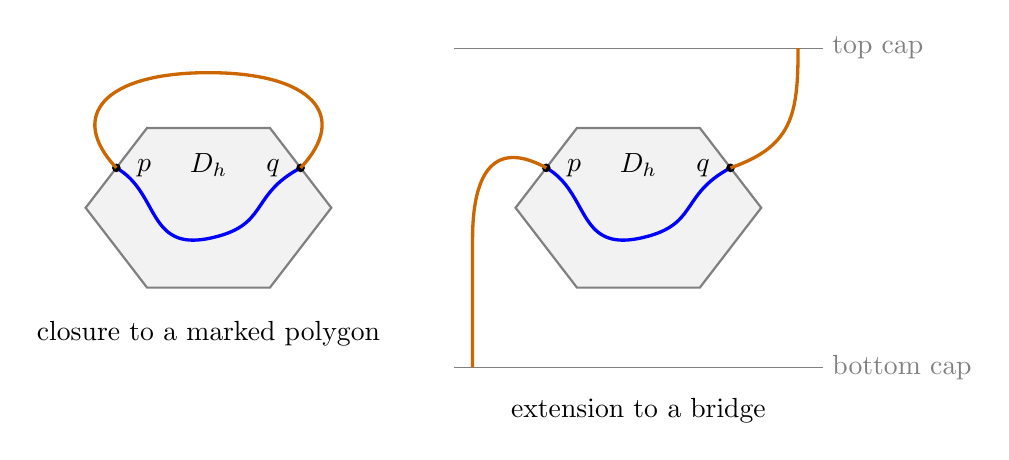
\begin{tikzpicture}[scale=.78,>=stealth]
\foreach \x in {0,7} {
  \begin{scope}[xshift=\x cm]
    \fill[gray!10] (-2,0)--(-1,-1.3)--(1,-1.3)--(2,0)--(1,1.3)--(-1,1.3)--cycle;
    \draw[gray,thick] (-2,0)--(-1,-1.3)--(1,-1.3)--(2,0)--(1,1.3)--(-1,1.3)--cycle;
    \draw[very thick,blue] (-1.5,.65) .. controls (-.8,.25) and (-1,-.7) .. (0,-.5)
      .. controls (1,-.3) and (.65,.2) .. (1.5,.65);
    \fill (-1.5,.65) circle(2pt) node[right=4pt] {$p$};
    \fill (1.5,.65) circle(2pt) node[left=4pt] {$q$};
    \node at (0,.7) {$D_h$};
  \end{scope}
}
\draw[very thick,orange!80!black] (-1.5,.65) .. controls (-2.3,1.5) and (-1.7,2.2) .. (0,2.2)
 .. controls (1.7,2.2) and (2.3,1.5) .. (1.5,.65);
\node at (0,-2.05) {closure to a marked polygon};
\begin{scope}[xshift=7cm]
 \draw[gray] (-3,2.6)--(3,2.6) node[right] {top cap};
 \draw[gray] (-3,-2.6)--(3,-2.6) node[right] {bottom cap};
 \draw[very thick,orange!80!black] (-1.5,.65) .. controls (-2.5,1.2) and (-2.7,.3) .. (-2.7,-.5)--(-2.7,-2.6);
 \draw[very thick,orange!80!black] (1.5,.65) .. controls (2.5,1) and (2.6,1.5) .. (2.6,2.6);
 \node at (0,-3.3) {extension to a bridge};
\end{scope}
\end{tikzpicture}
\caption{The two exterior sewing operations. The blue path is the chord being tested; the orange portions stay outside the convex domain. The proof realizes these schematic curves through pure-direction corridors and varies their intermediate cuts. The two boundary crossings recover the original chord for a fixed cut choice.}
\label{fig:sewing}
\end{figure}


\paragraph{Exterior connectors.}
Here are the geometric constructions and their mass bounds. For 1 close by a connector strictly in the exterior with diameter at most \(C l\), fixed endpoints \(p,q\), mass available \(\ge c l^{-5/4}\). For 2 append from \(p,q\) separate exterior paths to the two caps without touching either cap earlier, also within distance \(C R\) of the origin; together their available mass is at least \(cR^{-1/2}\exp[-C(1+\log^+(R/l))]\). In both cases for large \(l\) arrange that both exterior branches advance from their initial endpoints locally in disjoint patches of small size compared with \(l\) until reaching distance \(\rho l\) from \(D_h\), and all exterior portions between/beyond these visits stay at distance at least \(\rho l\) (sufficiently small fixed \(\rho>0\)). Even enlarged a little each patch sees only facets of a single consecutive-normal pair for outer and inner cuts used together below.

For 1, work in units \(l\), so the endpoints are separated. Take initial straight pieces along their respective outward pure normals, followed by two disjoint simple routes in the open exterior approaching a common terminal pure line from the same side in the pure perpendicular direction at two separated but close points. Around this terminal patch keep a free half-ball with radius much greater than the terminal separation (so the preceding confined arch lemma applies). The pieces other than this terminal arch can be made straight in pure directions with successive turns at most \(60^\circ\), each traveled by the point-to-line lemma with small tolerances. We give details justifying uniform finite choices in this assertion.

On scaling by \(l\) and translating, any sequence has a subsequence with distinct limit endpoints and exterior of a convex polygon, wedge or half-plane as local limit (and the indicated outward support normals among active ones). Initial rays give strictly positive distance by the corresponding supporting lines, then one can follow disjoint smooth arcs in the open exterior into an unobstructed ball for the parallel terminal lanes, approaching them on the same side. Indeed one can join the initial segments by a simple detour around the enlarged convex boundary in the connected exterior, and bend in a free middle ball to enter two parallel lanes separated by any sufficiently small distance. 

One can approximate the two arcs with end straight segments retained by polygonal arcs in pure directions: track tangent displacements on short intervals using the two adjacent pure directions spanning the tangent, inserting a short common-direction step at sector transitions, and adjusting the last intersections with the common line. Mesh sufficiently small gives separation for portions distant along the arcs, and on short portions tangent continuity gives positive projection in a common direction and hence simplicity (smooth arcs can be taken piecewise with finitely many sector transitions). Now use fixed sufficiently small apertures on the finitely many legs. End placement errors are also small by choosing tolerances small enough on all stages. Nonincident portions and successive crossing neighborhoods are separated. Along a path, adjacent pieces are disjoint by staying in the required half-planes at the transverse crossing between them; the initial piece stays in its supporting half-plane throughout. 

All choices still work along the subsequence, including the localized initial deep excursions. This gives uniformity of lengths, number of steps and apertures at this scale. For bounded \(l\), a local join at bounded cost outside suffices (exterior triangles at the two edges are connected by adjacencies around the convex flat patch or corner); no deep constraint needed.

For 2 if \(l\) is at least a fixed small multiple of \(R\), the same construction in units \(R\) suffices without terminal arch, following two disjoint paths to the two caps, terminating separately on each. Such paths exist with clearance in the intervening slab by routing in a wide annulus around the convex obstacle (in cyclic order to the outgoing lanes) before going straight to the caps. 

For smaller \(l\) the points lie on the same or adjacent facets. Start along divergent pure directions: on the same facet of normal \(m\) rotate \(m\) by \(60^\circ\) in opposite directions, heading away from one another; on adjacent facets use their two outward normals. Distances along the chosen straight rays from different ends at parameters \(x,y\ge0\) are separated by at least \(c(l+x+y)\) by projection onto the common separation tangent (bisecting the tangents for adjacent facets). Supporting normal height increases at rate at least \(1/2\). Travel to a small fixed distance of order \(R\) along each, first with a point-to-line crossing at scale \(l\), then confined pure bridges along the ray to successive heights growing by factor about 2. Tolerances a sufficiently small constant times the scales work simultaneously (error accumulation bounded geometrically); these paths are disjoint, exterior, and satisfy the initial depth condition. Continue from the macroscopically separated locations by finitely many legs at scales comparable with \(R\), as above. Uniformity here follows by the same compactness on scale \(R\) even if the rays had coincident limiting starts, since their terminal segments are already outgoing and separated in the open exterior and can be continued disjointly without meeting either ray again (route outside around the polygon and the two initial segments). The total number of legs is at most \(C(1+\log^+(R/l))\).

\paragraph{Averaging intermediate levels.}
Fix one of these corridor constructions and keep \(D_h,p,q\) fixed. In both cases, vary each intermediate transverse level uniformly over the admissible levels in its own small independent window of order the local scale, the terminal pure line for case 1 shared at both ends. Let \(\nu\) be critical weight on all exterior objects with the stated confinement and depth: a path from the labelled endpoint \(p\) to \(q\) in case 1, or an ordered pair of disjoint paths from \(p,q\) to their assigned caps in case 2. Weight counts all centers in these exterior paths. For a cut list \(\mathbf u\), let \(\mathbf1_{\mathbf u}(\eta)\) indicate that the exterior object \(\eta\) follows the prescribed corridors at those levels, and put
\[
 Y(\eta)=\mathbb E_{\mathbf u}\mathbf1_{\mathbf u}(\eta),
 \qquad P=\prod_{j=1}^k s_j^{-1/4}.
\]
Here \(s_j\) are the fixed reference scales of the \(k\) legs before any completing arch; their transverse cut separations vary within comparable windows. The indicator counts an exterior object once, since its transversal crossings recover all pieces for a fixed cut list. Concatenating the confined crossings gives
\[
 \int Y\,d\nu\ge
 \begin{cases}
 c^k l^{-5/4}P,&\text{in case 1},\\
 c^k P,&\text{in case 2},
 \end{cases}
\]
after reducing the constant \(c>0\) if necessary.

For two lists, split each branch at both choices of each varied crossing, encountered in height order in its own crossing neighborhood, yielding a difference bridge there. Indeed nonincident pieces stay out of this neighborhood, and between successive crossing stages from one end the two incident half-plane constraints put all crossings of that stage in order, with an intervening portion traveling to the next stage between its respective lines (a distance comparable to its scale). More explicitly both possible renewals in one neighborhood occur before entering the next neighborhood along the path, since the later pieces in each list avoid the former and earlier pieces avoid the latter; the crossing point for each choice is unique there and the branch locally before/after satisfies its backward/forward half-plane condition. Thus the intervening costs with incoming point prescribed are \(O(s_j^{-1/4})\) again by the upper point-to-line estimate. 

In case 1 the completing arch at the later shared level costs \(O(l^{-5/4})\) for any attained endpoints, and the shared difference gives two bridge costs of order \((1+|\mathrm{gap}|)^{-1/4}\) (the arch and the last incident pieces stay after/before the shared line, other pieces avoid this terminal patch including all confined arches). Averaging the joint costs supplies an extra \(s_j^{-1/4}\) for each varied renewal per branch at scale \(s_j\). The shared difference has power \(1/2\), so this average is still integrable. In case 2 only the two final cap levels are fixed; their endpoints remain free, and both final legs have scale comparable to \(R\). Consequently
\[
 \int Y^2\,d\nu\le
 \begin{cases}
 C^k l^{-5/4}P^2,&\text{in case 1},\\
 C^k R^{1/2}P^2,&\text{in case 2}.
 \end{cases}
\]
The factor \(R^{1/2}\) in the second line removes from the second copy of \(P\) the two factors corresponding to the fixed cap levels.

Cauchy--Schwarz now gives
\[
 \nu\{Y>0\}\ge\frac{(\int Y\,d\nu)^2}{\int Y^2\,d\nu}
 \ge
 \begin{cases}
 c_1^k l^{-5/4},&\text{in case 1},\\
 c_1^k R^{-1/2},&\text{in case 2},
 \end{cases}
\]
for a fixed \(0<c_1<1\). The number of legs is bounded in case 1. In case 2 it is at most \(C(1+\log^+(R/l))\), so \(c_1^k\ge c\min(1,(l/R)^{C_0})\) for a fixed \(C_0>0\). These are the asserted connector masses. The next average varies \(D_h\) itself, using these completed exterior objects.

\paragraph{A common target measure.}
Trim the exterior choices by fractional indicators down to precisely a common lower mass \(F\asymp l^{-5/4}\) or \(F\asymp R^{-1/2}\min(1,(l/R)^{C_0})\), respectively, pointwise for \(p,q,h,D_h\). The augmented object is a polygon injecting into the cylinder in 1 (both \(D_h\) and the augmentation near zero within a small fraction of the period length), or a full bridge in 2. For a fixed cut choice one recovers the decomposition up to bounded multiplicity since there are exactly two crossings of its boundary.

Here is the common measure used for the second moment. Let \(\Omega\) contain all six phase--slope pairs, with their product probability law, and let \(\mu\) be critical weight on target polygons through the prescribed links, or on target bridges satisfying the common deterministic event in 2. Its total mass is at most \(\mathcal K\) or \(B^*\), respectively. In a level window \(I\) of size comparable to \(\epsilon l\), define \(b_h(\Gamma,\Omega)\) to be the sum over recovered ordered decompositions of \(\Gamma\) at \(\partial D_h\) of the chord-event indicator times the exterior trimming factor. The recovery bound gives \(0\le b_h\le C\). Put
\[
 X(\Gamma,\Omega)=\mathop{\mathrm{average}}_{h\in I}
 b_h(\Gamma,\Omega).
\]
The overbar below includes both this level average and support randomness. Weight multiplication and recovery give
\begin{equation}\label{eq:sewing-first-moment}
 \int X\,d(\mu\otimes\mathbb P_\Omega)\asymp F\overline E.
\end{equation}
Both factors in \(X^2\) are tested on the same target \(\Gamma\) and the same \(\Omega\).

Choose the two levels independently and uniformly in \(I\). By symmetry it suffices to integrate over \(r<s\), with the original product measure restricted to this half-square, plus any diagonal atoms. This restriction is not renormalized: conditional on \(r\), the remaining \(s\)-measure has density, or rounded atom mass, at most \(C/l\). For \(\epsilon>0\) sufficiently small, a simultaneous event splits into the chord event for \(D_r\), two exterior bridges crossing the band to \(\partial D_s\), and then the augmentation from there; keep only the latter trimming factor. Boundary crossings are unique on the separate branches, localized by the depth condition because the boundary moves by at most \(C\epsilon l+O(1)\). For bounded \(s-r\), or bounded \(l\), the indicator at \(r\) alone suffices. We will bound the averaged cost \(\Xi\) of the two band bridges uniformly conditional on the inner level and phases. This gives
\begin{equation}\label{eq:sewing-second-moment}
 \int X^2\,d(\mu\otimes\mathbb P_\Omega)
 \le CF\overline E\,\Xi.
\end{equation}

\paragraph{The two band bridges.}
Put \(g=s-r\). We bound the bridges for large \(g\) as follows. Fix for each bridge the possible target normal in the local facet pair. Drop all other outer cuts, keeping the entire inner elbow in a local patch with two lateral pure trims transversal to both tangent directions containing the bridge portions; the domain is a polygonal strip between this outward cut line and the flat or elbow piece of \(D_r\). The inner obstacle here keeps just the two corresponding consecutive constraints (or just one for a common flat region), extended throughout the strip patch; this agrees locally on the required bridge portions. The target outward cut line is thus disjoint from it by the positive gap. Trims may for instance bound projection on the common tangent bisector for a consecutive pair (a pure normal direction), wide enough to enclose the localized portions and leave clearance at the source, and can be fixed independently of the dropped outer facets. 

There is a positive contour (after a possible rotation) from the inner source. Indeed closing a chord along the boundary gives \(W\) equal to lifted outward-normal change minus \(\pi\) going round the counterclockwise perimeter from source to exit. There is only one possible reflex corner on the inner elbow, with outward normal decreasing by \(\pi/3\), and its two outward normals and the outward normals on trim sides and target line are in cyclic order except for this one corner (the trims use a pure direction strictly between opposing boundary sectors). Thus from a given inner source at most one sign of excess beyond \([-\pi,\pi]\) occurs, and by at most \(\pi/3\); rotating gives real coefficients bounded below positively since \(\beta=3/8\). Convexity is not needed for the contour identity on this simply connected domain. 

Cut down by a centered triangle at scale a small multiple of \(\min(g,t_i)\), where the inner source is on a flat side. By contour subtraction and the escape upper estimate its bridge cost is \(O((1+\min(g,t_i))^{-1/4})\). This also holds by the full positive contour when the minimum is bounded. 

For the corner gain, put \(t=\min_i t_i\). Both tests in \(X^2\) use the same dyadic endpoint bins: the two inner bin sizes are at least \(t\), and one outer bin has size of order \(t\). Sum over the finitely many choices of that outer endpoint and of the facet it reaches. For each choice, condition on the six phases at \(r\), making the inner chord event measurable, and on the support position of the selected target facet at \(s\). Figure~\ref{fig:sewing-band} shows the adjacent outer facet whose support has not been revealed.
\begin{figure}[htbp]
\centering
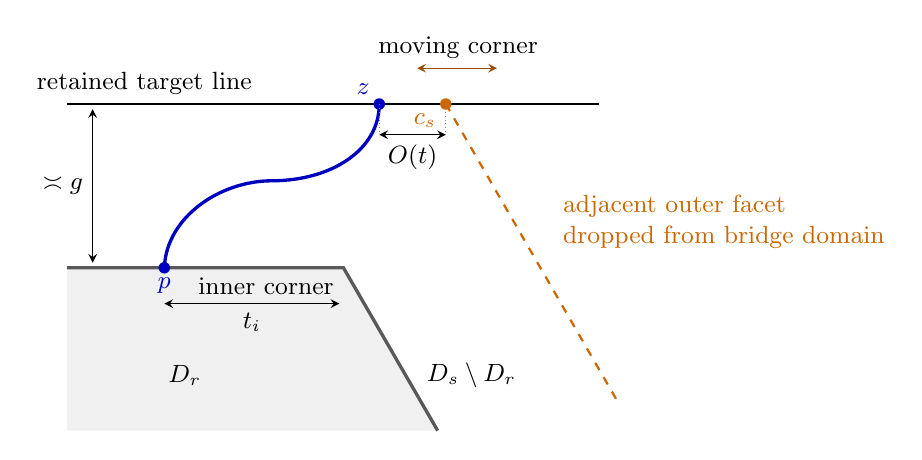
\begin{tikzpicture}[scale=1.3,>=stealth,font=\small]
 \fill[gray!12] (-2.7,0)--(0,0)--(.92,-1.59)--(-2.7,-1.59)--cycle;
 \draw[gray!70!black,very thick] (-2.7,0)--(0,0)--(.92,-1.59);
 \node at (-1.55,-1.05) {$D_r$};
 \node at (1.25,-1.05) {$D_s\setminus D_r$};
 \node[below left] at (0,0) {inner corner};
 \draw[thick] (-2.7,1.6)--(2.5,1.6);
 \node[above left] at (-.8,1.6) {retained target line};
 \draw[orange!80!black,thick,dashed] (1,1.6)--(2.7,-1.344);
 \draw[orange!60!black,<->] (.72,1.95)--(1.5,1.95);
 \node[above] at (1.12,1.95) {moving corner};
 \node[orange!80!black,align=left,anchor=west] at (2.05,.45)
   {adjacent outer facet\\dropped from bridge domain};
 \fill[orange!80!black] (1,1.6) circle(1.6pt) node[below left] {$c_s$};
 \draw[blue!75!black,very thick] (-1.75,0)
   .. controls (-1.73,.5) and (-1.2,.85) .. (-.7,.85)
   .. controls (-.12,.85) and (.35,1.15) .. (.35,1.6);
 \fill[blue!75!black] (-1.75,0) circle(1.6pt) node[below] {$p$};
 \fill[blue!75!black] (.35,1.6) circle(1.6pt) node[above left] {$z$};
 \draw[<->] (.35,1.3)--(1,1.3) node[midway,below] {$O(t)$};
 \draw[gray,densely dotted] (.35,1.6)--(.35,1.3);
 \draw[gray,densely dotted] (1,1.6)--(1,1.3);
 \draw[<->] (-1.75,-.35)--(-.04,-.35) node[midway,below] {$t_i$};
 \draw[<->] (-2.45,.05)--(-2.45,1.55) node[midway,left] {$\asymp g$};
\end{tikzpicture}
\caption{The selected band bridge from an inner port $p$ to an outer port $z$, with $g=s-r$. The inner elbow is retained when bounding the bridge, while the dashed adjacent outer facet is dropped. After fixing the target support, the adjacent support is still independent and has conditional density, or row-atom bound, $O(1/g)$. Its intersection $c_s$ with the target therefore falls within $O(t)$ of a fixed $z$ with probability at most $C\min(1,t/(1+g))$, including row rounding. The diagram is schematic; the second band bridge is bounded uniformly without revealing this support.}
\label{fig:sewing-band}
\end{figure}


For any attained outer endpoints and support choices, integrate the outer completion to its constant trimmed mass \(F\). Bound the other band bridge uniformly after dropping its extra avoidance constraints. This bound does not require revealing the adjacent outer support, even if the other bridge ends on that facet.

The adjacent outer facet defining the selected endpoint's corner is therefore still unconditioned. Its position is independent of the selected target support, conditional on the inner phases, and has density \(O(1/g)\). This remains true because \(V_i+A_i r/R\) modulo one is uniform and independent of \(A_i\). Since that adjacent facet was dropped from the selected bridge domain, each possible end has probability at most \(C\min(1,t/(1+g))\) of being within \(O(t)\) of its corner, also after lattice rounding. We average this corner event instead of conditioning on it. Both inner endpoint bin sizes are at least \(t\), so the product of the two bridge bounds is uniform in the support parameter still being averaged. The resulting joint cost is therefore
\[
 C(1+\min(g,t))^{-1/2}\min\{1,t/(1+g)\}
 \le C(1+g)^{-1/2}.
\]

The conditional gap estimate gives \(\Xi\le Cl^{-1/2}\) on each window. Applying Cauchy--Schwarz to \eqref{eq:sewing-first-moment}--\eqref{eq:sewing-second-moment} yields
\[
 \overline E\le C\mathcal K\,\Xi/F,
 \qquad B^*\ge cF\overline E/\Xi,
\]
respectively. Substitution of \(F\) and \(\Xi\) proves both sewing assertions. Averaging these inequalities recombines the windows.
\end{proof}

\subsection{Corner gains and the marked-pair sum}\label{sec:corner-sum}

The previous estimate is sufficient for one endpoint bin. To sum all bins with a bounded constant, we retain the gain when an endpoint lies close to a corner. Write $t=\min(t_1,t_2)$, with $1\le t\le l$. The two estimates before averaging the cut gap $g$ give the combined cost
\[
 C(1+\min(g,t))^{-1/2}\min\{1,t/(1+g)\}.
\]
For each fixed inner level $r$, the unnormalized gap law on the half-square $r<s$ has density at most $C/l$ over an interval of length $O(l)$, with the analogous bound for its rounded discrete law. This uniformity allows the estimate to be integrated against the possibly nonconstant mass $E_r$. Splitting at $g=t$ shows that its average is at most
\[
 \frac C l\left(\int_0^t(1+g)^{-1/2}\,dg
 +t(1+t)^{-1/2}\int_t^{Cl}\frac{dg}{1+g}\right)
 \le C_\eta l^{-1/2}(t/l)^\eta
\]
for any fixed $0<\eta<1/2$. The bounded-gap atoms satisfy the same estimate after increasing $C_\eta$.

Keeping this gain in the first sewing argument gives
\begin{equation}\label{eq:sewing-corner-gain}
 \overline E\le C_\eta l^{3/4}(t/l)^\eta\mathcal K.
\end{equation}
Indeed the first moment in the target polygon measure is at least $cF\overline E$, while the second is at most
$CF\overline E\,l^{-1/2}(t/l)^\eta$; use $F\asymp l^{-5/4}$. For each smaller corner bin $t$, the larger one has only $O(1+\log(l/t))$ possible dyadic values. Thus their total contribution is bounded by
\[
 C_\eta\sum_{j\ge0}(1+j)2^{-j\eta}<\infty.
\]
The same summation shows that bins with $t/l\le\delta$ have total coefficient tending to zero as $\delta\downarrow0$.

Let $\ell_h$ denote the length of a chord in $D_h$, and retain chords of diameter at least $R/3$. Their mass is at most $CR^{3/4}$. Their first-length mass is at least $cR^{25/12}$: every path through a sufficiently central link is macroscopic, and Proposition~\ref{prop:occupancy} with Theorem~\ref{thm:nesting} supplies mass at least $cR^{1/12}$ at each of $cR^2$ such links. The upper first-length mass over all chords is $CR^{25/12}$ by the same identity.

To estimate the second moment, first omit the initial and terminal visited centers. The ordered pairs involving these at most two centers number $O(\ell_h)$, so their integrated contribution is absorbed by the first-length bound. At each remaining center, record the directions of the two tiling edges crossed by its incident path links. Divide these centers into finitely many classes according to triangle type, lattice translation modulo two, and that pair of tiling-edge directions. The square of the total number of remaining centers is bounded by a fixed multiple of the sum of the squares of the class counts. Within a class, pairs with axial or zero displacement contribute at most $CR\ell_h$ for each chord: a bounded domain of diameter $CR$ has only $CR$ positions on the finitely many axial lines through a given center. Their integrated contribution is therefore at most $CR^{37/12}$.

For a remaining ordered pair, choose the two lattice axes spanning the strict sector containing its displacement. At least one of the two recorded tiling-edge directions is one of those axes. Since the two centers have the same triangle type, the corresponding crossed edges are translates and supply identical axial marks used by internal links of the chord. Their displacement has even coordinates in the chosen lattice basis, by the translation class modulo two. Hence $d=P_1+P_2$ is even, as required in Theorem~\ref{thm:two-marks}. Choose an integer period multiple $kP$ with length comparable to a sufficiently large constant times $R$, so the sewn polygon projects injectively. Then $N\asymp R$ and
\[
 \mathcal K\le C R^{-4/3}(R/d)^{15/8}.
\]
There are $O(R^2)$ choices of the first center and $O(d)$ displacements with $P_1+P_2=d$. Consequently
\begin{equation}\label{eq:marked-pair-sum}
 \sum_{\text{eligible pairs}}\mathcal K
 \le CR^2R^{-4/3}R^{15/8}\sum_{1\le d\le CR}d^{1-15/8}
 \le CR^{8/3}.
\end{equation}
Apply \eqref{eq:sewing-corner-gain} to each pair event. The corner bins sum with bounded total coefficient, and the separation factors $l^{3/4}$ sum geometrically up to $CR$. We obtain
\begin{equation}\label{eq:chord-second-moment}
 \overline{\sum_{\gamma\text{ macroscopic in }D_h}
       \ell(\gamma)^2w(\gamma)}\le CR^{41/12}.
\end{equation}
The contribution from bins $l\le\delta R$ has upper bound
$C\delta^{3/4}R^{41/12}+CR^{37/12}$. On the remaining separations, bins with $t\le\delta'R$ likewise have arbitrarily small relative coefficient when $\delta'$ is sufficiently small. These are estimates for actual endpoint restrictions on the chords, not an assumption that endpoints avoid corners.

\subsection{A positive fraction of long bridges}

We now prove \eqref{eq:bridge-long-fraction}. Write $M_1$ for the averaged first-length mass of the macroscopic chords. We have $M_1\ge c_1R^{25/12}$. By Cauchy--Schwarz, a class with second moment at most $\varepsilon R^{41/12}$ contributes at most
\[
 (CR^{3/4}\cdot\varepsilon R^{41/12})^{1/2}
 =C\sqrt\varepsilon\,R^{25/12}
\]
to $M_1$. Choose $\delta>0$ and then $\delta'>0$ so that removal of close endpoints and small corner bins loses less than one quarter of $M_1$. Chords shorter than $aR^{4/3}$ contribute at most $CaR^{25/12}$, which is less than another quarter if $a>0$ is fixed sufficiently small.

The retained chords therefore have averaged first-length mass at least $c_2R^{25/12}$. Their endpoint separation and corner distances are all bounded below by fixed multiples of $R$, so they occupy only a bounded number of bins. In at least one bin the first-length mass has the same lower order. Applying Cauchy--Schwarz to that bin and \eqref{eq:chord-second-moment} gives its averaged ordinary mass at least
\[
 c\frac{R^{50/12}}{R^{41/12}}=cR^{3/4}.
\]
The second sewing estimate extends these chords to bridges between any prescribed pair of horizontal caps whose distances above and below the origin lie in $[AR,2AR]$, for a fixed sufficiently large $A$. Since $l\asymp R$, that estimate gives total bridge mass at least $cR^{3/4}$ when the bottom start is free over the permitted interval of $O(R)$ ports. Every output bridge contains the retained chord, and hence has length at least $aR^{4/3}$.

Translation invariance makes the unrestricted mass from each bottom port equal. Removing the confinement and dividing by the number of permitted starting ports yields
\[
 B_h\{\ell\ge aR^{4/3}\}\ge cR^{-1/4}
\]
for every admissible cap separation $h d_0\in[2AR,4AR]$. For an arbitrary sufficiently large integer $h$, choose $R$ proportional to $h$ so the selected caps lie in these ranges; admissible rounding changes only fixed constants. This proves \eqref{eq:bridge-long-fraction} at every sufficiently large height.

\subsection{The strip first moment and completion of the proof}

It remains to prove the first-length upper bound. In the infinite strip, summing occurrences of internal links over bridges from one fixed bottom port is the same as summing the occurrence mass with free bottom port over link representatives modulo translations along the strip. There are $O(h)$ such representatives. Proposition~\ref{prop:occupancy}, first in finite convex truncations and then by monotone exhaustion, bounds the occurrence mass at each link by the positive enclosing-polygon partitions at its adjacent lattice points.

These partitions are at most $Ch^{1/12}$ even though the strip is infinite. To see this, take a pure lattice period vector tilted relative to the strip's horizontal tangent, of sufficiently large even length comparable to $h$, with transverse projection greater than $2h d_0$. The strip and its translate by half this period embed disjointly in the resulting cylinder. The disk enclosed by each polygon stays inside its convex strip, so it cannot contain the mark in the translated strip. Thus two independent systems enclosing corresponding points inject into a system separating the antipodal marks. The bounded-factor cylinder estimate in Section~\ref{sec:uniform-nesting} is at most $Ch^{1/6}$, so the square of the strip partition is at most that quantity.

Summing over the $O(h)$ link representatives gives
\[
 \sum_{\gamma\in\mathcal B_h}(\ell(\gamma)-1)w(\gamma)
 \le Ch^{13/12}.
\]
The missing one center per bridge adds only $B_h\le Ch^{-1/4}$. This proves \eqref{eq:bridge-first-moment}. The strip mass \eqref{eq:bridge-mass} was proved in Sections~\ref{c6:strip-transfer}--\ref{c6:strip-asymptotics}, and Proposition~\ref{prop:crossings} gives \eqref{eq:bridge-diameter}. Theorem~\ref{thm:finite-bridges} is complete.

\begin{thebibliography}{99}
\raggedright
\bibitem{BeatonEtAl2014}
N.~R.~Beaton, M.~Bousquet-M\'elou, J.~de Gier, H.~Duminil-Copin and A.~J.~Guttmann.
The critical fugacity for surface adsorption of self-avoiding walks on the honeycomb lattice is $1+\sqrt2$.
\emph{Communications in Mathematical Physics} \textbf{326} (2014), 727--754.
\href{https://doi.org/10.1007/s00220-014-1896-1}{doi:10.1007/s00220-014-1896-1}.
\href{https://arxiv.org/abs/1109.0358}{arXiv:1109.0358}.

\bibitem{Bogso2014}
A.~M.~Bogso.
An application of multivariate total positivity to peacocks.
\emph{ESAIM: Probability and Statistics} \textbf{18} (2014), 514--540.
\href{https://doi.org/10.1051/ps/2013049}{doi:10.1051/ps/2013049}.

\bibitem{DiFrancescoZinnJustin2005}
P.~Di Francesco and P.~Zinn-Justin.
Around the Razumov--Stroganov conjecture: proof of a multi-parameter sum rule.
\emph{Electronic Journal of Combinatorics} \textbf{12} (2005), Research Paper~6.
\href{https://doi.org/10.37236/1903}{doi:10.37236/1903}.
\href{https://arxiv.org/abs/math-ph/0410061}{arXiv:math-ph/0410061}.

\bibitem{DuminilCopinSmirnov2012}
H.~Duminil-Copin and S.~Smirnov.
The connective constant of the honeycomb lattice equals $\sqrt{2+\sqrt2}$.
\emph{Annals of Mathematics} \textbf{175} (2012), 1653--1665.
\href{https://doi.org/10.4007/annals.2012.175.3.14}{doi:10.4007/annals.2012.175.3.14}.

\bibitem{Frenkel1985}
I.~B.~Frenkel.
Representations of Kac--Moody algebras and dual resonance models.
In \emph{Applications of Group Theory in Physics and Mathematical Physics}
(Chicago, 1982), Lectures in Applied Mathematics \textbf{21},
American Mathematical Society, Providence, RI, 1985, 325--353.
\href{https://cpb-us-w2.wpmucdn.com/campuspress.yale.edu/dist/2/3739/files/2021/06/frenkel_representations_kac_moody.pdf}{Author's copy}.

\bibitem{FrenkelKac1980}
I.~B.~Frenkel and V.~G.~Kac.
Basic representations of affine Lie algebras and dual resonance models.
\emph{Inventiones Mathematicae} \textbf{62} (1980), 23--66.
\href{https://doi.org/10.1007/BF01391662}{doi:10.1007/BF01391662}.

\bibitem{GarbaliNienhuis2017Ground}
A.~Garbali and B.~Nienhuis.
The dilute Temperley--Lieb $O(n=1)$ loop model on a semi infinite strip:
the ground state.
\emph{Journal of Statistical Mechanics: Theory and Experiment} (2017), 043108.
\href{https://doi.org/10.1088/1742-5468/aa6a30}{doi:10.1088/1742-5468/aa6a30}.
\href{https://arxiv.org/abs/1411.7020}{arXiv:1411.7020}.

\bibitem{GarbaliNienhuis2017Sum}
A.~Garbali and B.~Nienhuis.
The dilute Temperley--Lieb $O(n=1)$ loop model on a semi infinite strip:
the sum rule.
\emph{Journal of Statistical Mechanics: Theory and Experiment} (2017), 053102.
\href{https://doi.org/10.1088/1742-5468/aa6bc3}{doi:10.1088/1742-5468/aa6bc3}.
\href{https://arxiv.org/abs/1411.7160}{arXiv:1411.7160}.

\bibitem{GlazmanManolescu2017}
A.~Glazman and I.~Manolescu.
Self-avoiding walk on $\mathbb Z^2$ with Yang--Baxter weights:
universality of critical fugacity and 2-point function.
\emph{Annales de l'Institut Henri Poincar\'e, Probabilit\'es et Statistiques}
\textbf{56} (2020), 2281--2300.
\href{https://doi.org/10.1214/19-AIHP1024}{doi:10.1214/19-AIHP1024}.

\bibitem{GrimmPearce1993}
U.~Grimm and P.~A.~Pearce.
Multi-colour braid--monoid algebras.
\emph{Journal of Physics A: Mathematical and General} \textbf{26} (1993), 7435--7460.
\href{https://doi.org/10.1088/0305-4470/26/24/018}{doi:10.1088/0305-4470/26/24/018}.
\href{https://arxiv.org/abs/hep-th/9303161}{arXiv:hep-th/9303161}.

\bibitem{HilgertRilke2008}
J.~Hilgert and F.~Rilke.
Meromorphic continuation of dynamical zeta functions via transfer operators.
\emph{Journal of Functional Analysis} \textbf{254} (2008), 476--505.
\href{https://doi.org/10.1016/j.jfa.2007.10.003}{doi:10.1016/j.jfa.2007.10.003}.
\href{https://arxiv.org/abs/math/0701097}{arXiv:math/0701097}.

\bibitem{IshikawaOkadaTagawaZeng2006}
M.~Ishikawa, S.~Okada, H.~Tagawa and J.~Zeng.
Generalizations of Cauchy's determinant and Schur's Pfaffian.
\emph{Advances in Applied Mathematics} \textbf{36} (2006), 251--287.
\href{https://doi.org/10.1016/j.aam.2005.07.001}{doi:10.1016/j.aam.2005.07.001}.

\bibitem{KrachunPanagiotis2026}
D.~Krachun and C.~Panagiotis.
Quantitative sub-ballisticity of self-avoiding walk on the hexagonal lattice.
\emph{Annals of Probability} \textbf{54} (2026), 1109--1125.
\href{https://doi.org/10.1214/24-AOP1730}{doi:10.1214/24-AOP1730}.
\href{https://arxiv.org/abs/2310.17299}{arXiv:2310.17299}.

\bibitem{Nienhuis1982}
B.~Nienhuis.
Exact critical point and critical exponents of $O(n)$ models in two dimensions.
\emph{Physical Review Letters} \textbf{49} (1982), 1062--1065.
\href{https://doi.org/10.1103/PhysRevLett.49.1062}{doi:10.1103/PhysRevLett.49.1062}.

\bibitem{Segal1981}
G.~Segal.
Unitary representations of some infinite dimensional groups.
\emph{Communications in Mathematical Physics} \textbf{80} (1981), 301--342.
\href{https://doi.org/10.1007/BF01208274}{doi:10.1007/BF01208274}.

\bibitem{TracyWidom1998}
C.~A.~Tracy and H.~Widom.
Correlation functions, cluster functions and spacing distributions for random matrices.
\emph{Journal of Statistical Physics} \textbf{92} (1998), 809--835.
\href{https://doi.org/10.1023/A:1023084324803}{doi:10.1023/A:1023084324803}.

\bibitem{ZhouBatchelor1997}
Y.~K.~Zhou and M.~T.~Batchelor.
Critical behaviour of the dilute $O(n)$, Izergin--Korepin and dilute
$A_L$ face models: Bulk properties.
\emph{Nuclear Physics B} \textbf{485} (1997), 646--664.
\href{https://doi.org/10.1016/S0550-3213(96)00654-2}{doi:10.1016/S0550-3213(96)00654-2}.
\href{https://arxiv.org/abs/cond-mat/9611156}{arXiv:cond-mat/9611156}.

\end{thebibliography}
\end{document}
